\documentclass[phd,12pt]{psuthesis}

% Declaration of all the packages used
\usepackage{amsmath}
\usepackage{amssymb}
\usepackage{amsthm}
\usepackage{exscale}
\usepackage[mathscr]{eucal}
\usepackage{bm}
\usepackage{eqlist} % Makes for a nice list of symbols.
\usepackage[final]{graphicx}
\usepackage{subcaption}
\usepackage[dvipsnames]{color}
\DeclareGraphicsExtensions{.pdf, .jpg, .png}
\usepackage{natbib}
\usepackage{har2nat}
\usepackage{verbatim}
\usepackage{url}
\usepackage{longtable}
\usepackage{mathpazo}
\usepackage{pstricks}
\usepackage{sgamevar}
\usepackage{slashbox}
\usepackage{multirow}
\usepackage{egameps}
\def\citeapos#1{\citeauthor{#1}'s \citeyear{#1}}
\newenvironment{my_enumerate}
{\begin{enumerate}
  \setlength{\itemsep}{1pt}
  \setlength{\parskip}{0pt}
  \setlength{\parsep}{0pt}}{\end{enumerate}}
\newenvironment{my_itemize}
{\begin{itemize}
  \setlength{\itemsep}{1pt}
  \setlength{\parskip}{0pt}
  \setlength{\parsep}{0pt}}{\end{itemize}}
\usepackage{algorithm}
\usepackage{algpseudocode}
\usepackage{tikz}
\let\clipbox\relax
\usepackage[export]{adjustbox}
\usetikzlibrary{shapes.geometric, arrows} %https://www.sharelatex.com/blog/2013/08/29/tikz-series-pt3.html
\usepackage{xcolor}
\usetikzlibrary{decorations.pathreplacing}
\usepackage{bm}

\usepackage[colorlinks=true,urlcolor=purple,citecolor=blue,linkcolor=blue]{hyperref}
\renewcommand{\theHchapter}{\thepart.\thechapter}

%\input{SupplementaryMaterial/UserDefinedCommands}

\renewcommand{\floatpagefraction}{0.85}
\renewcommand{\topfraction}      {0.85}
\renewcommand{\bottomfraction}   {0.85}
\renewcommand{\textfraction}     {0.15}

\title{Uncertainty Propagation Methods for High-Dimensional Complex Systems}
\author{Arpan Mukherjee}
\degreedate{February 2018}
\copyrightyear{2018}

\documenttype{Dissertation}
%The department where you will be submitting the document%
\dept{Department of Mechanical and Aerospace Engineering}
% This will generally be The Graduate School, though you can
% put anything in here to suit your needs. This has also been removes from the cover page via the psuthesis.cls document because UB guidelines do not allow for it.
\submittedto{The Graduate School}

\numberofreaders{4}

\advisor[Thesis Advisor, Chair of Committee]
        {Rahul Rai}
        {Associate Professor of Mechanical and Aerospace Engineering}

\readerone[Committee Member]
          {Puneet Singla}
          {Associate Professor of Mechanical and Aerospace Engineering}     			

\readertwo[Committee Member]
          {Tarunraj Singh}
          {Professor of Mechanical and Aerospace Engineering} 

\readerthree[Committee Member]
            {Abani Patra}
            {Professor of Mechanical and Aerospace Engineering} 

\readerfour[Outside Reader]
            {Anurag Purwar}
            {Research Associate Professor of Mechanical Engineering \newline Stony Brook University, The State University of New York}


\doublespacing
\includeonly{
Chapters/Introduction,
Chapters/UQ,
Chapters/WCS,
Chapters/SCS,
Chapters/Building,
Chapters/DEM,
Chapters/Conclusion,
}

\begin{document}
\frontmatter
\psutitlepage

%Generates Copyright Page
\copyrightpage{SupplementaryMaterial/Copyright}

\newpage
% Generates the committee page -- this is bound with your
% thesis. If this is an baccalaureate honors thesis, then
% comment out this line.
\psucommitteepage

% Generates the Epigraph/Dedication. The first argument should
% point to the file containing your Epigraph/Dedication and
% the second argument should be the title of this page.
\thesisdedication{SupplementaryMaterial/Dedication}{Dedication}

% Generates the Acknowledgments. The argument should point to
% the file containing your Acknowledgments.
\thesisacknowledgments{SupplementaryMaterial/Acknowledgments}

% Generates the Table of Contents
\thesistableofcontents

% Generates the List of Tables
\listoftables

% Generates the List of Figures
\listoffigures

\thesisabstract{SupplementaryMaterial/Abstract}

\thesismainmatter


\chapter{Introduction}

Physical processes are often modeled as complex nonlinear differential equations. A large number of state variables are usually involved in modeling the to have a better understanding of the system in question. Additionally, the presence of uncertainty in the state variables or parameters engaged in physics-based models is highly probable. Uncertainty Quantification (UQ) is used as a tool to enable rigorous prediction modeling. UQ by analytic methods of high-dimensional systems is computationally intractable due to the well-known phenomenon of \textit{curse of dimensionality}. For a large state space systems, conventional UQ methods become ineffective due to significant error in the approximation with propagation. A large number of sample points make simulation-based approaches very computationally intensive requiring high memory usage. Figure~\ref{uncp} illustrates the propagation of uncertainty in a large number of state variables via a given dynamical system. The resultant pdf is high-dimensional and difficult to estimate by analytical or even by established numerical techniques. 


\begin{figure}[H]
\centering
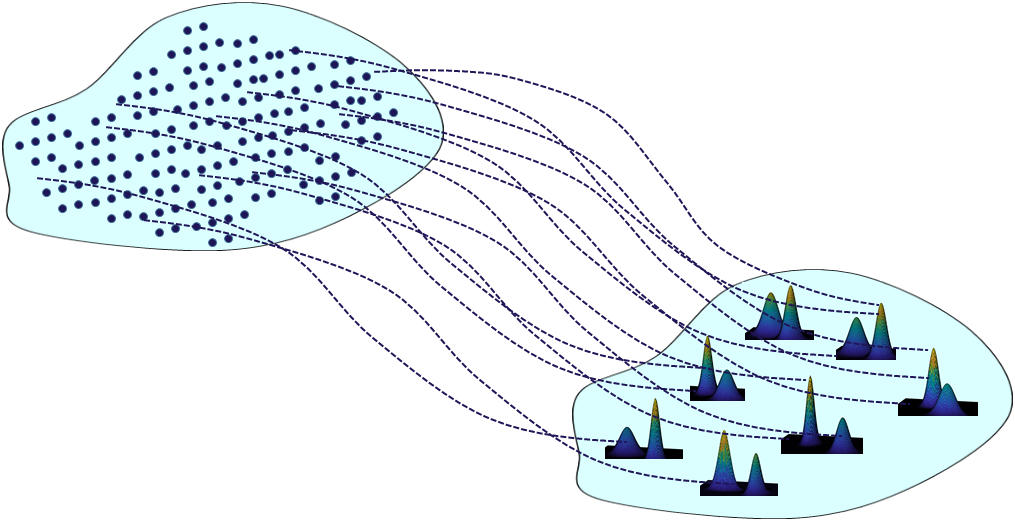
\includegraphics[width=\textwidth]{intr_figs/uncp}
\caption{Propagation of uncertainty via large dynamical system}
\label{uncp}
\end{figure}

Fortunately, many systems of importance as a general rule comprise of a very large number of interacting subsystems. Large systems comprising of interconnected subsystems have been studied in details~\cite{hale1997diffusive, afraimovich1997synchronization, fujisaka1983stability, martynyuk2012weakly}. Applications of such systems can be found in mechanical and electric systems~\cite{silver1967multiple, belykh1993chaotic, ji2012adaptive, georgiou2015multi}, biological networks~\cite{winfree1967biological, cohen1982nature, kopell1986symmetry, mirollo1990synchronization, ermentrout1998minimal} and laser arrays~\cite{winful1988stability, li1992preferential}. To make rigorous UQ of high dimension problem \textit{feasible}, it is prudent, if not imperative, to utilize the strategy of \textit{divide and conquer}. This dissertation utilizes the concept of system decomposition to decompose the overall system into multiple smaller subsystems to accelerate the UQ calculation for high-dimensional dynamical systems. The UQ analysis for the overall system is carried out by agglomerating results of UQ techniques on smaller subsystems. Consequently, it is of fundamental importance to understand why and under what conditions a high-dimensional state space system can be decomposed into a set of smaller subsystems. 

Physics-based models are described as a set of Ordinary or Partial Differential Equations (ODE/PDE). In most cases, the involved PDE is discretized using a numerical technique to a system of ODEs. The work outlined in this dissertation focuses on UQ of ODEs and then extend the framework to enable UQ of PDE based systems. 
Let us consider a complex dynamical system with state space specified by vector $\mathbf{x} = \{ x_1, x_2,..., x_n\}$ whose dynamics is governed by time-evolution equation $\dot{\mathbf{x}}_{t} = f(\textbf{x}_{t})$, where $t \in \mathbb{R}^+$ represents time. In a general setting, each state space variable is coupled with all other state space variables of the system. However, most often the inter-variable coupling (weak/strong) can be quantified and utilized to decompose the overall system into a set of smaller subsystems that can be solved in parallel (Figure~\ref{fig:UQframework}). In this context, following research challenges need to be answered.


\begin{figure}[H]
\centering
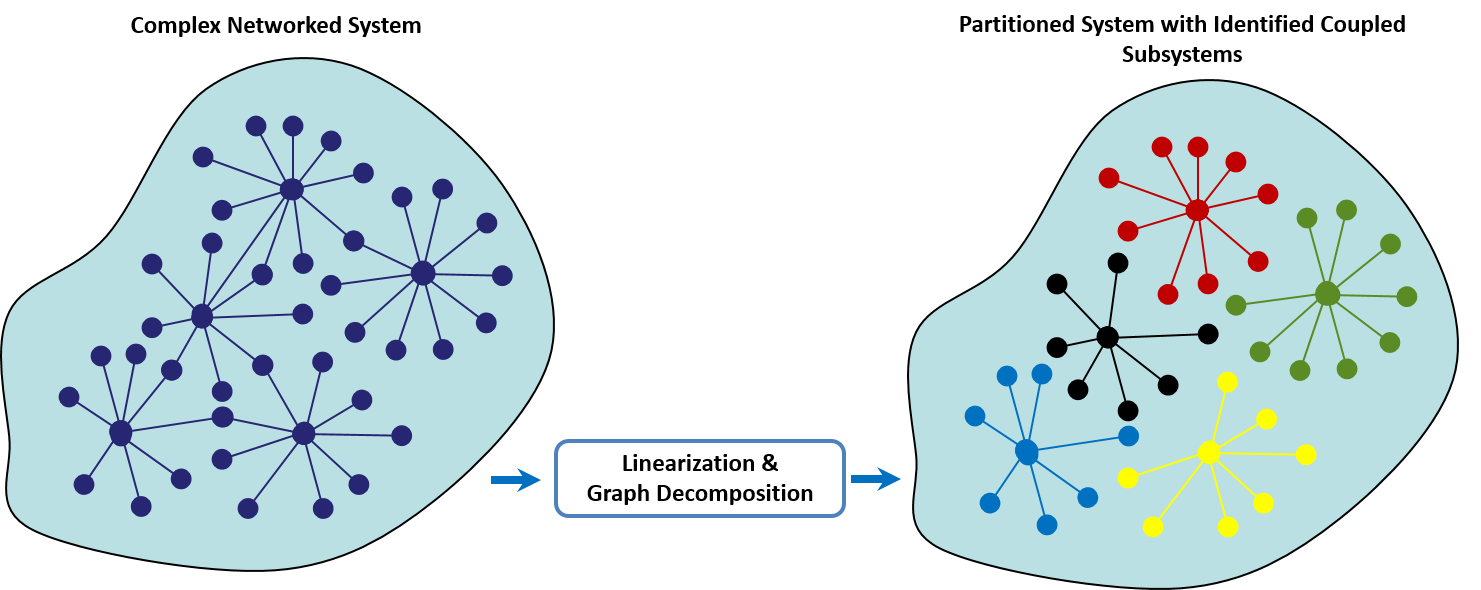
\includegraphics[width=\textwidth]{figures/FIG_1}
\caption{Modeling of the stochastic nonlinear system as an undirected graph}
\label{fig:UQframework}
\end{figure}

\section{Research Challenges}

The main research challenges in this dissertation can be outlined as:
\begin{itemize}
\item Given a dynamical system with defined equation and uncertain state variables/parameters, what is the best way to quantify the inter-state couplings? How can such quantification be used to partition the state space to a set of subsystems? 
\item Given the inter-state coupling what is the best way to decompose the state-space into subsets? How do the subsets behave individually and how is that behavior different from the aggregate of the subsystems and how can the behavior be quantified? 
\item What is the best way to integrate the state-space decomposition framework existing UQ methods?
%\item How can one approximately quantify the difference in the individual behavior of the subsystems? 
\item How can the decomposition method be extended to a continuous set of random variables or random field? In other words, can the technique apply to problems characterized by spatiotemporal flow equations or partial differential equations (PDE)? If yes, then how does the continuity of the random process be ensured by the decomposition technique?
\end{itemize}

The main contributions of this dissertation are in addressing the research challenges mentioned above.


\section{Contributions}

The concept of system decomposition is utilized to decompose the overall system into multiple smaller subsystems to accelerate the UQ calculation for high-dimensional dynamical systems. The UQ analysis for the overall system is carried out by agglomerating results of UQ techniques on smaller subsystems. The main contribution of this dissertation is two-fold which are described next.

\subsection{Contribution 1: Identification of Weakly Connected Subsystems (WCSs)}
Formally, in weak interaction setting one can identify subsets of variables  $\mathbf{y}_1 = \lbrace x_{11},x_{12},\ldots,x_{1n_1} \rbrace,  \mathbf{y}_2 = \lbrace x_{21},x_{22},\ldots,x_{2n_2} \rbrace,  \  \hdots,  \mathbf{y}_m = \lbrace x_{m1},x_{m2},\ldots,x_{mn_k} \rbrace$ $\sum_{j=1}^m n_j \geq N$. The decomposition necessitates  that any two subsystems $\mathbf{y}_i$ and  $\mathbf{y}_j$  are decoupled. A careful decomposition allows one to decompose the subsystems in a such a way that the subset of variables in a subsystem strongly interact with one another and not at all with members of other subsystems (i.e. $\mathbf{y}_i \cap \mathbf{y}_j = \phi$). In other words, in a particular subsystem, the trajectory of one variable is dependent on other variables belonging to the same subsystem but is independent of the rest of the variables outside the subsystem. Our approach to model complex systems is to represent them as networks (graphs) whose nodes represent the dynamical units, and whose links stand for the interactions between them (Figure~\ref{fig:clusters}).

\begin{figure}[H]
\centering
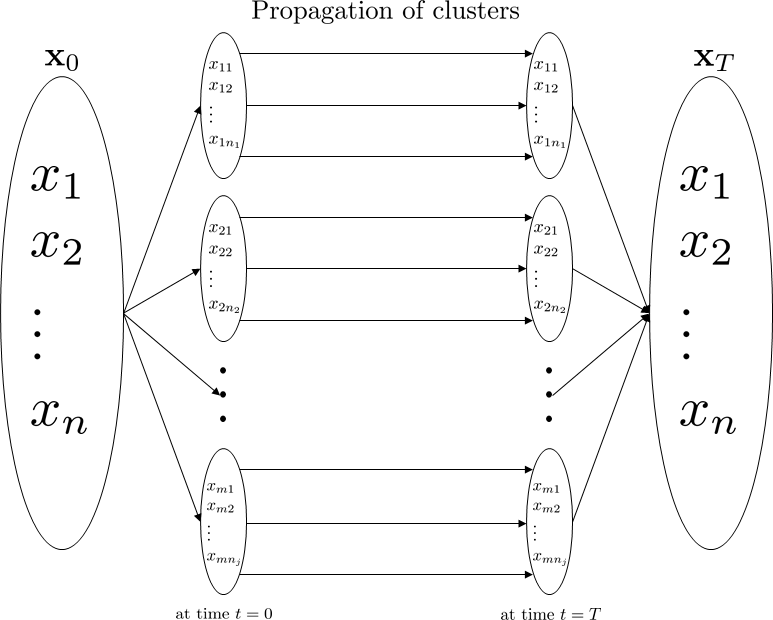
\includegraphics[scale=0.5]{figures_2/clusters}
\caption{Clustering of state variable and propagation of individual clusters in parallel}
\label{fig:clusters}
\end{figure}

Identification of WCSs is focused on the UQ of large-scale diffusively coupled dynamical systems. Given a stochastic nonlinear system with initial uncertainty information, it is desired to obtain the best possible linearized model to capture the interaction information among the state variables. Identification of WCSs is achieved through the use of standard graph decomposition techniques on the linearized system. When the number of interacting variables is large, it is prudent, if not imperative, to identify unique structural features in the form of WCSs. In contrast to the popular method of finding a Reduced Order Model (ROM)~\cite{wang2011two,carlberg2013gnat,matthies2003nonlinear,krack2013reduced}, whereby the dimension of the state space is transformed to canonical coordinates, the identification of WCSs can be easier, and the results can be easily interpreted. Additionally, the identified WCSs can often be of much lower dimension. These identified WCSs are considered to be decoupled from each other and thus can be analyzed independently. The UQ of WCSs can be carried out using existing highly efficient UQ methods.

This dissertation answers following questions concerning the identification of WCSs: i) What is the best possible linearization method? ii) How do we know, whether a large system can be decomposed into WCSs? iii)  What is an efficient clustering technique for such problems? Can any clustering technique be used? iv) How do we test the effectiveness of a clustering technique for the identification of WCSs? v)What is the physical interpretation of identified clusters? One of the critical contributions of this dissertation is to answer the questions mentioned above. Thus a vital focus of the dissertation is on the comparative study of different linearization and clustering techniques to enable proper system decomposition of diffusively coupled systems to facilitate smooth, faster, and effective UQ in large-scale nonlinear dynamical systems. 

In addition to answering the questions mentioned above, with respect to identification of WCSs, this dissertation makes following additional contributions:
\begin{enumerate}
\item Details of two novel time-domain Jacobian based linearization methods that can be used in the outlined framework is presented (Section~\ref{timedomain}).
\item A Jacobian-free state space linearization method that works well as part of the framework is also outlined (Section~\ref{stat_lin_section})
\item A novel method of permuting a sparse matrix into a block diagonal matrix % (Algorithm~\ref{alg1})
\item A novel metric to validate the utility of the discovered cluster structure is also presented (Section~\ref{wcs:num_exp}).
\end{enumerate}
There exist several measures to gauge the efficiency of clustering algorithms in case of static data. However, there is a need for developing a metric that can estimate the efficiency taking into consideration both the dynamics of the system and the evolution of uncertainty associated with each of the state variables. A novel metric has been proposed in this dissertation that not only considers the error between the state variables but also takes into account the uncertainty associated with each of the variables and the dynamics of the system. Additionally, a detailed comparative study is carried out to compare the performance of clustering techniques but also provides insights into the effects of different factors affecting the identification of suitable WCSs.

\subsection{Contribution 2:Identification of Strongly Connected Subsystems}


The second significant contribution of this dissertation relaxes the assumption of WCSs and focuses on the UQ of \textit{Strongly Coupled System} (SCS). In SCSs, a particular state variable is assumed to participate in more than one subsystems (Figure~\ref{clusters_2}). The concept of \textit{degree of participation} or fuzzy association of a state variable in a particular subsystem has been employed to enable UQ of high dimensional systems. The \textit{fuzzy association} allows us to determine the number of subsystems and the state variables participating in each subsystem. 

\begin{figure}[H]
\centering
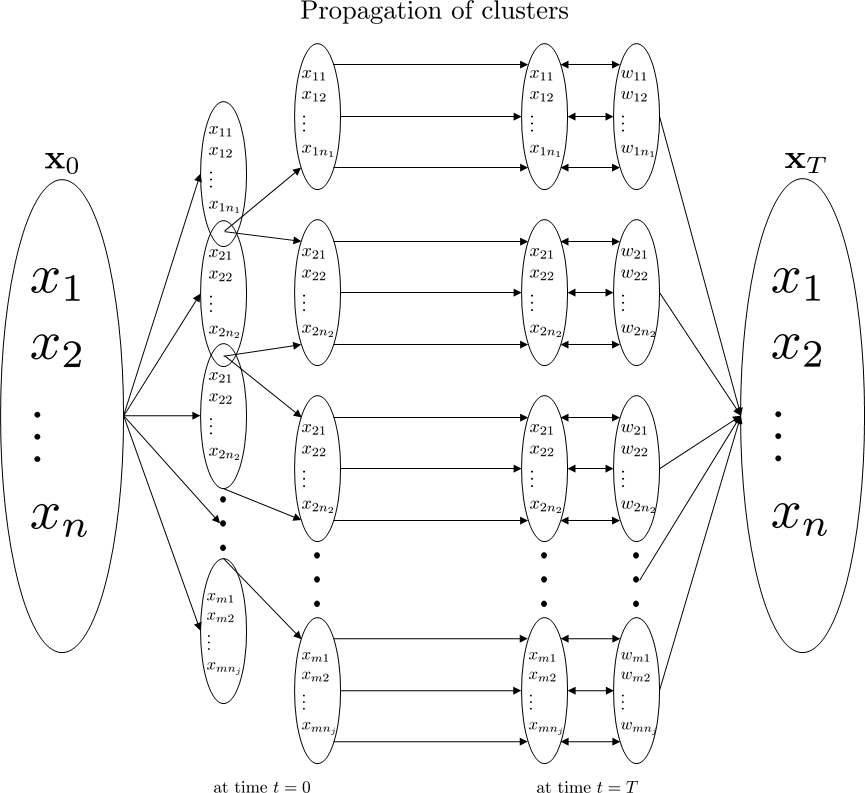
\includegraphics[scale=0.5]{figures_2/clusters_2}
\caption{Use of overlapping clusters of state variable for propagation of individual clusters in parallel. The third step shows mapping of overlapping variables to non-overlapping clusters.}
\label{clusters_2}
\end{figure}

Given a dynamical system with uncertainty information, the best possible linearization of the velocity function is approximated. The fuzzy association of the state variables in a particular subsystem is then obtained from an Overlapping Graph Clustering Algorithm. Such an algorithm treats linearized matrix as a well-connected graph and provides the number of clusters and the degree of participation of each node in a cluster. The clusters are propagated individually in parallel. Thereafter, the solution is obtained by the element-to-element or Hadamard product of the solution of the state variables in a cluster and their association in the cluster. 

Also, the idea of the two proposed frameworks has been extended to real-life applications. 
\begin{itemize} 
\item The WCS identification-based UQ method is applied to identify WCSs in a building energy model. Thermal networks can be modeled as a system of ODE comprising of a considerable number of state variables. The model is highly scalable depending on the size of the building. The researched model in question is derived from a real office/school building situated in Central New York. The building comprises of 132 thermal zones having very weak inter-zone interactions. The method is used to identify a zone or set of zones that behave independently.
\item The SCS identification-based UQ method is applied to generate random samples of a high-resolution Digital Elevation Model (DEM) in parallel in a geophysical mass flow problem. The governing equation is applied to the flow of hazards resulting from a volcanic eruption similar to the 1991 eruption in Volcan de Colima. The method is applied to detect SCS in the uncertain terrain profile of a $4.5 \text{km} \times 4.5 \text{km}$ region around Colima.
\end{itemize}


\section{Organization of the Dissertation}


To achieve the research challenges mentioned above and contributions, the dissertation is organized as follows:
Chapter~\ref{chap:uq} outlines the formulation of the problem and defines the concept of multidimensional integrals that are used for UQ in large dynamical systems. This formulation forms a foundation for the proposed frameworks outlined in the dissertation. It also reviews the existing UQ techniques and highlights the limitations of the current methods in solving high-dimensional uncertain systems.


Chapter~\ref{chap:wcs} discusses the concept of Weakly Connected Subsystems (WCS) in estimating the multidimensional integrals defined in Chapter~\ref{chap:uq}. Chapter~\ref{chap:wcs} also provides the background of linearization and focuses on identification of WCSs. Four methods of approximating a nonlinear system by a time-invariant linear system belonging to two different classes of \textit{Time-Domain} or \textit{Space-Domain} Linearization techniques are also detailed in Chapter~\ref{chap:wcs}. Chapter~\ref{chap:wcs} outlines the theoretical foundation and details of Spectral Clustering and Bayesian Non-negative Matrix Factorization clustering techniques that are used to identify WCS from the approximate linear system. Using the framework, the Chapter~\ref{chap:wcs} describes the set up for the filtering problem and their solutions. Finally, Chapter~\ref{chap:wcs} describes the numerical experiments and the test problems.


Chapter~\ref{chap:scs} extends the idea of WCSs to define Strongly Connected Subsystems (SCS) and provides the theoretical background for defining SCSs. Chapter~\ref{chap:scs} describes the concept of overlapping community detection techniques and reviews existing methods that apply to such problems. Chapter~\ref{chap:scs} also demonstrates how the linearization techniques described in Chapter~\ref{chap:wcs} can be used along with the overlapping community detection techniques to detect SCS. The effectiveness of the developed SCS framework is demonstrated on suitable numerical experiments. The numerical experiments include examples of coupled oscillators and a spatiotemporal flow problem defined by 1-D Shallow Water Model.  


Chapter~\ref{chap:building} utilizes the concept of WCS (Chapter~\ref{chap:wcs}) for optimal thermal load estimation in a large scale office building situated in Central New York. Chapter~\ref{chap:building} describes the building conditions, geometry, and the thermal properties of different components of the building. A physics based simplified model is described that uses the thermal properties to map the zonal temperatures, internal loads, and solar gains. Identification of WCSs is carried out on the developed model to carry out estimation of zonal temperatures, internal loads, and solar gains in a parallel fashion.


Chapter~\ref{chap:dem} performs effective UQ of hazard flow resulting from a volcanic eruption through the use of the SCS framework (Chapter~\ref{chap:scs}). The debris flow equation is solved over an uncertain terrain profile. It is shown how the SCS identification method can be used to sample realizations in parallel maintaining the same accuracy in estimation of the probabilistic hazard map. The methodology is used to perform the UQ resulting from a volcanic eruption in Volcan de Colima that occurred in 1991. 


Finally, Chapter~\ref{chap:conclusion} summarizes the main contribution of this dissertation and outlines the results and scope of future work. It also describes how the applicability of the developed framework can be extended to any high-dimensional scalable problems.  




























\chapter{Uncertainty Quantification in Dynamical Systems}
\label{chap:uq}

Consider a $n$-dimensional coupled dynamical system defined by the following Stochastic Differential Equation (SDE)
\begin{equation}
\label{stochdyn}
\dot{\mathbf{x}}_t = f(\mathbf{x}_t)  \hspace{5 mm} \textbf{x}_{t_0} = \textbf{x}_0
\end{equation}

\noindent where $\textbf{x} \in \mathbb{R}^n$ is the state variable, $f(x)$ is an $n$-dimensional vector of deterministic square integrable functions $f = [f_1,f_2,\ldots,f_n]$, with  $f: \mathbb{R}^n \times \mathbb{R}  \rightarrow \mathbb{R}^n$. Here $\mathbf{x}_t = \lbrace\mathbf{x}(t,\omega) , t \in [0,\infty) , \omega \in \Omega_{\mathbf{x}} \rbrace$ is a stochastic process defined on the probability space $(\Omega_\mathbf{x},\mathcal{F}_\mathbf{x},P_\mathbf{x})$ and
\begin{equation}
\textbf{x}_t :([0,\infty)\times \Omega_\mathbf{x}, \mathcal{B}([0,\infty)), \mathcal{F}_\mathbf{x}) \rightarrow (\mathbb{R}^n, \mathcal{B}(\mathbb{R}^n))
\end{equation}

Solution to Equation~\ref{stochdyn} admits is given by the nonlinear transformation $\textbf{x}_t = \phi^t(\mathbf{x}_0)$, where the deterministic flow is given by:
\begin{equation}
\label{stochflow}
\phi : \mathbb{R} \times \Omega_\mathbf{x}  \rightarrow \mathbb{R}^n
\end{equation}

Here the operation $\phi^t(x)$ is bijective, and satisfies (i) $\phi^0(\textbf{x}_0) = \textbf{x}_0$ and (ii) $\phi^{t+s}(\textbf{x}_0) = \phi^t(\phi^s(\textbf{x}))$, where $t \in \mathbb{R}$ is referred as time. Thus, the flow map $\phi^t(\mathbf{x}_0)$ is a random function depending on the initial distribution $\mathbf{x}_0$. 

\noindent In a given interval of time $t \in [0,T)$, a trajectory for a given initial condition $\textbf{x}_{0}$ at time $t = 0$ is defined as,

\begin{equation}
\label{gamma}
\gamma_{T,\textbf{x}_0} = \lbrace \phi^t(\textbf{x}_{0}) | t \in [0,T) \rbrace 
\end{equation}

\noindent An equilibrium point of the deterministic dynamical system with given flow velocity $f$, is defined as the point in the zero set of $f$ defined as,
\begin{equation}
\mathcal{Z} = \lbrace \tilde{x} \in \mathbb{R}^n | f(z) = 0 \rbrace
\end{equation}

The probability measure $P_{\textbf{x}_t}$ is characterized by the density function $p(\textbf{x}_t,t): \mathbb{R}^n \times \mathbb{R} \rightarrow [0,1]$ is a function of both $\textbf{x}_t$ and $t$, where,                     

\begin{equation}
\label{pdf_func}
P_{\textbf{x}_t} = P(\textbf{x}_t \leq \textbf{z}_t) = \int \int \ldots \int_{-\infty} ^{\textbf{z}_t} p(\tau,t) d\tau
\end{equation}

Our objective is to efficiently compute the statistical properties (say, first few moments) of state variable $\mathbf{x}_t = \phi^t(\mathbf{x}_0)$, given as:
\begin{equation}
\label{moments}
\begin{array}{l}
\mu_{t_k} = E[\mathbf{x}_{t_k}]  \\
\Sigma_{t_k} = E\left[(\mathbf{x}_{t_k} - \mu_{t_k})(\mathbf{x}_{t_k} - \mu_{t_k})'\right]
\end{array}
\end{equation}

\section{Moment Computation and Volume Integral}

\label{volume_integral}
As mentioned earlier, solution to system of high-dimensional ODEs requires solving simultaneous high-dimensional integrals. Let us consider an ODE $\dot{\textbf{x}}_t = f(\textbf{x}_t)$, $\textbf{x} \in \mathbb{R}^n$, represented by vector of deterministic functions $f = [f_1,f_2,\ldots,f_n]$, where $f_i:\mathbb{R}^n \rightarrow \mathbb{R}$, $i = 1$ to $n$. Similar to Equation~(\ref{stochflow}), the solution to this equation is given by the vector of functions $\phi^t(\textbf{x}_0) = [\phi^t(\textbf{x}_0)_1, \phi^t(\textbf{x}_0)_2, \ldots, \phi^t(\textbf{x}_0)_n]$, where $\textbf{x}_0$ is the initial condition. The solution $\textbf{x}_t = \phi^t(\textbf{x}_0)$ is defined for all $t \in \mathbb{R}$. The function $\phi^t(\textbf{x}_0)$ is obtained by solving the system of integral given as,

\begin{equation}
\label{integral_whole}
\mathbf{x_{t}} =  \phi^t(\mathbf{x}_0) = \mathbf{x}_0 + \int_0^t f(x_{\tau 1},x_{\tau 2},\ldots,x_{\tau n}) d \tau
\end{equation}

\noindent and the moment of an arbitrary function $\mathcal{G}$ similar to Equation~\ref{moments} can be written using the following volume integral,

\begin{equation}
\label{moment_whole}
E[\mathcal{G}(\textbf{x}_t)] = \int \int \ldots \int_{\Omega_{\textbf{x}}} \mathcal{G}(x_{t1},x_{t2},\ldots,x_{tn}) dP_{\textbf{x}}
\end{equation}


\section{Methods of Uncertainty Quantification}

UQ in high-dimensional dynamical systems involves propagation and computation of complex stochastic integrals involving the state variables. An analytical expression for the integrals in Equation~\ref{moment_whole} exists for only a few pdfs for a limited number of transformations. For arbitrary nonlinear transformations (such as Equation~\ref{integral_whole}), usage of numerical UQ techniques become the only possible solution. Any UQ method utilizes the definition of the pdf to generate sample points to compute the integral equation (Equation~\ref{integral_whole}). UQ methods studied in this dissertation is classified into two types: (i) Sampling-based methods and (ii) Collocation based methods. Given below is a review of some of the existing UQ methods. Review of Polynomial Chaos Expansion~\cite{xiu2002wiener} and related Galerkin projection methods~\cite{fletcher1984computational} are beyond the scope of this dissertation. 


\section{Monte Carlo Integration}

Integral computation as in Equation~\ref{moment_whole} can be based on random sampling or Monte Carlo (MC) sampling $\mathcal{X}_i$ of the pdf $p_\textbf{x} = dP_\textbf{x}$ and computation of the function value $\mathcal{G}(\mathcal{X}_i)$ for each random sample~\cite{fishman1996monte}. If there are $\mathcal{N}$ number of random samples, then Equation~\ref{moment_whole} can be computed as,

\begin{equation}
\label{monte_int}
E[\mathcal{G}(\textbf{x}_t)] = \int \int \ldots \int_{\Omega_{\textbf{x}}} \mathcal{G}(x_{t1},x_{t2},\ldots,x_{tn}) dP_{\textbf{x}} = \frac{
1}{\mathcal{N}} \sum_i^{\mathcal{N}} \mathcal{G}(\mathcal{X}_i)
\end{equation}

The integral in Equation~\ref{monte_int} is also referred to as Monte Carlo integral equation. The pdf $p_{\textbf{x}_t}(\bm{\tau})$ at any time $t$ is estimated from the evolution of the samples $\mathcal{X}_i$ via the propagation equations~\ref{stochdyn} and~\ref{stochflow}. Figure~\ref{montecarlo} shows a schematic of Monte Carlo based UQ method applied on an ODE. 

\begin{figure}[H]
\begin{center}
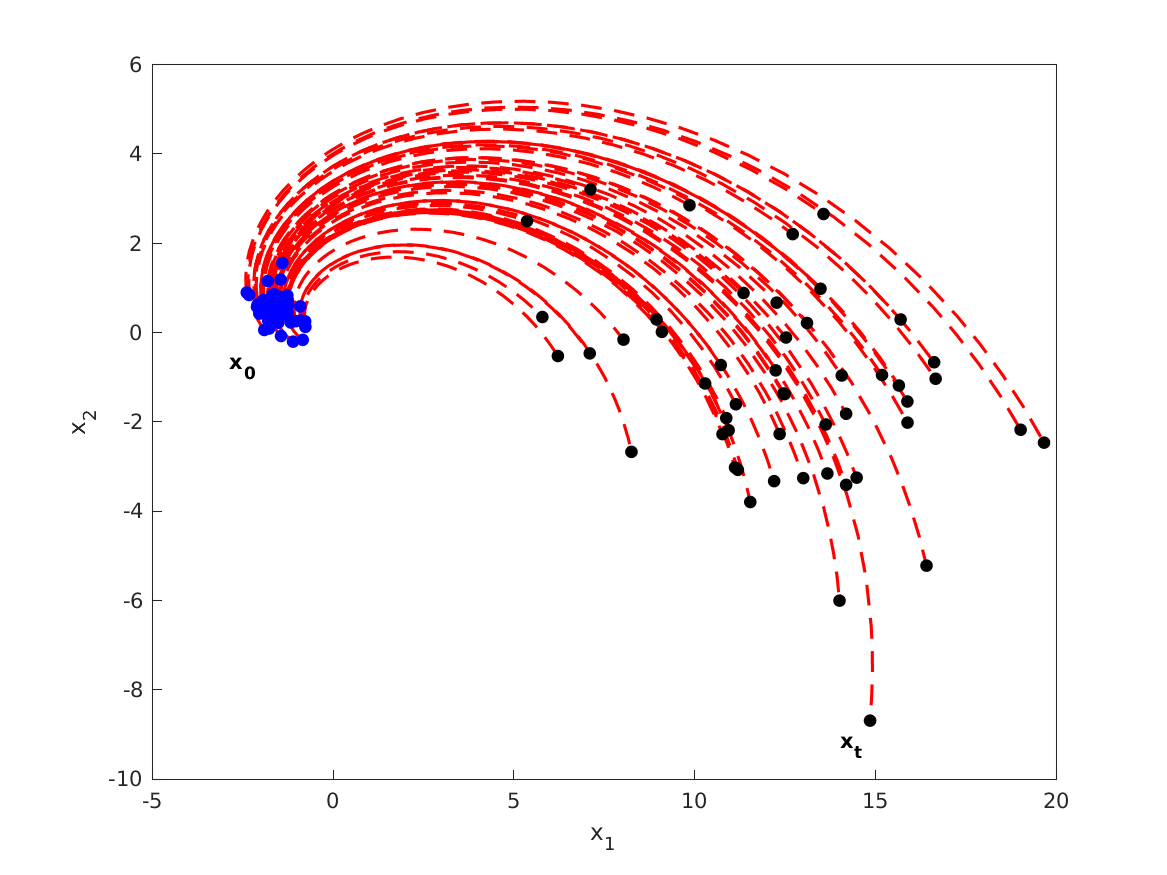
\includegraphics[scale=0.5]{figures/montecarlo}
\caption{Schematic of Monte Carlo simulation based UQ method applied on an ODE}
\label{montecarlo}
\end{center}
\end{figure}


The number of samples $\mathcal{N}$ and associated accuracies depends on the type of sampling methods employed. Standard sampling techniques refer to the generation of pseudo-random numbers. However, the convergence rate of the integral Equation~\ref{monte_int} can be estimated using the Central Limit Theorem as~\cite{stroud1971approximate} 

\begin{equation}
\epsilon_{\mathcal{N}} = \left(\frac{E[f^2]- E[f]^2}{\mathcal{N}}\right)^{1/2} 
\end{equation}

Figure~\ref{fig:monte_accuracy} shows the accuracy of MC sampling from an $n$-dimensional Gaussian random variable. The increase in estimation error shows a linear pattern with $n$. To reduce the error in convergence, different variance reduction techniques have been developed. These techniques use an underlying MC method and employ other deterministic techniques such as stratification, low discrepancy sequence generation to reduce the error in convergence. 


\begin{figure}[H]
\centering
\begin{subfigure}{0.45\textwidth}
\centering
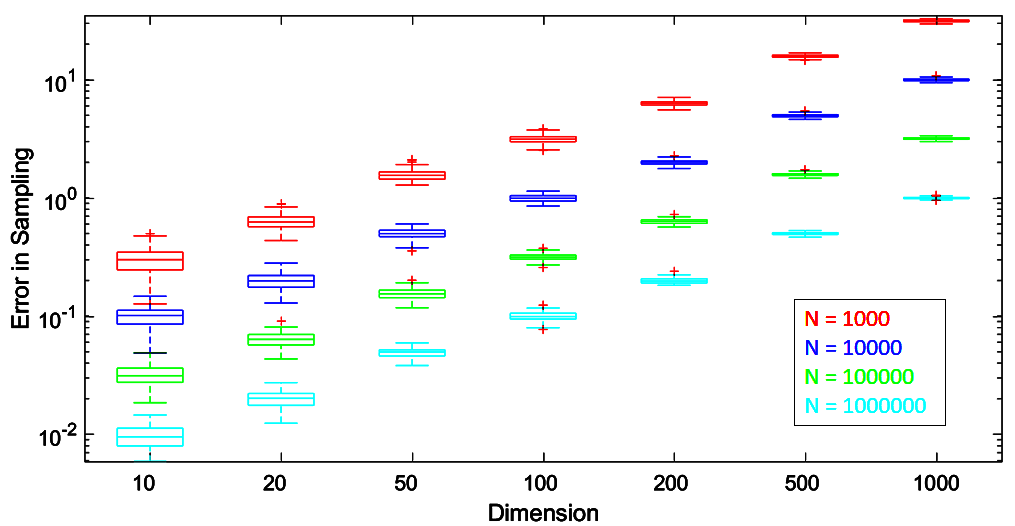
\includegraphics[width=\textwidth]{uq_figs/monte_log}
\caption{}
\end{subfigure}
\begin{subfigure}{0.45\textwidth}
\centering
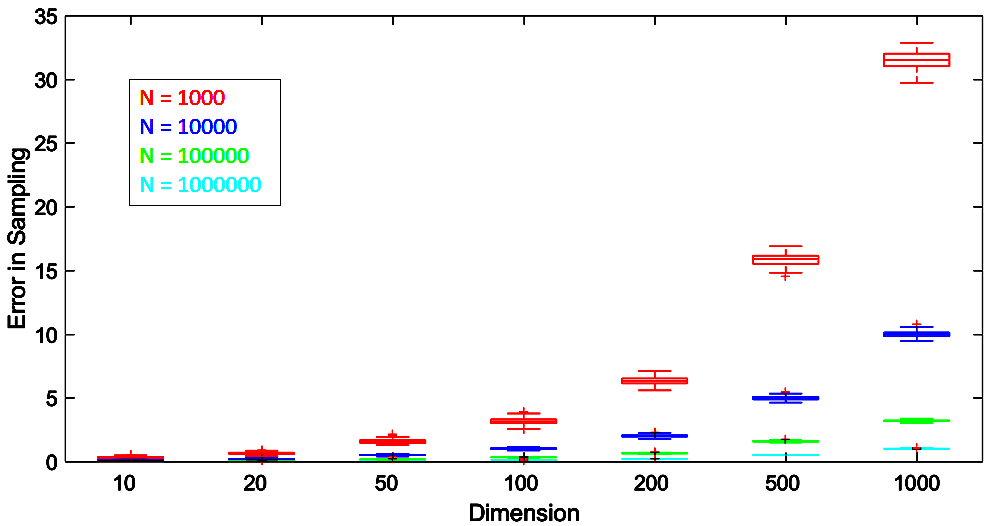
\includegraphics[width=\textwidth]{uq_figs/monte_linear}
\caption{}
\end{subfigure}
\caption{Error in Sampling by Monte Carlo sampling with dimension $n$ on (a) log scale and (b) linear scale}
\label{fig:monte_accuracy}
\end{figure}

%such as Monte Carlo Simulation~\cite{fishman1996monte}, Importance Sampling~\cite{melchers1989importance}, Quasi-Monte Carlo simulation~\cite{caflisch1998monte} 


% or quadrature based techniques such as Gaussian Quadrature~\cite{stroud1966gaussian}, Cubature~\cite{arasaratnam2009cubature}, Polynomial Chaos Expansion (PCE)~\cite{xiu2002wiener} may require huge amount of computation time, depending on the dimension of the problem. 

\begin{table}[H]
\begin{center}
\caption{List of some standard UQ methods}
\resizebox{\columnwidth}{!}{
\label{uq_methods}
\begin{tabular}{|l|l|l|}
\hline
Sampling-Based Methods& Examples \\ \hline
MC (pseudo-random number generator) &   Mersenne Twister~\cite{matsumoto1998mersenne}, LCG~\cite{marsaglia1972structure}, LFG~\cite{marsaglia1990toward} \\ \hline
Low-Discrepancy (Quasi-MC) &   Halton~\cite{halton1960efficiency}, Hammersley~\cite{hammersley2013monte}, Sobol~\cite{bratley1988algorithm}, van der Corput~\cite{der1935verteilungsfunktionen} \\ \hline
Stratified Sampling & LHS~\cite{iman2008latin} \\ \hline
Markov Chain MC Sampling & Metropolis-Hastings~\cite{hastings1970monte}, Gibbs~\cite{geman1984stochastic}, HMC~\cite{duane1987hybrid} \\ \hline
Other &  Importance Sampling~\cite{melchers1989importance} \\ \hline
\end{tabular} 
}
\end{center}
\end{table}

However, since all sampling methods are derived from the traditional Monte Carlo sampling, the linear accuracy trends for all of them are similar. 

\section{Quadrature-based Methods}

Quadrature (or Cubature for number of dimensions more than one) based methods involve a deterministic scheme to generate the set of $\mathcal{N}$ collocation points $\mathcal{X}_i$'s and associated weights $W_i$'s, such that the expectation integral in Equation~\ref{moment_whole} can be formulated as,

\begin{equation}
\label{quad_int}
E[\mathcal{G}(\textbf{x}_t)] = \int \int \ldots \int_{\Omega_{\textbf{x}}} \mathcal{G}(x_{t1},x_{t2},\ldots,x_{tn}) dP_{\textbf{x}} =  \sum_i^{\mathcal{N}} \mathcal{W}_i \mathcal{G}(\mathcal{X}_i)
\end{equation}

Setting all $W_i = 1/\mathcal{N}$ gives you Equation~\ref{monte_int}. However, unlike the MC methods, quadrature-based methods do not rely on any pseudo-random number generator. Instead, they use different classes of orthogonal polynomials to generate $(\mathcal{X},\mathcal{W})_i$'s via quadrature rule. The 1-D quadrature rule~\cite{stroud1966gaussian} states that, by suitably choosing suitable pair of $(\mathcal{X},\mathcal{W})_i$'s, the following 1-D integral equation can be solved exactly up to a polynomial degree of $2\mathcal{N} - 1$

\begin{equation}
E[g(x)] = \int_{\Omega_{x}} g(x) dP_x = \sum_i^{\mathcal{N}} g(\mathcal{X}_i) \mathcal{W}_i
\end{equation}

\noindent Setting $g(x) = \lbrace 1,x,x^2,\ldots,x^{2\mathcal{N} - 1} \rbrace$ the above equation becomes the 1-D moment constraint equation (MCE) as,

\begin{equation}
\label{mce_1d}
Q_d = E[x^d] = \int_{\Omega_x} \tau^d p_x(\tau) d \tau = \sum_i^{\mathcal{N}} \mathcal{X}_i^d \mathcal{W}_i \hspace{5mm} d = 0,1,\ldots,2\mathcal{N} - 1
\end{equation}

Instead, of solving the system of equations in~\ref{mce_1d}, the weight functions are assumed to belong to a suitable class of orthogonal polynomial of order $\mathcal{N}$. It can be shown that the collocation points $\mathcal{X}_i$'s are the roots of the particular $\mathcal{N}$-th order polynomial~\cite{press2007numerical}. The choice of this polynomial depends on the class of pdf involved in Equation~\ref{mce_1d} (For example use of Hermite polynomial for Gaussian pdf). Abramowitz and Stegun~\cite{abramowitz1964handbook} have listed a list of orthogonal polynomials (see Table~\ref{gauss_quad_pol}) and their roots. 

\begin{table}[H]
\begin{center}
\caption{1D Gauss Quadrature polynomials}
\label{gauss_quad_pol}
\resizebox{\textwidth}{!}{
\begin{tabular}{|c|c|c|c|}
\hline
$\Omega$ & Orthogonal Polynomial & Function & Quadrature Rule \\ \hline
$(-\infty,+\infty)$ & Hermite & $\exp(-x^2)$ & Gauss-Hermite \\ \hline
$[-1,1]$ & Legendre & $1$ & Gauss-Legendre \\ \hline
$[0,+\infty)$ & Laguerre & $x^a \exp(-x) $ & Gauss-Laguerre \\ \hline
$[-1,1]$ & Chebyshev & $1/\sqrt{1-x^2}$ & Gauss-Chebyshev \\ \hline
$[-1,1]$ & Jacobi & $(1-x^a)(1+x^b), a,b > -1 $ & Gauss-Jacobi \\ \hline
\end{tabular}
}
\end{center}
\end{table}

Cubature method (quadrature for $n>1$) is an extension of the 1-D Gaussian quadrature method, whereby instead of solving the 1D MCE in Equation~\ref{mce_1d}, the pair of collocation points and weights $(\mathcal{X},W)_i$'s can exactly produce moments of a multivariate polynomial functions up to order $d$, by solving the following n-dimensional MCE:

\begin{equation}
\label{mce_nd}
Q_d^n = \sum_{i=1}^{\mathcal{N}_d} w_i \lbrace x_1^{m_1} \ldots x_n^{m_n} \rbrace = E \left[ x_1^{m_1},\ldots,x_n^{m_n}  \right]  \hspace{5mm} m_1 + m_2 + \ldots m_n \leq d
\end{equation}

\subsection{Gaussian Cubature}

Gaussian cubature~\cite{arasaratnam2009cubature}, also termed as product rule is generated by taking the tensor product of the 1D quadrature rule explained above. Given a multivariate pdf $p(\textbf{x}) = \lbrace x_1, \ldots, x_n \rbrace$, $\textbf{x} \in \mathbb{R}^n$, the first step is to generate $\mathcal{N}$ collocation points and weights $(\mathcal{X}_j,\mathcal{W}_j)_i$ for each variable $x_J$ to approximate polynomial integral up to degree $2\mathcal{N} - 1$. Next, the set of collocation points for $\textbf{x}$ is generated by taking the tensor product of all $\mathcal{X}_j$ set of points by the following integral equation

\begin{equation}
\label{eqn:gauss_quad}
Q_d^n = Q_d^1 \otimes Q_d^2 \otimes \ldots \otimes Q_d^n
\end{equation}

Thus the number of points generated is $\mathcal{N}_n = \mathcal{N}^n$. The associated weights are formulated as,

\begin{equation}
W_i = W_{1i}W_{2i} \ldots W_{ni} \ldots i = 1,2,\ldots,\mathcal{N}_n
\end{equation}

It is evident that this method suffers from the curse of dimensionality as the required number of points grows exponentially with the dimension $n$ (see Figure~\ref{fig:gauss_quad} for a given value of $d$ as per Equation~\ref{mce_nd}. 

\begin{figure}[H]
\centering
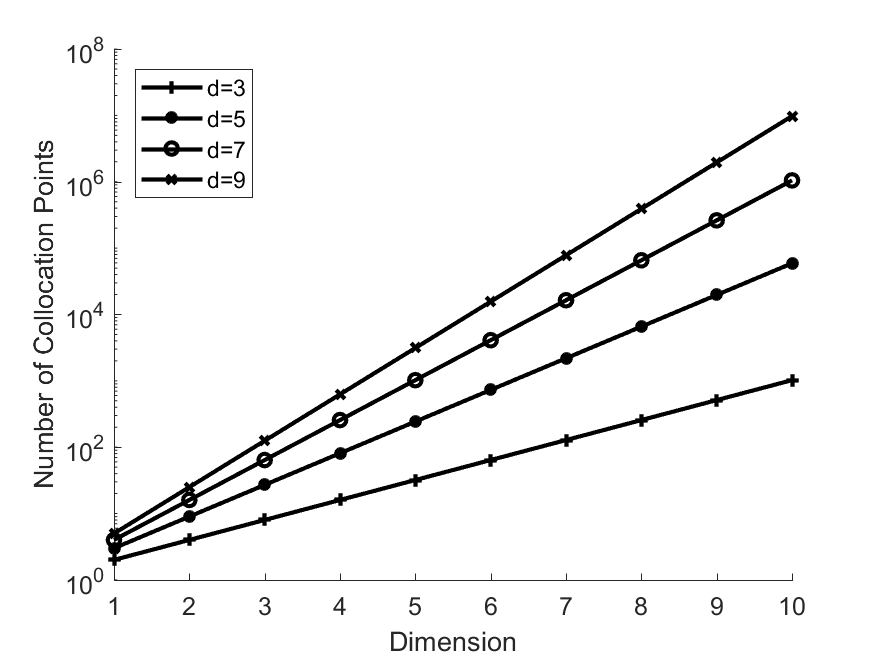
\includegraphics[width=\textwidth]{intr_figs/gauss_hermite}
\caption{Number of Collocation Points vs Dimension $n$ for different values of $d$ in Equation~\ref{mce_nd} using Gauss-Hermite class of Orthogonal Polynomial}
\label{fig:gauss_quad}
\end{figure}


\subsection{Sparse-Grid Collocation}

Sparse-Grid or Smolyak collocation techniques generates the cubature rule by invoking a sparse tensor product unlike the Gaussian cubature to reduce the number of monomials involved in the integral calculation of Equation~\ref{monte_int}. The number of monomials involved in Equation~\ref{eqn:gauss_quad} is $\binom{n+d}{n}$ that grows exponentially with $n$ for a given $d$. Smolyak observed that the key to reducing the number of collocation points lie in the number of monomials involved for the integral computation. The first step of generating collocation points is similar to 1D quadrature method of solving Equation~\ref{mce_1d}. The integral equation in~\ref{mce_nd} for a given $d$ can be written in a recursive formulation as~\cite{gerstner1998numerical},

\begin{equation}
\label{mce_sparse}
Q_k^n = \sum_i^k (Q_i^1 - Q_{i-1}^1) \otimes Q^{n-1}_{k-i+1} 
\end{equation}

\noindent where, $d=2k-1$, $Q_n^1$ is the univariate quadrature rule and $Q_0^1 = \emptyset$. Under this transformation in Equation~\ref{mce_sparse}, the number of collocation points comes out to be less than that required by the product in Equation~\ref{eqn:gauss_quad}. However, the required number of collocation points still grows exponentially with the size of the problem (see Figure~\ref{fig:gauss_quad_sparse}). 

\begin{figure}[H]
\centering
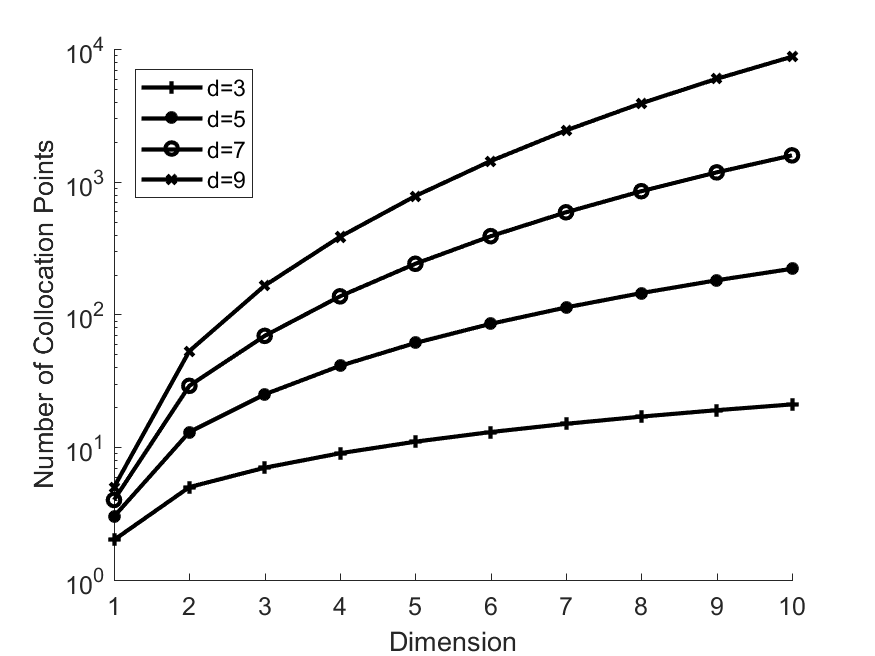
\includegraphics[width=\textwidth]{intr_figs/gauss_hermite_sparse}
\caption{Number of Collocation Points vs Dimension $n$ for different values of $d$ in Equation~\ref{mce_sparse} using Gauss-Hermite class of Orthogonal Polynomial}
\label{fig:gauss_quad_sparse}
\end{figure}

\subsection{Minimal Cubature Rules}

For faster computation of the integral Equation~\ref{mce_nd} maintaining the same exactness, cubature rules have been proposed that optimally chooses the number of collocation points $N$ depending on $n$, $d$, choice of the pdf $p(x)$ and also the domain of integral $\Omega_{\textbf{x}}$. A list of minimal cubature rules can be listed in Refs~\cite{stroud1971approximate,cools2003encyclopaedia,Cools1}. Readers are also advised to check Ref~\cite{cubatureurl} for tabulated form of different cubature rules along with their references. An excerpt of the table for Gaussian weight function is given in Table~\ref{tab:cubature}.

\begin{table}
\begin{center}
\caption{Cubature formula with weight function $\exp(-\textbf{x}^T\textbf{x})$, $\textbf{x} \in \mathbb{R}^n$}
\label{tab:cubature}
\begin{tabular}{|c|c|c|}
\hline
$d$ & $N$ & $n$ \\ \hline
3  & $2n$ & all dimensions \\ \hline
3  & $2^n$ & all dimensions \\ \hline
5  & $n^2 + n + 2$ & $2 \leq n \leq 7$ \\ \hline
5  & $2^{n+1} - 1$ & all dimensions \\ \hline
7  & $2^n + 2n^2 + 1$ & $3 \leq n \leq 7$ \\ \hline
7  & $ ( 4n^3 + 12n^2 - 4n + 3 ) / 3$ & all dimensions \\ \hline
9  & $( 2n^4 - 4n^3 + 22n^2 - 8n + 3 ) / 3$ & $n \geq 4$ \\ \hline
11  & $( 4n^5 - 20n^4 + 140n^3 - 130n^2 + 96n + 15 ) / 15$ & all dimensions \\ \hline
\end{tabular}
\end{center}
\end{table}

\subsection{Unscented Transform}

Unscented Transform~\cite{julier1997new} is fast and accurate UQ method for problems with Gaussian variables. Given, at a time instance, the state variable $\mathbf{x}_{t_k}$ is Gaussian, UT generates sample points $\mathcal{X}_i$ and associated weights $W_i$ that can accurately estimate the moments of the Gaussian variable up to the order 2. In other words, the sample points $\mathcal{X}_i$ satisfy the moment constraint equations given in Equation~\ref{mce_nd}. Here, $m_1 + m_2 + \ldots m_n = 2$. Given the distribution of $\textbf{x}_t \sim \mathcal{N}(\bm{\mu}_{t_k},\Sigma_{t_k})$, UT uses a deterministic technique to generate the sigma points $\mathcal{X}$ and the related weights $W$ as~\cite{julier1997new}:
\begin{equation}
\label{sigmapt}
\begin{array}{lr}
\mathcal{X}_0 = \bm{\mu}_{t_k} &W_0 = \kappa /(n+ \kappa)  \\
\mathcal{X}_i = \bm{\mu}_{t_k} + \left( \sqrt{(n+ \kappa) \Sigma_{t_k}} \right)_i  &W_i = 1 /2(n+ \kappa)  \\
\mathcal{X}_{i+n} = \bm{\mu}_{t_k} - \left( \sqrt{(n+ \kappa) \Sigma_{t_k}} \right)_i  &W_{i+n} = 1 /2(n+ \kappa)
\end{array}
\end{equation}
$\left( \sqrt{(n+ \kappa) \Sigma_{t_k}} \right)_i$ is the $i$th row or column of the matrix square root of $(n+ \kappa) \Sigma_{t_k}$. For the numerical examples, the value of $(n+\kappa)$  has been taken to be 3. These sigma points are then propagated by the flow map $\phi^t(\mathcal{X})$ as defined in Eqn.~\ref{stochflow}. The mean and the variance of the propagated points at time $t_{k+1}$ is given by,
\begin{equation}
\label{prop}
\begin{array}{l}
\bm{\mu}_{t_{k+1}} =  \displaystyle \sum_{i=1}^{2n+1} W_i \mathcal{X}_i   \\
\Sigma_{t_{k+1}} = \displaystyle \sum_{i=1}^{2n+1} W_i (\mathcal{X}_i - \bm{\mu}_{t_{k+1}})(\mathcal{X}_i - \bm{\mu}_{t_{k+1}})^T  \notag
\end{array}
\end{equation}
\begin{figure}[H]
\centering
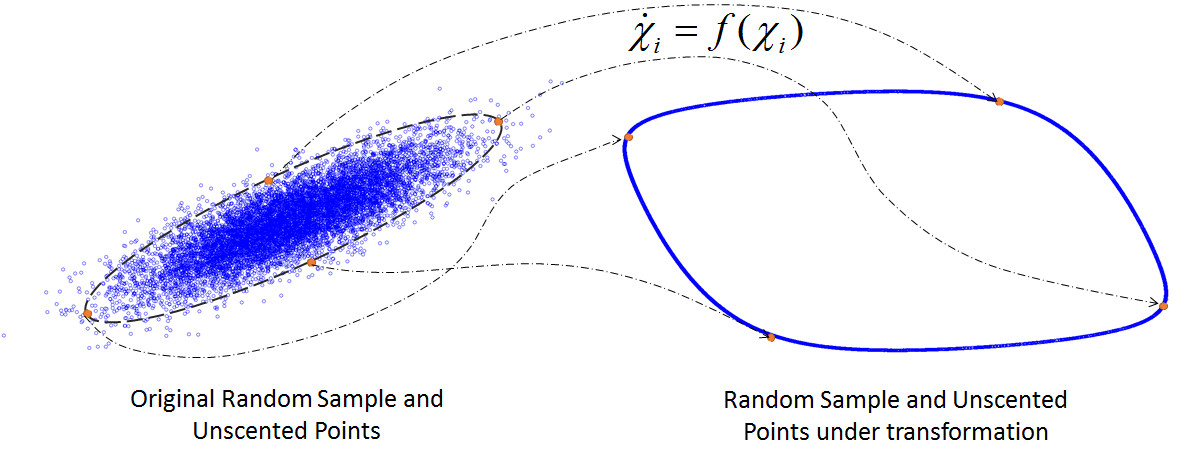
\includegraphics[width=\textwidth]{figures/FIG_9}
\caption{Working of the Unscented Transformation}
\label{UnscT}
\end{figure}

Figure~\ref{UnscT} shows the analogy between Monte-Carlo samples and UT sigma points, which are generated from the initial distribution space and then are propagated through the dynamical flow equation.

\subsection{Other Methods}

Prior work related to Uncertainty Quantification (UQ) in nonlinear systems is mostly limited to efficiently solving small-scale problems~\cite{mezic2008uncertainty,demars2013entropy,fujimoto2012analytical}. For large scale systems, UQ methods based on decoupling entire state space into interconnected smaller state spaces 
have been recently pursued~\cite{callier1976input,georgiou1992linear,varigonda2004graph,dellnitz2003congestion,surana2012iterative}. A fundamental limitation of these existing works is the approximation of the nonlinear nature of the system through the use of Jacobian at the initial condition.

A summary of all the methods show that, it is hard to obtain a method that works for any degree $d$ and for any dimension $n$. Product-rule based Gaussian cubature and Smolyak-grid collocation method shows exponential requirement of collocation points. The cubature rules in Table~\ref{tab:cubature} exist for certain dimension $n$ and for any degree of polynomial approximation $d$. Linear requirement of collocation points $N$ exist only for $d=3$. For other $d$'s, $N$ varies either in polynomial or exponential order. Such a requirement can scale up fast for high-dimensional problems.
Despite the effectiveness, the approaches mentioned above still requires significant computation time while tackling scalable high-dimensional problems. For such methods, it is imperative to incorporate a clustering method with any of the UQ techniques, to achieve the same efficiency for a lesser computational time. 
\chapter{Identification of Weakly Connected Subsystems (WCSs) for Effective UQ}
\label{chap:wcs}


\section{Proposed Framework for Identification of WCSs}
\label{framework}

In this section, the key features of the proposed framework for the analysis of a stochastic dynamical system and identifying WCSs is discussed. The main idea is to approximate the large dynamical system as multiple weakly connected low-dimension systems~\ref{fig:clusters}. This concept allows us to solve multiple low-dimension problems rather than one large dimension problem. 

\begin{figure}[H]
        \centering
        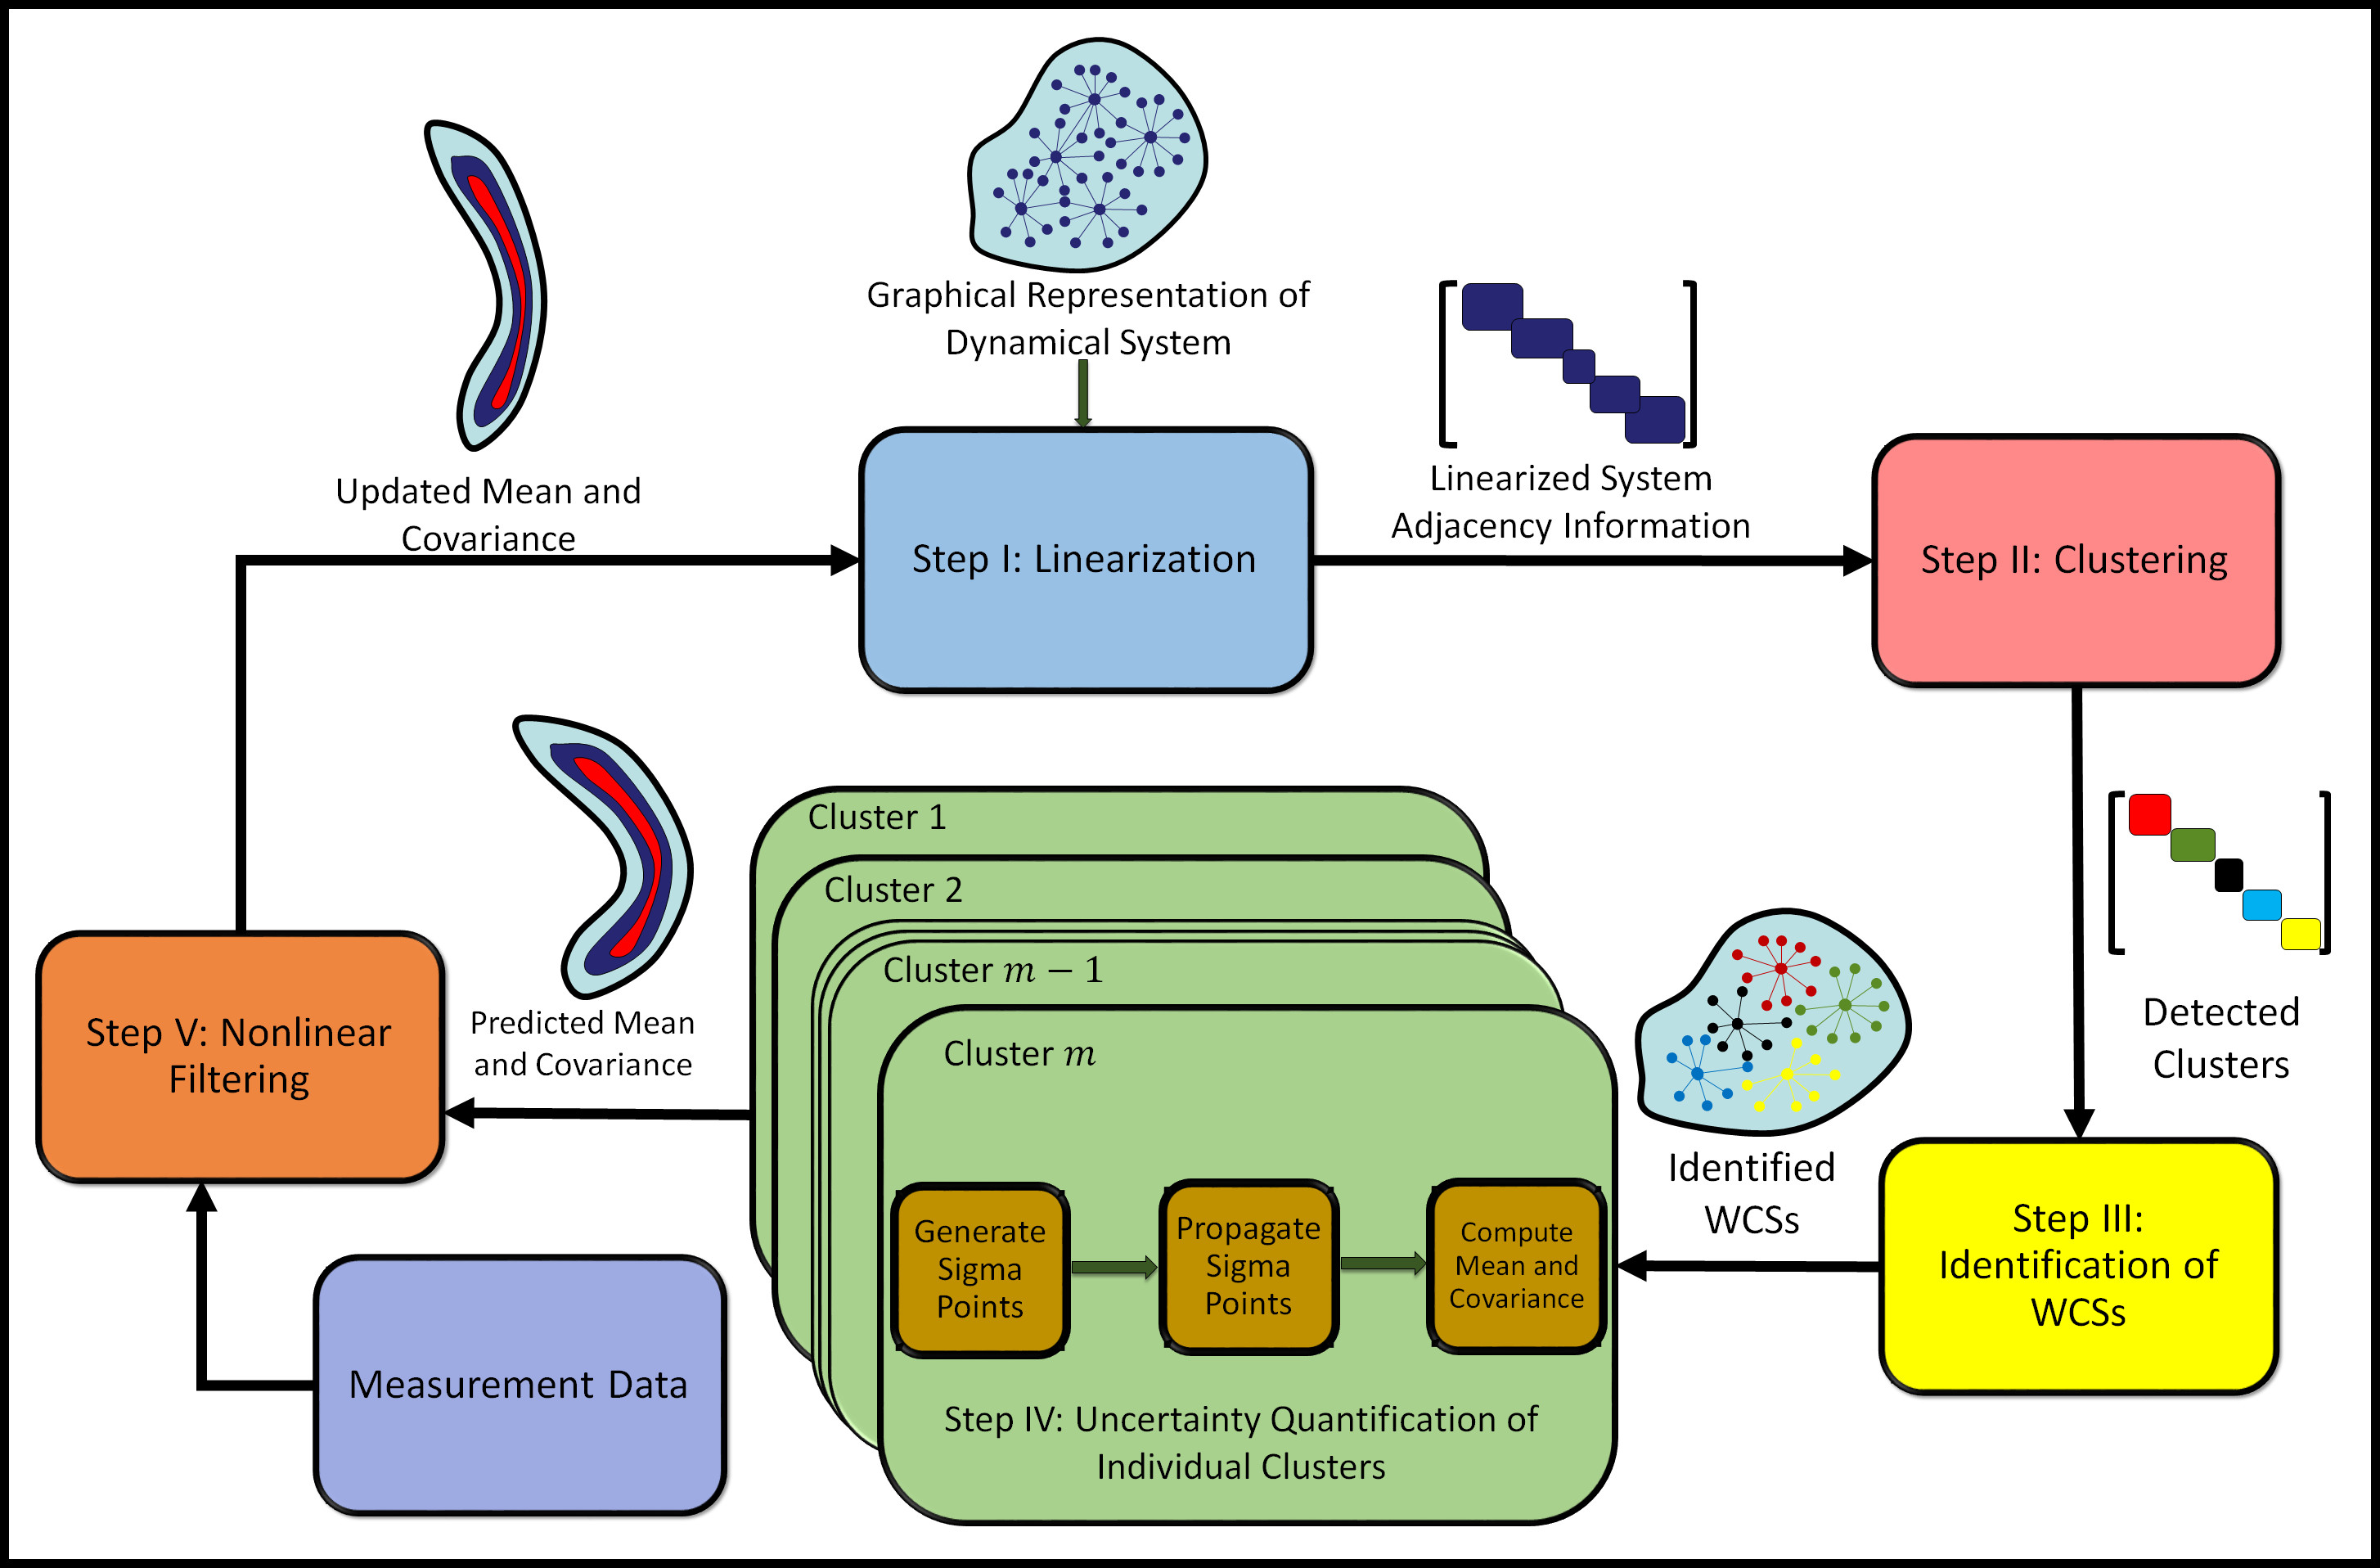
\includegraphics[width=0.8\textwidth]{figures/FIG_2}
        \caption{Determination of Weakly Coupled Subsystems (WCSs): Flowchart explaining the framework for linearization and clustering procedure followed by effective UQ}
        \label{fig:UQframework_2}
\end{figure}

Figure~\ref{fig:UQframework_2} shows the different components of the overall framework. Given a dynamical system with uncertainty in the initial condition, a graph-theoretic representation (as an undirected graph) of the dynamical system is used, where the state variables represent the vertex of the graph. We hypothesize, the graph to be consisting of strongly connected components (or variables) connected by weak edges. These weak edges in conjunction with the clustering methods are used to identify the WCSs. The adjacency or edges in graphical representation are derived from the linear approximation of time derivative of the state vector about the nominal point. In this respect, the first step is to linearize the large dimensional state space in a domain of interest using time and space domain linearization methods. The linearization step helps in quantifying the connectivity information among different state variables (nodes of the graph). The resulting linear system matrix stores the weighted graph adjacency information. Once the graph adjacency matrix is derived from the linearization process, the graph clustering methods are used to identify the clusters in the connected graphs. The next step involves identification of the WCSs. These WCSs are identified by mapping the individual clusters or blocks in the weighted adjacency graph to the state variables involved. The variables of each WCS are used to create the clustered model. The uncertainty quantification methods exploit the identified WCS to propagate the state statistical moments through each WCS, which are updated on the availability of the measurement data. The updated statistical moments are used to define the domain of interest to recompute the adjacency matrix for the clustering methods. Hence, the overall framework is a data-driven cyclic process which goes back to the first step after recalibrating the statistical properties of the state variables on the availability of the data. In subsequent subsections, the details corresponding to the primary steps involved in the proposed framework is outlined.

\section{Weakly Connected Subsystems}

Weakly Connected Subsystems or WCSs are defined as subsystems of the large state space $\mathbf{x}_t \in \mathbb{R}^n$ such that they are approximately decoupled with each other, and their ensemble can approximately replicate the dynamics of the whole system. Mathematically speaking, given the initial value problem defined in Chapter~\ref{chap:uq}, the state space $ \textbf{x}_t \in \mathbb{R}^n$, is clustered into:
\begin{equation}
\label{clustmodel}
\begin{array}{l}
\mathbf{y}_{t_1} = \lbrace x_{t_{11}},x_{t_{12}},\ldots,x_{t_{1n_1}} \rbrace  \\
\mathbf{y}_{t_2} = \lbrace x_{t_{21}},x_{t_{22}},\ldots,x_{t_{2n_1}} \rbrace  \\
\vdots  \\
\mathbf{y}_{t_m} = x_{t_{m1}},x_{t_{m2}},\ldots,x_{t_{mn_1}} \rbrace 
\end{array}
\end{equation}

Where, $\sum_{j=1}^m n_j = n$. Each subset $\mathbf{y}_{t_j} \in \textbf{x}_t$, $j = 1$ to $m$ is termed as a WCS. Each subsystem $\mathbf{y}_{t_j}$ is thus modeled by the ODE defined in $\mathbb{R}^{n_j}$ as 

\begin{equation}
\label{substochdyn}
\dot{\mathbf{y}}_{t_j} = f(\mathbf{y}_{t_j}) \hspace{5 mm} j = 1,2,\ldots,m
\end{equation} 

\noindent The solution is approximated as

\begin{equation}
\label{integral_wcs}
\mathbf{y}_{t_j} =   \mathbf{y}_{t_j} + \int_0^t f(x_{\tau_{j1}},x_{\tau_{j2}},\ldots,x_{\tau_{jn_j}}) d \tau
\end{equation}

\noindent and the moment equation is computed from the reduced order volume integral given as,

\begin{equation}
\label{moment_wcs}
E[\mathcal{G}(\mathbf{y}_{t_j})] = \int  \int \ldots \int_{\Omega_{j \textbf{x}}} \mathcal{G}(x_{t_{j1}},x_{t_{j2}},\ldots,x_{t_{jn_j}}) dP_j
\end{equation}

\noindent where, each random vector $\mathbf{y}_{jt}$, $j = 1,\ldots,m$ is defined on the probability space $(\Omega_{j \textbf{x}},\mathcal{F}_{j \textbf{x}},P_j)$, such that $\Omega_{\textbf{x}}$ is the disjoint union of the countable partitions $\Omega_{j \textbf{x}}$'s. Thus: 
\begin{equation}
\begin{array}{l}
\Omega_{\textbf{x}} =  \displaystyle \bigcup_{j=1}^m \Omega_{j \textbf{x}}  \\
\mathcal{F}_{\textbf{x}} = \mathcal{F}_{1\textbf{x}} \times \mathcal{F}_{2 \textbf{x}} \times \ldots \times \mathcal{F}_{m \textbf{x}} \\
P_{\textbf{x}} = P_1 \times P_2 \times \ldots \times P_m
\end{array}
\end{equation}
Also,
\begin{equation}
P(A_j,A_k) = P(A_j)P(A_k) \text{ for } A_j \in \mathcal{F}_j,A_k \in \mathcal{F}_k, \;\forall \; j \neq k
\end{equation}

Such an approximation can benefit any numerical technique, both deterministic and probabilistic. Instead of solving for the whole system, one can solve for the WCSs $\dot{\mathbf{y}}_{t_j} = f(\mathbf{y}_{t_j})$ in parallel. Now, the theoretical formulation of linearization and clustering that facilitates the identification of WCSs in a high-dimensional nonlinear stochastic system is described in details. 

\section{Approximate Linearization of Nonlinear System}
\label{wcs:linearization}

In this section, mapping schemes are developed to map a nonlinear velocity field to an equivalent linear system matrix. A nonlinear system is defined by a smooth nonlinear velocity field as:
\begin{equation}
\label{nonlindiffeqn}
\dot{\mathbf{x}}_t = f(\mathbf{x}_t )
\end{equation}
where, $f$ does not have the properties of a linear map, and hence a closed form solution is very difficult to obtain. However, one can get some qualitative information of the local behavior of such system.  A good way to get this information of (\ref{nonlindiffeqn}) is to linearize the system about a given point $\mathbf{x}_0$. Expanding $f(\mathbf{x})$ about a point $\mathbf{x}_0$, we get:
\begin{equation}
\label{taylor}
\begin{array}{rl}
f(\mathbf{x}) &= f(\mathbf{x}_0) + Df(\mathbf{x}_0)(\mathbf{x}  - \mathbf{x}_0) + \\ 
&\frac{1}{2} (\mathbf{x}  - \mathbf{x}_0)^T D^2f(\mathbf{x}_0)(\mathbf{x}  - \mathbf{x}_0) + \ldots \\
& = f(\mathbf{x}_0) + Df(\mathbf{x}_0)(\mathbf{x}  - \mathbf{x}_0) + \mathcal{O} ||(\mathbf{x}  - \mathbf{x}_0)^T(\mathbf{x}  - \mathbf{x}_0)||
\end{array}
\end{equation}
The Jacobian $Df(\mathbf{x}_0)$ quantifies the local nonlinearity of a system and gives an approximate linear system. The advantage of such an approximation is that one can formulate ways to solve the system (\ref{nonlindiffeqn}) similar to the linear system defined in Equation~\ref{lindiffeqn}. However, the above formulation linearizes the system about a single point only and hence utilizes only local information. As the system evolves, the Jacobian information of Equation~\ref{nonlindiffeqn} changes over time and the cluster structure changes too. We present two different scheme of linearization, namely \textit{Time-Domain Linearization} and \textit{Space-Domain Linearization}. Figure~\ref{fig_lin} gives a schematic of the two linearization concept using the nominal trajectory and the initial condition uncertainty. 

\begin{figure}[H]
\centering
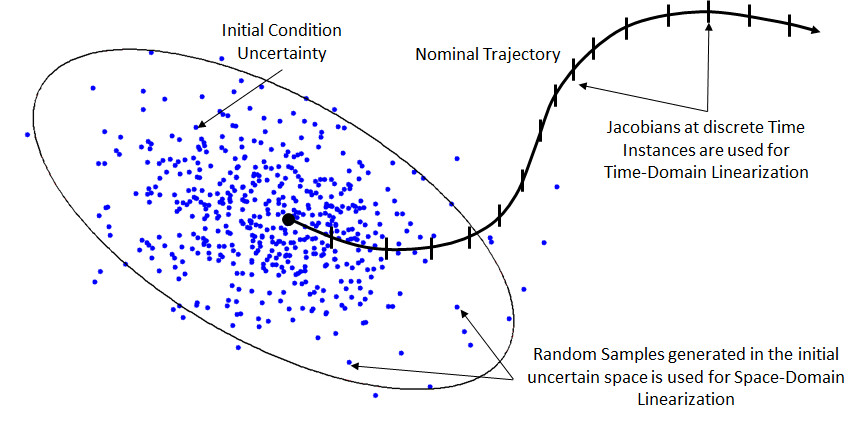
\includegraphics[width=\textwidth]{figures/FIG_3}
\caption{Setup for Time-Domain and Space-Domain Linearization}
\label{fig_lin}
\end{figure}

\subsection{Time-Domain Linearization}
\label{timedomain}

Let us consider the dynamical system given in Equation~\ref{nonlindiffeqn} with the initial condition $\textbf{x}_0$. We consider the nominal trajectory following the definition given in Equation~(\ref{gamma}) as $\gamma_{T,\mu_0}$, where $\mu_0 = E(\textbf{x}_0)$. The \textit{Time-Domain Linearization} considers multiple instances on the nominal trajectory, and the Jacobian of the system at those points. Together, a linear system matrix $A_{t}$ as in Equation~(\ref{lin_syst}) is formulated which uses the trajectory information $\gamma_{T,\mu_0}$ to approximate the actual nonlinear system for the given time interval $[0,T)$. Let us now look at the three methods that can be used for time-domain linearization. 

\underline{\textit{Method I: Average Jacobian:}} In this context, Surana \textit{et al.}~\cite{surana2012iterative} have used the \textit{time-average} of the Jacobian, given by:
\begin{equation}
\bar{J} = \frac{1}{T} \int_{0}^{T} J_t dt
\end{equation}
\noindent where,
\begin{equation}
J_t = \displaystyle \frac{\partial f(\mathbf{x})}{\partial \mathbf{x}} \bigg|_{\phi^t(\mu_0)}
\end{equation}
The weighted adjacency matrix and the graph Laplacian is found out using the definition of $\bar{J}$ instead of the Jacobian at a given point. The \textit{time-average} Jacobian is considered to be the vector field of the overall system with an idea that the Eigenvalues of the graph Laplacian from this system contains the inter-state connection information. 

However, it should be noted that one is ideally interested in the average Eigenvalues and the Eigenvectors of the Jacobian matrix. If the absolute values of the Jacobian are not taken, then one can often get wrong information of the system. Also, Eigenvalues and Eigenvectors of the time averaged Jacobian matrix does not correspond to the average Eigenvalues and Eigenvectors. For example, let us consider a system whose Jacobian at two different time instants are given as: 
\begin{equation}
\begin{array}{l}
A_{k} = \begin{bmatrix}
1.5 & -0.5 \\ -0.5 & 1.5
\end{bmatrix}
\hspace{5mm} A_{k+1} = \begin{bmatrix}
0.8 & 0.5 \\ 0.5 & 2.8
\end{bmatrix} \\
A_{k} + A_{k+1} = \begin{bmatrix}
2.3 & 0 \\ 0 & 4.3
\end{bmatrix}
\end{array}
\end{equation}
Clearly, the adjacency shows coupling effect between the two states at both the time instances, while the Eigenvectors of the matrix $A_k + A_{k+1}$ shows the states to be completely decoupled. Using this idea, the Eigenvalue and Eigenvector information of the adjacency or the Laplacian matrix is carried forward and is used to 
give the map $\psi$. Next, we discuss the two methods of clustering the states space, that do not utilize the \textit{time-averaged} Jacobian. The present methods instead record the inter-state connection information at each instance, carried forward by the Eigenvalues and the Eigenvectors of the Jacobian at each time instance.

\underline{\textit{Method II: Average Graph Laplacian:}} This method calculates the Eigenvalues $\lambda_{t_k}$ and Eigenvector $V_{t_k}$ of the $L_{t_k}$ matrix defined in~(\ref{graphlap}). At each point $\mathbf{x_t}$, the average Eigenvalues and the Eigenvectors are calculated using:
\begin{equation}
\begin{array}{cc}
\bar{\lambda} = \frac{1}{T} \int_{0}^{T} \lambda_t dt & \hspace{5 mm} \bar{V} = \frac{\int_{0}^{T} \lambda_t V_t dt}{\int_{0}^{T} \lambda_t dt} 
\end{array}
\end{equation}
Since, $L_{t_k}$ at any time instance, is a symmetric matrix, the \textit{Average Graph Laplacian} of the approximate linear system for the given time span $[0,T)$ is given as:
\begin{equation}
L^{T_s} = \bar{V} \bar{\lambda} \bar{V}^T
\end{equation}
The number of clusters and the cluster structure are derived using SC and Bayesian NMF.

\underline{\textit{Method III: Average Graph Adjacency:}} In this method, we find out the eigenvalues $\lambda'_{t_k}$ and the eigenvector $V'_{t_k}$ of the matrix $A_{t_k}$ defined in~(\ref{wead}). Next we find the \textit{time-averaged} $\lambda'_{t_k}$ and $V'_{t_k}$ using:
\begin{align}
&\bar{\lambda}' = \frac{1}{T} \int_{0}^{T} \lambda'_t dt 
&\bar{V}' = \frac{1}{T} \int_{0}^{T} V'_t dt  
\end{align}
Since $R_{t_k}$ at each time instant is a symmetric matrix, the \textit{Average Graph Adjacency} of the approximate LTIV system for the given time span $[0,T)$ is given by:
\begin{align}
A^{T_s} = \bar{V}'\bar{\lambda}'\bar{V}'^T
\end{align}

This graph adjacency information $A^{T_s}$ is used to obtain the cluster structure using SC and Bayesian NMF.

\underline{\textit{Averaging out Eigenvector Matrix for Weakly Connected Subsystems:}}
The Jacobian of any WCS in any instance has a block-diagonal matrix-like structure. The position of the bands, however, changes with time as shown in Figure~\ref{Eigenvect}. The pattern although shows discernible blocks, but they are permuted such that averaging over time can lead to erroneous interpretation. Thus, there is a need for proper orientation of the matrix, such that the blocks can be averaged and appropriately identified. An algorithm to correctly orient the Eigenvector matrices in a way that the blocks are easily identified is sketched next. The Algorithm~\ref{alg1} outlines the algorithm to generate a permutation matrix for such transformation of any given matrix $A$.

\begin{algorithm}[H]
\caption{To find out the permutation matrix for matrix $A$}
\label{alg1}
\begin{algorithmic}
\Require Square matrix $A$ 
\Ensure Permutation matrix $P$
\do Initialize $n$ as $size(A)$ \\
\do Initialize the Permutation Matrix $P$ as $abs(A)$ 
\For{$i = 1 \to n$} \\
\do find index $k$ of $max(P(i,:))$ \\
Assign $P(i,:) = 0$ \\
Assign $P(i+1:end,k) = 0$ \\
Assign $P(i,k) = 1$ 
\EndFor 
\end{algorithmic}
\end{algorithm}

\begin{figure}[H]
\centering
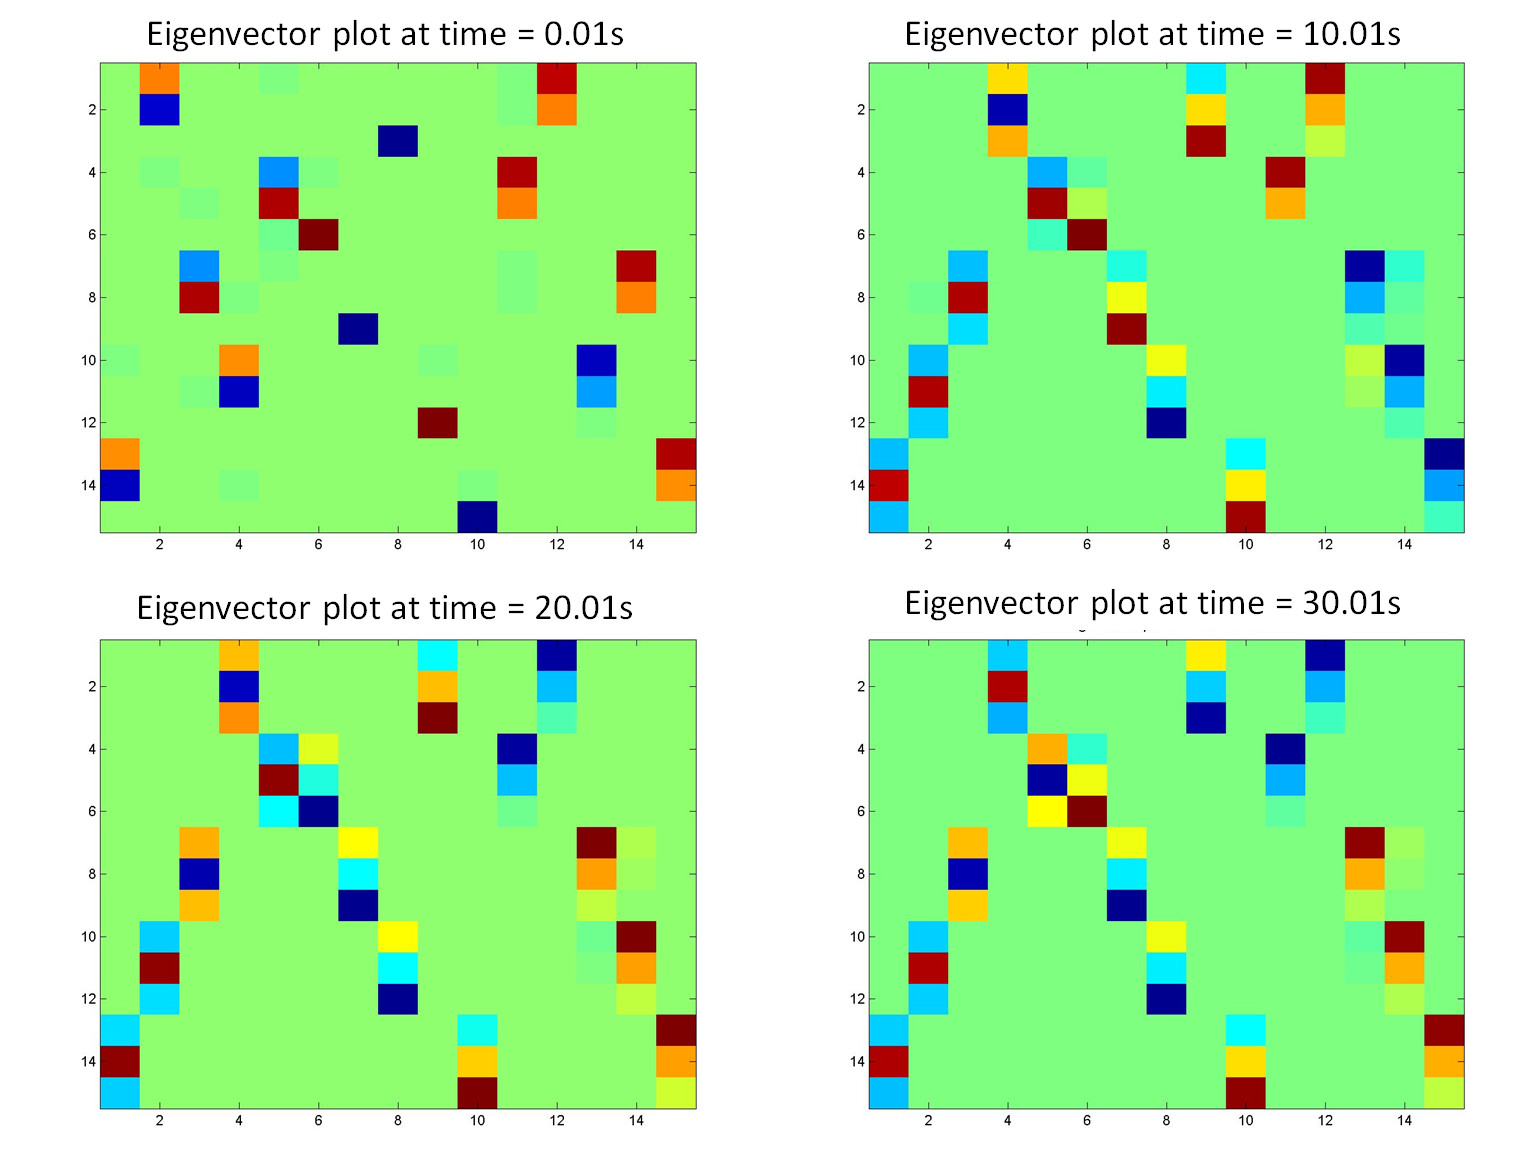
\includegraphics{figures/FIG_4}
\caption{Plot of Eigenvector Matrix of $W_t$ for a WCS at different time instance}
\label{Eigenvect}
\end{figure}

The motivation of the algorithm is to estimate a permutation matrix $P$, so that when it is multiplied with the Eigenvector matrix $W_t$, the resultant matrix has a block-diagonal structure. The algorithm begins with $P$ being initialized to $abs(A)$. Then, in each row of $P$, the element with the maximum value is identified. The component of the cell with the maximum value is assigned to 1 while the rest of the elements in the corresponding row and column are assigned to 0. By adopting this technique, one is guaranteed to obtain the permutation matrix that will give a block diagonal matrix when multiplied with the Eigenvector matrix. 

\begin{figure}[H]
\centering
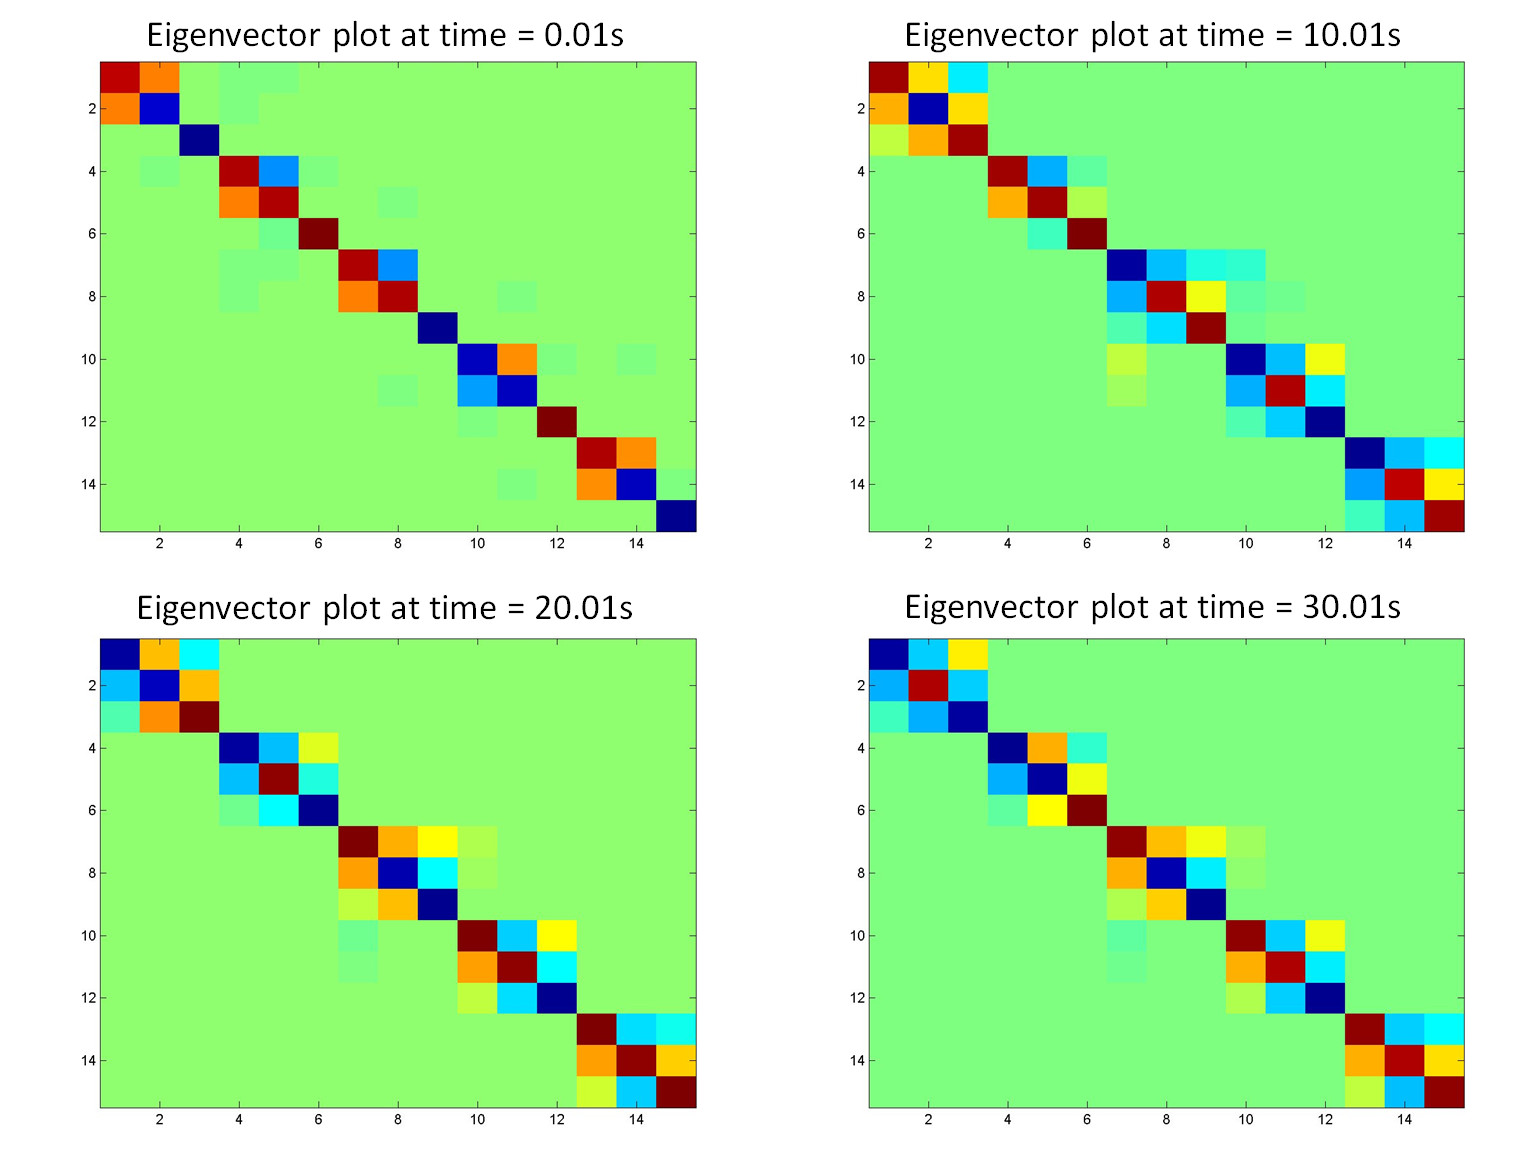
\includegraphics{figures/FIG_5}
\caption{Organized plot of Eigenvector Matrix of $W_t$ for a WCS at different time instance}
\label{Eigenvect2}
\end{figure}

The matrix $P$, once generated, can be used to determine the block matrix using $A_2 = A P^{-1}$. The given algorithm is valid only for decoupled or very weakly coupled oscillators. With increasing coupling strength, the Eigenvectors corresponding to the coupling function gets priority over the states, resulting in an improper result. The corresponding $A_2$ matrices for the Eigenvector matrices given in Figure~\ref{Eigenvect} are given in Figure~\ref{Eigenvect2}. Figure~\ref{Eigenvect2} shows the Eigenvector matrices when operated under the obtained permutation matrix. The figures indicate clear block-diagonal structures. This orientation facilitates easy averaging of the Eigenvector matrices. The corresponding positions of the Eigenvalues are also noted using the same permutation matrix. Thus, both the Eigenvector and the Eigenvalue information follows a continuous pattern throughout the time interval and their average lead to an interpretable information for the application of the clustering algorithm. Note that the block-diagonal structure shows more than the anticipated number of clusters at time t = 0, and then, the diagonal structure evolves with time. This behavior is nicely captured when the matrix is averaged out over time. 

\subsection{Space-Domain Linearization and Ergodicity}
\label{stat_lin_section}

In this section, the space-domain linearization method which, unlike the \textit{Time-Domain Linearization} techniques uses the initial condition uncertainty $\textbf{x}_0$, and not the nominal trajectory $\gamma_{T,\mu_0}$ is described.
Let us revisit the Taylor series expansion given in Equation~(\ref{taylor}). Given nonlinear function $f(\textbf{x})$ about a given point $\mu_t$ we obtain,
\begin{equation}
\label{jacobian}
f(\textbf{x}) = f(\mu_t) + Df(\mu_t) (\textbf{x} - \mu_t) + \mathcal{O} ||(\mathbf{x}  - \mu_t)^T(\mathbf{x}  - \mu_t)||
\end{equation}   
where, $\mu_t = E(\textbf{x}_t)$ and $Df(\mu_t)$ is the Jacobian of $f(\cdot)$ about $\mu_t$. Thus, the estimates of the linear model as in Equation~(\ref{linsyst}) are  computed as,
\begin{equation}
A_j = Df(\mu_t) \hspace{5 mm} b_j = f(\mu_t)
\end{equation}
The error due to such approximation is defined as,
\begin{equation}
\epsilon = f(\textbf{x}) - f(\mu_t) - Df(\mu_t) (\textbf{x} - \mu_t)
\end{equation} 
Hence, due to linearity of the operator $E(\cdot)$, the error can be calculated as $E \left[f(\textbf{x})\right] - f(\mu_t)$. The computed error can increase if $f$ is a highly nonlinear function. Topologically speaking, for all realization of $X(t,\omega) = w$, the trajectory $\phi^t(w)$ will be solved along the direction given by $Df(\mu_t)$ and not in the direction along $Df(w)$.
Other forms of linearization have been used in the past to simplify a nonlinear model. For example perturbation-based model~\cite{de2012efficient}, or Jacobian-based model~\cite{carbonell2007numerical,he2011enhanced,guardone2002roe} or more accurate approximation of nonlinear system~\cite{steeb1980non} linearizes the nonlinear system about a single point only. Therefore such existing methods suffer the same setback as described above. Also, while gradient-based methods need the knowledge of the exact Jacobian of the system, perturbation based method are highly sensitive to the amount of perturbation used. 

\underline{Statistical Linearization}: Spanos~\cite{roberts1986stochastic} suggested the technique of statistical linearization, by which a given nonlinear function $\textbf{x}_t$ of the random variable $\textbf{x}$ defined over $(\Omega,\mathcal{F},P_{\textbf{x}})$ can be approximated by a linear expression $\textbf{x}$. The approximate linearization of the function $f(\cdot)$ is given as,
\begin{equation}
\label{lin_model}
f(\textbf{x}_t) = b_{sl} + A_{sl}(\textbf{x}_t - \mu_t)
\end{equation}
Where,
\begin{equation}
\min_{A,b} J =  \int_{\Omega_t} ||f(z_t) - A_{sl}(z_t - \mu_t) - b_{sl} ||_2 p_{\textbf{x}_t} (z) dz 
\end{equation}
The system is much more accurate and has an expression of the exact solution and does not require the exact expression for the nonlinear velocity function and its Jacobian. The estimates of this model is given by the stationary solutions to the optimization problem, given as,
\begin{equation}
\label{stat_lin}
\begin{array}{rl}
\displaystyle \frac{\partial J}{\partial A_{sl}} = 0  & \Rightarrow  A_{sl} \; E[(\textbf{x}_t - \mu_t)^T (\textbf{x}_t - \mu_t)] - E[f(\textbf{x}_t - \mu_t)^T] = 0\\
& \Rightarrow A_{sl} = E[f(\textbf{x}_t - \mu_t)^T] P_{\textbf{x}_t \textbf{x}_t}^{-1} \\
\displaystyle \frac{\partial J}{\partial b_{sl}} = 0  & \Rightarrow b_{sl} - E[f] = 0\\
& \Rightarrow b_{sl} = E[f] 
\end{array}
\end{equation}

Such a linearization is \textit{Jacobian-free} and incorporates the information of the whole probability space, rather than just the mean of it. Figure~\ref{compare2} shows the difference in linearized matrix formulated by both Jacobian and Statistical Linearization from two different orientation of the $xyz$ axes. The schematic represents the approximation difference between the matrix formulated by either of the linearization technique and the Jacobian of the actual system about random samples generated in a given 2-D probability space. The $xy$ coordinates represent the state variables, while the $z$ axis shows the metric $||J_x - A||_2$, $x$ being a random sample. Figure~\ref{compare} shows the schematic difference in the behavior of the propagation of the linearized model against the actual nonlinear propagation. Since, the direction of trajectory for all points $\mathcal{X} \in \Omega$ can be very different from the trajectory for $\mathcal{X} = \mu_t$, the expected error in propagation for the Jacobian-based Linearized model can be very high. On the contrary, the Statistical Linearization minimizes this error. Hence, the trajectories for all $\mathcal{X} \in \Omega$ is expected to be approximated much better by the propagation $\dot{\textbf{x}}_t = A_{sl} \textbf{x}_t + b_{sl}$.

\begin{figure}[H]
        \centering
        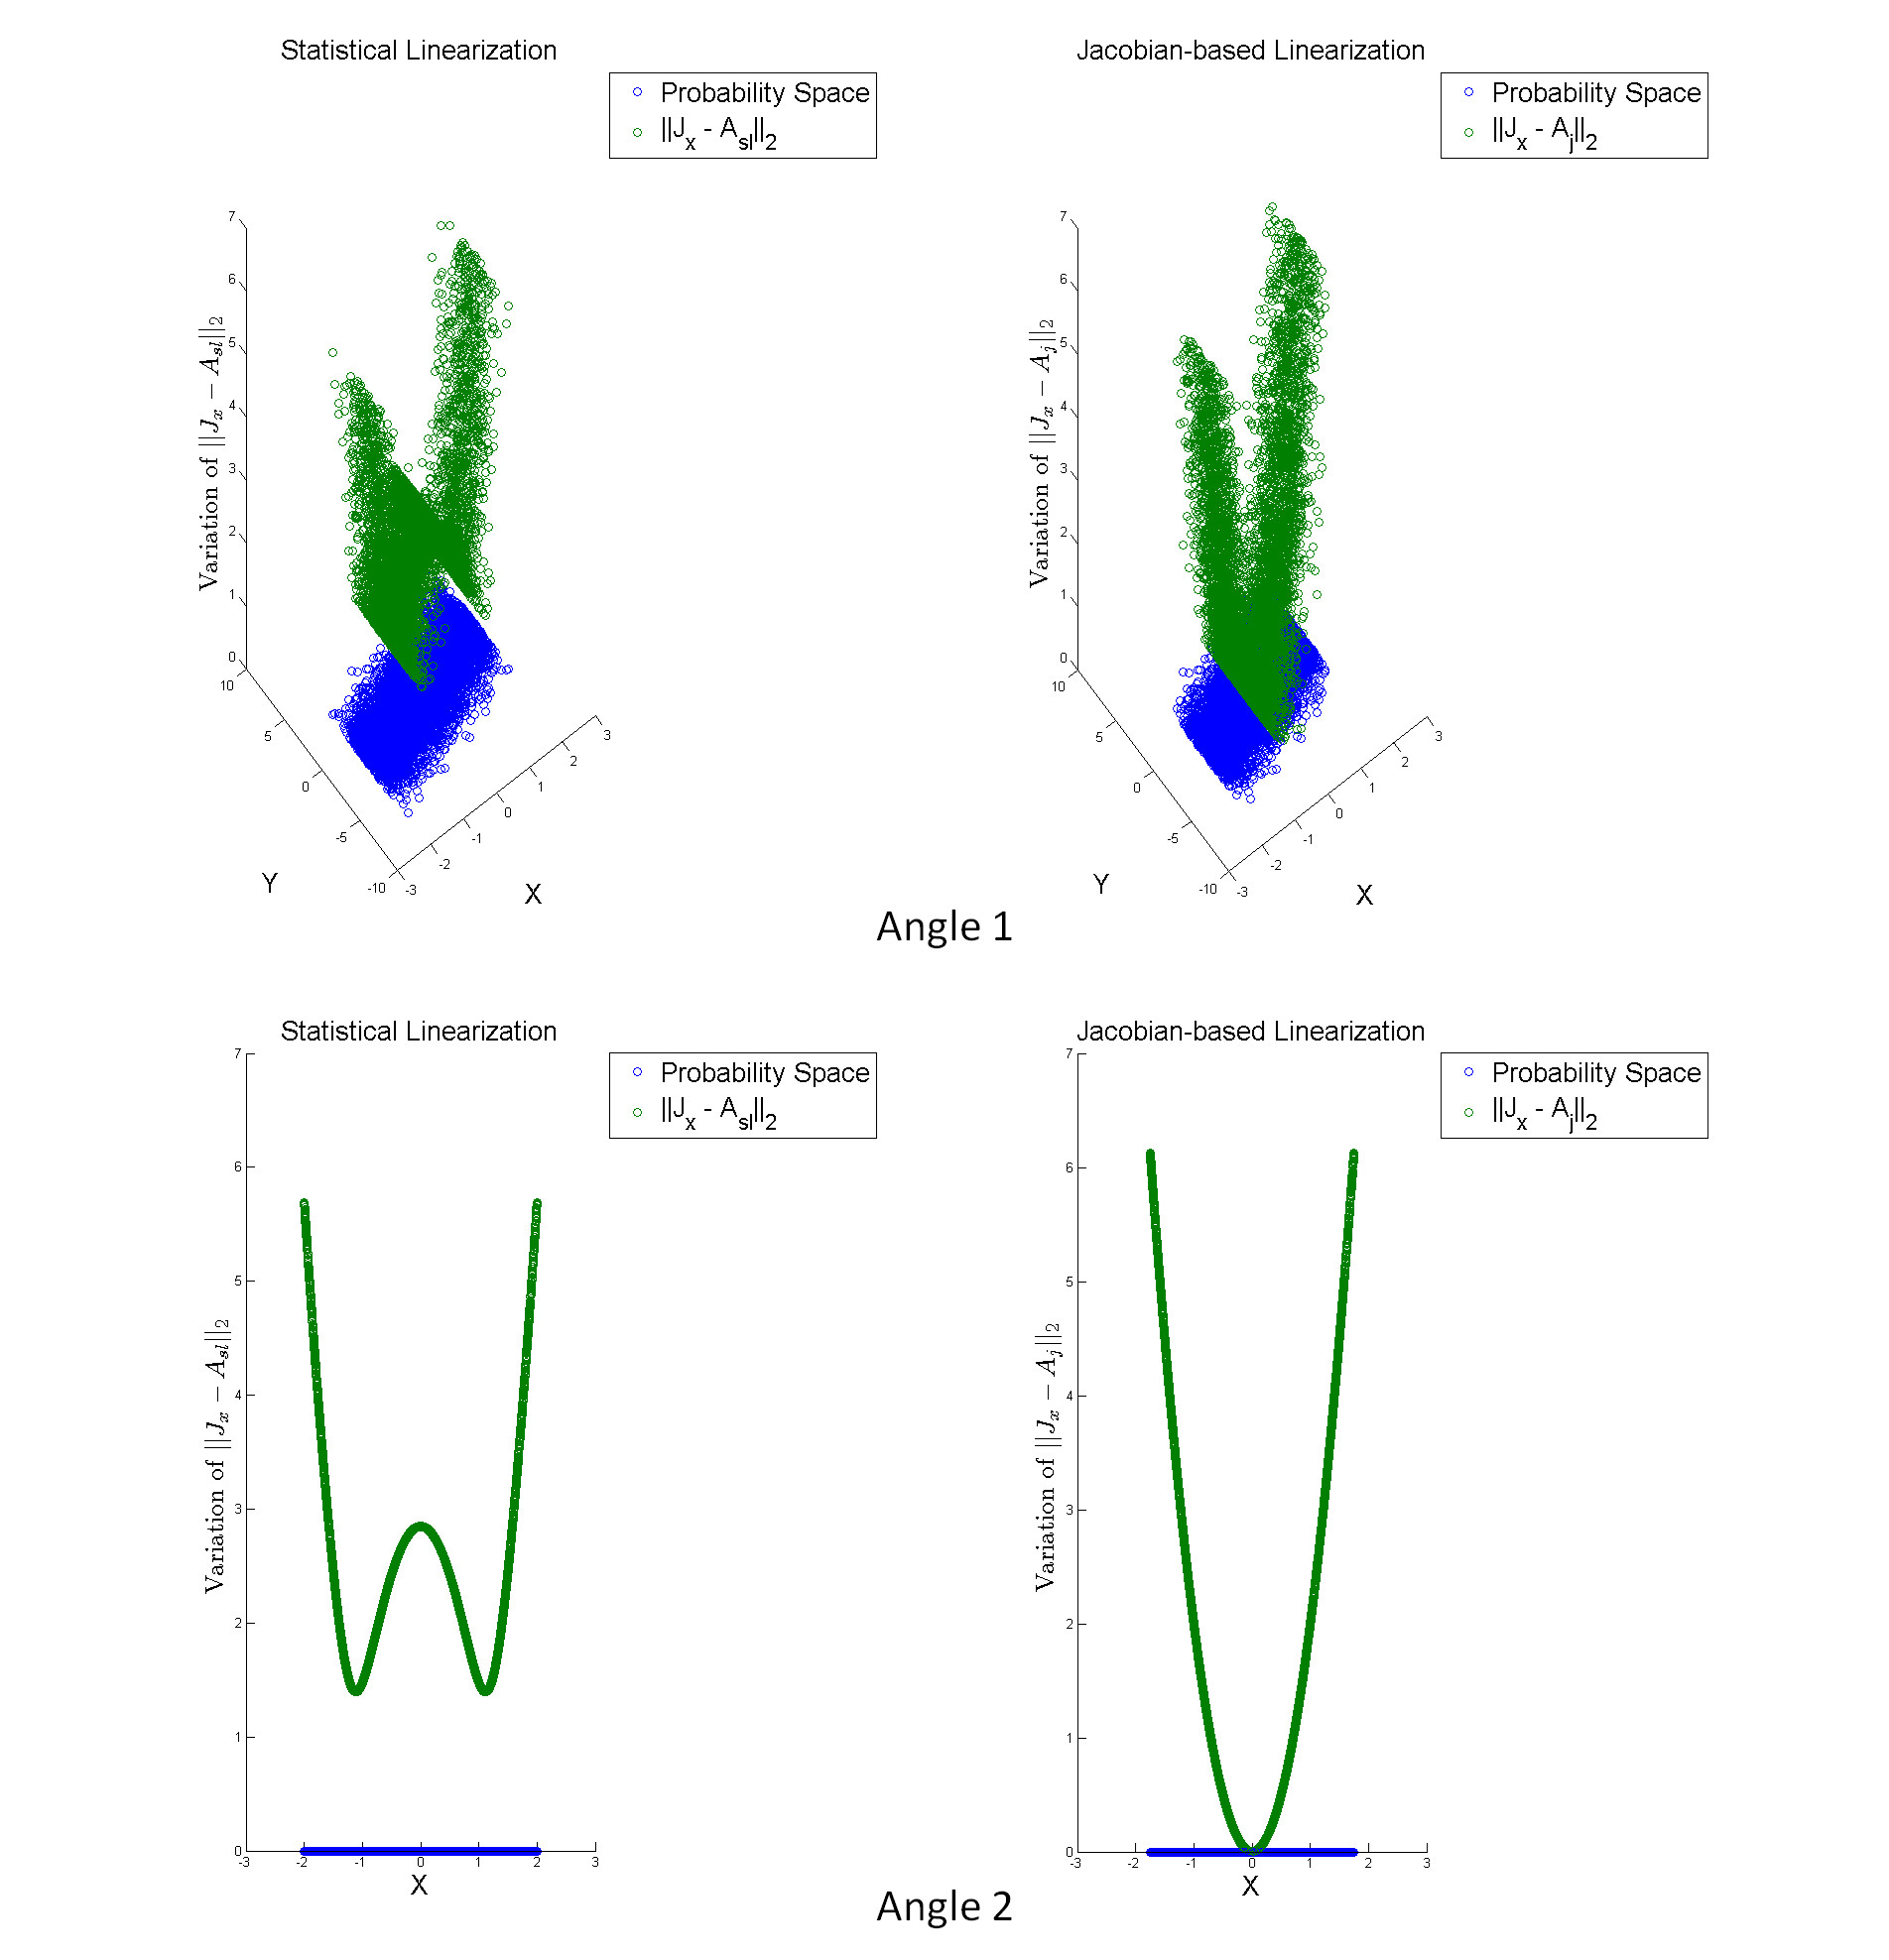
\includegraphics{figures/FIG_6}
        \caption{Comparison between Jacobian-based linearization matrix and Statistical linearization matrix}
        \label{compare2}
\end{figure}


\begin{figure}[H]
        \centering
        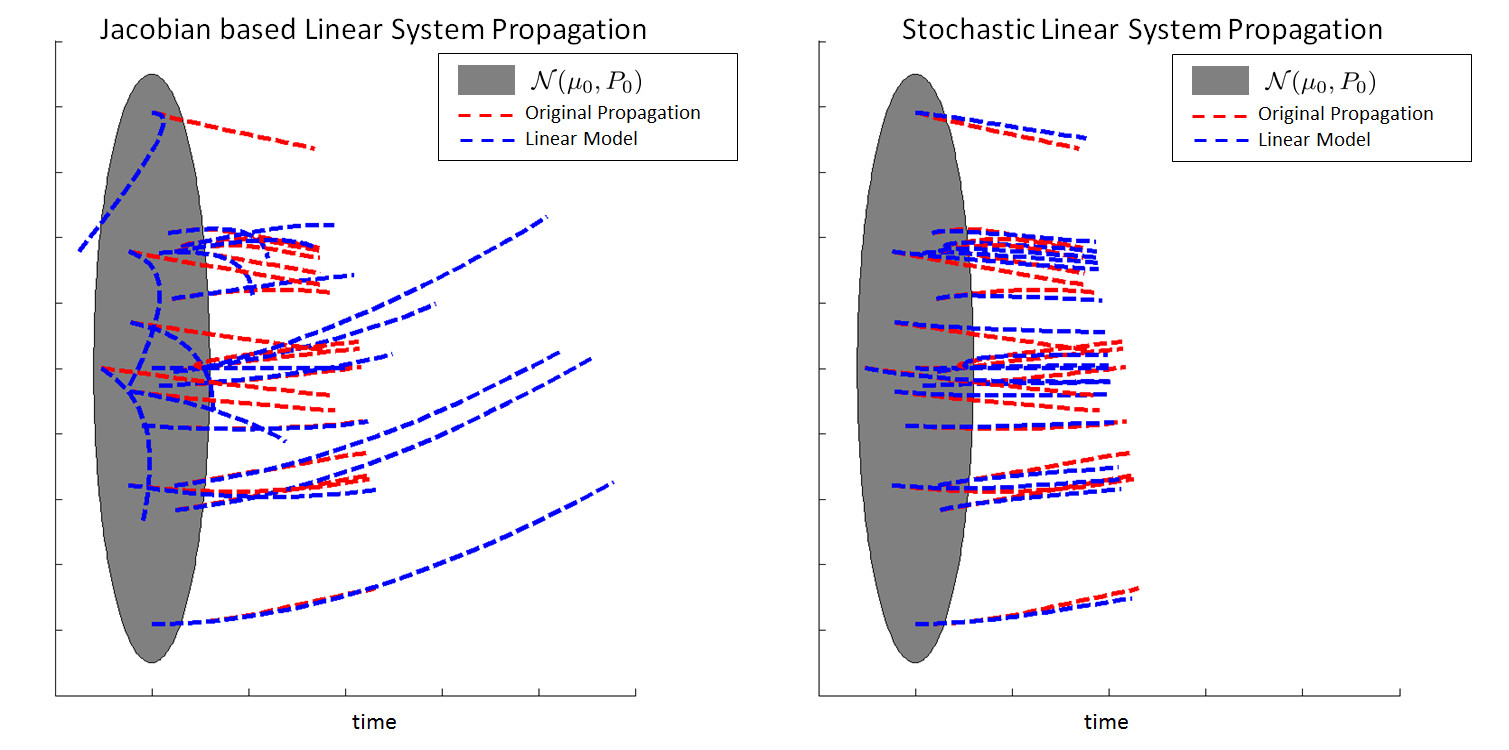
\includegraphics{figures/FIG_7}
        \caption{Comparison between propagation of Jacobian-based linearization and Statistical linearization}
        \label{compare}
\end{figure}

Let us now consider a nonlinear system defined by the equation $\dot{\textbf{x}}_t = f(\textbf{x}_t)$, with $\textbf{x}_t \sim \mathcal{N}(\mu_t,\sigma^2 I)$, $\textbf{x}_t \in \mathbb{R}^n$. The sigma points $\mathcal{X}$, the matrix $\mathcal{X} -\mu_t$ for $\textbf{x}_t$ and the corresponding weight vector will be given by the Equation~(\ref{sigmapt}) as,
\begin{equation}
\begin{array}{lcr}
\mathcal{X} = \begin{bmatrix}
\mu_t \\
\mu_t + \sigma  \lambda I_{n \times n} \\
\mu_t - \sigma \lambda I_{n \times n}
\end{bmatrix} &
\mathcal{X} - \mu_t =  \begin{bmatrix}
\textbf{0}_{1 \times n} \\
\sigma \lambda I_{n \times n} \\
- \sigma \lambda I_{n \times n}
\end{bmatrix}  &
 W = \begin{bmatrix}
\frac{\kappa}{\lambda^2}, \frac{1}{2\lambda^2}, \frac{1}{2\lambda^2}, \ldots , \frac{1}{2\lambda^2}
\end{bmatrix}^T_{1 \times (2n + 1)}
\end{array}
\end{equation} 
\noindent where, $\lambda = \sqrt{n+ \kappa}$. Any element $A_{{sl}_{ij}}$ of the Statistical Linearization matrix is thus given by the Equation~(\ref{stat_lin}) as,

\begin{equation}
\begin{array}{rl}
A_{{sl}_{ij}} = & \frac{1}{\sigma^2} \bigl[f_i(\mu_t)\cdot 0 \cdot W(0) + f_i(x_1 + \sigma \lambda,x_2,\ldots,x_n)\cdot 0 \cdot W(1) + \ldots \\
& + f_i(x_1 ,\ldots,x_j + \sigma \lambda,\ldots, x_n)\cdot \sigma \lambda \cdot W(j-1) \bigr.\\
& \left. + \ldots + f_i(x_1 ,\ldots,x_j - \sigma \lambda,\ldots, x_n) \cdot - \sigma \lambda \cdot W(j + n) \right] \\
= & \frac{f_i(x_1 ,\ldots,x_j + \sigma \lambda,\ldots, x_n) - f_i(x_1 ,\ldots,x_j - \sigma \lambda,\ldots, x_n)}{2 \sigma \lambda}
\end{array}
\end{equation}
\noindent With $\sigma \lambda \rightarrow 0$, the above expression of $A_{{sl}_{ij}}$ approaches the analytic expression for the derivative $\frac{\partial f_i}{\partial x_j}$. Hence, the Statistically linearized matrix $A_{sl}$ approximates the expression for the Jacobian $Df(\mu_t)$ for very low covariance values. 
 The Statistical Linearization is the only linearization technique among the rest, which can capture the contribution of both the vector field and the covariance information towards the coupling between the state variables. With high covariance values, the variation in $A_{sl}$ also increases. This behavior is not captured by any of the time-domain linearization methods. The method of Statistical Linearization will be referred to as SL in subsequent sections. 
 
Now, let us consider the initial probability space $(\Omega,\mathcal{F},P_{\textbf{x}_0})$ such that, $\phi:\Omega \rightarrow \Omega$ is a measure-preserving transformation. Since, $f$ is already a real-valued measurable function, hence by Birkhoff's Ergodic Theorem~\cite{Katok1995}, 

\begin{equation}
\lim_{n \rightarrow \infty} \frac{1}{n} \sum_{k=0}^{n-1} f \left( \phi^k (x) \right) = \int_{\Omega} f dP_{\textbf{x}_0}, \hspace{5 mm} x \in \Omega \text{ almost everywhere}
\end{equation}

\noindent which implies, that the space-domain average equals the time-domain average of the function $f$ for the nominal trajectory. Now, the above linearization techniques give us the formulation for the time average linearization $A_t$ and the state-space linearization $A_{sl}$. Thus, by property of ergodicity, we assume both the linearization to be equal. 

As discussed, the nonlinear system needs to be converted into a time-invariant linear model, where one can use the linear system matrix as a graph adjacency matrix.

\section{Non-overlapping Graph Clustering Methods}
\label{non_overlap_clustering}

The preliminary concept of clustering dates back to 1939~\cite{tryon1939cluster}. Clustering techniques and their comparisons are abundant. Domains like gene-clustering~\cite{eisen1998cluster,sturn2002genesis}, pattern recognition~\cite{bishop2006pattern,baraldi1999survey}, social media~\cite{lancichinetti2008benchmark}, image segmentation find abundant usage of data clustering techniques. Early reviews~\cite{cormack1971review,everitt1972cluster} mainly focused on heterogeneous datasets in which the affinity between the data points could be used to create groups of \textit{similar} and \textit{unlabeled} data objects. The research in clustering domain also focuses on measures to define the affinity, such that the number of groups of similar objects or \textit{clusters} can be increased. Researchers also have focused on the comparative study of different clustering algorithms such as hierarchical clustering, k-means clustering, Minimal Spanning Tree, and Fuzzy clustering~\cite{jain1988algorithms,jain1999data}. These reviews mainly focused on image segmentation and pattern recognition domains. The problems in these domains deal with a static dataset. Although the methods mentioned above are widely used even today on large datasets, these methods cannot be directly applied to our area of interest. The inapplicability of these existing clustering methods directly to the problem of WCS identification comes from the fact that such problem involves dynamics of the overall system. In dynamic system setting, the dataset is not static. 

For dynamic systems, one way to implement any clustering technique is to apply the clustering to the data at every time step. Another way to use a clustering technique to identify WCSs is to optimize the cluster structure in a way such that the error accumulated over the time is minimized. Both methodologies can be adopted only on a small dataset and for a short time. The curse of dimensionality in nonlinear systems is also tackled by finding a reduced order model~\cite{calinski1974dendrite,matthies2003nonlinear,wang2011two,carlberg2013gnat}. However, these methods are not useful in finding WCSs in large-scale systems. Kaneko~\cite{kaneko1990clustering,kaneko1990globally} studied clustering in a coupled nonlinear system. Kaneko studied coupled nonlinear models in the discrete-time scenario. The methods of detecting clusters are easy to implement. However, the applicability is limited to the specific type of problem discussed. Additionally, the presented methods cannot be used to study continuous time dynamic systems. The existence of cluster structure in coupled non-identical clusters has been reviewed by Lu \textit{et al.}~\cite{lu2010cluster}. They have shown that individual clusters under diffusive coupling can get fully synchronized if the coupling strength is high. The concept of Laplacian and Spectral Clustering has been introduced in this context~\cite{dellnitz2003congestion, varigonda2004graph}, and later has been studied for UQ in nonlinear dynamics~\cite{xia2011clustering,surana2012iterative, sorrentino2015complete}. 

Consider a linear system given by:
\begin{equation}
\label{lindiffeqn}
\dot{\mathbf{x}}_t = A \mathbf{x}_t + b
\end{equation}
The set of state variables $\textbf{x} \in \mathbb{R}^N$ are treated as vertices of a $N$-order undirected graph.  The association between each vertex is defined by the probability of transition between each state. At the end of the clustering, the subsets or the random vectors $\mathbf{y}_j$s are obtained. 
Such a system is easy to partition since the states are in a linear combination of each other. Standard methods such as PCA, POD, Factor Analysis, Jordan block decomposition and others. can be used to decompose the overall system. However, such methods either aim at finding a subspace of lower dimension or decouple the system using canonical coordinates. In the current work, our aim is slightly different and is focused on finding weakly or strongly connected subsystems, whose ensemble explains the dynamics of the overall large system.  

Let us consider a \textit{weakly coupled linear} system characterized by the matrix $A$. Decomposition of such a connected graph is based on the theory formulated by Fiddler~\cite{fiedler1973algebraic,fiedler1975property}, by which connectivity information is stored in the Eigenvalues and Eigenvectors of the adjacency matrix of a graph. The adjacency matrix can be written as~\cite{varigonda2004graph},
\begin{equation}
\label{adjcncy}
W = 0.5(P + P^T)
\end{equation}
where, $P$ is defined as,
\begin{equation}
\label{probmat}
p_{i,j} = | A_{ij} | /  \sum_{j=1}^n | A_{ij} |
\end{equation}
This transformation yields a matrix that stores the adjacency information of a weighted undirected connected graph. The transformation can also be interpreted from a probabilistic point of view. The matrix $A$ evidently stores information about the transition between state variables. This matrix $P$ is a (right) stochastic matrix as $p_{i,j} \ge 0$ for all $i,j$ and $\sum_j p_{i,j} = 1$ \cite{wolfowitz1963products}. Once, the $P$ matrix is obtained, the unique \textbf{stationary distribution} of $P$ (say $\pi_i$) or the left Eigenvector corresponding to the Eigenvalue of magnitude 1 is calculated. The stationary distribution is defined as, 
\begin{equation}
\pi_{j} =  \sum_{i \in S} \pi_i p_{ij} 
\end{equation}
Varigonda \textit{et al.}~\cite{varigonda2004graph} have used the following matrix definition as a graph adjacency matrix,
\begin{equation}
\label{wead}
W = MR = \frac{1}{2}(MP + (MP)^T)  \hspace{5 mm} M = diag(\pi_1,\pi_2,\ldots,\pi_n)
\end{equation}
where, the matrix $R$ is a reversible stochastic matrix given as~\cite{dellnitz2003congestion}: 
\begin{equation}
\label{revprobmat}
R = \frac{1}{2}(P + M^{-1} P^T M)
\end{equation}
A stationary Markov chain is said to be reversible if the transition matrix $R$ and the stationary distribution $\pi$ satisfies the following relation
\begin{equation}
\pi_i R_{ij} = \pi_j R_{ji}
\end{equation}
Under this transformation given in Equation~(\ref{revprobmat}), 
\begin{equation*}
\begin{array}{rl}
R_{ij} &= \frac{1}{2}\left(p_{ij} + \frac{1}{\pi_i}p_{ji}\pi_j \right) \\
\sum_j R_{ij} &= \sum_j \frac{1}{2}\left(p_{ij} + \frac{1}{\pi_i}p_{ji}\pi_j \right) \\
&= \frac{1}{2} + \frac{1}{2 \pi_i} \sum_j p_{ji} \pi_j = \frac{1}{2} + \frac{1}{2} =1
\end{array}
\end{equation*}
The following shows that $\pi_i'$s are also stationary transition probability distribution for $R$:
\begin{equation*}
\sum_i \pi_i R_{ij} = \frac{1}{2}\left[ \sum_i p_{ij} \pi_i + \pi_j \sum_i \pi_i \frac{1}{\pi_i} p_{ij} \right] = \frac{1}{2} \left(\pi_j + \pi_j  \right) = \pi_j
\end{equation*}
Thus, the adjacency matrix given by Equation~(\ref{adjcncy}) can be considered to be equivalent to a reversible matrix. Next, details related to several methods of graph clustering and their behaviors is outlined.


\subsection{Spectral Clustering}

Spectral Clustering (SC)~\cite{von2007tutorial} is a method of clustering a given graph using the spectrum or the Eigenvalue information. It uses a symmetric weighted adjacency matrix for clustering and obtains the Laplacian information from the given adjacency matrix. Given the adjacency matrix defined in Equation~\ref{wead}, the matrix can be decomposed into a set of well-connected components. By Matrix-Tree theorem~\cite{merris1994laplacian} $Rank(L) = n - w(G)$, whereby $L$ is the Laplacian of a binary adjacency matrix, $n$ is the order of matrix $A$, and $w(G)$ is the number of connected components. 
Graph Laplacian~\cite{merris1994laplacian,mohar1991laplacian} of $A$ is defined as:
\begin{equation}
L = D - W
\end{equation}
Where, $D$ is the degree matrix~\cite{bollobas1982graph}, and $W$ is the weighted adjacency matrix defined as in Equation~(\ref{wead}). Clearly, this matrix is both symmetric and positive semi-definite and one can trivially see that the lowest Eigenvalue is 0. For a weighted graph, the symmetric Graph Laplacian~\cite{chung1997spectral} is taken as:
\begin{equation}
\label{graphlap}
L = I - D^{-1/2} W D^{-1/2}
\end{equation}
The above formulation results from the minimization of the normalized cut objective function for clustering a given weighted adjacency graph~\cite{shi2000normalized}. Besides, the transformation serves the purpose of scaling down the matrix by its adjacency, which makes the analysis to be much easier. The properties of symmetry and positive semi-definite remains intact, and additionally it has other properties such as:
\begin{itemize}
\item $0 \leq \lambda_i \leq \sqrt{2}$
\item $\sum_i \lambda_i \leq n$, with the equality holds when there is no isolated vertex. 
\item $\lambda_1 =0, \lambda_{n-1} \geq \frac{n}{n-1} $
\end{itemize} 

Figure~\ref{fig:spectral} shows a schematic of the SC methodology. Given an adjacency matrix (Figure~\ref{fig:sc_adjacency}), one computes the eigenvalue of the normalized graph Laplacian as in Equation~\ref{graphlap} (Figure~\ref{fig:sc_eigen}). From the eigenvalue plot, one decides the cluster structure from the eigenvector matrix corresponding to number of zero eigenvalues (Figure~\ref{fig:sc_cluster}).

\begin{figure}[H]
\centering
\begin{subfigure}{0.32\textwidth}
\centering
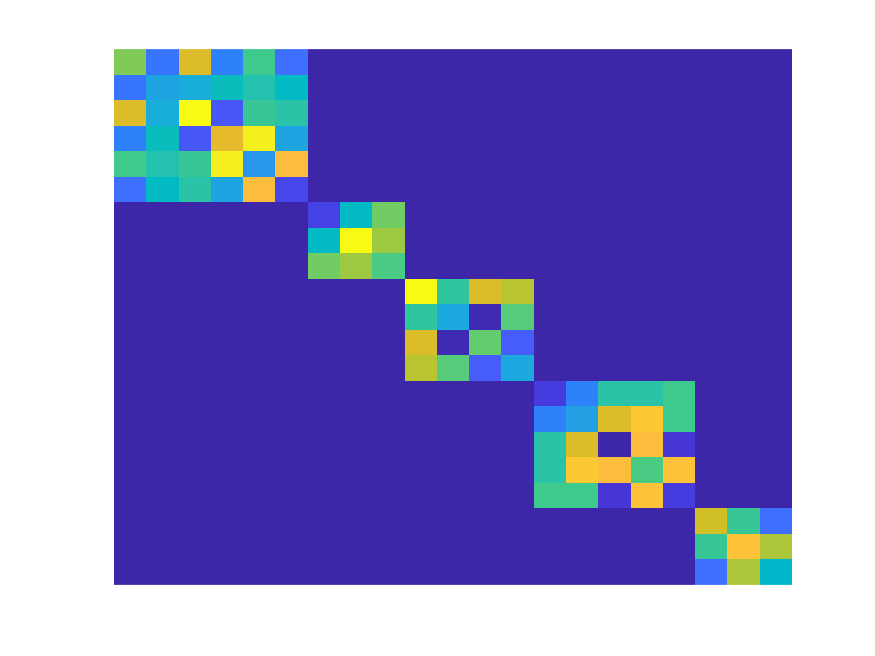
\includegraphics[width=\textwidth]{figures/adjacency}
\caption{}
\label{fig:sc_adjacency}
\end{subfigure}
\begin{subfigure}{0.32\textwidth}
\centering
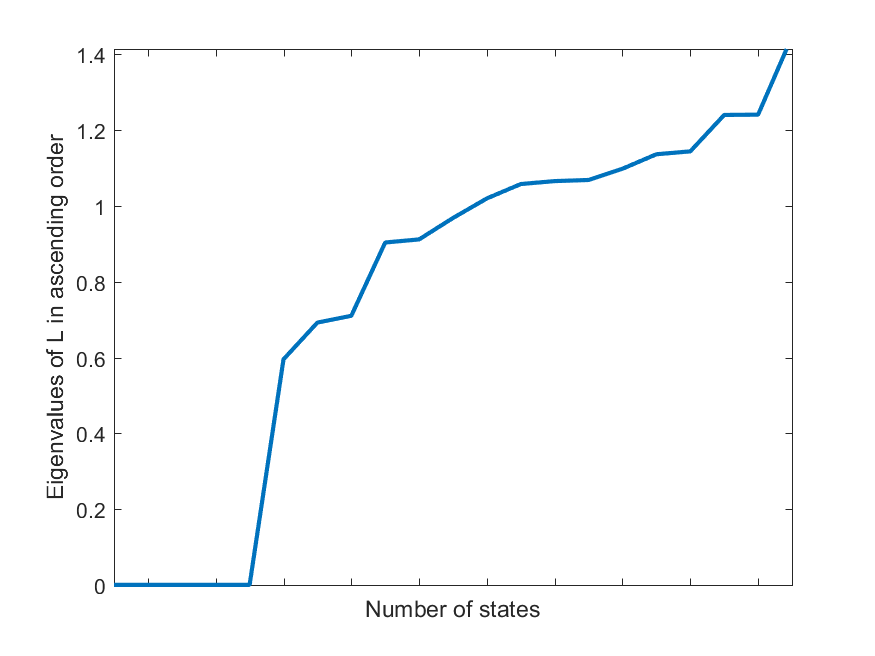
\includegraphics[width=\textwidth]{figures/eig}
\caption{}
\label{fig:sc_eigen}
\end{subfigure}
\begin{subfigure}{0.32\textwidth}
\centering
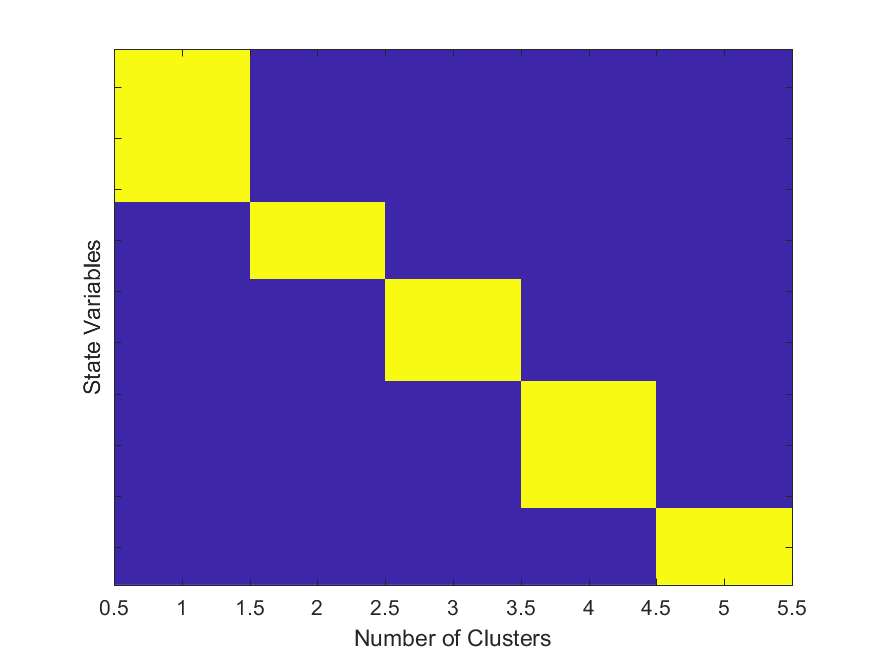
\includegraphics[width=\textwidth]{figures/cluster}
\caption{}
\label{fig:sc_cluster}
\end{subfigure}
\caption{Schematic of Spectral Clustering: (a) shows a typical adjacency matrix comprising of discernible blocks (b) shows the eigenvalue plot of the symmetric normalized Laplacian for the corresponding adjacency and (c) shows the cluster structure derived from the eigenvector of the corresponding zero eigenvalues}
\label{fig:spectral}
\end{figure}



This method is essentially used to identify clusters in a Block-Diagonal Matrix of the form 
\begin{equation}
\label{block}
A = \bigoplus_{i=1}^m A_i = \begin{bmatrix}
A_1 & 0 & \ldots & 0 \\ 0 & A_2  & \ldots & 0 \\ \vdots & \vdots & \ddots & \vdots \\  0 & 0 & \ldots & A_m
\end{bmatrix}
\end{equation}
For a fully connected graph $A_j$, the corresponding stochastic matrix $P_j$ will have exactly one Eigenvalue with magnitude 1, and the symmetric graph Laplacian $L_j$ will have exactly one Eigenvalue of magnitude 0. The graph Laplacian of a block-diagonal adjacent matrix also takes the form of a block diagonal matrix as,
\begin{equation*}
L_{sym} = \bigoplus_{i=1}^m L_i = \begin{bmatrix}
L_1 & 0 & \ldots & 0 \\ 0 & L_2  & \ldots & 0 \\ \vdots & \vdots & \ddots & \vdots \\  0 & 0 & \ldots & L_m
\end{bmatrix}
\end{equation*}
The Eigenvalue plot for the Laplacian gives us the number of clusters, which is approximately equal to Number of \textbf{almost zero} Eigenvalues. Sometimes an Eigenvalue plot becomes too ambiguous in terms of finding the correct point that refers to the highest \textit{almost zero} value. Even a naked eye judgment fails to take such decision. Hence a `knee point' algorithm has been adopted~\cite{salvador2004determining}, that finds out the point of maximum curvature of the Eigenvalue plot, by estimating a pair of straight lines that best describes the plot. 


\subsection{Non-negative Matrix Factorization}

Non-negative Matrix Factorization (NMF) (earlier formulated as Positive Matrix Factorization~\cite{paatero1994positive}) belongs to the class of problem, whereby a given matrix $A \in \mathbb{R}^{n \times m}_+$ is factorized as
\begin{align}
W = XY
\end{align}  
Where, the resultant factor matrices are $X \in \mathbb{R}^{n \times p}_+$ and $Y \in \mathbb{R}^{p \times m}_+$, and $P$ is the right stochastic matrix defined in Equation~(\ref{probmat}). The factorization can be done in such a way such that, $p \ll n $ and $p \ll m$. Pioneering research in this field has been conducted by Lee and Seung~\cite{lee1999learning}. They have solved a simple least square formulation to get the update equations for $X$ and $Y$. 

Since then, NMF has been a subject of immense interest and have been found to be very useful in Graph Clustering, Data storage, and Community Detection.
Ding \textit{et al.} have shown that the symmetric NMF (i.e., where $W$ is symmetric, and $X = Y$) is similar to kernel k-means and Spectral Clustering~\cite{ding2005equivalence}. Wang \textit{et al.}~\cite{wang2011community} have used the symmetric NMF to detect community in an interconnecting network. Wang \textit{et al.} have formulated a problem of factorizing a symmetric graph adjacency matrix as,
\begin{align}
\min_{\hat{X} \geq 0}  \bigg| \bigg| W - \hat{X}\hat{X}^T \bigg| \bigg|_{F}^2
\end{align}
where, the resultant factor matrix $\hat{X}$, is normalized. After normalization, each element corresponds to the probability of occurrence of an element in the community. A  Probabilistic approach to NMF has been adopted by Zass and Shashua~\cite{zass2005unifying}. Bayesian framework has been adopted by Virtamen \textit{et al.}~\cite{virtanen2008bayesian} and later by Schmidt \textit{et al.}~\cite{schmidt2009bayesian} and are shown to be better performing than existing algorithms. However, a key question about the ideal value of $p$ to enable the clustering, has been addressed experimentally. Psorakis \textit{et al.}~\cite{psorakis2011overlapping} have proposed a Probabilistic Graphical framework, to capture the probability of the existence of a particular element in a community and to iteratively decide the smallest possible value of $p$, such that the error $\min_{\hat{X} \geq 0}  \bigg| \bigg| W - \hat{X}\hat{X}^T \bigg| \bigg|_{F}^2$ is minimized. The Bayesian NMF uses a probabilistic graphical model given in Figure~\ref{bnmf}.  

\begin{figure}[H]
\centering
\tikzstyle{block} = [circle, draw, fill=blue!20, 
    minimum size=.5cm, text centered, minimum height=4em]
\tikzstyle{line} = [draw, -latex']
\begin{tikzpicture}
\node [block] (A) {$\beta_k$};
\node [block, left of=A,yshift=-2cm,xshift=-1.5cm] (B) {$a$};
\node [block, left of=A,yshift=2cm,xshift=-1.5cm] (C) {$b$};
\node [block, right of=A,yshift=2cm,xshift=1.5cm](D){$X_{ik}$};
\node [block, right of=A,yshift=-2cm,xshift=1.5cm](E){$Y_{kj}$};
\node [block, right of=D,yshift=-2cm,,xshift=1.5cm](F){$W_{ij}$};
\path [line] (B) -- (A);
\path [line] (C) -- (A);
\path [line] (A) -- (D);
\path [line] (A) -- (E);
\path [line] (E) -- (F);
\path [line] (D) -- (F);
\end{tikzpicture}
\caption{Probabilistic Graphical Model for the Bayesian NMF framework}
\label{bnmf}
\end{figure}

As per Figure~\ref{bnmf}, $X \in \mathbb{R}^{n \times l}_+$ and $Y \in \mathbb{R}^{l \times n}_+, l<n$ are matrices, which are estimated from the Bayesian model,

\begin{equation}
\begin{array}{ll}
p(W,H,\beta|P) =& \displaystyle \frac{p(W|X,Y,\beta)p(X|\beta)p(Y|\beta)p(\beta)}{p(P)} \\
& \propto p(P|X,Y,\beta)p(X|\beta)p(Y|\beta)p(\beta)
\end{array}
\end{equation}
Where, $P_{ij}$'s have a prior Poisson distribution, with the mean as $P_{ij} = \sum_k X_{ik} Y_{kj}$. $X_{ik}$ and $Y_{kj}$ are i.i.d random variables, with $X_{ik},Y_{kj} \sim \mathcal{HN} (0,\beta_k^{-1})$. The estimates $\hat{X}$ and $\hat{Y}$ are obtained by maximizing the log-likelihood of the posterior function. At the end of the posterior update, the number of clusters is determined by the minimum rank $l$ of the matrix $X$. The values of $X$ and $Y$ gives the quantification of the participation of a particular state in a cluster. Since in our case, $W$ is a symmetric matrix, $X$ is equal to $Y$. For a fully connected graph $P$, the value of $k$ after the Bayesian update comes out to be 1. Hence, in a block-diagonal matrix as in Equation~(\ref{block}), the value of $l$ equals $m$.  

\subsection{Comparison of SC and NMF}

Now, the similarities and the dissimilarities in the theory and application of both the methods of clustering is elaborated. Ding \textit{et al.} observed that the objective function from the normalized cut algorithm, which gives rise to the formulation of the symmetric Graph Laplacian, can also lead to the formulation for symmetric NMF. In other ways, the objective function for symmetric NMF, $\min_{\hat{X} \geq 0} \bigg| \bigg| W - \hat{X}\hat{X}^T \bigg| \bigg|_{F}^2$, with some orthogonality constraint for $X$, gives rise to the formulation for SC. Theoretically, under the required conditions, both the methods are expected to return the same results for a block diagonal matrix. However, further analysis of the two methods gives rise to following points of dissimilarities:

\begin{enumerate}
\item  For SC, it is important to have a symmetric, positive semi-definite weighted graph adjacency. NMF can work on any matrix $A$ with all $A_{ij} \ge 0$.
\item  SC requires the Eigenvalue information, and the number of clusters is decided from the Eigenvalue plot. Calculating Eigenvalues for a large matrix can be computationally expensive. Also, the detection of the cluster structure in case of SC depends on the usage of the knee-point algorithm, which uses a threshold for detecting the number of clusters. Thus, the cluster structure can be ambiguous. On the other hand, NMF does not require the Eigenvalue information. The model estimates are computed from a Bayesian update equation, and at the end of the update, the number of clusters is automatically decided by the rank of the estimated matrix.
\item Given a matrix $A$, with no proper discernible blocks (for example, a fully populated matrix), NMF is not expected to show any cluster. With SC, one can still obtain a cluster structure if the number of clusters is specified. 
\item SC results in non-overlapping clusters. Even in an overlapping adjacency matrix, SC will detect disjoint sets, because of the application of k-means clustering at the last step of the SC algorithm. NMF provides the degree of participation of a particular state in a cluster, that can be used to identify overlapping clusters. The clustering idea applied in NMF can be applied to SC too, for obtaining overlapping clusters with a degree of participation. 
\end{enumerate}


% \subsection{Louvain Modularity Maximization}


% \begin{equation}
% Q = \frac{1}{2m_q} \displaystyle \sum_{i,j} \left[W_{i,j} - \frac{k_i k_j}{2m_q} \right] \delta(c_i, c_j)
% \end{equation}

% \noindent where, $m_q = \sum_{i,j}W_{i,j} = N/2$, $k_i = \sum_i W_{i,j}$ and $c_i$ is the partition to which $i^{\text{th}}$ state belongs. The delta function $\delta(c_i,c_j)$ is 
% \begin{equation}
% \delta(c_i,c_j) = \begin{cases}
% 1 & c_i = c_j \\ 0 & \text{otherwise}
% \end{cases}
% \end{equation}
% Maximizing $Q$ gives the values of $c_i$'s, $i = 1$ to $N$ and hence determines the cluster structure. In the next section, the adjacency matrix and the identified cluster structure will be detailed.   



Let us now look into the method of UQ, and how the above method of linearization and clustering can benefit any UQ methodology.




\section{Clustering and Filtering}
\label{method}
%In interconnected systems, despite detecting the WCSs, it is highly probable that the clustered model should give errors in the approximation of the mean and covariance of the overall system, as the identified subsystems are propagated individually, ignoring the inter-cluster coupling strength. 
The UQ in the clustered model is effective only for a short period of time. Due to the coupling effect, the cluster structure may change after some initial propagation. In this section, the method of solving a stochastic dynamical system with uncertainty in the initial condition is discussed. Measurements or observations are available for the system at a different time. The solution involves periodically updating the cluster structure with the availability of a measurement. The measurement is hypothesized to improve the cluster structure. The updated clustered model based on measurement can be more effective in approximating the solution of the system and subsequently filtering out the noise. The steps used are as follows:

\begin{enumerate}
\item Given the problem 
\begin{equation}
\label{meas_eqn}
\begin{array}{lr}
\dot{\textbf{x}}_t = f(\textbf{x}_t) & \textbf{x}_{t_0} = \textbf{x}_0 \\
\textbf{z}_t = \textbf{x}_t + \nu
\end{array}
\end{equation}
Where, $\textbf{z}_t$ is the measurement at a given time, and $\nu \sim \mathcal{N}(0,R_{\textbf{z}})$ is the measurement error.
\item At a time $t_k$, the linearized model is formulated as, 
\begin{equation}
f(\textbf{x}_{t_k}) = A_{sl}\textbf{x}_{t_k} + b_{sl}
\end{equation}
\item The state space $\textbf{x}_t \in \mathbb{R}^n$ is clustered into subsystems as $\lbrace \mathbf{y}_1, \mathbf{y}_2 , \ldots , \mathbf{y}_m \rbrace$ following the Spectral Clustering or NMF methodology explained in Section~\ref{non_overlap_clustering}.
\item Each subsystem $\dot{\textbf{y}} = f(\textbf{y})$  is propagated parallel to each other using any highly efficient UQ method as discussed in Chapter~\ref{chap:uq}. At the end of the propagation the predicted mean and covariance are obtained as $\mu_{k+1|k}$ and $P_{k+1|k}$
\item Let us consider an observation $\textbf{z}_{t_k + h}$ available at time $t_k + h$. The steps involving filtering out the noise follows the well-known Kalman Filtering technique.
\item The innovation covariance is then computed as,
\begin{equation}
P_{\nu \nu} = R_{\textbf{z}} + P_{k+h|k+h-1}
\end{equation}
\item The cross correlation matrix is computed as $P_{k+h|k+h-1}$
\item The Kalman gain is computed as, 
\begin{equation}
K = P_{k+h|k+h-1} P_{\nu \nu}^{-1}
\end{equation}
\item The measurement update is carried out,
\begin{equation}
\begin{array}{l}
\mu_{k+h|k+h} = \mu_{k+h|k+h-1} + K(\textbf{z}_{t_k + h} - \mu_{k+h|k+h-1})  \\
P_{k+h|k+h} = P_{k+h|k+h-1} - K P_{\nu \nu} K^T
\end{array}
\end{equation}
\item After the Filtering, the mean and covariance values are re-calibrated. Using the velocity function and the uncertainty information available after time $t_k + h$, the system is again linearized using the techniques explained in Section~\ref{wcs:linearization}. The cluster structure is recomputed using the linearized matrix following the methodologies explained in Section~\ref{non_overlap_clustering}. Further analysis is done following the steps 4-9 in an iterative manner.
\item The corrected mean and covariance of the whole system is collected for given time instances at the end of the iteration.
\end{enumerate}

This problem setup is a simple case involving simple measurement equation and additive measurement noise. More realistic problems can be addressed by varying the measurement equation and also by including process noise in the state space equation. The filtering technique needs to be adjusted accordingly, and the problem can be solved. However, the critical idea of improving the recomputing and improving the cluster structure with the availability of noise remains the same. 

In subsequent sections, some numerical experiments are performed to identify the most suitable method of linearization and clustering. The WCS-based UQ method will be used to solve the filtering problem discussed above.

\section{Numerical Experiment}
\label{wcs:num_exp}
This section describes the numerical experiments on two standard scalable nonlinear dynamical system test problems consisting of weakly coupled oscillators. In each problem, it is desired to decompose the state space using the seven methods listed in Table~\ref{techniques}, and propagate random samples through the clustered nonlinear model for a given time $[t_0,t_0 + T_s]$ to see the effectiveness of the decomposition methods. For each system, the number of oscillators (and hence the dimension) $N$ and a coupling parameter $e$ in the equation have been varied. The value of $N$ is varied randomly from 5 to 50 with three levels, while the coupling factor $e$ is varied from 0 (decoupled) to 0.1(highly coupled) at seven levels. The experiment uses the four Methods of Linearization as discussed in Section~\ref{wcs:linearization} and two Methods of Clustering as discussed in Section~\ref{non_overlap_clustering}. It is to be noted that Method II of linearization completely depends on the concept of Laplacian only. Hence, it is not compatible with the Bayesian NMF clustering technique. Hence, the experiments have been carried out with following seven techniques listed in Table~\ref{techniques}.

\begin{table}[H]
\centering
\caption{Techniques of Linearization and Clustering}
\label{techniques}
\resizebox{\textwidth}{!}{  
\begin{tabular}{|c|c|c|c|c|c|c|}
\hline 
Technique I & Technique II & Technique III & Technique IV & Technique V & Technique VI  & Technique VII  \\ 
\hline 
Method I + SC & Method II + SC & Method III + SC & Method I + NMF & Method III + NMF  & SL + SC & SL + NMF\\ 
\hline 
\end{tabular} 
}
\end{table}

  Thus, the three Linearization and two Clustering techniques together form a single factor named `Linearization and Clustering' with five levels. The factors and their type and levels are described in Table~\ref{factors}. Each numerical experiment is performed with 1000 replications. 

\begin{table}[H]
\centering
\caption{Factors and levels of experiment}
\label{factors}
\begin{tabular}{|c|c|c|}
\hline 
Factor & Type & Levels \\ 
\hline 
Type of Problems & Random & 2 \\ 
\hline 
$n$ & Random & 7 \\ 
\hline 
$e$ & Random & 8 \\ 
\hline 
Linearization and Clustering & Fixed & 7 \\ 
\hline 
%Clustering & Fixed & 2 \\ 
%\hline 
\end{tabular} 
\end{table}


 The time-space is discretized with an increment of $\bigtriangleup t$. Given a random sample $x_0 \in \mathbb{R}$ of the random variable $\mathbf{x}_0 \sim \mathcal{N}(\mu_0, \Sigma_0)$, the sample point has been propagated with the help of the original system defined in Equation~(\ref{stochdyn}) to obtain $x_t$ and also the clustered model defined in Equation~(\ref{substochdyn}) to obtain $x_t^c$. An experiment has been designed to test the effect of the methods of linearization and the methods of clustering. The error in propagation is defined as 
 
 \begin{equation}
e_{\textbf{x}}(t_k) = \bigg|\bigg| \frac{\textbf{x}_{t_k} - \textbf{x}^c_{t_k} }{ \textbf{x}_{t_k} }\bigg|\bigg|_2 
\end{equation}
Where, $|| \cdot ||_2$ is the $L^2$ norm. The time averaged error is calculated as $\bar{e}_{\textbf{x}} = \frac{1}{T} e_{\textbf{x}}(t_k)$. Lower the value of this metric, higher is the efficiency of the linearization and clustering method.  


\subsection{Linear System}
\label{linear_system}

To test the proposed methodology, first a linear system is taken up as an example. Let us consider the equation for the system of $n$ informed agents~\cite{xia2011clustering} defined as,
\begin{equation}
\label{lin_syst}
\begin{array}{l}
\dot{x}_i = -x_i + a_i + \epsilon_i \displaystyle \sum_{j=1}^N g_{ij} x_j \hspace{5 mm} i = 1 \text{ to } n
\end{array}
\end{equation}
As per the definition of linear system given in Equation~(\ref{lindiffeqn}), the linear system matrix is given as.
\begin{equation}
A = -\textbf{I} + \epsilon G
\end{equation}
The system comprises of $m$ subsystems that are diffusively coupled with the neighboring states. Each subsystem has $n_m$ states with $\sum_{i} n_m = n$. For each subsystem, $a_i = a_m$ and $\epsilon_i = \epsilon_m$ for all $i = 1$ to $n_m$. Figure~\ref{linsyst} shows a 10-dimensional system comprising of $m = 3$ decoupled subsystems. Each subsystem with $n_1 = 4$, $n_2 = 3$ and $n_3 = 3$, state variables are coupled with each other. Thus, the $G$ matrix (as shown) is a block-diagonal matrix. 

\begin{figure}[H]
        \centering
        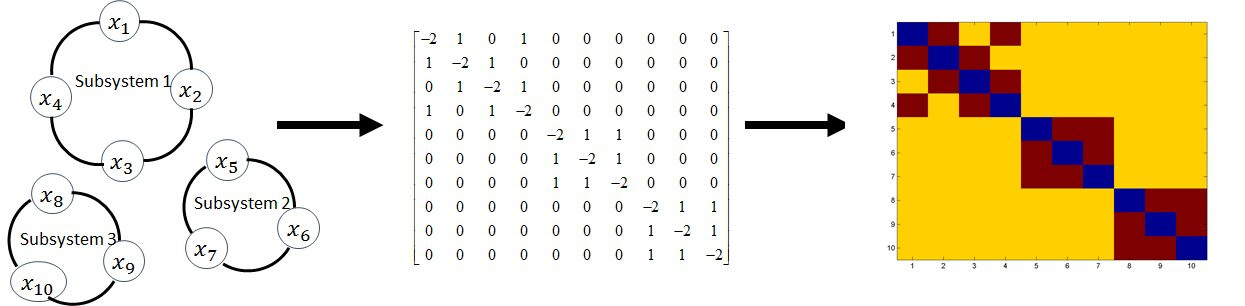
\includegraphics[width=\textwidth]{figures/FIG_10}
        \caption{Example of 10-dimensional informed agent system. The system comprises of subsystems of 3-4 states which are diffusively coupled}
        \label{linsyst}
\end{figure}

\begin{figure}[H]
        \centering
        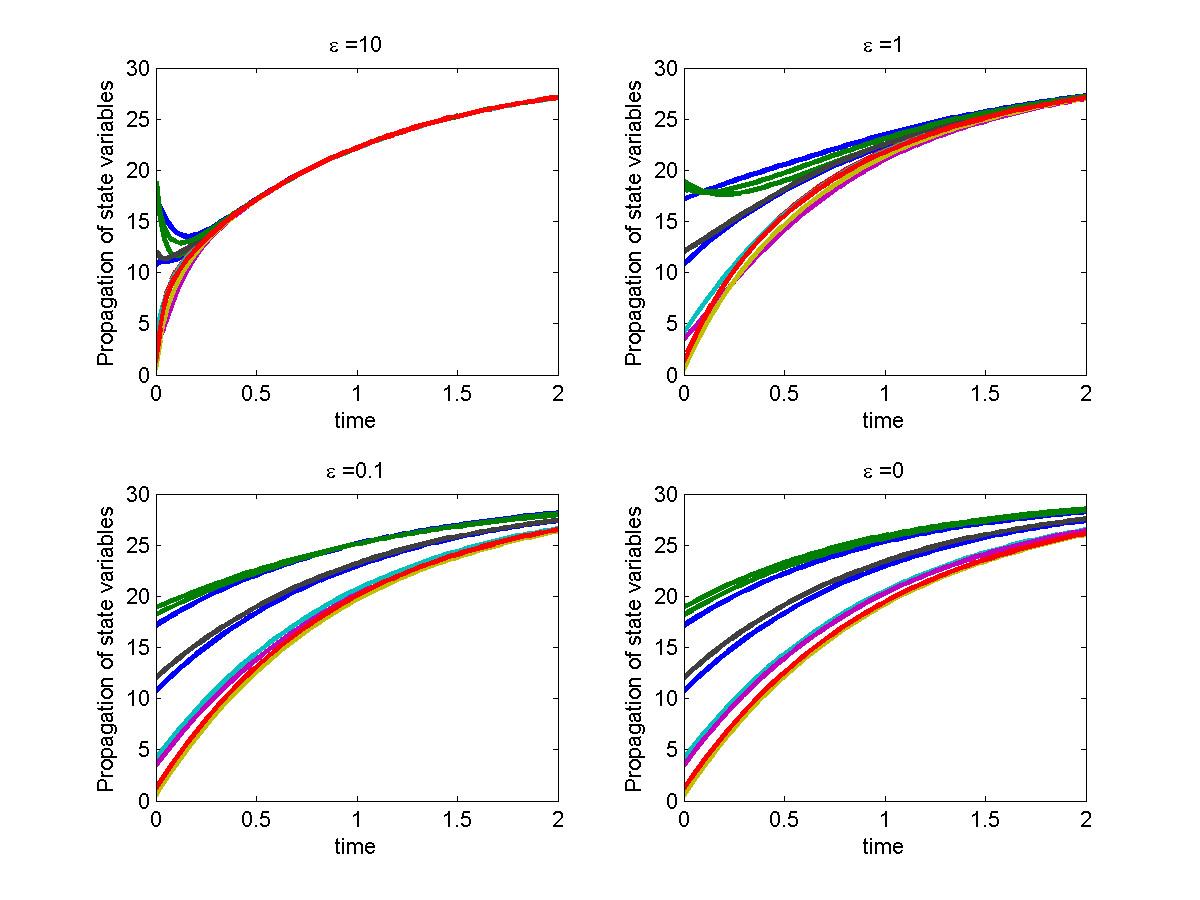
\includegraphics[width=\textwidth]{figures/FIG_11}
        \caption{Propagation of 10-dimensional coupled system with different values of $\epsilon$}\label{linsysts}
\end{figure}

However, the final $A$ matrix structure will depend on the value of $\epsilon$. While high value of $\epsilon_i$ will enforce the coupling between the oscillators, a very low value of $\epsilon$ will allow the algorithm to identify the system as a set of decoupled oscillators. The steady state solution of the individual states with $\epsilon = 0$, is $x_i^* = a_i$. The steady state solution for the whole system is given by,
\begin{equation}
\textbf{x}^* = -A^{-1}a = -(\epsilon G - \textbf{I})^{-1}a
\end{equation}

The sum of each row of $A$ is -1. Hence, an Eigenvalue of $A$ and $A^{-1}$ is -1. The corresponding Eigenvector is the null-space of the matrix $G$, which is $\textbf{1}_{n \times 1}$. Thus, the state solution for the system is also $\textbf{x}^* = a$.
Let us check the propagation of a 10-dimensional system, that is fully coupled with no subsystem present, under different values of $\epsilon$ and $a = 30\cdot\textbf{1}_{n  \times 1}$. Figure~\ref{linsysts} shows the propagation of the coupled 10-dimensional system with the same initial condition. It is seen that the system becomes almost completely \textit{synchronized} with a high value of $\epsilon$. As the value decreases, the \textit{phase-locking} also vanishes and the states behave as if they are decoupled. The value of $\epsilon$ controls the rate at which the states reach the steady-state solution. 

Next, the assemblies of different subsystems have been taken up to form large systems of higher order. The clustering techniques on the systems have been applied to identify the decoupled subsystems. The identified cluster structure does not depend on the time interval or the initial condition uncertainty. Hence, there is no need to apply the linearization techniques. The dimension of the overall system, the number of subsystems, and the number of clusters (or subsystems) identified by the two clustering techniques are given in Table~\ref{linsyst_table}. 

\begin{table}[H]
\centering
\scriptsize{
\caption{Dimension of overall system, number of subsystems, and the number of clusters identified by the different clustering techniques}
\label{linsyst_table}
\begin{tabular}{|c|c|c|c|c|c|c|c|}
\hline 
\multirow{2}{*}{$n$} & $m$ & $m$ & $m$ & \multirow{2}{*}{$n$} & $m$ & $m$ & $m$ \\ \cline{2-4} \cline{6-8} 
& Expected & with SC & with NMF & & Expected & with SC & with NMF \\ \hline
20    &    5    &    5    &    5    &    200    &    50    &    50    &    50    \\ \hline
30    &    7    &    7    &    7    &    300    &    75    &    75    &    75    \\ \hline
40    &    10    &    10    &    10    &    400    &    100    &    100    &    100    \\ \hline
50    &    12    &    12    &    12    &    500    &    125    &    125    &    125    \\ \hline
60    &    15    &    15    &    15    &    600    &    150    &    150    &    150    \\ \hline
70    &    17    &    17    &    17    &    700    &    175    &    175    &    175    \\ \hline
80    &    20    &    20    &    20    &    800    &    200    &    200    &    200    \\ \hline
90    &    22    &    22    &    22    &    900    &    225    &    225    &    225    \\ \hline
100    &    25    &    25    &    25    &    1000    &    250    &    250    &    250    \\ \hline
\end{tabular}
} 
\end{table}

The values show that both the clustering methods are equally efficient in identifying the correct number of subsystems. However, the efficiency in finding out the right cluster structure is not evident from these values. 

\begin{figure}[H]
        \centering
        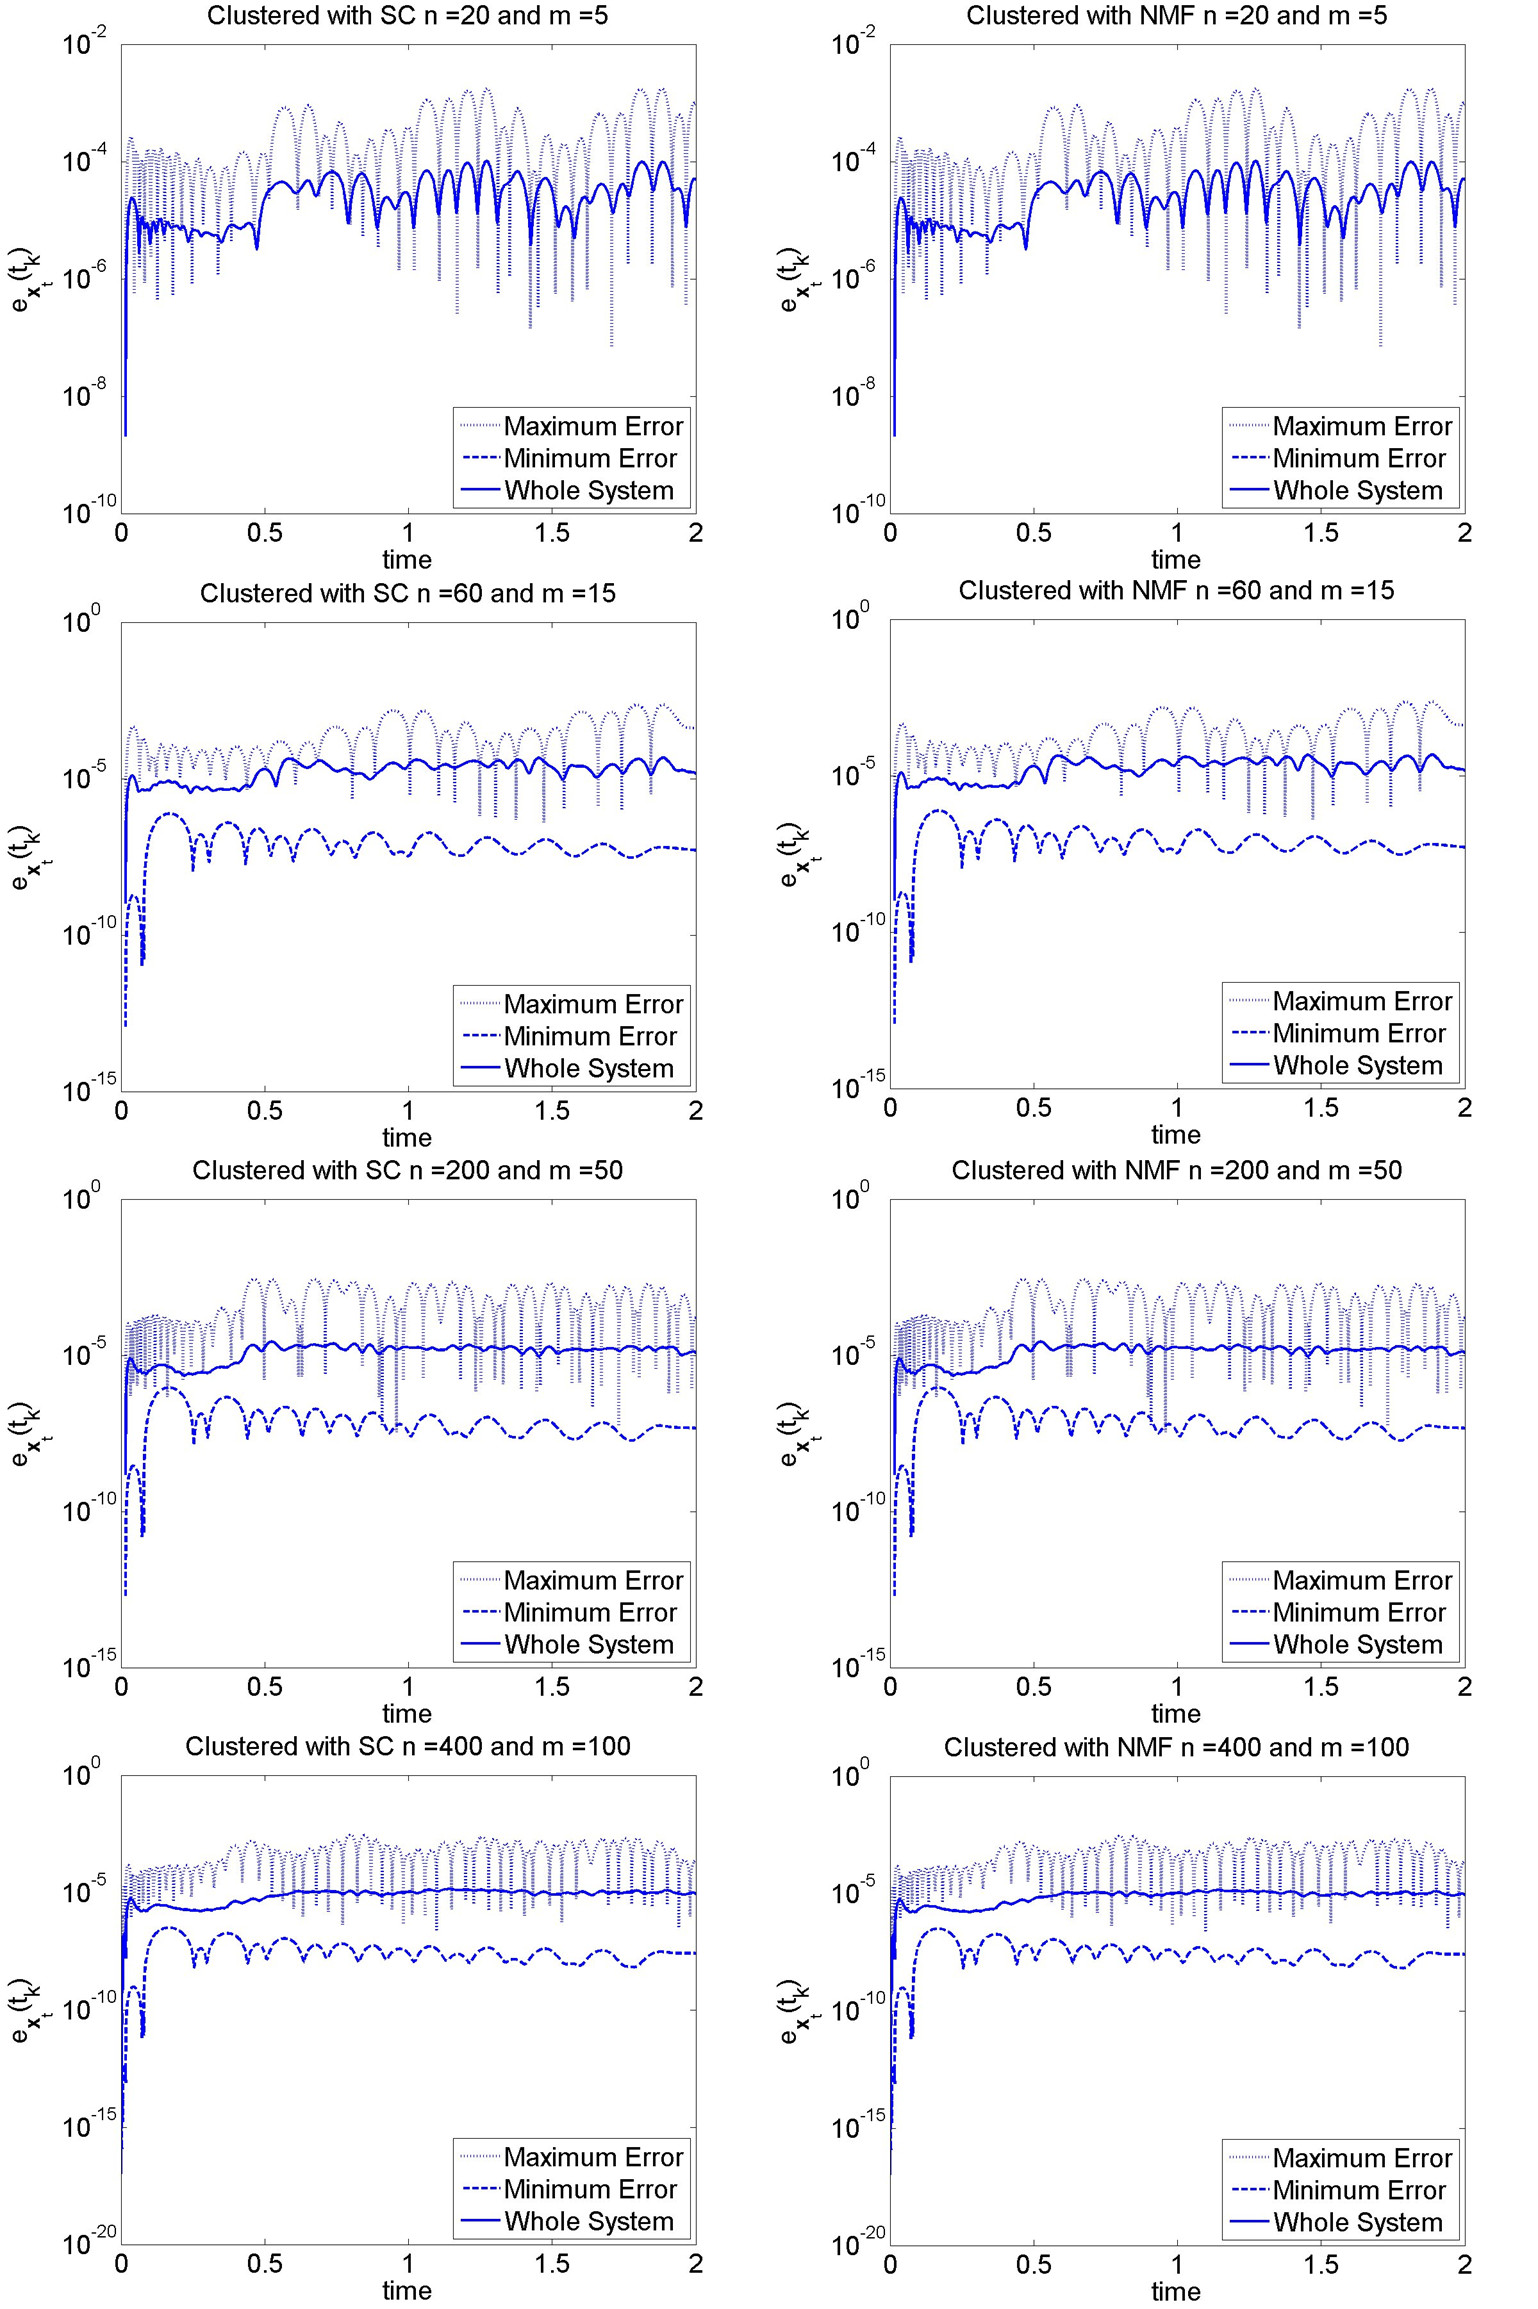
\includegraphics[width=\textwidth,height=\textwidth]{figures/FIG_12}
        \caption{Propagation of the coupled linear system for different size of problems}
        \label{linsyst_prop}
\end{figure}

Next, some random initial conditions have been taken up and used to propagate both the original system and the clustered model obtained by the two clustering methods. The comparison of the trajectory gives us a clear idea about the accuracy of the clustering methods. Figure~\ref{linsyst_prop} shows the plot of error in propagation in terms of $e_\textbf{x}(t_k)$ vs time of the linear system for different dimensions. For each system we have calculated the time-averaged error for each of the cluster as $\bar{e} = \int e_\textbf{x}(t_k) dt_k$. The `Maximum Error' and the `Minimum Error' plot corresponds to the error propagation plot for those clusters with the maximum and minimum values of $\bar{e}$. It can be observed that with $n = 20$, the minimum error value for a cluster is 0. The error range for the whole system is between $10^{-7}$ and $10^{-4}$. The error range for the system is fairly constant for different dimensions of the problems. Also, there is no such discernible variation in the error for the `Maximum Error' and the `Minimum Error' plots for the different problems. This observation speaks of the robustness of the method of clustering to the size of the problem. 

\subsection{Weakly Coupled Van der Pol Oscillators}
Let us consider the second order differential equation of $N$ nonidentical and decoupled unforced Van der Pol oscillators~\cite{van1920theory} given as, 
\begin{equation}
\ddot{x}_i - \nu_i (1-x_i^2) \dot{x} + x_i = 0
\end{equation}
with a nonlinear damping function controlled by a single parameter $\nu_i$ and linear stiffness. The state space  formulation can be written as,
\begin{equation}
\label{weak_vanderpol}
\begin{array}{l}
\dot{x}_i = y_i + \epsilon (x_{i-1} - 2x_i + x_{i+1}) \\
\dot{y}_i = \nu_i(1-x_i^2)y_i - x_i  
\end{array}\hspace{5 mm} i = 1,2,\ldots,N
\end{equation}
The undamped equation of this model represents the equation of a simple harmonic oscillator, while a positive value of $\nu_i$'s forces the individual systems to enter into a limit cycle oscillation. Analysis shows that, $x_i = [0 \; 0]^T$ is an unstable equilibrium point. Let us now study the behavior of the system under Statistical Linearization for a system with $\epsilon = 0$, $N = 5$ with random value of mean $\mu = [0.2, 0.2, \ldots, 0.2]$ and covariance $ \alpha \Sigma$, where 
\begin{equation}
\Sigma = \begin{bmatrix}
1 & 0.1 & 0.1 & 0.1 & 0.1 & 0.1 & 0 & 0 & 0 & 0 \\
0.1 & 1 & 0.1 & 0.1 & 0.1 & 0.1 & 0 & 0 & 0 & 0 \\
\vdots & \vdots & &  & \ddots & & \ddots    & & \vdots & \vdots \\
0 & 0 & 0 & 0 & 0 & 0 & 0.1 & 0.1 & 1 & 0.1 \\
0 & 0 & 0 & 0 & 0 & 0 & 0.1 & 0.1 & 0.1 & 1 \\
\end{bmatrix}
\end{equation}
\noindent The time-dependent linearization technique is independent of the value of $\alpha$. To show the change in Statistically linearized matrix $A_{sl}$, the value of $\alpha$ is varied. Figure~\ref{statlinsysts} shows the color image of $A_{sl}$ computed using different values of $\alpha$. The plot shows that the matrix $A_{sl}$ is capable of capturing the effect of the covariance values. With higher values of $\alpha$, the two different blocks of the covariance matrix is captured by the matrix $A_{sl}$. Intuitively, it can be inferred that, the time-based linearization is unable to capture these blocks. Next, we take up several such initial conditions for the purpose of further experimentation. The system has been linearized and the state space has been decomposed based on each of the initial conditions and the dynamics of the system. Table~\ref{weakvanderpol} shows the average mean and covariance of error in propagation obtained for the seven methods for some of the test cases. All the methods consistently show low error values for all of the test cases. A few percentage of the error values are in the range of $10^{-1}$, while maximum error values are in the range of $10^{-7}$ or $10^{-10}$. There is a need of a detailed statistical analysis so as to get a deeper insight into the test results. 

\begin{figure}[H]
        \centering
        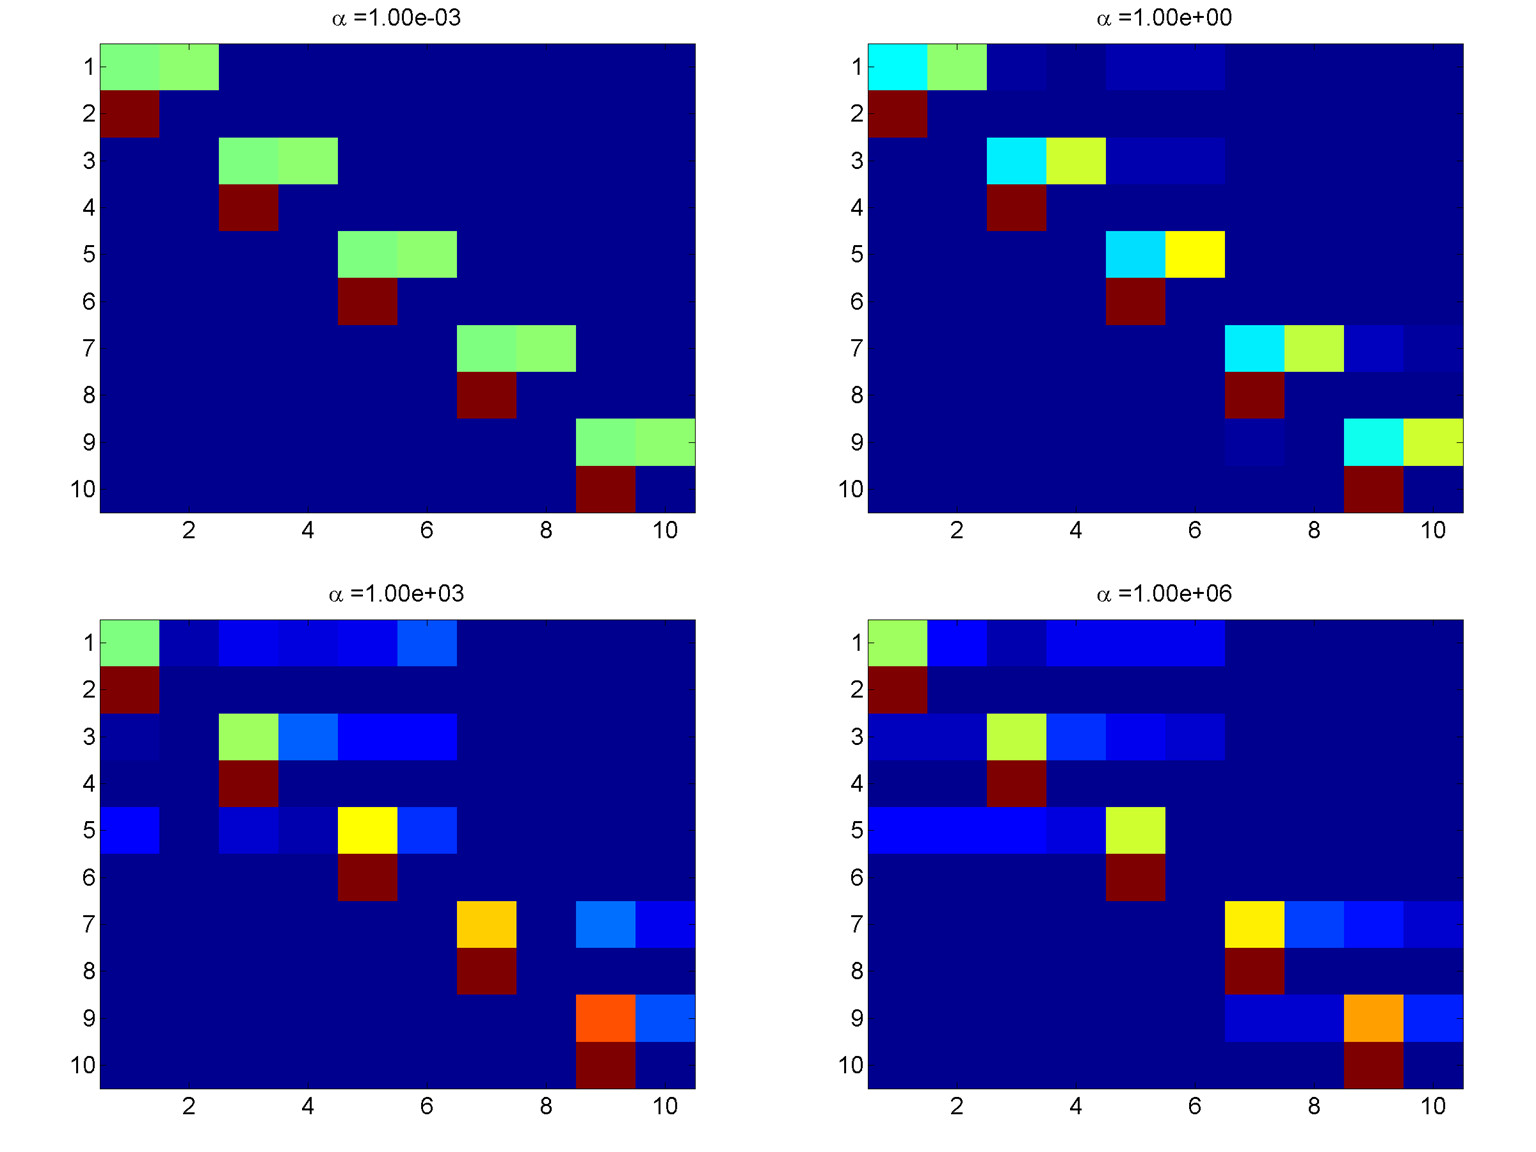
\includegraphics[width=\textwidth]{figures/FIG_13}
        \caption{Variation in $A_{sl}$ of 10-dimensional coupled oscillator system with different values of $\alpha$}
        \label{statlinsysts}
\end{figure}

\begin{table}[H]
\caption{RMS \textit{time-averaged} mean and \textit{time-averaged} covariance for different test setups in Weakly Coupled Van der Pol Oscillators}
\begin{center}
\resizebox{\columnwidth}{!}{
\label{weakvanderpol}
\begin{tabular}{|c|c|c|c|c|c|c|c|c|c|c|c|c|c|c|c|}
\hline 
\multirow{2}{*}{$n$} & \multirow{2}{*}{$e$} &  \multicolumn{2}{c|}{Method I}  & \multicolumn{2}{c|}{Method II} & \multicolumn{2}{c|}{Method III} & \multicolumn{2}{c|}{Method I} & \multicolumn{2}{c|}{Method III} & \multicolumn{2}{c|}{SL} & \multicolumn{2}{c|}{SL} \\ \cline{3-16}
                        &                         & \multicolumn{2}{c|}{ + SC}     &   \multicolumn{2}{c|}{ + SC}    &    \multicolumn{2}{c|}{ + SC}    &   \multicolumn{2}{c|}{ + NMF}  &  \multicolumn{2}{c|}{ + NMF}  & \multicolumn{2}{c|}{ + SC}  &  \multicolumn{2}{c|}{ + NMF} \\ \hline
10    &    0.00E+00    &    4.88E-02    &    6.22E-02    &    4.80E-02    &    6.18E-02    &    4.88E-02    &    6.22E-02    &    4.70E-02    &    6.13E-02    &    4.71E-02    &    6.13E-02    &    1.18E-06    &    3.56E-04    &    4.75E-02    &    5.96E-02    \\ \hline
10    &    1.00E-01    &    2.48E-02    &    4.28E-02    &    2.57E-02    &    4.71E-02    &    2.48E-02    &    4.28E-02    &    2.77E-02    &    5.58E-02    &    2.71E-02    &    5.07E-02    &    2.48E-02    &    4.28E-02    &    3.21E-02    &    5.71E-02    \\ \hline
10    &    1.00E-02    &    2.34E-02    &    4.15E-02    &    2.46E-02    &    4.63E-02    &    2.34E-02    &    4.13E-02    &    2.65E-02    &    5.33E-02    &    2.62E-02    &    5.25E-02    &    2.34E-02    &    4.14E-02    &    3.01E-02    &    5.62E-02    \\ \hline
10    &    1.00E-03    &    6.18E-02    &    6.49E-02    &    5.89E-02    &    6.09E-02    &    5.42E-02    &    5.29E-02    &    6.11E-02    &    6.56E-02    &    6.00E-02    &    6.56E-02    &    5.42E-02    &    5.29E-02    &    5.98E-02    &    6.53E-02    \\ \hline
10    &    1.00E-04    &    5.30E-02    &    6.53E-02    &    5.01E-02    &    6.09E-02    &    4.70E-02    &    5.39E-02    &    5.17E-02    &    6.49E-02    &    5.24E-02    &    6.50E-02    &    4.71E-02    &    5.37E-02    &    5.32E-02    &    6.52E-02    \\ \hline
10    &    1.00E-05    &    5.01E-02    &    6.52E-02    &    4.83E-02    &    6.13E-02    &    4.60E-02    &    5.72E-02    &    4.96E-02    &    6.47E-02    &    5.00E-02    &    6.49E-02    &    4.41E-02    &    5.16E-02    &    4.98E-02    &    6.43E-02    \\ \hline
10    &    1.00E-06    &    4.24E-02    &    6.09E-02    &    4.13E-02    &    5.86E-02    &    4.19E-02    &    5.99E-02    &    4.17E-02    &    6.06E-02    &    4.23E-02    &    6.06E-02    &    3.78E-02    &    4.86E-02    &    4.42E-02    &    6.14E-02    \\ \hline
10    &    1.00E-07    &    4.45E-02    &    6.15E-02    &    4.33E-02    &    5.93E-02    &    4.44E-02    &    6.14E-02    &    4.36E-02    &    6.11E-02    &    4.41E-02    &    6.11E-02    &    3.90E-02    &    4.93E-02    &    4.52E-02    &    6.22E-02    \\ \hline
20    &    0.00E+00    &    6.36E-05    &    6.56E-03    &    6.35E-05    &    6.56E-03    &    6.36E-05    &    6.56E-03    &    8.69E-05    &    7.03E-03    &    7.51E-05    &    6.60E-03    &    1.01E-04    &    6.84E-03    &    6.08E-05    &    6.53E-03    \\ \hline
20    &    1.00E-01    &    2.13E-07    &    2.73E-06    &    1.03E-02    &    1.54E-02    &    6.34E-02    &    5.99E-02    &    3.03E-02    &    4.12E-02    &    2.15E-02    &    3.57E-02    &    3.49E-09    &    8.75E-08    &    2.67E-02    &    3.84E-02    \\ \hline
20    &    1.00E-02    &    2.91E-02    &    9.51E-02    &    1.14E-02    &    1.61E-02    &    3.02E-02    &    6.15E-02    &    3.03E-02    &    4.11E-02    &    2.69E-02    &    3.96E-02    &    0.00E+00    &    7.93E-02    &    2.64E-02    &    3.84E-02    \\ \hline
20    &    1.00E-03    &    1.06E-01    &    8.49E-02    &    1.19E-02    &    1.64E-02    &    2.85E-02    &    1.33E-01    &    3.02E-02    &    4.11E-02    &    2.95E-02    &    4.08E-02    &    0.00E+00    &    1.08E-01    &    2.63E-02    &    3.84E-02    \\ \hline
20    &    1.00E-04    &    9.26E-02    &    2.44E-02    &    1.21E-02    &    1.65E-02    &    6.54E-03    &    4.65E-02    &    3.02E-02    &    4.11E-02    &    3.03E-02    &    4.11E-02    &    0.00E+00    &    1.07E-01    &    2.63E-02    &    3.84E-02    \\ \hline
20    &    1.00E-05    &    6.54E-03    &    6.54E-03    &    1.21E-02    &    1.65E-02    &    3.52E-02    &    6.61E-02    &    3.02E-02    &    4.10E-02    &    3.03E-02    &    4.11E-02    &    0.00E+00    &    6.54E-03    &    2.64E-02    &    3.84E-02    \\ \hline
20    &    1.00E-06    &    1.04E-01    &    6.82E-02    &    1.21E-02    &    1.64E-02    &    7.12E-02    &    1.06E-01    &    3.01E-02    &    4.10E-02    &    3.02E-02    &    4.11E-02    &    0.00E+00    &    3.43E-02    &    2.63E-02    &    3.84E-02    \\ \hline
20    &    1.00E-07    &    4.04E-02    &    1.05E-01    &    1.20E-02    &    1.64E-02    &    1.17E-01    &    1.32E-01    &    3.01E-02    &    4.10E-02    &    3.02E-02    &    4.10E-02    &    0.00E+00    &    4.62E-02    &    2.63E-02    &    3.84E-02    \\ \hline
50    &    0.00E+00    &    1.27E-02    &    1.80E-02    &    1.26E-02    &    1.80E-02    &    4.11E-02    &    1.80E-02    &    1.24E-02    &    1.79E-02    &    1.24E-02    &    1.79E-02    &    1.09E-07    &    5.68E-05    &    1.13E-02    &    1.73E-02    \\ \hline
50    &    1.00E-01    &    7.86E-02    &    3.66E-02    &    3.94E-03    &    6.69E-03    &    7.99E-02    &    1.01E-01    &    1.12E-02    &    1.72E-02    &    8.10E-03    &    1.57E-02    &    8.10E-03    &    1.57E-02    &    1.02E-02    &    1.65E-02    \\ \hline
50    &    1.00E-02    &    3.35E-02    &    2.45E-02    &    4.46E-03    &    7.04E-03    &    6.54E-03    &    1.66E-02    &    1.16E-02    &    1.75E-02    &    1.04E-02    &    1.71E-02    &    1.04E-02    &    1.71E-02    &    1.05E-02    &    1.69E-02    \\ \hline
50    &    1.00E-03    &    4.67E-03    &    2.59E-02    &    4.13E-03    &    6.75E-03    &    4.77E-02    &    7.46E-02    &    1.03E-02    &    1.69E-02    &    1.00E-02    &    1.67E-02    &    1.00E-02    &    1.67E-02    &    9.26E-03    &    1.61E-02    \\ \hline
50    &    1.00E-04    &    1.76E-02    &    9.85E-02    &    4.90E-03    &    7.24E-03    &    4.86E-02    &    5.67E-02    &    1.21E-02    &    1.78E-02    &    1.20E-02    &    1.77E-02    &    1.20E-02    &    1.77E-02    &    1.09E-02    &    1.71E-02    \\ \hline
50    &    1.00E-05    &    1.38E-03    &    5.76E-02    &    3.53E-04    &    3.26E-03    &    0.00E+00    &    9.66E-03    &    9.18E-04    &    8.43E-03    &    9.20E-04    &    8.41E-03    &    9.20E-04    &    8.41E-03    &    8.63E-04    &    7.68E-03    \\ \hline
50    &    1.00E-06    &    5.42E-02    &    8.06E-02    &    5.20E-04    &    3.81E-03    &    0.00E+00    &    7.90E-02    &    1.45E-03    &    9.64E-03    &    1.44E-03    &    9.63E-03    &    1.44E-03    &    9.63E-03    &    1.27E-03    &    8.76E-03    \\ \hline
50    &    1.00E-07    &    6.50E-02    &    6.97E-02    &    4.61E-03    &    6.95E-03    &    0.00E+00    &    0.00E+00    &    1.16E-02    &    1.76E-02    &    1.16E-02    &    1.76E-02    &    1.16E-02    &    1.76E-02    &    1.05E-02    &    1.69E-02    \\ \hline
100    &    0.00E+00    &    6.54E-03    &    9.36E-03    &    6.48E-03    &    9.35E-03    &    6.54E-03    &    9.36E-03    &    6.41E-03    &    9.34E-03    &    6.42E-03    &    9.34E-03    &    7.06E-03    &    9.40E-03    &    5.99E-03    &    9.12E-03    \\ \hline
100    &    1.00E-01    &    1.95E-02    &    2.47E-02    &    4.46E-03    &    7.04E-03    &    0.00E+00    &    0.00E+00    &    0.00E+00    &    0.00E+00    &    0.00E+00    &    0.00E+00    &    0.00E+00    &    0.00E+00    &    0.00E+00    &    0.00E+00    \\ \hline
100    &    1.00E-02    &    8.78E-02    &    7.47E-02    &    4.13E-03    &    6.75E-03    &    0.00E+00    &    0.00E+00    &    0.00E+00    &    0.00E+00    &    0.00E+00    &    0.00E+00    &    0.00E+00    &    0.00E+00    &    0.00E+00    &    0.00E+00    \\ \hline
100    &    1.00E-03    &    4.18E-02    &    3.85E-02    &    2.94E-04    &    2.29E-03    &    0.00E+00    &    0.00E+00    &    7.53E-04    &    5.63E-03    &    7.46E-04    &    5.56E-03    &    0.00E+00    &    0.00E+00    &    6.19E-04    &    4.85E-03    \\ \hline
100    &    1.00E-04    &    5.42E-03    &    6.11E-02    &    6.86E-04    &    2.81E-03    &    0.00E+00    &    0.00E+00    &    1.67E-03    &    6.71E-03    &    1.66E-03    &    6.69E-03    &    0.00E+00    &    0.00E+00    &    1.41E-03    &    5.97E-03    \\ \hline
100    &    1.00E-05    &    7.49E-02    &    3.30E-02    &    2.76E-04    &    2.24E-03    &    0.00E+00    &    0.00E+00    &    7.19E-04    &    5.58E-03    &    7.18E-04    &    5.57E-03    &    0.00E+00    &    0.00E+00    &    5.92E-04    &    4.81E-03    \\ \hline
100    &    1.00E-06    &    3.03E-04    &    4.86E-03    &    3.03E-04    &    4.86E-03    &    3.07E-04    &    4.83E-03    &    3.06E-04    &    4.87E-03    &    3.18E-04    &    4.89E-03    &    3.42E-04    &    4.87E-03    &    3.19E-04    &    4.88E-03    \\ \hline
100    &    1.00E-07    &    3.03E-04    &    4.86E-03    &    3.03E-04    &    4.86E-03    &    3.07E-04    &    4.85E-03    &    3.06E-04    &    4.87E-03    &    3.28E-04    &    4.91E-03    &    3.42E-04    &    4.87E-03    &    3.19E-04    &    4.88E-03    \\ \hline
150    &    0.00E+00    &    4.33E-03    &    6.32E-03    &    4.30E-03    &    6.32E-03    &    4.33E-03    &    6.32E-03    &    4.26E-03    &    6.31E-03    &    4.26E-03    &    6.31E-03    &    4.61E-03    &    6.35E-03    &    4.09E-03    &    6.21E-03    \\ \hline
150    &    1.00E-01    &    1.68E-02    &    4.99E-02    &    1.06E-04    &    1.38E-03    &    1.48E-01    &    1.15E-01    &    6.27E-02    &    2.09E-02    &    3.47E-04    &    3.11E-03    &    0.00E+00    &    0.00E+00    &    1.56E-04    &    2.51E-03    \\ \hline
150    &    1.00E-02    &    9.97E-03    &    7.75E-02    &    1.27E-04    &    1.59E-03    &    1.26E-01    &    9.84E-02    &    4.95E-02    &    3.51E-02    &    3.07E-04    &    3.59E-03    &    0.00E+00    &    0.00E+00    &    1.43E-04    &    2.84E-03    \\ \hline
150    &    1.00E-03    &    4.68E-03    &    8.83E-02    &    6.11E-05    &    1.24E-03    &    2.49E-01    &    2.32E-01    &    1.63E-01    &    1.78E-01    &    1.22E-01    &    1.70E-01    &    3.69E-02    &    1.25E-01    &    1.66E-02    &    9.36E-02    \\ \hline
150    &    1.00E-04    &    5.07E-02    &    1.01E-02    &    0.00E+00    &    0.00E+00    &    1.84E-01    &    1.53E-01    &    1.34E-01    &    1.31E-01    &    1.04E-01    &    1.02E-01    &    9.53E-02    &    3.94E-02    &    6.70E-03    &    8.09E-03    \\ \hline
150    &    1.00E-05    &    -2.95E-03    &    5.22E-02    &    0.00E+00    &    0.00E+00    &    2.11E-01    &    2.57E-01    &    1.93E-01    &    2.07E-01    &    1.37E-01    &    1.32E-01    &    9.73E-02    &    9.50E-02    &    3.45E-03    &    4.26E-02    \\ \hline
150    &    1.00E-06    &    7.41E-02    &    2.01E-02    &    0.00E+00    &    0.00E+00    &    2.33E-01    &    2.60E-01    &    2.02E-01    &    1.65E-01    &    1.29E-01    &    1.56E-01    &    1.27E-01    &    1.01E-01    &    9.06E-02    &    4.28E-02    \\ \hline
150    &    1.00E-07    &    6.14E-02    &    2.16E-02    &    0.00E+00    &    0.00E+00    &    2.11E-01    &    2.37E-01    &    1.95E-01    &    2.24E-01    &    1.97E-01    &    1.82E-01    &    1.10E-01    &    9.90E-02    &    4.67E-02    &    6.61E-02    \\ \hline
200    &    0.00E+00    &    4.70E-02    &    9.18E-02    &    0.00E+00    &    0.00E+00    &    1.10E-01    &    2.62E-01    &    5.24E-02    &    2.22E-01    &    2.43E-02    &    1.86E-01    &    2.33E-02    &    1.19E-01    &    2.77E-03    &    2.86E-02    \\ \hline
200    &    1.00E-01    &    2.24E-02    &    9.40E-02    &    3.77E-05    &    8.50E-04    &    2.44E-01    &    2.80E-01    &    1.86E-01    &    2.52E-01    &    1.17E-01    &    1.90E-01    &    5.55E-02    &    1.26E-01    &    7.34E-03    &    3.29E-02    \\ \hline
200    &    1.00E-02    &    5.99E-02    &    4.59E-02    &    3.94E-05    &    9.98E-04    &    2.83E-01    &    2.34E-01    &    2.02E-01    &    2.29E-01    &    1.44E-01    &    1.87E-01    &    1.27E-01    &    1.10E-01    &    3.44E-02    &    8.07E-02    \\ \hline
200    &    1.00E-03    &    6.63E-02    &    7.12E-02    &    1.06E-05    &    3.32E-04    &    2.52E-01    &    3.16E-01    &    2.23E-01    &    3.11E-01    &    1.53E-01    &    2.30E-01    &    1.29E-01    &    1.45E-01    &    5.53E-02    &    5.50E-02    \\ \hline
200    &    1.00E-04    &    8.42E-02    &    1.01E-02    &    0.00E+00    &    0.00E+00    &    3.90E-01    &    2.18E-01    &    3.19E-01    &    1.61E-01    &    2.53E-01    &    1.30E-01    &    1.78E-01    &    8.22E-02    &    8.38E-02    &    6.46E-02    \\ \hline
200    &    1.00E-05    &    5.10E-02    &    3.21E-02    &    3.04E-05    &    8.50E-04    &    1.41E-01    &    1.95E-01    &    5.22E-02    &    1.94E-01    &    4.27E-02    &    1.65E-01    &    3.17E-02    &    1.50E-01    &    -3.24E-03    &    7.86E-02    \\ \hline
200    &    1.00E-06    &    4.91E-02    &    3.94E-02    &    0.00E+00    &    0.00E+00    &    1.61E-01    &    1.67E-01    &    1.16E-01    &    9.53E-02    &    1.06E-01    &    8.81E-02    &    8.17E-02    &    4.77E-02    &    2.38E-02    &    4.42E-02    \\ \hline
200    &    1.00E-07    &    9.03E-03    &    6.95E-02    &    4.65E-06    &    3.48E-04    &    2.02E-01    &    2.25E-01    &    1.48E-01    &    1.44E-01    &    7.26E-02    &    1.46E-01    &    6.45E-02    &    9.41E-02    &    1.55E-03    &    7.19E-02    \\ \hline
\end{tabular} 
}
\end{center}
\end{table}

\subsection{Weakly Coupled Lorenz Attractors}

Let us consider the equation of $N$ nonidentical and decoupled Lorenz attractors~\cite{lorenz1963deterministic}, where the $i^{th}$ oscillator is defined by the system of following differential equation,  
\begin{equation}
\begin{array}{lc}
\dot{x}_{i} = \sigma_i (y_{i} - x_{i}) + \epsilon (x_{i+1} + x_{i-1} - 2x_{ti})  \\
\dot{y}_{i} = x_{i}(\rho_i - z_i) - y_{i} \\
\dot{z}_{i} = x_{i}y_{i} - \beta z_{i} & \hspace{5 mm}
i = 1,2,\ldots,N
\end{array} 
\end{equation} %\epsilon (x_{i+1} + x_{i-1} - 2x_{ti})

Intuitively, we can conclude that the system comprises of $N$ clusters. We have applied the methodology described in Sections~\ref{wcs:linearization} and~\ref{non_overlap_clustering} to linearize and cluster the state space and estimate the uncertainties associated with each of the variables. In this example also, to show the performance and the accuracy of the clustering method, we have made a comparison between the trajectories of the propagation of the original system, and that of the clustered model. Lorenz attractors exhibit chaotic properties for certain parameters. With $e = 0$, the equilibrium point for any set of parameters for an individual oscillator is $[0 \; 0 \; 0]^T$. With slight perturbation, the system repels from the equilibrium point and orients itself around two steady convection given by $\left( \pm\sqrt{\beta(\rho-1)}, \pm\sqrt{\beta(\rho-1)}, \rho-1 \right)$. Table~\ref{weaklorenz} shows the average mean and covariance of error in propagation obtained for the seven methods for some of the test cases. Lorenz system is a highly chaotic system. Hence, any slight error in wrong cluster detection can lead to huge error. Also, the cluster structure is periodically updated, which implies that any wrong cluster detection at an earlier time will result in a huge cumulative error at the end of the overall propagation. 

\begin{table}[H]
\caption{RMS \textit{time-averaged} mean and \textit{time-averaged} covariance for different test setups in Weakly Coupled Lorenz Attractors}
\begin{center}
\resizebox{\columnwidth}{!}{
\label{weaklorenz}
\begin{tabular}{|c|c|c|c|c|c|c|c|c|c|c|c|c|c|c|c|}
\hline 
\multirow{2}{*}{$n$} & \multirow{2}{*}{$e$} &  \multicolumn{2}{c|}{Method I}  & \multicolumn{2}{c|}{Method II} & \multicolumn{2}{c|}{Method III} & \multicolumn{2}{c|}{Method I} & \multicolumn{2}{c|}{Method III} & \multicolumn{2}{c|}{SL} & \multicolumn{2}{c|}{SL} \\ \cline{3-16}
                        &                         & \multicolumn{2}{c|}{ + SC}     &   \multicolumn{2}{c|}{ + SC}    &    \multicolumn{2}{c|}{ + SC}    &   \multicolumn{2}{c|}{ + NMF}  &  \multicolumn{2}{c|}{ + NMF}  & \multicolumn{2}{c|}{ + SC}  &  \multicolumn{2}{c|}{ + NMF} \\ \hline
15    &    1.00E-01    &    2.31E+00    &    3.29E-01    &    2.32E+00    &    3.38E-01    &    4.22E+00    &    2.88E+00    &    4.25E+00    &    3.03E+00    &    3.22E+01    &    3.66E+00    &    9.38E-07    &    2.18E-06    &    1.71E-01    &    8.40E-02    \\ \hline
15    &    1.00E-02    &    6.11E+01    &    1.62E+01    &    6.05E+01    &    1.54E+01    &    2.01E+02    &    6.23E+01    &    2.09E+02    &    6.53E+01    &    1.21E+02    &    2.38E+01    &    1.27E+02    &    1.04E+02    &    1.22E+02    &    1.07E+02    \\ \hline
15    &    1.00E-03    &    6.57E+01    &    1.81E+01    &    6.91E+01    &    1.75E+01    &    2.37E+02    &    7.09E+01    &    2.45E+02    &    6.83E+01    &    1.07E+02    &    2.64E+01    &    1.29E+02    &    1.01E+02    &    1.34E+02    &    1.02E+02    \\ \hline
15    &    1.00E-04    &    7.45E+01    &    1.78E+01    &    7.38E+01    &    1.77E+01    &    2.13E+02    &    6.69E+01    &    2.10E+02    &    6.59E+01    &    7.05E+01    &    1.57E+01    &    1.36E+02    &    9.03E+01    &    1.37E+02    &    9.37E+01    \\ \hline
15    &    1.00E-05    &    5.21E+01    &    1.68E+01    &    5.08E+01    &    1.73E+01    &    1.74E+02    &    5.63E+01    &    1.72E+02    &    5.43E+01    &    6.09E+01    &    1.59E+01    &    8.74E+01    &    7.19E+01    &    9.12E+01    &    6.87E+01    \\ \hline
15    &    1.00E-06    &    3.40E+01    &    1.39E+01    &    3.56E+01    &    1.34E+01    &    2.93E+02    &    6.47E+01    &    2.84E+02    &    6.78E+01    &    1.92E+02    &    6.32E+01    &    2.71E+02    &    6.55E+01    &    2.70E+02    &    6.27E+01    \\ \hline
15    &    1.00E-07    &    6.44E+01    &    2.50E+01    &    6.56E+01    &    2.42E+01    &    1.78E+02    &    5.59E+01    &    1.76E+02    &    5.43E+01    &    8.38E+01    &    1.65E+01    &    1.14E+02    &    8.13E+01    &    1.11E+02    &    8.51E+01    \\ \hline
30    &    0.00E+00    &    2.40E-02    &    1.21E-02    &    3.08E-01    &    5.59E-02    &    2.40E-02    &    1.21E-02    &    2.20E-01    &    5.40E-02    &    2.93E-01    &    5.58E-02    &    1.02E-04    &    3.54E-05    &    1.55E-02    &    7.17E-03    \\ \hline
30    &    1.00E-01    &    9.39E+01    &    9.97E+00    &    9.60E+01    &    9.82E+00    &    1.57E+02    &    3.40E+01    &    1.58E+02    &    3.25E+01    &    2.50E+02    &    1.05E+02    &    3.69E+01    &    5.88E+00    &    3.60E+01    &    5.84E+00    \\ \hline
30    &    1.00E-02    &    6.40E+01    &    3.63E+01    &    6.53E+01    &    3.72E+01    &    3.45E+02    &    2.50E+02    &    3.32E+02    &    2.51E+02    &    5.22E+01    &    5.28E+00    &    7.37E+01    &    1.45E+01    &    7.15E+01    &    1.51E+01    \\ \hline
30    &    1.00E-03    &    3.16E+01    &    2.45E+01    &    3.05E+01    &    2.57E+01    &    1.31E+02    &    3.16E+01    &    1.26E+02    &    3.04E+01    &    7.55E+01    &    1.54E+01    &    3.12E+01    &    5.91E+00    &    3.12E+01    &    6.14E+00    \\ \hline
30    &    1.00E-04    &    4.44E+01    &    1.09E+01    &    4.59E+01    &    1.06E+01    &    1.80E+02    &    2.14E+01    &    1.74E+02    &    2.25E+01    &    8.78E+01    &    2.48E+01    &    1.94E+01    &    1.83E+01    &    1.89E+01    &    1.75E+01    \\ \hline
30    &    1.00E-05    &    2.44E+01    &    6.64E+00    &    2.48E+01    &    6.55E+00    &    1.22E+02    &    1.74E+01    &    1.24E+02    &    1.79E+01    &    1.16E+02    &    8.63E+01    &    7.85E+01    &    3.48E+01    &    7.63E+01    &    3.41E+01    \\ \hline
30    &    1.00E-06    &    3.03E+01    &    1.33E+01    &    3.09E+01    &    1.32E+01    &    1.98E+04    &    6.85E+03    &    1.99E+04    &    7.15E+03    &    6.85E+01    &    6.78E+01    &    1.90E+01    &    1.03E+01    &    1.99E+01    &    1.04E+01    \\ \hline
30    &    1.00E-07    &    7.75E+01    &    5.36E+01    &    7.93E+01    &    5.44E+01    &    7.59E+02    &    2.03E+02    &    7.76E+02    &    2.09E+02    &    7.92E+02    &    2.10E+02    &    1.66E+01    &    5.03E+00    &    1.68E+01    &    4.93E+00    \\ \hline
75    &    0.00E+00    &    1.01E+00    &    1.15E-01    &    1.04E+00    &    1.13E-01    &    2.92E+02    &    1.41E+02    &    2.94E+02    &    1.42E+02    &    2.04E+01    &    9.16E+00    &    4.54E-01    &    2.24E-01    &    4.69E-01    &    2.31E-01    \\ \hline
75    &    1.00E-01    &    2.47E+01    &    2.87E+00    &    2.44E+01    &    2.94E+00    &    1.58E+00    &    2.62E-01    &    1.57E+00    &    2.51E-01    &    1.34E+02    &    3.97E+01    &    3.18E+00    &    2.50E+00    &    3.11E+00    &    2.46E+00    \\ \hline
75    &    1.00E-02    &    2.18E+01    &    1.87E+01    &    2.08E+01    &    1.82E+01    &    5.67E+00    &    1.86E+00    &    5.61E+00    &    1.78E+00    &    4.63E+01    &    1.96E+01    &    1.90E+00    &    9.57E-01    &    1.99E+00    &    9.80E-01    \\ \hline
75    &    1.00E-03    &    2.77E+00    &    1.32E+00    &    2.64E+00    &    1.28E+00    &    3.78E+00    &    1.37E+00    &    3.79E+00    &    1.35E+00    &    9.08E+00    &    1.04E+00    &    4.74E+00    &    3.41E+00    &    4.78E+00    &    3.46E+00    \\ \hline
75    &    1.00E-06    &    4.78E-05    &    5.85E-06    &    4.78E-05    &    5.85E-06    &    4.74E-05    &    5.90E-06    &    4.78E-05    &    5.85E-06    &    4.78E-05    &    5.85E-06    &    4.78E-05    &    5.85E-06    &    4.78E-05    &    5.85E-06    \\ \hline
75    &    1.00E-07    &    4.78E-05    &    5.85E-06    &    4.78E-05    &    5.85E-06    &    4.74E-05    &    5.90E-06    &    4.78E-05    &    5.85E-06    &    4.78E-05    &    5.85E-06    &    4.78E-05    &    5.85E-06    &    4.78E-05    &    5.85E-06    \\ \hline
150    &    0.00E+00    &    1.75E-05    &    5.45E-05    &    2.77E+00    &    2.44E+00    &    1.75E-05    &    5.45E-05    &    4.25E+00    &    1.86E+00    &    2.11E+01    &    3.95E+00    &    1.71E-05    &    5.33E-05    &    3.74E+00    &    1.95E+00    \\ \hline
150    &    1.00E-01    &    5.89E+00    &    1.14E+00    &    6.07E+00    &    1.15E+00    &    4.57E-01    &    9.96E-02    &    4.79E-01    &    9.99E-02    &    6.80E+01    &    6.03E+01    &    2.40E-01    &    4.59E-02    &    2.44E-01    &    4.38E-02    \\ \hline
150    &    1.00E-02    &    2.29E+01    &    1.57E+01    &    2.28E+01    &    1.52E+01    &    2.61E+00    &    1.78E+00    &    2.63E+00    &    1.78E+00    &    6.36E+01    &    2.68E+01    &    1.87E+00    &    5.42E-01    &    1.81E+00    &    5.17E-01    \\ \hline
150    &    1.00E-03    &    2.33E+00    &    1.22E+00    &    2.32E+00    &    1.17E+00    &    3.19E+00    &    6.31E-01    &    3.11E+00    &    6.27E-01    &    1.54E+01    &    6.36E+00    &    7.87E+00    &    2.80E+00    &    7.52E+00    &    2.71E+00    \\ \hline
150    &    1.00E-04    &    2.22E+01    &    1.36E+01    &    2.12E+01    &    1.35E+01    &    7.58E-03    &    1.01E-03    &    7.68E-03    &    1.01E-03    &    2.12E+01    &    1.35E+01    &    5.23E-01    &    2.25E-01    &    5.02E-01    &    2.37E-01    \\ \hline
150    &    1.00E-05    &    3.60E-07    &    4.29E-08    &    3.99E-01    &    4.31E-02    &    4.36E-07    &    5.34E-08    &    2.38E+00    &    3.70E-01    &    1.82E+00    &    3.60E-01    &    3.60E-07    &    4.29E-08    &    5.11E+00    &    1.06E+00    \\ \hline
150    &    1.00E-06    &    3.60E-07    &    4.29E-08    &    7.98E-01    &    6.73E-01    &    3.61E-07    &    4.27E-08    &    1.61E+00    &    7.95E-01    &    3.66E+00    &    2.19E+00    &    3.60E-07    &    4.29E-08    &    5.43E+00    &    1.13E+00    \\ \hline
150    &    1.00E-07    &    3.60E-07    &    4.29E-08    &    2.62E+00    &    1.43E+00    &    3.60E-07    &    4.29E-08    &    1.10E-02    &    9.18E-03    &    9.04E+00    &    4.02E+00    &    3.60E-07    &    4.29E-08    &    5.65E-01    &    2.13E-01    \\ \hline
225    &    0.00E+00    &    7.90E-06    &    5.32E-05    &    3.62E-01    &    2.51E-01    &    8.02E-06    &    5.32E-05    &    9.61E-01    &    3.35E-01    &    1.93E+00    &    4.57E-01    &    7.83E-06    &    5.30E-05    &    5.70E+00    &    1.91E+00    \\ \hline
225    &    1.00E-01    &    7.38E+00    &    1.64E+00    &    7.64E+00    &    1.64E+00    &    8.08E+00    &    6.09E+00    &    8.05E+00    &    6.37E+00    &    1.02E+02    &    1.99E+01    &    8.62E+00    &    6.63E+00    &    8.48E+00    &    6.38E+00    \\ \hline
225    &    1.00E-02    &    9.22E+00    &    2.33E+00    &    9.59E+00    &    2.35E+00    &    3.16E-01    &    1.12E-01    &    3.23E-01    &    1.07E-01    &    7.61E+01    &    1.45E+01    &    1.75E+01    &    1.40E+01    &    1.73E+01    &    1.44E+01    \\ \hline
225    &    1.00E-03    &    1.17E+01    &    1.41E+00    &    1.21E+01    &    1.40E+00    &    3.60E-01    &    2.02E-01    &    3.48E-01    &    1.95E-01    &    3.37E+01    &    2.48E+01    &    4.23E-01    &    6.95E-02    &    4.10E-01    &    7.16E-02    \\ \hline
225    &    1.00E-04    &    0.00E+00    &    0.00E+00    &    0.00E+00    &    0.00E+00    &    0.00E+00    &    0.00E+00    &    0.00E+00    &    0.00E+00    &    0.00E+00    &    0.00E+00    &    0.00E+00    &    0.00E+00    &    0.00E+00    &    0.00E+00    \\ \hline
225    &    1.00E-05    &    1.47E-06    &    4.09E-07    &    2.06E-03    &    1.40E-03    &    1.50E-06    &    4.27E-07    &    7.46E-03    &    6.11E-03    &    2.11E-01    &    2.48E-02    &    1.47E-06    &    4.09E-07    &    8.65E-01    &    6.88E-01    \\ \hline
225    &    1.00E-06    &    1.47E-06    &    4.09E-07    &    4.75E+00    &    9.53E-01    &    1.50E-06    &    4.28E-07    &    8.05E+00    &    1.12E+00    &    8.31E+00    &    1.12E+00    &    1.47E-06    &    4.09E-07    &    2.32E+01    &    2.48E+00    \\ \hline
225    &    1.00E-07    &    1.47E-06    &    4.09E-07    &    2.14E+00    &    2.55E-01    &    1.47E-06    &    4.09E-07    &    4.81E+01    &    7.87E+00    &    4.79E+01    &    7.87E+00    &    1.47E-06    &    4.09E-07    &    5.54E+01    &    7.90E+00    \\ \hline
300    &    0.00E+00    &    5.69E-04    &    1.06E-04    &    5.67E-04    &    1.02E-04    &    1.51E-03    &    2.47E-04    &    1.57E-03    &    2.39E-04    &    1.38E-03    &    2.20E-04    &    1.42E-03    &    1.30E-03    &    1.37E-03    &    1.34E-03    \\ \hline
300    &    1.00E-01    &    9.87E-05    &    1.21E-05    &    1.03E-04    &    1.21E-05    &    3.95E-05    &    4.14E-06    &    3.82E-05    &    4.15E-06    &    5.59E-04    &    1.68E-04    &    1.10E-05    &    1.19E-06    &    1.11E-05    &    1.19E-06    \\ \hline
300    &    1.00E-03    &    3.25E-05    &    1.48E-05    &    3.37E-05    &    1.53E-05    &    6.49E-05    &    4.55E-05    &    6.26E-05    &    4.51E-05    &    9.05E-05    &    3.45E-05    &    3.64E-05    &    1.67E-05    &    3.73E-05    &    1.61E-05    \\ \hline
300    &    1.00E-04    &    1.28E-02    &    7.50E-03    &    1.34E-02    &    7.53E-03    &    1.51E-02    &    7.41E-03    &    1.48E-02    &    7.53E-03    &    1.44E-02    &    7.53E-03    &    1.47E-02    &    7.55E-03    &    1.48E-02    &    7.53E-03    \\ \hline
300    &    1.00E-05    &    6.54E-05    &    1.08E-05    &    6.30E-05    &    1.05E-05    &    1.37E-04    &    4.18E-05    &    1.43E-04    &    4.27E-05    &    1.27E-04    &    2.18E-05    &    1.89E-04    &    1.22E-04    &    1.91E-04    &    1.18E-04    \\ \hline
300    &    1.00E-06    &    2.12E-01    &    1.44E-01    &    2.14E-01    &    1.48E-01    &    2.17E-01    &    1.48E-01    &    2.15E-01    &    1.48E-01    &    1.92E-02    &    2.53E-03    &    2.33E-01    &    1.55E-01    &    2.24E-01    &    1.48E-01    \\ \hline
300    &    1.00E-07    &    2.07E-04    &    3.16E-05    &    2.01E-04    &    3.09E-05    &    4.85E-04    &    5.65E-05    &    4.73E-04    &    5.43E-05    &    5.66E-04    &    1.06E-04    &    4.29E-04    &    5.07E-05    &    4.48E-04    &    5.16E-05    \\ \hline                    
\end{tabular} 
}
\end{center}
\end{table}

\subsection{Test of Hypothesis}
\label{hypothesis}
Four factors and their levels have been identified in Table~\ref{factors}. The null hypothesis for this test is that there is no significant contribution of the factors towards the variability of the test results. The alternate hypothesis negates this statement. The dataset for this experiment involves 1000 repetitions of 72 test cases for each of the three test problems. The ANOVA table for the experiment is given in Table~\ref{anova}. The level of significance for this test is kept to be $\alpha = 1\%$. Under this level of significance $\alpha = 1\%$, there is insufficient information to conclude that, the dimension of the problem $N$, coupling strength $e$ and method of linearization and clustering has a significant contribution to the variability of the test result. On the other hand, we find the $F$ value corresponding to the effect ``Type of Problem" fall in the critical region, and hence the null hypothesis is rejected. 

\begin{table}[H]
\scriptsize{
\begin{center}
\caption{ANOVA Table for the test of Hypothesis}
\label{anova}
\begin{tabular}{|c|c|c|c|c|c|}
\hline
Type & Sum of Squares & Degree of Freedom & MSE & F & p \\ \hline
& & & & &  \\ \hline
Main Effects & & & & &  \\ \hline
A = Type of Problem    &    4.224E+08    &    1    &    4.224E+08    &    Inf    &    0    \\ \hline
B = N    &    2.482E+08    &    7    &    3.546E+07    &    0.2534    &    0.9415    \\ \hline
C = e    &    5.677E+08    &    7    &    8.110E+07    &    0.6332    &    0.7213    \\ \hline
D = Linearization and Clustering    &    5.665E+08    &    6    &    9.442E+07    &    0.6180    &    0.7216    \\ \hline
    &        &        &        &        &        \\ \hline
Error    &    1.0296E+13    &    143978    &    7.151E+07    &        &        \\ \hline
Total    &    1.0298E+13    &    143999    &        &        &        \\ \hline
\end{tabular}
\end{center}
}
\end{table}

\subsection{Filtering Problem: Weakly Coupled Van der Pol Oscillator}

Let us now consider the dynamical system with uncertainty in the initial condition, with measurement update and additive measurement noise. The solution to this problem is obtained using the method of Clustering and Filtering as discussed in Section~\ref{method}. The test of hypothesis conducted in Section~\ref{hypothesis} concluded that all the linearization and clustering method works equally well. Hence, in this section, we proceed with the method that requires the minimum computational expense of all the seven methods. We have identified the \textit{Statistical Linearization} coupled with the \textit{Bayesian NMF} to be the method suitable for solving the problem. Let us now consider the same system as given in Equation~(\ref{weak_vanderpol}). The system is propagated with an uncertain initial condition $\textbf{x}'_0$. The measurement equation is the same as that in Equation~\ref{meas_eqn}
\begin{equation}
\textbf{z}_t = \textbf{x}_t + \nu 
\end{equation}
\noindent where, $\nu$ is a zero mean Gaussian noise $\nu \sim \mathcal{N}(0,R_{\textbf{z}})$ The measurement noise covariance is $R_{\textbf{z}} = \sigma^2 \textbf{I}$, where $\sigma^2 = 0.5 \times 10^{-3}$. The method starts with linearizing and clustering the state space velocity function using the initial uncertainty information. With the availability of measurement, the mean and covariance are adjusted. The cluster structure is recomputed using the updated uncertainty information, and the noise is filtered out using the standard Kalman Filter technique. To analyze the performance of the clustering and filtering regime, we use the following metric:
\begin{equation}
\mu_e = \sqrt{(\textbf{x}_t - \textbf{z})^T(\textbf{x}_t - \textbf{z})}
\end{equation}
The choice of the value of $h$ as per Section~\ref{method} depends on the error of propagation $\mu_e$. For experimenting, the observations are generated by simulating the actual model. An observation is taken, whenever the value of $\mu_e$ is large. For practical purpose, this $h$ is supposed to depend on the availability of the observation, and the linearized model is assumed to be an approximation of the actual system between the two instances of observation. Figure~(\ref{vanderpolhdcoup_clust_filter}) shows the convergence of trajectory for propagation with an unknown initial condition for the two methods of linearization. 
The plot shows the $\mu_e \pm 3 \sigma$ limits for the accuracy in estimating the trajectory. The adopted linearization and clustering method shows high effectiveness in estimating the trajectory. The $3\sigma$ limit in the former varies in the range of 0.15 - 0.6 for most of the parts of the trajectory, which confirms the accuracy in estimating the measurement. 

\begin{figure}
\begin{center}
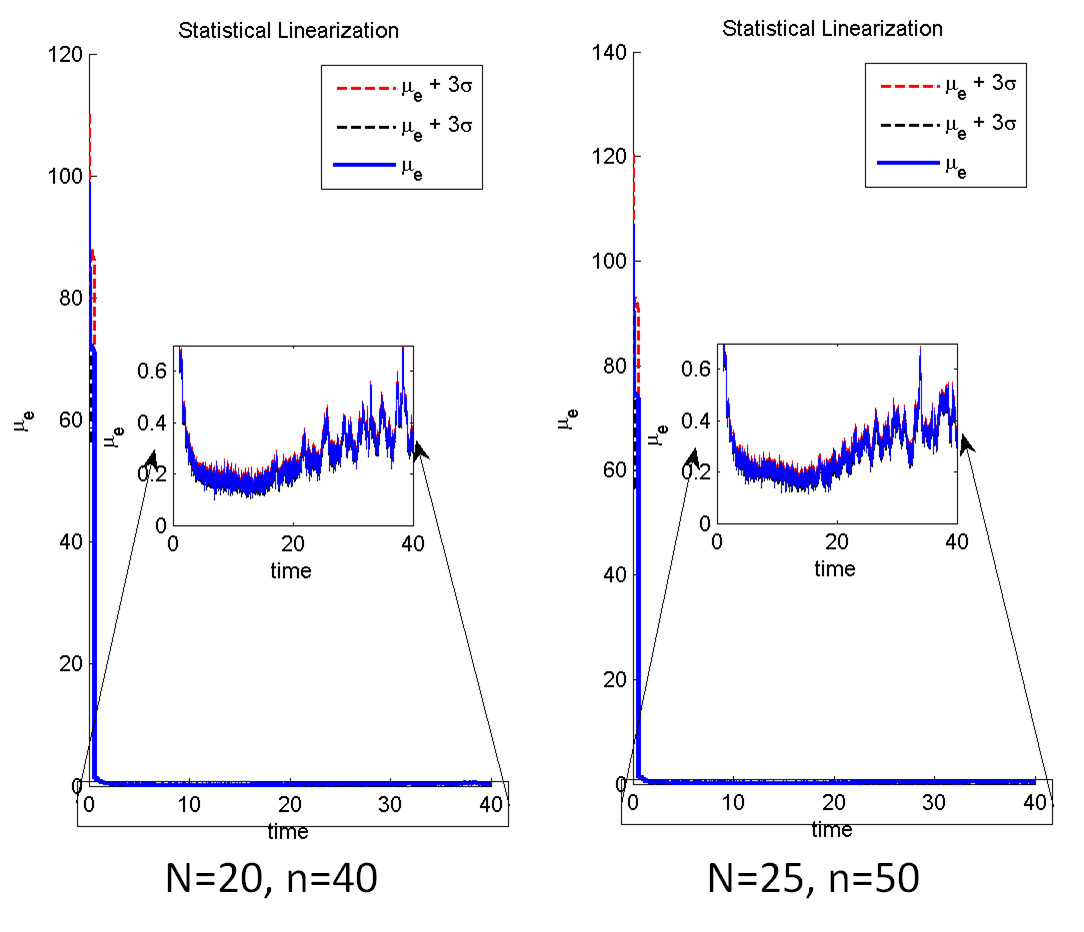
\includegraphics[width=0.8\textwidth]{figures/FIG_14}
\caption{Comparison of Original System propagation with that obtained from the two clustered model for Weakly coupled Van der Pol Oscillators after filtering}
\label{vanderpolhdcoup_clust_filter}
\end{center}
\end{figure}

From Figure~\ref{vanderpolhdcoup_clust_filter} it can be observed that the error in filtering is initially huge, and then the model approximates itself to the actual trajectory, and the error gets minimized. The average error in approximation given by $\bar{\mu}_e = \frac{1}{T}\mu_e$ has been tabulated. The time from start till the first observation is taking place is neglected for error computation. Table~\ref{vanderpolhdfilter} shows the tabulated error for some of the test cases. 

\begin{table}[H]
\scriptsize{
\begin{center}
\caption{Error in Filtering for Weakly Coupled Van der Pol Oscillators}
\label{vanderpolhdfilter}
\begin{tabular}{|c|c|}
\hline
$n$ & Statistical Linearization  \\ \hline
10    & 0.1002 \\ \hline
    20    & 0.1370 \\ \hline
    30    & 0.1998 \\ \hline
    40    & 0.2861 \\ \hline
    50    & 0.2994 \\ \hline
\end{tabular}
\end{center}
} 
\end{table}

\section{Summary}

The key contribution in the first work is the detailed study as to what extent a linearization and clustering algorithm is applicable to problem of UQ in weakly coupled dynamical system. The aim of this work is to find out the suitability of the application of the linearization and clustering algorithm to facilitate the technique of parallel computation. The usefulness of both \textit{time-domain} and \textit{space-domain} linearization has been shown through several numerical simulations on chaotic systems. With different combinations of dimension and coupling strength, the experiments are designed to increase the complexity of the test problem, posing a tough challenge for the linearization and clustering algorithm to detect the WCSs. The detailed analysis and the statistical test gives us an insight into the accuracy of the overall framework. The current method relies on linearizing the system at periodic time instances and hence the cluster structure is updated at regular intervals. Hence, such method can also be applicable to deterministic dynamical system, where the linearizing can take place with respect to the solution to the system of ODE at each time instance. It is to be noted that due to periodic updating of cluster, the identification of the cluster structure at each time instance is very important. Due to the chaotic nature of the test problems, wrong cluster structure identification at any time instance results in very high propagation of error for the future time. The ensemble of the subsystems provide an \textit{approximate} estimation instead of the \textit{exact} estimation for fast design and performance check. The test of hypothesis shows that the method of linearization and clustering works equally well, which also helps us to prove the claim of ergodicity made in Section~\ref{stat_lin_section}.

Going forward we have identified the Statistical Linearization as the preferred method of linearization due its ease in implementation and accuracy of approximation. The technique requires a one-time generation of realizations from the initial probability space. It is slower than Jacobian-based Linearization but proves to be faster and more effective than other time-domain techniques. 

The dependency of the method on the clustering technique gives scope of further research into incorporating new clustering methods into the framework. SC is easy to implement but computationally expensive for high dimensional systems. B-NMF is fast but the accuracy is often not guaranteed. The task of finding suitable clustering technique can be a never ending research given that new methods are developed every day. Furthermore, both the methods yield overlapping cluster information that can be normalized to obtain non-overlapping cluster structure. The question remains is how to efficiently utilize this overlapping cluster structure for the purpose of efficient UQ. This question is addressed in the next chapter.
\chapter{Identification of Strongly Connected Subsystems (SCSs) for Effective UQ}
\label{chap:scs}

\section{Proposed Framework for Identification of SCSs}
\label{scs_framework}

In this section, the main components of our proposed framework for SCS identification are outlined. The fundamental idea is to show how a large dimensional dynamical system can be decomposed into small interconnected subsystems (Figure~\ref{clusters_2}) to be solved in parallel. Figure~\ref{framework_fig} depicts the computational pipeline of the underlying methodology. Similar to WCS identification methodology~\cite{mukherjee2015laplacian,mukherjeecomparison} developed in Chapter~\ref{chap:wcs}, a graph-theoretic representation is adopted for a given dynamical system with involved uncertainty. Unlike the WCS identification approach, the graph is hypothesized to comprise of both weak and strong edges or couplings. The statistical linearization method is used to linearize the dynamical system in the domain of interest represented by the initial state density function (Figure~\ref{framework_fig}a). Next, a suitable overlapping community detection algorithm is applied to detect the SCSs (Figure~\ref{framework_fig}b). These SCSs determine the assignment of each node or variable to a cluster and their participation (Figure~\ref{framework_fig}c). The stochastic dynamical system corresponding to each SCS of reduced order is then propagated by a UQ method (Figure~\ref{framework_fig}d). An element-to-element product based step is applied to estimate the statistical properties of the state vector from the properties of the SCSs. These steps are followed to approximate the statistical properties, that is being propagated through the dynamics of the overall system. The overall procedure is continued till a measurement data is available. The measurement is used to filter out noise from the state variable, and the statistical properties are recalibrated using a Filtering technique (Figure~\ref{framework_fig}e). The cluster structure or the SCSs is/are then recomputed based on the updated statistical properties. The whole process continues during the required time of analysis. In the subsequent subsections, the theoretical and algorithmic details of each of these steps are discussed. 

\begin{figure}[H]
\centering
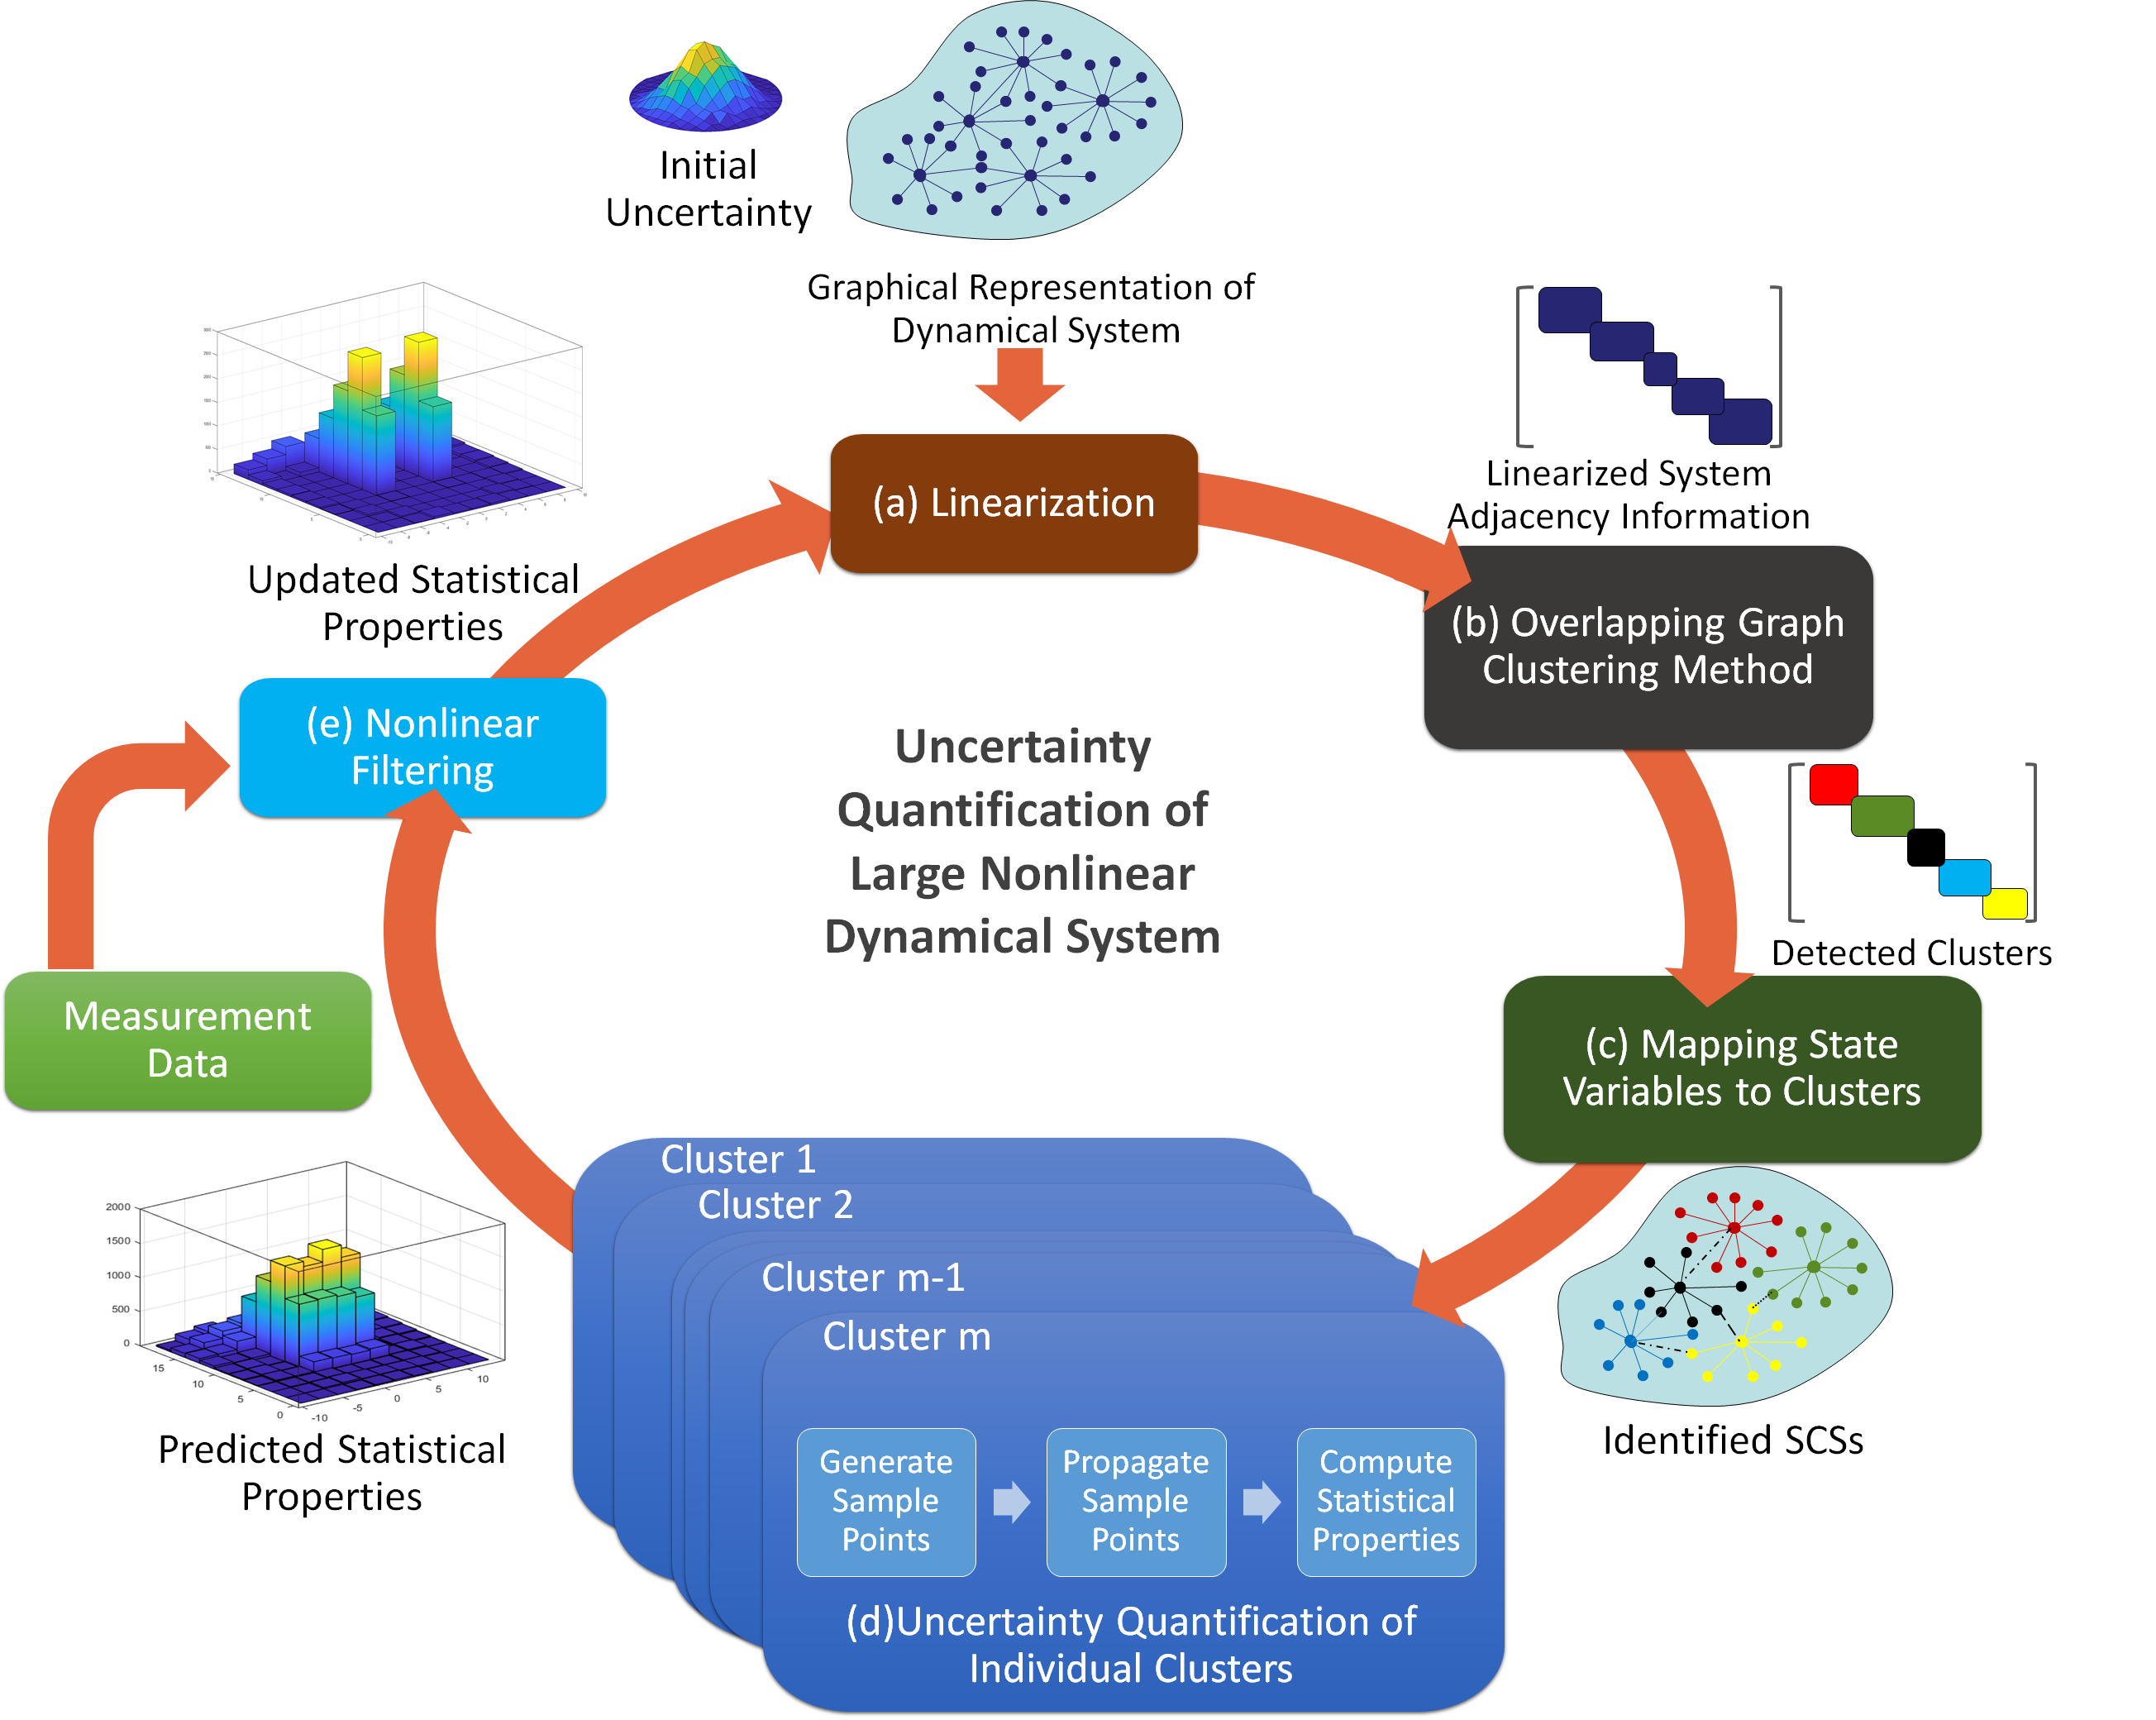
\includegraphics[scale=0.2]{figures_2/framework}
\caption{Overall Framework of the methodology}
\label{framework_fig}
\end{figure}

\section{Strongly Coupled Subsystems}

\newcommand{\bigCI}{\mathrel{\text{\scalebox{1.07}{$\perp\mkern-10mu\perp$}}}}
\newcommand{\nbigCI}{\centernot{\bigCI}}

\newcommand{\CI}{\mathrel{\perp\mspace{-10mu}\perp}}
\newcommand{\nCI}{\centernot{\CI}}

To define Strongly Connected Subsystem(SCS), a new state-space decomposition scheme is proposed with the following assumptions
\begin{itemize}
\item A state $x_i$, $i = 1$ to $n$, can participate in more than one cluster.
\item For each state, we quantify its association with a cluster. Instead of a binary $0-1$ association, we propose for a fuzzy association between 0 and 1. Such scheme can incorporate both decoupled and overlapping clusters.
%\item The association of a state with a cluster is also random.
\item The number of clusters is determined from the initial condition uncertainty and the associated dynamics for every run.
\end{itemize}

The association of the state $\textbf{x}$ in a particular cluster $j$ is defined by the variable $\textbf{z}_{j} \in \mathbb{R}^n$, $\textbf{z}_j = \lbrace z_{1j}, z_{2j},\ldots, z_{nj} \rbrace$, where $z_{ij}$, $i= 1$ to $n$ denotes the association of the state $x_i$ in cluster $j$. The variable $\textbf{z}$ has the following properties
\begin{itemize}
\item $\forall$ $i =1$ to $n$ and $j = 1$ to $m$, $0 \leq z_{ij} \leq 1$
\item $\sum_{j=1}^m z_{ij} = 1$
\end{itemize}

At each time instance, the state variable $\textbf{x}_t$ is represented in each cluster by the variable $\textbf{x}_t|j$ based on its association in a cluster $j$. A state $x_i$ having either 0, 1 (full) or partial association with a cluster. Thus, $x_i$ is represented by a linear combination of $x_{i}|j$'s, and its association $z_{ij}$, $j = 1$ to $m$ is given as,

\begin{equation}
\label{individual}
x_i = \sum_{j=1}^m  z_{ij} x_{i}|j
\end{equation}

\noindent In the vector notation the state vector is given as,

\begin{equation}
\label{main_frame}
\textbf{x}_t = \sum_{j=1}^m \textbf{z}_j \odot  \textbf{x}_t|j 
\end{equation} 

\noindent where, $\odot$ represents the element-to-element or Hadamard product and $\textbf{x}_t|j, \textbf{z}_j \in \mathbb{R}^{n}$ are $n$-dimensional random vectors. Also, for any two cluster $j_1$, $j_2 = 1$ to $m$, $j_1 \neq j_2$, we assume $\textbf{x}_t|j_1$ $\CI$ $\textbf{x}_t|j_2$. SCS or Strongly Connected Subsystem is therefore defined as the subset of $\textbf{x}_t|j$ for which $z_{ij} > \alpha$, where $\alpha$ is a very small threshold value. The values of $Z$ matrix ($Z = \lbrace z_{ij} \rbrace$) can be tabulated as shown in Table~\ref{zmatrix}.

\begin{table}[H]
\centering
\caption{The association values $z_{ij}$ tabulated in the matrix form}
\begin{tabular}{c|c|c|c|c}
\hline 
\backslashbox{States}{Clusters} & 1 & 2 & $\ldots$ & $m$ \\ 
\hline 
1 & $z_{11}$ & $z_{12}$ & \ldots & $z_{1m}$ \\  
2 & $z_{21}$ & $z_{22}$ & \ldots & $z_{2m}$ \\ 
$\vdots$ & $\ldots$ & $\ldots$ & $\vdots$ & $\ldots$ \\ 
$n$ & $z_{n1}$ & $z_{n2}$ & \ldots & $z_{nm}$ \\ 
\hline 
\end{tabular} 
\label{zmatrix}
\end{table}


The detailed theory and application of SCS for enabling UQ are discussed in subsequent subsections.


\subsection{Distribution of $\textbf{x}_t|j$}
\label{cluster_structure}

In this section, three methods for defining and estimating the statistical properties for $\textbf{x}|j$ and SCS are developed. SCS are determined as the subset $\textbf{x}_t^j|j \subset \textbf{x}|j$ for which the association in a cluster is greater than a very low threshold value. In other words $\textbf{x}_t^j|j = \lbrace x_i | z_{ij} > \alpha, i = 1 \text{ to } n \rbrace$, where $\alpha$ is the threshold parameter. In each cluster, the state variable $\textbf{x} \in \mathbb{R}^n$ into two disjoint unions $\textbf{x}_t^j|j \in \mathbb{R}^{n_j}$ and $\textbf{x}_t^{j'}|j \in \mathbb{R}^{n - n_j}$, where $\textbf{x}_t^{j}|j \cap \textbf{x}_t^{j'}|j = \emptyset $. All other association values $z_{ij}$ which are less than $\alpha$ are assumed to be 0. Under Hadamard product formulation in Equation~\ref{main_frame}, with 0 association value, the subset $\textbf{x}_t^{j'}|j$ does not contribute towards the distribution of $\textbf{x}_t$. The dynamics of the cluster $j$ evolve in the submanifold described by the reduced order subspace $\textbf{x}_t^{j}|j$ or the SCS similar to Equation~\ref{integral_wcs}. This decomposition technique facilitates the estimation of the statistical properties of SCSs and $\textbf{x}_t$ in parallel. 

 To have further ease in analysis, the concept of \textit{strong} and \textit{weak participants} have been developed. Three approximate models for $\textbf{x}_{t}^{j}|j$ have been proposed based on the participation of the subset $\textbf{x}_{\beta'}^{j}|j$ in clusters. Subsequently, the propagation equation and statistical properties for $\textbf{x}_{t}^{j}|j$ have been formulated under these approximations.
 
\subsubsection{Type I: Use of Hadamard Product}


In this approach, an SCS is defined as the set of variables  $\textbf{x}_t^j|j \in \mathbb{R}^{n_j}$ with $z_{ij} > \alpha $. By this definition, SCS has the following properties 
\begin{enumerate}
\item The state variable $\textbf{x}_t$ is a countable union of the SCSs. Thus $\bigcup _{j=1}^m \textbf{x}_t^j = \textbf{x}_t $
\item The intersection of two subsets is termed as the set of \textit{overlapping variables}. This set might not be an empty set.
\item The subsets are assumed to evolve under decoupled propagation equation and are statistically independent. Hence $\textbf{x}_t^{j_1} \CI \textbf{x}_t^{j_2}$ $\forall$ $j_1, j_1 = 1$ to $m$, $j_1 \neq _2$.   
\end{enumerate}
In each cluster, the submanifold $\textbf{x}_t^j$ for the SCS is defined by the following SDE,

\begin{equation}
\dot{\textbf{x}_t^j} = f_j(\textbf{x}_t^j)  
\end{equation}  

Thus, $m$ reduced order subsystems of order $n_j << n$ are solved instead of solving Equation~\ref{integral_whole}. Under this framework, the overlapping variables evolve with different propagation equation in different clusters. Finally, the approximate solution to Equation~\ref{moment_whole} and other statistical properties of $\textbf{x}_t$ are computed using the results from different clusters through the Hadamard product formulation (outlined in Section~\ref{hadamard_statistics}). The process of mapping state variables to overlapping clusters is shown in Figure~\ref{framework_TypeI}. 

\begin{figure}[H]
\begin{center}
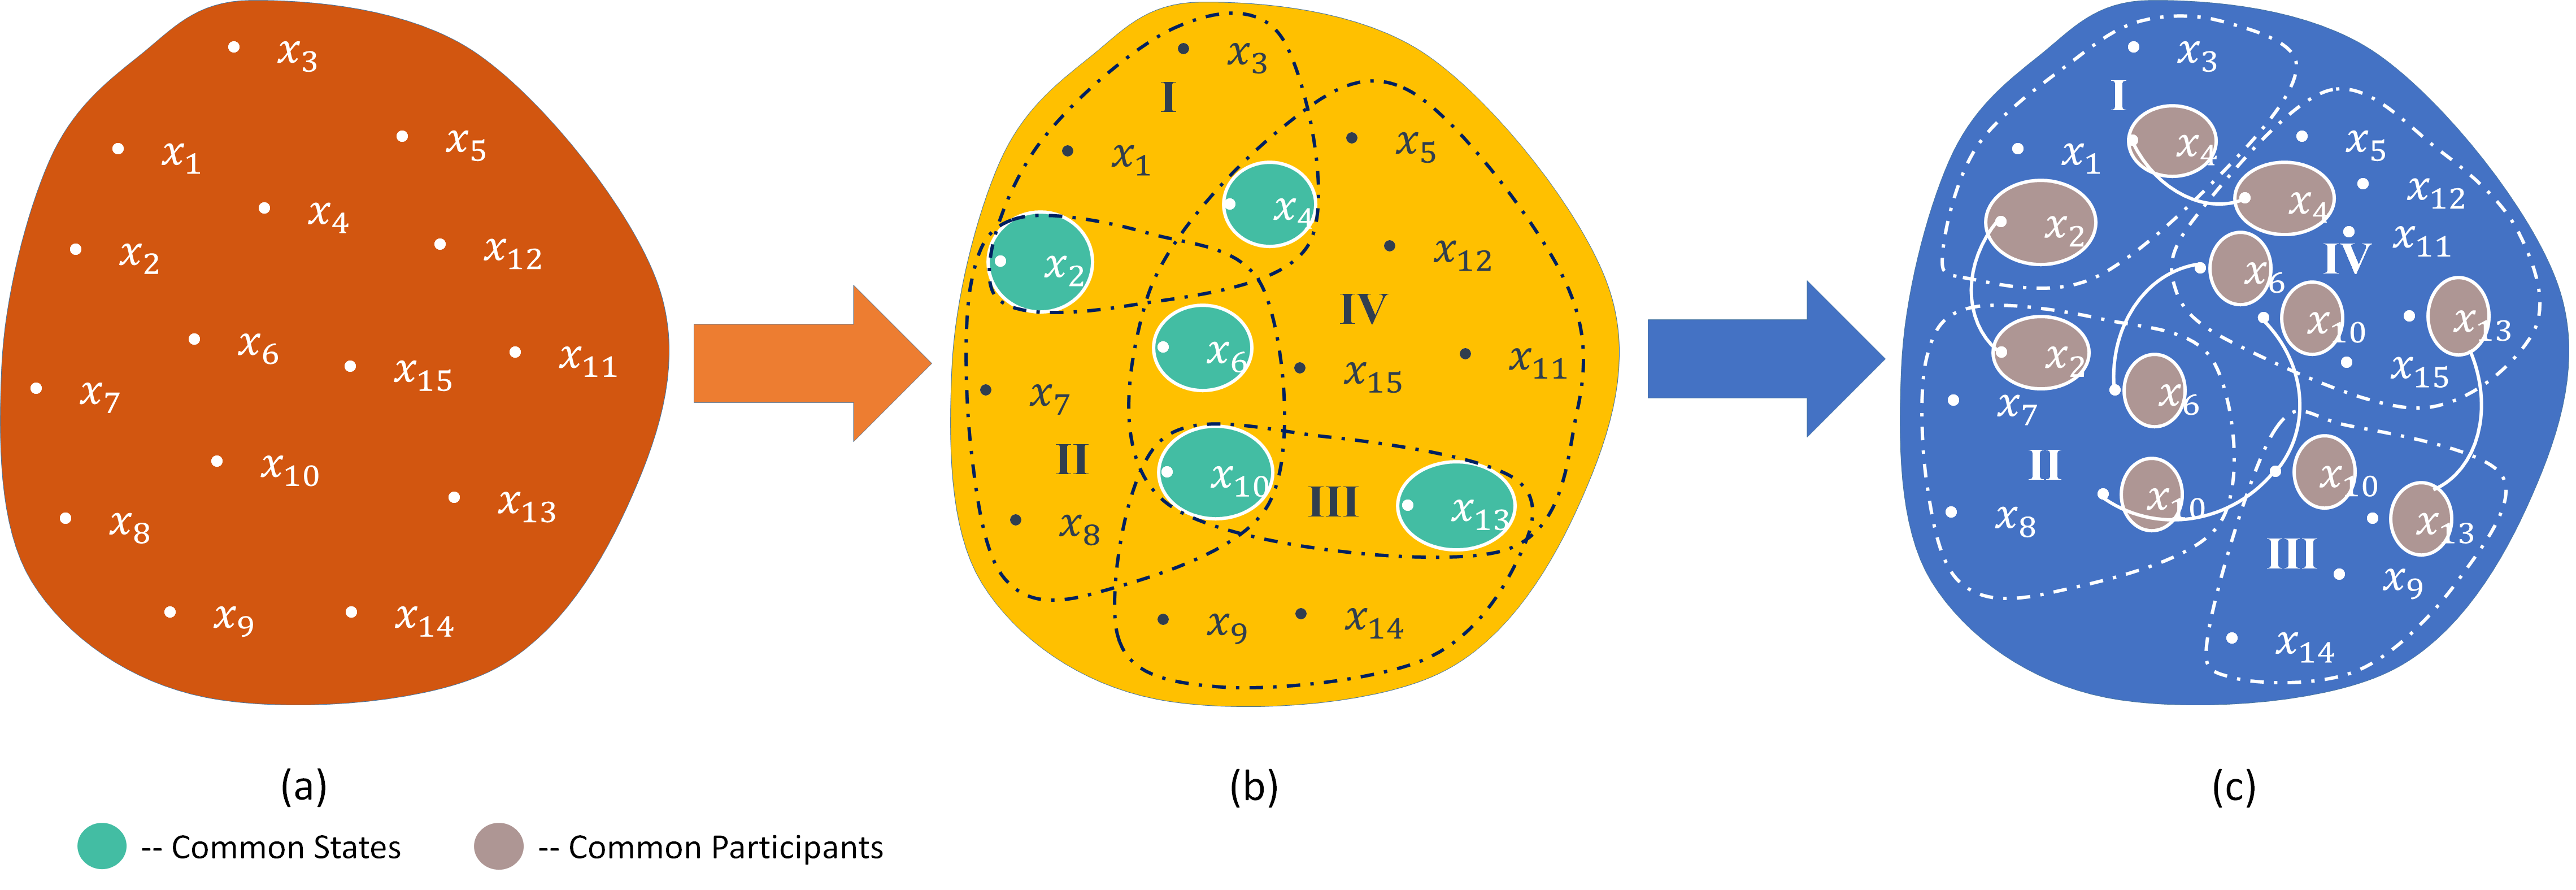
\includegraphics[width=\textwidth]{figures_2/TypeI}
\caption{Overall Framework of the Type I method of clustering: (a) Overall state-space domain (b) Identification of overlapping clusters (common states encircled) and (c) States being mapped to non-overlapping clusters with common states participating in more than one cluster with same initial condition.}
\label{framework_TypeI}
\end{center}
\end{figure}


\subsubsection{Type II: Identification of strong and weak participants}
\label{type_II}

In this approach, we assume a higher threshold value $\beta$, with $\beta > \alpha$. This decides the level of participation of $\textbf{x}_t^{j}|j$ in the cluster $j$. We further break the subset $\textbf{x}_j|j$ into two unions $\textbf{x}_{\beta}^{j}|j \in \mathbb{R}^{n_{j_\beta}}$ and $\textbf{x}_{\beta'}^{j}|j \in \mathbb{R}^{n_j - n_{j_\beta}}$, with $\textbf{x}_{\beta}^{j}|j \cap \textbf{x}_{\beta'}^{j}|j = \emptyset$. The subset $\textbf{x}_{\beta}^{j}|j = \lbrace x_i | z_{ij} > \beta, i = 1 \text{ to } n_j \rbrace$ is labeled as the set of \textit{strong participants} and the other subset $\textbf{x}_{\beta'}^{j}|j$ as the set of \textit{weak participants}. We assume the initial distribution for $\textbf{x}_j^{\beta'}|j$ and the subset is provided to the propagation equation for $\textbf{x}_j^{\beta'}|j$ as an input variable. While the properties of $\textbf{x}^j_t$ remain the same as that in Type I, the properties of the subsets $\textbf{x}_{\beta}^{j}|j$'s are different:
\begin{enumerate}
\item The union of the subsets $\textbf{x}_{\beta}^{j}|j$'s may not be equal to $\textbf{x}_t$.
\item The intersection of two subsets $\textbf{x}_{\beta}^{j}|j$'s is termed as the set of \textit{overlapping variables}. This set might not be an empty set. The overlapping variables are propagated in the same way as in Type I.
\item The subsets are assumed to evolve under decoupled propagation equation and are statistically independent. Hence $\textbf{x}_{\beta}^{j_1}|j_1 \CI \textbf{x}_{\beta}^{j_2}|j_2$ $\forall$ $j_1, j_1 = 1$ to $m$, $j_1 \neq _2$. 
\end{enumerate}
 The propagation equation for $\textbf{x}_{\beta}^{j}|j$ is thus:

\begin{equation}
d \textbf{x}_{\beta}^{j}|j = f_{j_\beta} (\textbf{x}_{\beta}^{j}|j, \textbf{x}_j^{\beta'}|j)dt 
\end{equation}

This is a reduced order system of order $n_{j_\beta} \leq n_j$. For the purpose of calculating the final mean and covariance, a modified association matrix $Z^s$ is constructed using the following steps:

\begin{enumerate}
\item Initialize $Z^s$ to $Z$. 
\item The associations of the weak participants are assumed to be 0 as $z^s_{ij} = 0 $ $\forall$ $z_{ij} < \beta$.
\item Each row $i$ of $Z^s$ is further normalized as $z_{ij}^s = z_{ij}^s/ \sum_{j = 1}^m z_{ij}^s$.
\end{enumerate}

Similar to Type I, the statistical properties of $\textbf{x}_t$ are computed using the results from different clusters and the modified association matrix derived from the Hadamard product formulation (outlined in Section~\ref{hadamard_statistics}). The process of mapping state variables to overlapping clusters is shown in Figure~\ref{framework_TypeII}. 

\begin{figure}[H]
\begin{center}
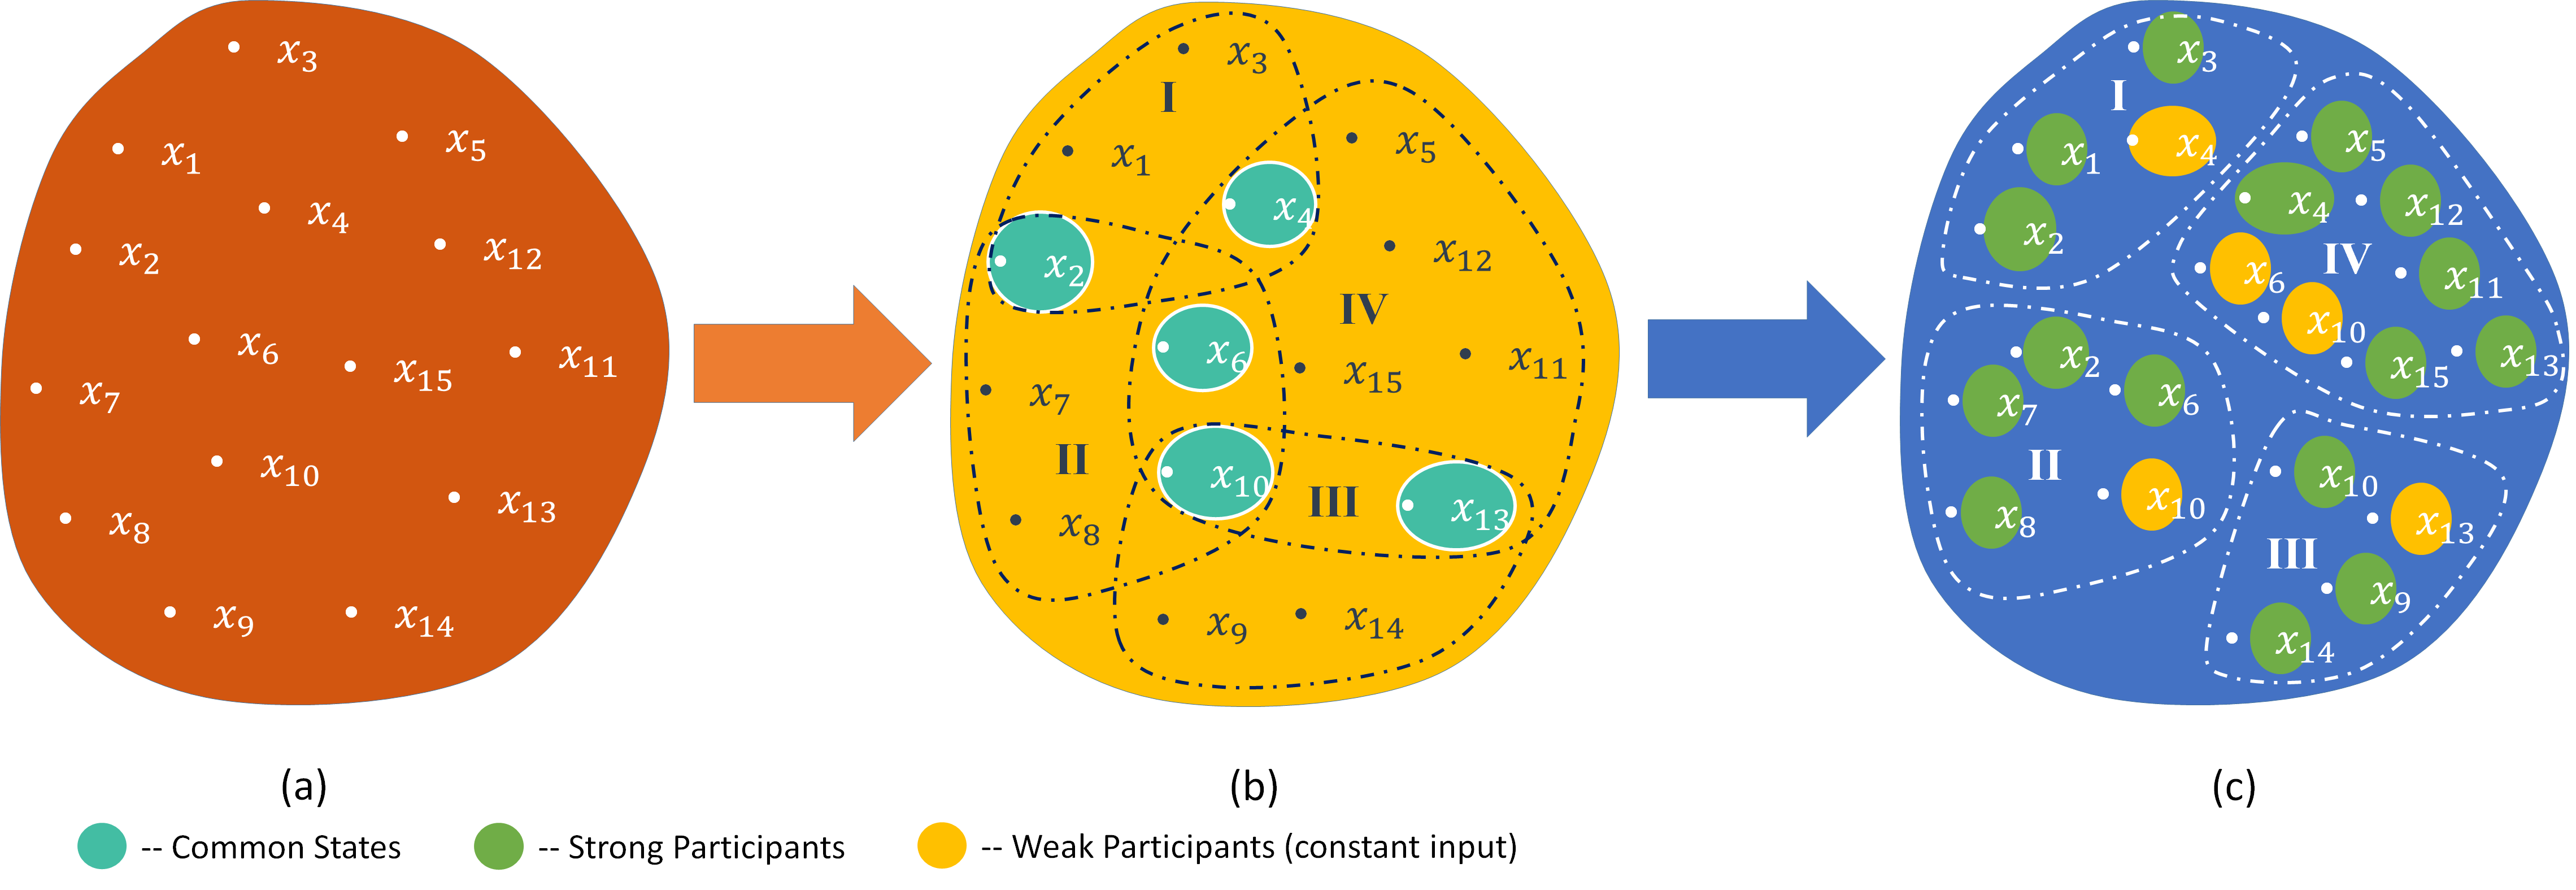
\includegraphics[width=\textwidth]{figures_2/TypeII}
\caption{Overall Framework of the Type II method of clustering: (a) Overall state-space domain (b) Identification of overlapping clusters (common states encircled) and (c) Identification of \textit{Strong} and \textit{Weak Participants}. \textit{Weak Participants} acting as constant input.}
\label{framework_TypeII}
\end{center}
\end{figure}

\subsubsection{Type III: Identifying Decoupled Subsystems}

This methodology is analytically similar to the method of identifying WCSs. A binary association matrix $Z^{decoup} \in \mathbb{R}^{n \times m}$ is constructed from the original matrix $Z$. In a row $i = 1$ to $n$ the maximum value of $z_{ij}$  is found out and is set to 1. The rest of the values are set to 0. This procedure gives us the $Z^{decoup}$ matrix. Thus, a state can participate in only one cluster and there is no overlap. The set $\textbf{x}^d_j|j \in \mathbb{R}^{n_d}$ contains only the states for which $z_{ij'}^{decoup} = 1$. Thus,
\begin{enumerate}
\item The subsets are disjoint partitions of $\textbf{x}_t$. This means $\bigcup _{j=1}^m \textbf{x}^d_j|j =\textbf{x}_t$ and $\textbf{x}^d_{j_1}|j_1 \CI \textbf{x}^d_{j_2}|j_1 = \emptyset$ $\forall$ $j_1, j_1 = 1$ to $m$, $j_1 \neq _2$. 
\item The subsets are decoupled and statistically independent. 
\end{enumerate}
Based on these assumptions, the submanifold $\textbf{x}_j^{d}|j$ is defined by the following SDE:

\begin{equation}
\dot{\textbf{x}}_j^{d}|j = f_j({\textbf{x}}_j^{d}|j)    \hspace{5 mm}  \textbf{x}_0 = {\textbf{x}}_j^{d}|j 
\end{equation}

The process of mapping state variables to overlapping clusters is shown in Figure~\ref{framework_TypeIII}. This is a reduced order system of order $n_d \leq n_{j_\beta} \leq n_j$. The next subsection discusses the numerical method for computing the association matrix $Z$ for the system defined in Equation~\ref{stochdyn}. 


\begin{figure}[H]
\begin{center}
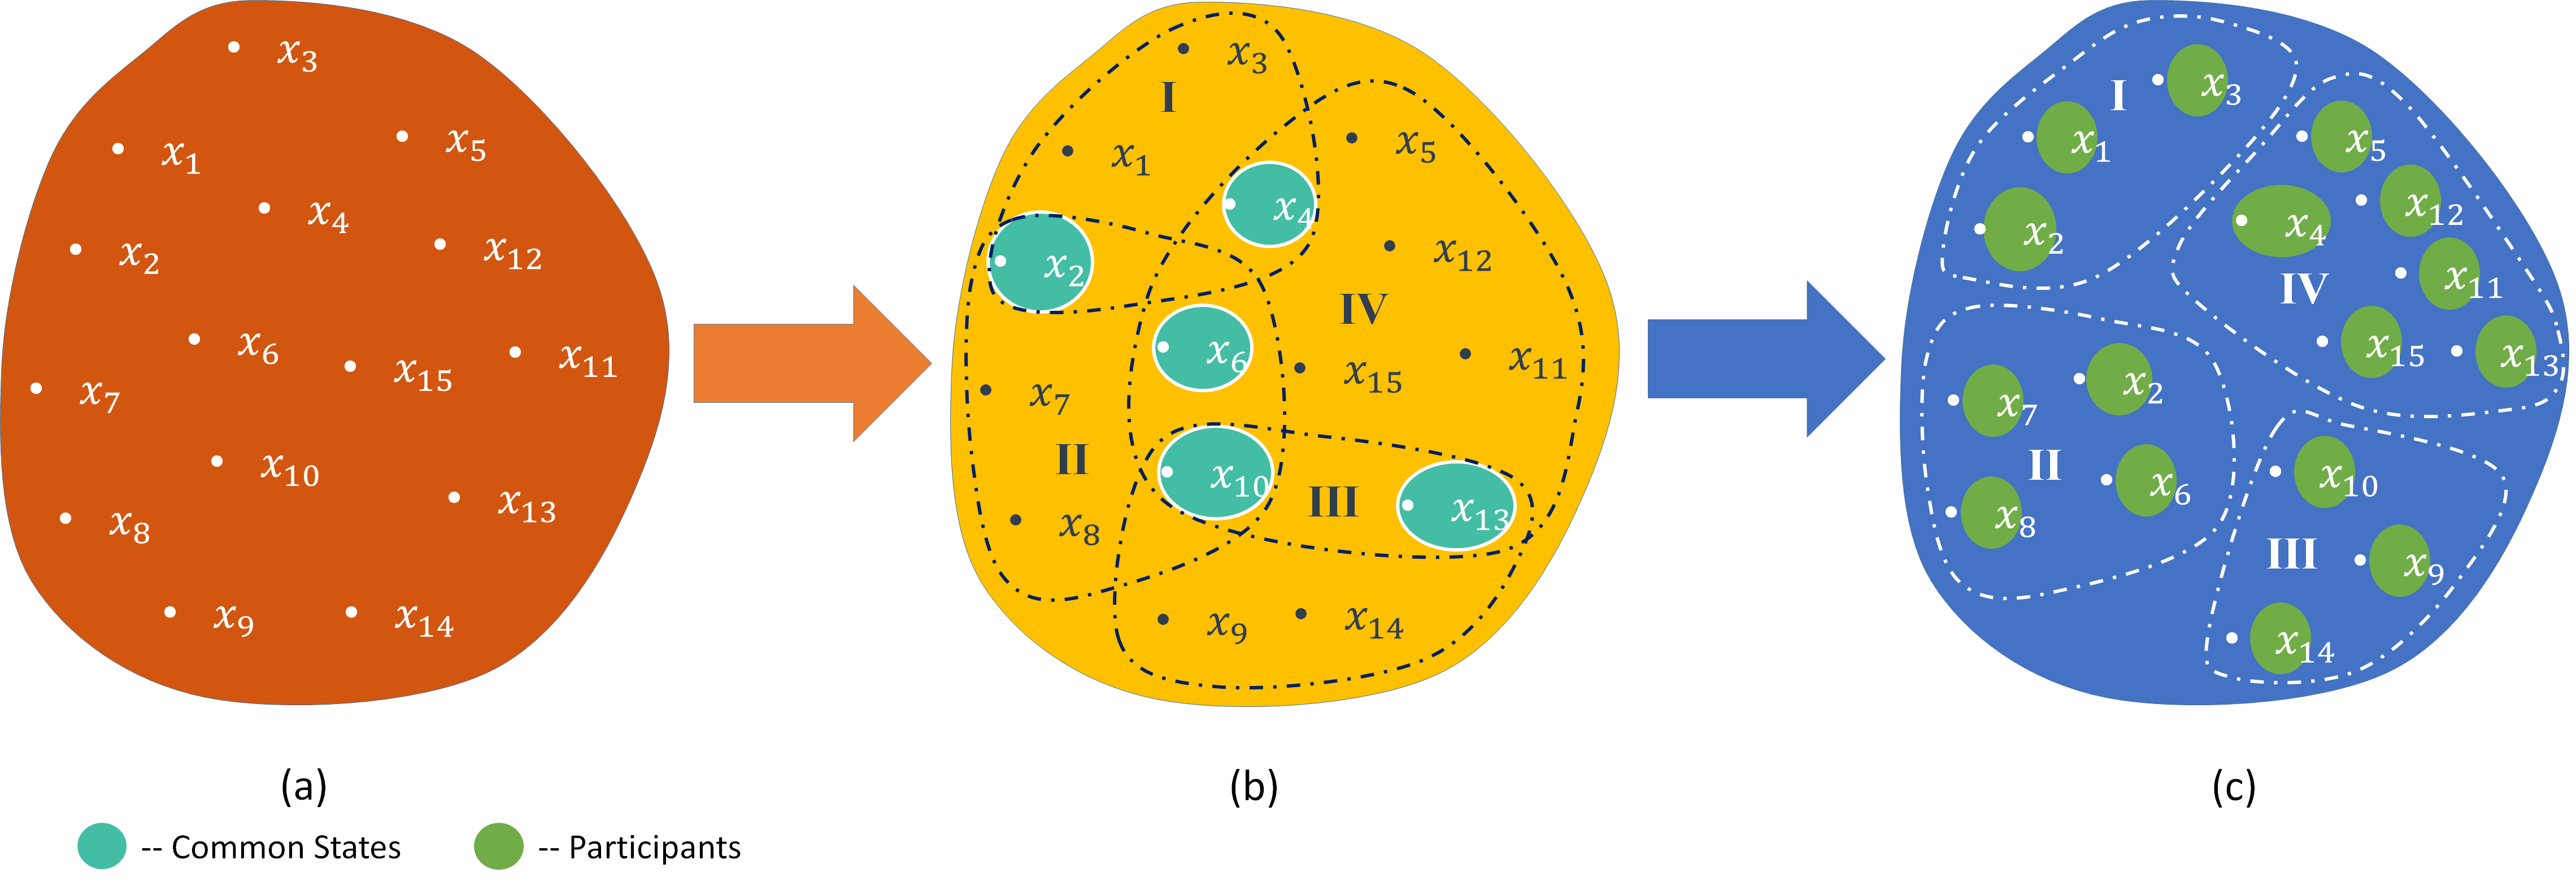
\includegraphics[width=\textwidth]{figures_2/TypeIII}
\caption{Overall Framework of the Type III method of clustering: (a) Overall state-space domain (b) Identification of overlapping clusters (common states encircled) and (c) Identification of non-overlapping clusters}
\label{framework_TypeIII}
\end{center}
\end{figure}


\section{Overlapping Graph Clustering}

The study of overlapping community has been a recent addition to the world of scientific research. Instead of detecting disjoint community in a network, in overlapping community framework, a node in a network can participate in multiple communities. In this context, Baumes \textit{et al.}~\cite{baumes2005finding} proposed a two-step algorithm to identify disjoint clusters, followed by an iterative method of assigning nodes to clusters till a density function is improved. Palla \textit{et al.} have developed a clique-based method and have applied the method to protein network comprising of 30,739 links~\cite{palla2005uncovering}. Algorithms such as LFM~\cite{lancichinetti2009detecting}, MONC~\cite{havemann2011identification}, CPMw~\cite{farkas2007weighted}, SCP~\cite{kumpula2008sequential} have extended the earlier work to enhance the applicability of community detection algorithms. OSLOM\cite{lancichinetti2011finding} and several effective overlapping community detection algorithms identifying overlapping cluster structures in complex networks also exist~\cite{shen2009detect,cazabet2010detection,padrol2010overlapping}. Although all the works mentioned above detect overlapping clusters, they do not quantify the degree of participation of a node in a given cluster. Fuzzy based clustering methods have been developed to address the shortcoming of quantifying the degree of participation. The \textit{fuzzy k-means} algorithm instead of optimizing the sum of the Euclidean distance between the nodes and the cluster centers, uses a weighted objective function is used to quantify the degree of participation~\cite{dunn1974well}. Zhang \textit{et al.}~\cite{zhang2007identification} has combined the fuzzy k-means clustering algorithm with the well-established method of Spectral Clustering~\cite{von2007tutorial}. Distribution based algorithms have been further developed, whereby the association of a node to a cluster is modeled as a probability distribution and is updated with the availability of the adjacency information~\cite{magdon2011ssde,latouche2011overlapping,psorakis2011overlapping}. In our current work, the Non-negative matrix factorization based algorithm to detect the degree of association of a node to a cluster~\cite{psorakis2011overlapping} have been used. This algorithm iteratively minimizes the rank of the degree matrix along with finding the association of the nodes in each cluster.


\section{Hadamard Product and Multivariate Statistics}
\label{hadamard_statistics}

%Let us explore the statistical properties of the variable $\textbf{x}_t$. First, we formulate the moments for an individual state variable $x_i$. As explained earlier, the state variable can be decomposed into independent clusters with degrees of association as given in Equation~\ref{individual} and \ref{main_frame}.   

Once the statistical properties of the SCSs are determined from the propagation and moment equations as given in Section~\ref{cluster_structure}, the first and second order moments for a state variable $x_i$  under the formulation of Equation~\ref{individual} is given as:

\begin{equation}
E \left[x_i \right] = E \left[ \sum_{j=1}^m z_{ij} x_{i}|j \right] =\sum_{j=1}^m  z_{ij} E \left[  x_{i}|j  \right]  
\end{equation}

and,

\begin{equation}
E \left[x_i^2 \right] = E \left[ \left( \sum_{j=1}^m z_{ij} x_{i}|j  \right)^2 \right] =\sum_{j=1}^m  z_{ij}^2 E \left[  x^2_{i}|j  \right]  + \sum_{j=1}^{m-1} \sum_{k=j+1}^m z_{ij}z_{ik}  E \left[  x_{i}|j  \right] E \left[  x_{i}|k  \right]
\end{equation}

Thus, the covariance formulation is given as: 

\begin{equation}
\mathbf{var}(x_i) = \sum_{j=1}^m z^2_{ij} \mathbf{var} (x_{i})
\end{equation}



\noindent Similarly, a general expression for any $\alpha^{\text{th}}$ order moment can be written using multinomial expansion as:

\begin{equation}
\begin{array}{ll}
E \left[x_i^{\alpha} \right] = \displaystyle E \left[ \left( \sum_{j=1}^m z_{ij} x_{i}|j  \right)^{\alpha} \right] &= \displaystyle E \left[ \sum_{k_1 + k_2 + \ldots + k_m = \alpha} \begin{pmatrix}
\alpha \\ k_1,k_2,\ldots,k_m
\end{pmatrix}  \prod_{1 \leq j \leq m} x^{k_j}_{i}|j  \; z^{k_j}_{ij} \right] \\
&= \displaystyle  \sum_{k_1 + k_2 + \ldots + k_m = \alpha} \begin{pmatrix}
\alpha \\ k_1,k_2,\ldots,k_m
\end{pmatrix}  \prod_{1 \leq j \leq m} z^{k_j}_{ij} \prod_{1 \leq j \leq m} E \left[ x^{k_j}_{i}|j \right]
\end{array}
\end{equation}

For the state vector $\textbf{x}_t$, the moment equations for the first two order under the formulation of Equation~\ref{main_frame} are given as:

\begin{equation}
\label{mean}
E \left[\textbf{x}_t \right] = E \left[ \sum_{j=1}^m \textbf{z}_j \odot \textbf{x}_t|j  \right] =\sum_{j=1}^m  \textbf{z}_j \odot E \left[  \textbf{x}_t|j  \right]  
\end{equation}

and,

\begin{equation}
\begin{array}{ll}
E \left[\textbf{x}_t \textbf{x}^T_t  \right] &= \displaystyle  \sum_{j=1}^m E \left[\left( \textbf{z}_j \odot \textbf{x}_t|j\right) \left( \textbf{z}_j \odot \textbf{x}_t|j\right)^T \right] + \sum_{j=1}^{m-1} \sum_{k=j+1}^m E \left[\left( \textbf{z}_j \odot \textbf{x}_t|j\right) \left( \textbf{z}_k \odot \textbf{x}_t|k\right)^T \right] \\
&= \displaystyle \sum_{j=1}^m \left( \textbf{z}_j \textbf{z}^T_j  \right) \odot E \left[ {\textbf{x}_t|j} \; {\textbf{x}_t|j}^T \right] + \sum_{j=1}^{m-1} \sum_{k=j+1}^m \left( \textbf{z}_j \textbf{z}^T_k  \right) \odot E \left[ {\textbf{x}_t|j}\right] E \left[{\textbf{x}_t|k} \right]^T
\end{array}
\end{equation}

Thus, the covariance matrix is given as:

\begin{equation}
\label{covariance}
\mathbf{cov}(\textbf{x}_t) = \sum_{j=1}^m \left(\textbf{z}_j \textbf{z}^T_j \right) \odot \mathbf{cov} \left( \textbf{x}_t|j \right)
\end{equation}

Furthermore, the moment generating function (mgf) for $x_i$ can be written as:

\begin{equation}
\begin{array}{ll}
M_{x_i}(\tau) &=  E \left[ e^{\tau x_i} \right] = E \left[ e^{\tau \sum_{j=1}^m  z_{ij} x_{i}|j} \right] = \displaystyle \prod_{j=1}^m E \left[e^{\tau (z_{ij} x_{i}|j )}  \right] \\
&= \displaystyle \prod_{j=1}^m M_{x_{i}|j} (z_{ij} \tau)
\end{array}
\end{equation}

Hence, the mgf of $\textbf{x}_t$ is given as:


\begin{equation}
\begin{array}{ll}
M_{\textbf{x}_t}(\bm{\tau}) &=  E \left[ e^{\bm{\tau}^T \textbf{x}_t} \right] =  E \left[ e^{\bm{\tau}^T \sum_{j=1}^m  \textbf{z}_j \odot \textbf{x}_t|j }  \right] = \displaystyle \prod_{j=1}^m E \left[e^{(\textbf{z}_j \odot \bm{\tau} )^T \textbf{x}_{t}|j }  \right] \\
&= \displaystyle \prod_{j=1}^m M_{\textbf{x}_t|j} (\textbf{z}_j \odot \bm{\tau})
\end{array}
\end{equation}

Equation~\ref{mean} and~\ref{covariance} have been used to estimate the statistical properties of the state variable $\textbf{x}$ obtained from the solution to Equation~\ref{integral_whole}. 

\section{Kalman Filter and Updating of Cluster Structure}
\label{ukf_clust}
In this section, the different subroutines are grouped to describe the overall framework. The linearization and clustering method described in Section~\ref{cluster_structure} is coupled with standard UQ method of Unscented Kalman Filter (UKF)~\cite{julier1997new} to analyze a high dimensional system defined in Chapter~\ref{chap:uq}. UKF has been the preferred method of UQ owing its speed and accuracy in estimating moments up to the second order of a Gaussian random vector by generating fewer sample points. 

% UKF proposes the following deterministic formulation for generating \textit{Sigma Points} from a Gaussian random variable $\textbf{x} \sim \mathcal{N}(\mu,\Sigma), \textbf{x} \in \mathbb{R}^n$,
% \begin{equation}
% \label{sigmapt}
% \begin{array}{lr}
% \mathcal{X}_0 = \mathbf{\mu} &W_0 = \kappa /(n+ \kappa)  \\
% \mathcal{X}_i = \mathbf{\mu} + \left( \sqrt{(n+ \kappa) \Sigma} \right)_i  &W_i = 1 /2(n+ \kappa)  \\
% \mathcal{X}_{i+n} = \mathbf{\mu} - \left( \sqrt{(n+ \kappa) \Sigma} \right)_i  &W_{i+n} = 1 /2(n+ \kappa)
% \end{array}
% \end{equation}
% \noindent $\left( \sqrt{(n+ \kappa) \Sigma} \right)_i$ is the $i$th row or column of the matrix square root of $(n+ \kappa) \Sigma$. These points accurately estimate the moment of $\textbf{x}$ up to the second order. These moment equations are given as,
% \begin{equation}
% \label{prop}
% \begin{array}{l}
% {\mu} =  \displaystyle \sum_{i=1}^{2n+1} W_i \mathcal{X}_i   \\
% \Sigma = \displaystyle \sum_{i=1}^{2n+1} W_i (\mathcal{X}_i - {\mu})(\mathcal{X}_i - {\mu})^T  \notag
% \end{array}
% \end{equation} 

Due to the coupling between the state variables, it is assumed that the cluster structure may change with time. Subsequently, there is a requirement of changing the cluster structure after a finite time evolution of the SCSs. This time is determined by the availability of measurement data. Measurements or observations are obtained from the actual running of the system at different time intervals. The measurement data is used to periodically update the statistical properties of the state variables using the UKF. The updated mean and covariance is used as the uncertainty information required to cluster the state space for the next finite time interval till the next measurement becomes available. All the methods mentioned above are combined to analyze a given large system. The different steps involved are as given below:

\begin{enumerate}
\item Given the problem 
\begin{equation}
\label{scs_meas_eqn}
\begin{array}{lr}
\dot{\textbf{x}}_t = f(\textbf{x}_t) & \textbf{x}_{t_0} = \textbf{x}_0 \\
\textbf{z}_t = \textbf{x}_t + \nu
\end{array}
\end{equation}
Where, $\textbf{z}_t$ is the measurement at a given time, and $\nu \sim \mathcal{N}(0,R_{\textbf{z}})$ is the measurement error.

\item At a time $t_0$, the nonlinear system is linearized as, 
\begin{equation}
f(\textbf{x}_{t_k}) = A_{sl}\textbf{x}_{t_k} + b_{sl}
\end{equation}
and clustered as per methods described in Section~\ref{cluster_structure}. At the end of this step, the number of subgroups or clusters in the state variables is identified, along with the association matrix $Z$ as given in Table~\ref{zmatrix}. 

\item The state-space is decomposed into SCS from the values of the association matrix $Z$ using the three methods of mapping described in Section~\ref{cluster_structure}.

\item Sigma points are generated using Equation~\ref{sigmapt} from the reduced order SCSs. The submanifold for each SCS is propagated as described in Section~\ref{cluster_structure} up to a certain time $t_k$. The mean and covariance for each SCS are estimated using Equation~\ref{prop}.

\item Once, the UQ of all the SCSs is complete, the mean and covariance of $\textbf{x}_{t_k}$ are computed using Equation~\ref{mean} and~\ref{covariance}.

\item Step 4 and 5 are continued up to a time $t_k + h$ till a measurement $\textbf{z}_{t_k + h}$ is available. Once a measurement update is available, the mean and covariance values are updated using the following steps of the UKF

\begin{enumerate}
\item The innovation covariance is then computed as:
\begin{equation}
P_{\nu \nu} = R_{\textbf{z}} + P_{k+h|k+h-1}
\end{equation}
\item The cross correlation matrix is computed as $P_{k+h|k+h-1}$
\item The Kalman gain is computed as: 
\begin{equation}
K = P_{k+h|k+h-1} P_{\nu \nu}^{-1}
\end{equation}
\item The measurement update is carried out:
\begin{equation}
\begin{array}{l}
\mu_{k+h|k+h} = \mu_{k+h|k+h-1} + K(\textbf{z}_{t_k + h} - \mu_{k+h|k+h-1})  \\
P_{k+h|k+h} = P_{k+h|k+h-1} - K P_{\nu \nu} K^T
\end{array}
\end{equation}

\item The above-defined recalibration of mean and covariance helps in updating the cluster structure of $\textbf{x}$. Using the updated statistical properties and the velocity function $f(\cdot)$, the association matrix $Z$ is recomputed using the methods described in Section~\ref{cluster_structure}. The state variables are further mapped into clusters using the three methods of mapping (Section~\ref{cluster_structure}). Steps 2-5 are repeated, and step 6 is used when a measurement becomes available. These steps are repeated iteratively till the whole analysis is complete.
\end{enumerate}


\end{enumerate}

\section{Three Coupled Lorenz Attractors}
\label{three_osc}
\subsection{The Problem Statement}

\begin{enumerate}
\item Coupled Lorenz Oscillators~\cite{lorenz1963deterministic},
\begin{equation}
\label{2d_lorenz}
\begin{array}{l}
\dot{x}_i = \sigma_i(y_i - x_i) +\epsilon(x_{i+1} - 2x_i + x_{i+1}) \\
\dot{y}_i = x_i (\rho_i - z_i) - y_i \\
\dot{z}_i = x_i y_i - \beta_i z_i \hspace{5mm} i = 1,2,3
\end{array}
\end{equation}
\item The coupling strength is $\epsilon = 1$. Other parameters are $\sigma_i = \begin{bmatrix} 8 & 9 & 12 \end{bmatrix}$, $\rho_i = \begin{bmatrix} 30 & 31 & 35 \end{bmatrix}$ and $\beta_i = \begin{bmatrix} 2.2432 & 2.9077 & 2.5923 \end{bmatrix}$
\item The measurement equation is $h = \textbf{x} + \nu$. Measurements are available from time 0 to $T = 10$ seconds at every $1$ second interval.
\item Initial distribution as $\textbf{x} \in \mathcal{N}(\bm{\mu}_{\textbf{x}},\Sigma_{\textbf{x}})$
\item Thresholds for clustering are $\alpha = 10^{-3}$ and $\beta = 0.1$
\end{enumerate}

\subsection{Association Matrix $Z$ at $t = 0$}

\begin{itemize}
\item From the initial distribution of $\textbf{x}_0$, generate $2n+1$ sigma points. These points are used to develop the statistically linearized matrix as given in Equation~\ref{stat_lin}.
\item The association matrix $Z = \begin{bmatrix}
z_{1} & z_2 & \ldots & z_m
\end{bmatrix} \in \mathbb{R}^{n \times m}$  is obtained by applying the Bayesian NMF on the matrix $A_{sl}$.
\item Any value in the matrix $Z$ less than $\epsilon_1$ is replaced by 0. The initial $Z$ matrix (Similar to Table~\ref{zmatrix}) for the problem is given in Table~\ref{init_zmatrix}. 
\newpage
\begin{table}[H]
\caption{Initial $Z$ matrix for Problem Statement in Equation~(\ref{2d_lorenz})}
\label{init_zmatrix}
\centering
\begin{tabular}{c|c|c|c}
\hline 
\backslashbox{States}{Clusters} & 1 & 2 & 3 \\ 
\hline
1 & 0.9474 & 0.0526 & 0 \\ 
2 & 1 & 0 & 0 \\ 
3 & 1 & 0 & 0 \\ 
4 & 0.0455 & 0.9091 & 0.0455 \\ 
5 & 0 & 1 & 0 \\ 
6 & 0 & 1 & 0 \\ 
7 & 0 & 0.0370 & 0.9630 \\ 
8 & 0 & 0 & 1 \\ 
9 & 0 & 0 & 1 \\ 
\hline 
\end{tabular} 
\end{table}
\end{itemize}

\subsection{Propagation Equation for $\textbf{x}_t$ using the three different approaches}

As discussed before, under the different type of models adopted, different cluster structures from the same association matrix are obtained. For analysis of the system up to the next available measurement, the three different models for time interval $[0,1]$ at every 0.01s have been simulated. 

\subsubsection{Type I Method}

Using Type I approach, the identified clusters are tabulated in Table~\ref{Type1_cluster_lorenz}.

\begin{table}[H]
\centering
\caption{State Space cluster for Type I method}
\label{Type1_cluster_lorenz}
\begin{tabular}{c|c|c}
\hline 
Cluster & $\textbf{x}_t^j|j$ & States \\
\hline 
1 & $\textbf{x}_t^1|1$ & $\lbrace x_1,y_1,z_1,x_2 \rbrace$ \\ 
2 & $\textbf{x}_t^2|2$ & $\lbrace x_1,x_2,y_2,z_2,x_3 \rbrace$  \\ 
3 & $\textbf{x}_t^3|3$ & $\lbrace x_2, x_3, y_3, z_3 \rbrace$ \\ 
\hline 
\end{tabular} 
\end{table}

The propagation equation for each cluster involves only the states participating in the cluster. For example, the propagation equations for cluster 2 is given as follows:

\begin{equation}
\label{type1:lorenz}
\begin{array}{l}
\dot{x}_1 = -\sigma_1 x_1 +\epsilon(- 2x_1 + x_2) \\
\dot{x}_2 = \sigma_2(y_2 - x_2) +\epsilon(x_1 - 2x_2 + x_3) \\
\dot{y}_2 = x_2 (\rho_2 - z_2) - y_2 \\
\dot{z}_2 = x_2 y_2 - \beta_i z_2  \\
\dot{x}_3 = -\sigma_3 x_3 +\epsilon(x_2 - 2x_3) \\
\end{array}
\end{equation}

Equation~\ref{type1:lorenz} is a 5th order system of equation involving 5 random variables. Using UT, Equation~\ref{type1:lorenz} can be solved using $2 \times 5 + 1 = 11$ sigma points. The Mean and Covariance for $\textbf{x}_t$ are calculated using the Hadamard Product formulation (Equation~\ref{mean} and~\ref{covariance}). With the availability of measurement data, the mean and covariance are calibrated and the association matrix is updated as described in Step 6 in Section~\ref{ukf_clust}.

\subsubsection{Type II Method}
 
Using Type II approach, the identified \textit{strong and participant} subsets $\textbf{x}_{\beta}^{j}|j$ and $\textbf{x}_{\beta'}^{j}|j$ from the association matrix are listed in Table~\ref{Type2_cluster_lorenz},

\begin{table}[H]
\centering
\caption{State Space cluster for Type II method}
\label{Type2_cluster_lorenz}
\begin{tabular}{c|c|c|c|c}
\hline 
Cluster & $\textbf{x}_{\beta}^{j}|j$ & States & $\textbf{x}_{\beta'}^{j}|j$ & States \\ 
\hline
1 & $\textbf{x}_{0.1}^{1}|1$ & $\lbrace x_1,y_1,z_1 \rbrace$ & $\textbf{x}_{0.1'}^{1}|1$ & $ \lbrace x_2 \rbrace$ \\ 
2 & $\textbf{x}_{0.1}^{1}|1$ & $\lbrace x_2,y_2,z_2 \rbrace$ & $\textbf{x}_{0.1'}^{1}|1$ & $\lbrace x_1,x_3 \rbrace$ \\ 
3 & $\textbf{x}_{0.1}^{1}|1$ & $\lbrace x_2, x_3, y_3, z_3 \rbrace$  & $\textbf{x}_{0.1'}^{1}|1$ & $\lbrace x_3 \rbrace$ \\ 
\hline 
\end{tabular} 
\end{table}

For each cluster, the propagation equations will of the order of the subset $\textbf{x}_{\beta}^{j}|j$. The subset $\textbf{x}_{\beta'}^{j}|j$ acts as an input. The statistical properties of the input variable is same as that of $\textbf{x}_{\beta'}^{j}|j$ at time t= 0. According to Type II method, the propagation equations for the cluster 2 will be as follows:

\begin{equation}
\label{typeii_lorenz}
\begin{array}{l}
\dot{x}_2 = \sigma_2(y_2 - x_2) +\epsilon(u_1 - 2x_2 + u_3) \\
\dot{y}_2 = x_2 (\rho_2 - z_2) - y_2 \\
\dot{z}_2 = x_2 y_2 - \beta_i z_2 
\end{array}
\end{equation}

Here, $E[u_1] = E[x_1 (0)] $, $E[u_3] = E[x_3 (0)] $ and $E[u_1 u_1^T] = E[x_1 (0)x_1^T (0)] $, $E[u_3 u_3^T] = E[x_3 (0)x_3^T (0)] $. The overlapping variables evolve in those clusters only where it is has an association value more than the threshold parameter $\beta$. Also, the order of the propagation equations for cluster 2 in Type II method is less than that in Type I method. Lower order ensures faster estimation of the state variables of cluster 2 by the propagation equations in Type II method. Using UT, a 3rd order system equation for cluster 2 in Equation~\ref{typeii_lorenz} is solved using $2 \times 5 +1 = 11$ sigma points. The modified association matrix $Z^s$ for the purpose of calculation of statistical properties of $\textbf{x}_t$ is given in Table~\ref{Zs_matrix_lorenz}. 

\begin{table}[H]
\centering
\caption{$Z_s$ matrix for Type II method}
\label{Zs_matrix_lorenz}
\begin{tabular}{c|c|c|c}
\hline 
\backslashbox{States}{Clusters} & 1 & 2 & 3 \\ 
\hline
1 & 1 & 0 & 0 \\  
2 & 1 & 0 & 0 \\  
3 & 1 & 0 & 0 \\ 
4 & 0 & 1 & 0 \\ 
5 & 0 & 1 & 0 \\  
6 & 0 & 1 & 0 \\  
7 & 0 & 0 & 1 \\ 
8 & 0 & 0 & 1 \\  
9 & 0 & 0 & 1 \\ 
\hline 
\end{tabular} 
\end{table}

With the increase in the value of $\epsilon$ in Equation~\ref{2d_lorenz}, Type II method fails to identify \textit{strong and weak participants} separately for the same threshold value $\beta$. Thus, in problems with a high value of $\epsilon$, Type II and Type I yields the same cluster structure. 

\subsubsection{Type III Method}

In Type III method, the modified association matrix $Z^{decoup}$ is computed by keeping only the maximum value of $z_{ij}$ in a row and assuming the rest to be 0, followed by their row normalization. In the current problem defined in Equation~\ref{2d_lorenz}, the matrix  $Z^{decoup}$ is given as the $Z_s$ matrix in Table~\ref{Zs_matrix_lorenz}:

\newpage
%\begin{table}[h]
%\centering
%\begin{tabular}{|c|c|c|}
%\hline 
% 1 & 0 & 0 \\ 
%\hline 
%1 & 0 & 0 \\ 
%\hline 
%1 & 0 & 0 \\ 
%\hline 
%0 & 1 & 0 \\ 
%\hline 
%0 & 1 & 0 \\ 
%\hline 
%0 & 1 & 0 \\ 
%\hline 
%0 & 0 & 1 \\ 
%\hline 
%0 & 0 & 1 \\ 
%\hline 
%0 & 0 & 1 \\ 
%\hline 
%\end{tabular} 
%\end{table}

From the modified association matrix, the identified cluster structure and the variables belonging to each cluster are listed in Table~\ref{Type3_cluster_lorenz}.

\begin{table}[H]
\centering
\caption{State Space cluster for Type I method}
\label{Type3_cluster_lorenz}
\begin{tabular}{c|c|c}
\hline 
Cluster & $\textbf{x}^d_j|j$ & States \\
\hline 
1 & $\textbf{x}^d_1|1$ & $\lbrace x_1,y_1,z_1 \rbrace$ \\ 
2 & $\textbf{x}_d^2|2$ & $\lbrace x_2,y_2,z_2 \rbrace$  \\ 
3 & $\textbf{x}_d^3|3$ & $\lbrace x_3, y_3, z_3 \rbrace$ \\ 
\hline 
\end{tabular} 
\end{table}

The propagation equation for the decoupled subsets contains no overlapping variable. The equation for cluster 2 is as follows:

\begin{equation}
\label{type3_lorenz}
\begin{array}{l}
\dot{x}_2 = \sigma_2(y_2 - x_2) +\epsilon(- 2x_2) \\
\dot{y}_2 = x_2 (\rho_2 - z_2) - y_2 \\
\dot{z}_2 = x_2 y_2 - \beta_i z_2 
\end{array}
\end{equation}

Equation~\ref{type3_lorenz} is a 3rd order system involving three random variables. The required number of sigma points using UT is $2 \times 3 + 1 = 7$. This type of clustering is the least computationally expensive method. However, its performance degrades with the increase in coupling strength. 

\subsection{Results}

\begin{itemize}
\item The overall error in the estimation of mean is defined as:
\begin{equation}
\bar{e}_{\mu} = \frac{1}{nT} \left\lVert \frac{\mu_t - \hat{\mu}_t}{\mu_t} \right\rVert_2
\end{equation}
\item Figure~\ref{plot_9dim} shows the comparison of the original noisy and the noise free estimated trajectory.  
\end{itemize}

\begin{figure}[H]
\centering
\resizebox {\textwidth} {!} {
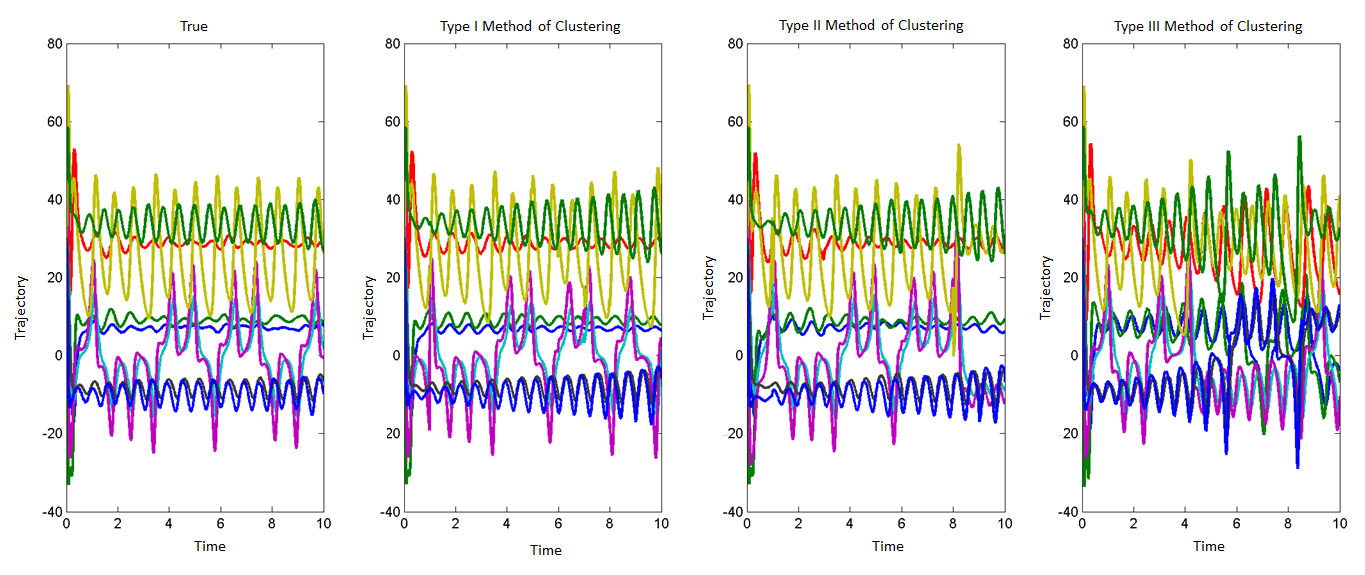
\includegraphics[scale=0.5]{figures_2/fig_comp_9dim}
}
\caption{Dimension $n= 9$, coupling strength $\epsilon= 1$}
\label{plot_9dim}
\end{figure} 


\section{Diffusively Coupled Lorenz Attractors}

The three coupled Lorenz Attractor problem in Section~\ref{three_osc} is further scaled to high dimensional systems. The equation of $N$ nonidentical and decoupled Lorenz attractors is defined by the following system of differential equation:  
\begin{equation}
\label{lorenz_coup}
\begin{array}{lc}
\dot{x}_{i} = \sigma_i (y_{i} - x_{i}) + \epsilon (x_{i+1} + x_{i-1} - 2x_{ti})  \\
\dot{y}_{i} = x_{i}(\rho_i - z_i) - y_{i} \\
\dot{z}_{i} = x_{i}y_{i} - \beta z_{i} & \hspace{5 mm}
i = 1,2,\ldots,N
\end{array} 
\end{equation} %\epsilon (x_{i+1} + x_{i-1} - 2x_{ti})

The system in Equation~\ref{lorenz_coup} is linearized and the state space is clustered following the methods described in Sections~\ref{cluster_structure} and~\ref{cluster_structure}.  Lorenz attractors exhibit chaotic properties for certain parameters. With $e = 0$, the equilibrium point for any set of parameters for an individual oscillator is $[0 \; 0 \; 0]^T$. With slight perturbation, the system repels from the equilibrium point and orients itself around two steady convection given by $\left( \pm\sqrt{\beta(\rho-1)}, \pm\sqrt{\beta(\rho-1)}, \rho-1 \right)$. To study the effectiveness of our proposed methodology, 42 test cases of the problem in Equation~\ref{lorenz_coup} are considered by taking seven values of $\epsilon = \lbrace 0.1, 1, 5, 10, 20, 50, 100 \rbrace$ and six values of $N =  \lbrace 5, 10, 25, 50, 100, 250  \rbrace $. Table~\ref{scs_weaklorenz} shows the average mean of error in propagation obtained for the three methods for some of the test cases. Lorenz system is a highly chaotic system. Hence, any slight error in wrong cluster detection can lead to an accumulation of significant error with time.

\begin{table}[H]
\caption{RMS \textit{time-averaged} mean for different test setups in Coupled Lorenz Oscillators}
\begin{center}
\resizebox{0.4\columnwidth}{!}{
\label{scs_weaklorenz}
\begin{tabular}{|c|c|c|c|c|}
\hline 
$N$ &   $\epsilon$ &   \multicolumn{3}{c|}{Type} \\ \hline
    &        &    1    &    2    &    3    \\ \hline
5    &    1    &    0.0135    &    0.0256    &    1.1243    \\ \hline
    &    20    &    0.0152    &    0.0360    &    0.3811    \\ \hline
    &    50    &    0.0175    &    0.0364    &    0.1008    \\ \hline
    &    100    &    0.0255    &    0.0386    &    0.0402    \\ \hline
10    &    0.1    &    0.0076    &    0.0093    &    3.3198    \\ \hline
    &    1    &    0.0077    &    0.0128    &    2.7919    \\ \hline
    &    5    &    0.0114    &    0.0165    &    0.8261    \\ \hline
    &    10    &    0.0106    &    0.0181    &    0.5274    \\ \hline
    &    20    &    0.0152    &    0.0188    &    0.1333    \\ \hline
25    &    0.1    &    0.0037    &    0.0043    &    1.3346    \\ \hline
    &    1    &    0.0036    &    0.0055    &    0.8408    \\ \hline
    &    5    &    0.0052    &    0.0066    &    0.1862    \\ \hline
    &    10    &    0.0051    &    0.0072    &    0.2684    \\ \hline
    &    20    &    0.0041    &    0.0074    &    0.1083    \\ \hline
    &    50    &    0.0057    &    0.0076    &    0.0234    \\ \hline
    &    100    &    0.0077    &    0.0098    &    0.0106    \\ \hline
50    &    1    &    0.0021    &    0.0028    &    0.6497    \\ \hline
    &    5    &    0.0000    &    0.0026    &    0.0033    \\ \hline
    &    10    &    0.0000    &    0.0036    &    0.0041    \\ \hline
    &    100    &    0.0039    &    0.0054    &    0.0136    \\ \hline
100    &    0.1    &    0.0009    &    0.0011    &    1.2278    \\ \hline
    &    1    &    0.0000    &    0.0009    &    0.0014    \\ \hline
    &    5    &    0.0000    &    0.0013    &    0.0017    \\ \hline
    &    10    &    0.0000    &    0.0013    &    0.0018    \\ \hline
    &    20    &    0.0019    &    0.0071    &    0.0608    \\ \hline
    &    50    &    0.0019    &    0.0058    &    0.1974    \\ \hline
\end{tabular} 
}
\end{center}
\end{table}

\section{Diffusively Coupled Van der Pol Oscillators}
The state space equations of weakly coupled Van der Pol Oscillators is given as~\cite{van1920theory}:

\begin{equation}
\label{strong_vanderpol}
\begin{array}{l}
\dot{x}_i = y_i + \epsilon (x_{i-1} - 2x_i + x_{i+1}) \\
\dot{y}_i = \mu(1-x_i^2)y_i - x_i  
\end{array}\hspace{5 mm} i = 1,2,\ldots,N
\end{equation}

The value of the $\epsilon$ is kept very low to introduce a weak coupling between the oscillators. Strong coupling induces a change in the behavior of the individual oscillator. The changing cluster structure needs to be identified with time to avoid accumulation of error. Table~\ref{strongvanderpol} shows the average mean of error in propagation obtained for the three methods for some of the test cases.

\begin{table}[H]
\caption{RMS \textit{time-averaged} mean for different test setups in Coupled Van der Pol Oscillators}
\begin{center}
\resizebox{0.4\columnwidth}{!}{
\label{strongvanderpol}
\begin{tabular}{|c|c|c|c|c|}
\hline 
$N$ &   $\epsilon$ &   \multicolumn{3}{c|}{Type} \\ \hline
    &        &    1    &    2    &    3    \\ \hline
5    &    0.1    &    0.00190    &    0.0023    &    0.00279    \\ \hline
    &    1    &    0.00339    &    0.0179    &    0.02887    \\ \hline
    &    5    &    0.00323    &    0.0075    &    0.03404    \\ \hline
10    &    0.1    &    0.00082    &    0.0012    &    0.00126    \\ \hline
    &    1    &    0.00473    &    0.0079    &    0.01142    \\ \hline
    &    5    &    0.01282    &    0.0152    &    0.02383    \\ \hline
    &    20    &    0.01937    &    0.0215    &    0.02645    \\ \hline
    &    100    &    0.02112    &    0.0228    &    0.02428    \\ \hline
25    &    0.1    &    0.00046    &    0.0006    &    0.00103    \\ \hline
    &    10    &    0.01053    &    0.0107    &    0.01106    \\ \hline
    &    20    &    0.01096    &    0.0117    &    0.01271    \\ \hline
    &    50    &    0.01131    &    0.0128    &    0.01315    \\ \hline
50    &    0.1    &    0.00028    &    0.0003    &    0.00052    \\ \hline
    &    1    &    0.00153    &    0.0032    &    0.00387    \\ \hline
    &    5    &    0.00394    &    0.0049    &    0.00492    \\ \hline
    &    10    &    0.00519    &    0.0052    &    0.00558    \\ \hline
    &    20    &    0.00539    &    0.0060    &    0.00647    \\ \hline
    &    50    &    0.00558    &    0.0068    &    0.00689    \\ \hline
100    &    1    &    0.00072    &    0.0015    &    0.00178    \\ \hline
    &    5    &    0.00187    &    0.0023    &    0.00253    \\ \hline
    &    10    &    0.00241    &    0.0026    &    0.00271    \\ \hline
    &    50    &    0.00260    &    0.0036    &    0.00383    \\ \hline
    &    100    &    0.00264    &    0.0038    &    0.00415    \\ \hline
250    &    0.1    &    0.00005    &    0.0001    &    0.00015    \\ \hline
    &    1    &    0.00001    &    0.0003    &    0.00055    \\ \hline
    &    5    &    0.00027    &    0.0007    &    0.00088    \\ \hline
    &    10    &    0.00094    &    0.0010    &    0.00106    \\ \hline
\end{tabular} 
}
\end{center}
\end{table}


\section{Diffusively Coupled Rossler Attractors}
The equation of $N$ nonidentical Rossler attractors~\cite{rossler1976equation,heagy1994synchronous} is defined by the system of following differential equation: 
\begin{equation}
\begin{array}{lc}
\dot{x}_{i} = -\omega_i y_{i} - z_{i} + \epsilon (x_{i+1} + x_{i-1} - 2x_{ti})  \\
\dot{y}_{i} = \omega_i x_{i} + a_i y_{i} \\
\dot{z}_{i} = b_i + z_{i}(x_{i} - c_i) & \hspace{5 mm}
i = 1,2,\ldots,N
\end{array}
\end{equation}
The dynamics of the $i^{th}$ oscillator follows the equation of a 3D Rossler system~\cite{rossler1976equation}. The coupling function involves the $x$ coordinates of adjacent 3 states only. For $N$ oscillators, the dimension of the problem becomes $n = 3N$. The expression for equilibrium point becomes
\begin{equation}
x_{i0} = \frac{c_i+\sqrt {{c_{{i}}}^{2}-4\,{\frac {a_{{i}}b_{{i}}}{{\omega_{{i}
}}^{2}}}}}{2} \hspace{5 mm}
y_{i0} = -\frac{\omega_i c_i+\omega_i\sqrt {{c_{{i}}}^{2}-4\,{\frac {a_{{i}}b_{{i}}}{{\omega_{{i}
}}^{2}}}}}{2a_i} \hspace{5 mm}
z_{i0} = \frac{\omega_i^2 c_i+\omega_i^2\sqrt {{c_{{i}}}^{2}-4\,{\frac {a_{{i}}b_{{i}}}{{\omega_{{i}
}}^{2}}}}}{2a_i}
\end{equation}
with $c_1 = c_2 = \ldots = c_N$ and $a_ib_i/\omega_i$ as constant for all the $N$ oscillators. Table~\ref{weakrossler} shows the mean of error in propagation obtained for the three methods for different values of $N$ and $\epsilon$. Ideally, when the state space is clustered, one may expect a cluster to contain all the $x_j,y_j$ and $z_j$ states pertaining to any $j^{th}$ oscillator, and also the number of identified clusters to be $\le N$.  In this problem too, the same test cases of seven values of $\epsilon = \lbrace 0.1, 1, 5, 10, 20, 50, 100 \rbrace$ and six values of $N =  \lbrace 5, 10, 25, 50, 100, 250  \rbrace $ have been considered.

\begin{table}[H]
\caption{RMS \textit{time-averaged} mean for different test setups in Coupled Rossler Oscillators}
\begin{center}
\resizebox{0.4\columnwidth}{!}{
\label{weakrossler}
\begin{tabular}{|c|c|c|c|c|}
\hline 
$N$ &   $\epsilon$ &   \multicolumn{3}{c|}{Type} \\ \hline
    &        &    1    &    2    &    3    \\ \hline
10    &    0.1    &    0.00498    &    0.0080    &    0.01512    \\ \hline
    &    1    &    0.00000    &    0.0251    &    0.03370    \\ \hline
    &    5    &    0.02114    &    0.0221    &    0.04808    \\ \hline
    &    10    &    0.01644    &    0.0198    &    0.05332    \\ \hline
    &    20    &    0.01395    &    0.0271    &    0.05364    \\ \hline
    &    50    &    0.00911    &    0.0457    &    0.04916    \\ \hline
    &    100    &    0.00549    &    0.0127    &    0.04623    \\ \hline
25    &    5    &    0.01070    &    0.0108    &    0.01374    \\ \hline
    &    10    &    0.00000    &    0.0101    &    0.01467    \\ \hline
    &    20    &    0.00909    &    0.0145    &    0.01629    \\ \hline
    &    50    &    0.00618    &    0.0191    &    0.03391    \\ \hline
50    &    20    &    0.00495    &    0.0068    &    0.00766    \\ \hline
    &    50    &    0.00454    &    0.0075    &    0.01513    \\ \hline
    &    100    &    0.00385    &    0.0084    &    0.00854    \\ \hline
150    &    0.1    &    0.00050    &    0.0009    &    0.00130    \\ \hline
    &    1    &    0.00163    &    0.0026    &    0.00270    \\ \hline
    &    10    &    0.00296    &    0.0031    &    0.00323    \\ \hline
    &    20    &    0.00140    &    0.0027    &    0.00318    \\ \hline
    &    50    &    0.00209    &    0.0025    &    0.00332    \\ \hline
\end{tabular} 
}
\end{center}
\end{table}

\section{1-D Shallow Water Equation}
\label{shallow_water}

\begin{figure}[H]
\centering
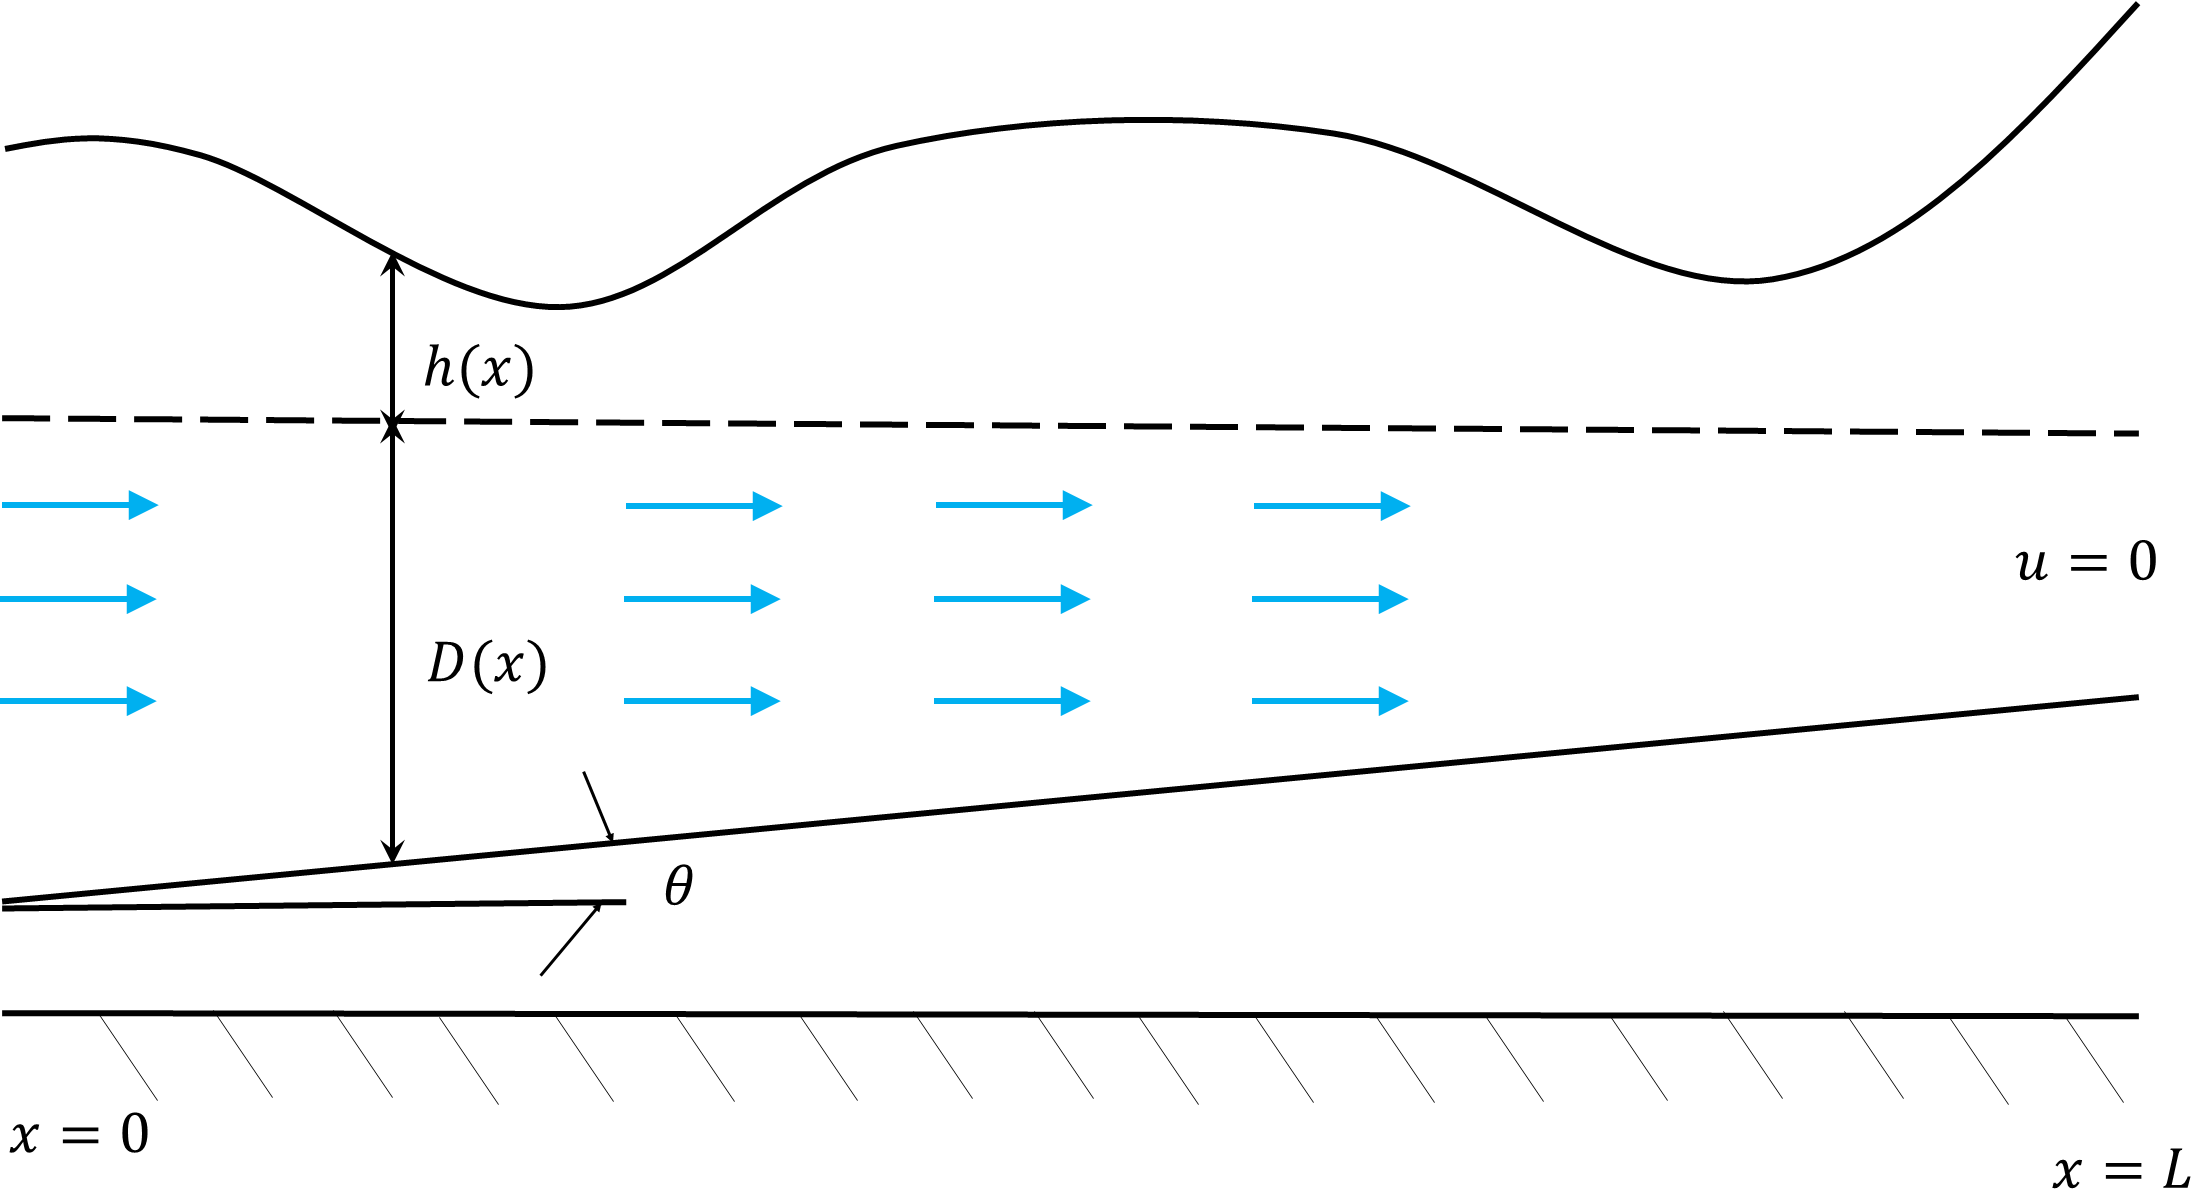
\includegraphics[scale=0.2]{figures_2/swe}
\caption{Schematic of the Tidal Water Flow}
\label{swe}
\end{figure}

The tidal water flow in a long narrow channel with varying bathymetric depth (Figure~\ref{swe}) is modeled by the Shallow Water Equations given as~\cite{verlaan1998cient}, 

\begin{equation}
\label{swe_pde}
\begin{array}{r c l}
\displaystyle \frac{\partial h}{\partial t} + D \frac{\partial u}{\partial x} + \frac{\partial D}{\partial x} u & =  & 0 \\
\displaystyle \frac{\partial u}{\partial t} + g \frac{\partial h}{\partial x} + c_f u & =  & 0 \\
h(x = 0,t) & = & h_b(t) \\
h(x ,t = 0) & = & 0 \\
u(x ,t = 0) & = & 0 \\
h(x = L ,t) & = & 0 \\
\end{array}
\end{equation}

\noindent where, $h$ denotes the water surface and $u$ is the flow velocity along the channel. The model is used to study storm surges and has been researched in details to study the effect of such surges in long narrow channels~\cite{verlaan1998cient}. The water wave is under the influence of the surge $h(0,t) = h_b(t)$. The slope is assumed as $\frac{\partial D}{\partial x} = \theta(x)$ to further simplify the system. To solve the problem, Equation~\ref{swe_pde} is discretized as per the Leendertse and Stelling scheme~\cite{verlaan1998cient,leendertse1967aspects,stelling1983construction,wesseling2009principles} as follows:

\begin{equation}
\label{swe_discrete}
\begin{array}{r c l}
\displaystyle  \frac{h_i^{k+1} - h_i^{k}}{\bigtriangleup t} + \frac{1}{2} D_i \frac{u^k_{i+\frac{1}{2}} - u^k_{i-\frac{1}{2}}}{\bigtriangleup x} + \frac{1}{2} D_i \frac{u^{k+1}_{i+\frac{1}{2}} - u^{k+1}_{i-\frac{1}{2}}}{\bigtriangleup x} +  \frac{1}{2} \theta_i \left( u^{k}_{i+\frac{1}{2}} +  u^{k+1}_{i+\frac{1}{2}} \right)  & =  & 0 \\
\displaystyle  \frac{u^{k+1}_{i+\frac{1}{2}} - u^{k}_{i+\frac{1}{2}}}{\bigtriangleup t} + \frac{1}{2} g \frac{h_{i+1}^{k} - h_i^{k}}{\bigtriangleup x}  + \frac{1}{2} g \frac{h_{i+1}^{k+1} - h_i^{k+1}}{\bigtriangleup x} + \frac{1}{2} c_f u^{k}_{i+\frac{1}{2}} + \frac{1}{2} c_f u^{k+1}_{i+\frac{1}{2}} & =  & 0 \\
h^k_0 - h_b(k \bigtriangleup t )  & =  & 0 \\
h_i^0  & =  & 0 \\
u_i^0  & =  & 0 \\
u_{N+\frac{1}{2}}^k  & =  & 0
\end{array}
\end{equation}

Equation~\ref{swe_discrete} is recast as a state space equation given by,

\begin{equation}
\label{swe_statespace}
\begin{array}{l}
\bar{D} \textbf{x}_{k+1} = \bar{A} \textbf{x}_{k} + \bar{B} \textbf{u}_k  \\
\textbf{h}_{x+1} = \bar{C} \textbf{x}_{k+1}
\end{array}
\end{equation}

where,
\begin{equation}
\label{statespace_swe}
\begin{array}{c}
\textbf{x}_k = \begin{bmatrix}
h_0^k \\ u^k_{\frac{1}{2}} \\ h_1^k \\ u^k_{1+\frac{1}{2}} \\ \vdots \\ h_N^k \\ u^k_{N+\frac{1}{2}} 
\end{bmatrix}  \hspace{5mm}
\textbf{h}_k = \begin{bmatrix}
h_0^k \\  h_1^k \\  \vdots \\ h_N^k \\ 
\end{bmatrix} \\
\bar{D} = \begin{bmatrix}
1 & 0 & 0 & 0 & 0 & \ldots & 0 \\
-\frac {g}{2\Delta x} & {\frac {1}{\Delta t}}+\frac{1}{2}\,c_{{f}} & \frac {g}{2\Delta x}  & 0 & 0 & {\ldots } & 0 \\
0 & -\frac {D_i}{2\Delta x}   & \frac {1}{\Delta t} & \frac {D_i}{2\Delta x} + \frac{1}{2}\theta_i & 0 & {\ldots } & 0 \\
\vdots & \vdots & \vdots & \vdots & \vdots & {\ldots } & \vdots \\
0 & 0 & 0 & 0 & -\frac {D_i}{2\Delta x} & \frac {1}{\Delta t} & \frac {D_i}{2\Delta x} + \frac{1}{2}\theta_i \\
0 & 0 & 0 & 0 & 0 & 0 & 1
\end{bmatrix} \\
\bar{A} = \begin{bmatrix}
0 & 0 & 0 & 0 & 0 & \ldots & 0 & 0 \\
\frac {g}{2\Delta x} & {\frac {1}{\Delta t}}-\frac{1}{2}\,c_{{f}} & -\frac {g}{2\Delta x} & 0 & 0 & {\ldots } & 0 \\
0 & \frac {D}{2\Delta x} & \frac {1}{\Delta t} & -\frac {D}{2\Delta x} - \frac{1}{2}\theta_i & 0 & {\ldots } & 0 \\
\vdots & \vdots & \vdots & \vdots & \vdots & {\ldots } & \vdots \\
0 & 0 & 0 & 0 & \frac {D}{2\Delta x} & \frac {1}{\Delta t} & -\frac {D}{2\Delta x} - \frac{1}{2}\theta_i \\
0 & 0 & 0 & 0 & 0 & 0 & 0
\end{bmatrix} \\
\bar{B} = \begin{bmatrix}
1 \\  0 \\ 0 \\ \vdots \\ 0 \\ 0
\end{bmatrix} \hspace{10mm}
\bar{C} = \begin{bmatrix}
1 & 0 & 0 & 0 & 0 & \ldots & 0  & 0 \\
0 & 0 & 1 & 0 & 0 & \ldots & 0  & 0 \\
0 & 0 & 0 & 0 & 1 & \ldots & 0  & 0 \\
\vdots & \vdots & \vdots & \vdots & \vdots & {\ldots } & \vdots & \vdots \\
0 & 0 & 0 & 0 & 0 & \ldots  & 1 & 0 \\
\end{bmatrix}
\end{array}
\end{equation}

\subsection{Results for a deterministic problem setup}
\label{deterministic}

In the deterministic test setup for Equation~\ref{swe_discrete}, the constant slope $ \theta $ in Equation~\ref{swe_statespace} is set to 0. The height of the wave at the left end is provided as an input to the equation at each time instance. The water level rises with time and the wave moves along the stretch of the channel. It then dissipates with time once the maximum height is reached. The discretized linear model in Equation~\ref{swe_statespace} is clustered by the three methods explained in Section~\ref{cluster_structure}. The adjacency matrix used in this case is $A_{sl} = \bar{D}^{-1} \bar{A}$. The parameters in Equation~\ref{swe_statespace} are assumed to be as follows:

\begin{itemize}
\item Length of the channel $L = 60$ km
\item Constant Water Depth $D = 10$ m
\item Friction constant $c_f = 0.0002$ in 1/sec
\item Total time $T = 240$ min
\end{itemize}

The discrete model in Equation~\ref{swe_discrete} is scaled using a spatial discretization of $N = 80$, with $\bigtriangleup x = L/(N+0.5)$ and a temporal discretization of $\bigtriangleup t = 300$s. Thus, the number of time steps is 80. Figure~\ref{Clustering_Types} shows the analysis of Equation~\ref{swe_statespace} using the full model and the clustered model given by the three methods of clustering. For the given test setup, Type I clustering is more effective than the other two methods of clustering. Information from one cluster is smoothly carried over to adjoining clusters via the common states. This process of information carry over is partial in Type II and absent in Type III clustering methods. 

\begin{figure}[H]
\centering
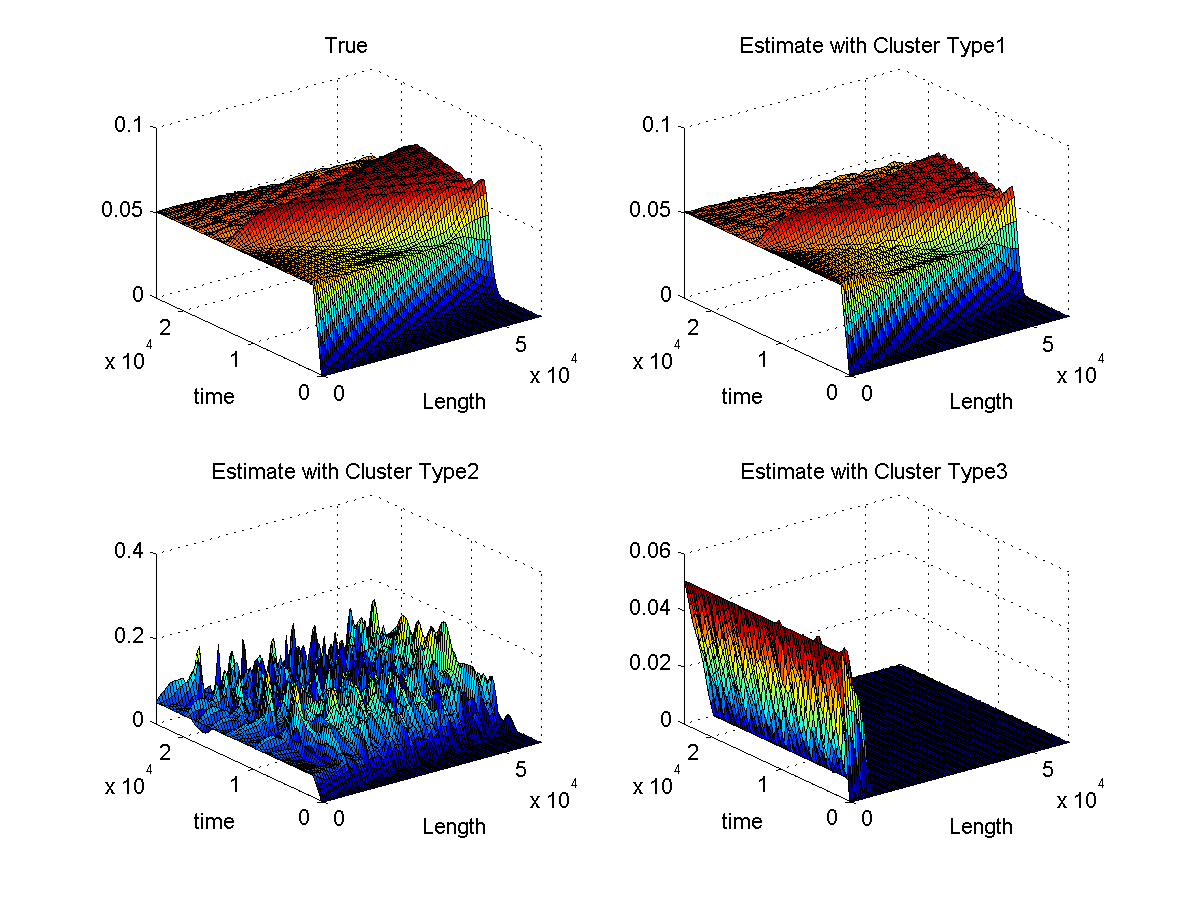
\includegraphics[scale=0.8]{figures_2/fig_comp_162_clust}
\caption{Comparison of different clustering types for a deterministic test case}
\label{Clustering_Types}
\end{figure} 

Throughout the rest of this section, Equation~\ref{swe_statespace} is solved for the same time limit of $T =  400$ mins and the length of the channel $L = 60$ km. The number of discrete spatial points $N$ has been varied from 150 to 1200, and discrete temporal points $Tstep =  T/\bigtriangleup t$ has been ranged from 60 to 1200. The stability and convergence of the discrete model are tested for the above resolutions of discretization to test the accuracy of the discrete model for solving the physical system.

\subsection{Stability Conditions}
\label{stability}
The stability conditions for a discretized model of Equation~\ref{swe_pde} is defined by the Von Neumann theory~\cite{charney1950numerical}. This condition puts a restriction on the degree of discretization for Equation~\ref{swe_discrete}. To derive the condition, following non-dimensional variables are defined:

\begin{equation}
\label{dimensionless}
\begin{array}{cccc}
\displaystyle \tilde{x} = \frac{x}{L}  & \displaystyle \tilde{t} = \frac{t}{T} & \displaystyle \tilde{h} = \frac{h}{E} & \displaystyle \tilde{u} = \frac{u}{U}
\end{array}
\end{equation} 

Thereafter, the following relations are defined:

\begin{equation}
\label{relations}
\begin{array}{cccc}
\displaystyle L^2 = DgT^2 & \displaystyle E^2 = \frac{DU^2}{g}  & \displaystyle T = \frac{\beta}{c_f} & \displaystyle \frac{TU}{E} = \alpha
\end{array}
\end{equation}

Introducing Equation~\ref{dimensionless} and~\ref{relations}, Equation~\ref{swe_pde} yields the set of following dimensionless equations:

\begin{equation}
\label{swe_dim}
\begin{array}{r c l}
\displaystyle \frac{\partial \tilde{h}}{\partial \tilde{t}} +  \frac{\partial \tilde{u}}{\partial \tilde{x}} + \theta \alpha \tilde{u} & =  & 0 \\
\displaystyle \frac{\partial \tilde{u}}{\partial \tilde{t}} +  \frac{\partial \tilde{h}}{\partial \tilde{x}} + \beta \tilde{u} & =  & 0 \\
\end{array}
\end{equation}

The solution to Equation~\ref{swe_dim} is expressed in terms of discrete Fourier modes as,

\begin{equation}
\label{fourier}
\begin{array}{l}
\tilde{h}_{i}^{k} = E^k \exp(j k_x i \bigtriangleup x) \\
\tilde{u}_{i+\frac{1}{2}}^{k} = U^k \exp(j k_x (i+\frac{1}{2}) \bigtriangleup x)
\end{array} \hspace{5mm} j^2 = -1
\end{equation}

Putting the expression for $\tilde{h}_{i}^{k}$ and $\tilde{u}_{i+1}^{k}$ into the dimensionless form of Equation~\ref{swe_discrete}, we get:

\begin{equation}
\label{fourier_mode}
\begin{array}{l}
E^{k+1} - E^{k} = -j \frac{\bigtriangleup t}{\bigtriangleup x} (U^{k} + U^{k+1}) \sin \left( \frac{k_x \bigtriangleup x}{2} \right) - \theta \alpha \frac{1}{2} \bigtriangleup t (U^{k} + U^{k+1}) \exp \left( j \frac{k_x \bigtriangleup x}{2} \right) \\
U^{k+1} - U^{k} = -j  \frac{\bigtriangleup t}{\bigtriangleup x} (E^{k} + E^{k+1}) \sin \left( \frac{k_x \bigtriangleup x}{2} \right) - \beta \frac{1}{2} \bigtriangleup t (U^{k} + U^{k+1})
\end{array}
\end{equation}

Equation~\ref{fourier_mode} is expressed in the matrix form as:

\begin{equation}
\begin{pmatrix}
E^{k+1} \\
U^{k+1}
\end{pmatrix} = 
A \begin{pmatrix}
E^{k} \\
U^{k}
\end{pmatrix}
\end{equation}

\noindent where, 
\begin{equation}
\begin{array}{l} 
A = c \resizebox{.9 \textwidth}{!}  { $ \begin{bmatrix}
-j\exp\left( j \frac{k_x \bigtriangleup x}{2} \right) \sin \left( \frac{k_x \bigtriangleup x}{2} \right) \alpha {\bigtriangleup t}^{2}\theta \bigtriangleup x
+ 2 \sin^2 \left( \frac{k_x \bigtriangleup x}{2} \right) {\bigtriangleup t}^{2} - \beta \bigtriangleup t{ \bigtriangleup x}^{2} - 2\,{ \bigtriangleup x}^{2} &  
2 \theta \alpha \bigtriangleup t \exp\left( j \frac{k_x \bigtriangleup x}{2} \right) \bigtriangleup x^2 + 4j \bigtriangleup t  \bigtriangleup x  \sin \left( \frac{k_x \bigtriangleup x}{2} \right)\\
4j \bigtriangleup t  \bigtriangleup x  \sin \left( \frac{k_x \bigtriangleup x}{2} \right) & 
-j\exp\left( j \frac{k_x \bigtriangleup x}{2} \right) \sin \left( \frac{k_x \bigtriangleup x}{2} \right) \alpha {\bigtriangleup t}^{2}\theta \bigtriangleup x  +  2 \sin^2 \left( \frac{k_x \bigtriangleup x}{2} \right) {\bigtriangleup t}^{2} + \beta \bigtriangleup t{ \bigtriangleup x}^{2} - 2\,{ \bigtriangleup x}^{2}
\end{bmatrix}$  } \\
c = \displaystyle \frac{1}{j\exp\left( j \frac{k_x \bigtriangleup x}{2} \right) \sin \left( \frac{k_x \bigtriangleup x}{2} \right) \alpha {\bigtriangleup t}^{2}\theta \bigtriangleup x
-2 \sin^2 \left( \frac{k_x \bigtriangleup x}{2} \right) {\bigtriangleup t}^{2}-\beta \bigtriangleup t{ \bigtriangleup x}^{2}-2\,{ \bigtriangleup x}^{2}
} 
\end{array} 
\end{equation}
By Von Neumann theory of stability analysis~\cite{charney1950numerical}, for a given resolution of spatio-temporal discretization or a combination of  $\bigtriangleup x$ and $\bigtriangleup t$, the system is stable if the norm of the matrix $A$ is less than 1. The discrete model in Equation~\ref{swe_discrete} has been found to be stable for all the combinations for $N$ and $\bigtriangleup t$ that have been chosen in subsection~\ref{deterministic}. 

\subsection{Convergence Analysis}

Once the discrete model is determined to be stable for a varying resolutions of discretization, the convergence analysis is performed. The discrete model is supposed to converge to the exact solution with increase in resolution. Since there is no analytic solution available, a very high resolution discretization with $N = 3200$ and $\bigtriangleup t = 15$s is chosen. The true solution for the height of the water level is given by a  $1601 \times 3201$  matrix $U_{true}$. This matrix records the height at each point along the $x$-direction for each time instance.  For a given resolution of discretization $r = (\bigtriangleup t, \bigtriangleup x)$, the same matrix $U_r$ is computed and upscaled it to the resolution of the matrix $U_{true}$ as $\hat{U}_r$. The the error rate of convergence for $r$ is calculated as,

\begin{equation}
\displaystyle \epsilon_r = \begin{Vmatrix}
\frac{U_{true} - \hat{U}_r}{U_{true}}
\end{Vmatrix}_2
\end{equation}

Figure~\ref{conv_plot} depicts the rate of convergence for different resolutions of discretization. The convergence rate decreases with increase in resolution of the discrete model.  Following the result of convergence and stability, it can be concluded that the discrete model in Equation~\ref{swe_discrete} can approximate the solution to the continuous model in Equation~\ref{swe_pde}.   

\begin{figure}[H]
\centering
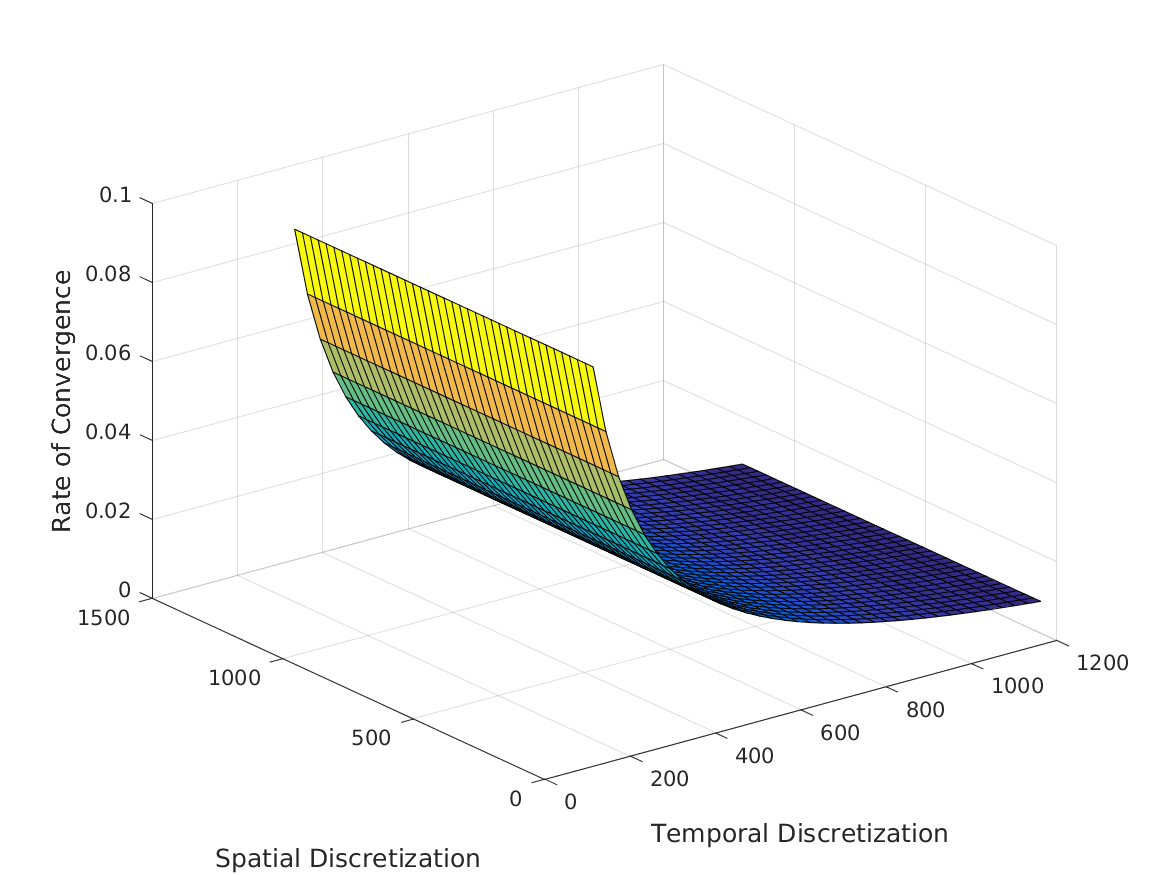
\includegraphics[width=\textwidth]{figures_2/conv_disc}
\caption{Rate of Convergence vs Discretization Resolution}
\label{conv_plot}
\end{figure}



\subsection{Cluster Length vs Resolution of Discretization}

In this section, the clusters are determined using the different methods of clustering discussed in Section~\ref{cluster_structure} for the 1-D shallow water equation~\ref{swe_discrete} to give a better physical interpretation of the state-space clusters. The state space matrix $D^{-1} A$ (Equation~\ref{statespace_swe}) is is used for clustering purpose. It is to be noted that for a given discrete point $x_k$ along the spatial domain, there are two state variables $u_i$ and $h_{i+\frac{1}{2}}$. The clustering on the $D^{-1} A$ gives us the association vectors $\textbf{z}_j$'s of the state space $\textbf{x}$ in $m$ clusters, as discussed in Section~\ref{cluster_structure}. To have a useful insight into the physical meaning of the clusters, the length of the first cluster has been chosen as the subject of interest. The length of the first cluster is given as,
\begin{equation}
\mathcal{L}_1 = \displaystyle \frac{\sum_{i=1}^{2(N+1)} \mathbb{I}_1(z_{1i}) }{2(N+1)} L \hspace{6mm} \mathbb{I}_1(z_{1i}) = \begin{cases}
1 & z_{1i} = 1 \\ 0 & \text{otherwise }
\end{cases}
\end{equation} 

The length $\mathcal{L}_1$ in kilometer represents the physical space along the channel length. Since, both $D$ and $A$ are functions of $\bigtriangleup t$ and $\bigtriangleup x$, it can be assumed that $\mathcal{L}_1$ is also a function of both $\bigtriangleup t$ and $\bigtriangleup x$.  Variation in the cluster lengths with different resolutions of discretizations is illustrated in Figures~\ref{clustlength_1} and~\ref{clustlength_2}.

\begin{figure}[H]
\centering
\begin{subfigure}[b]{0.4\textwidth}
\centering
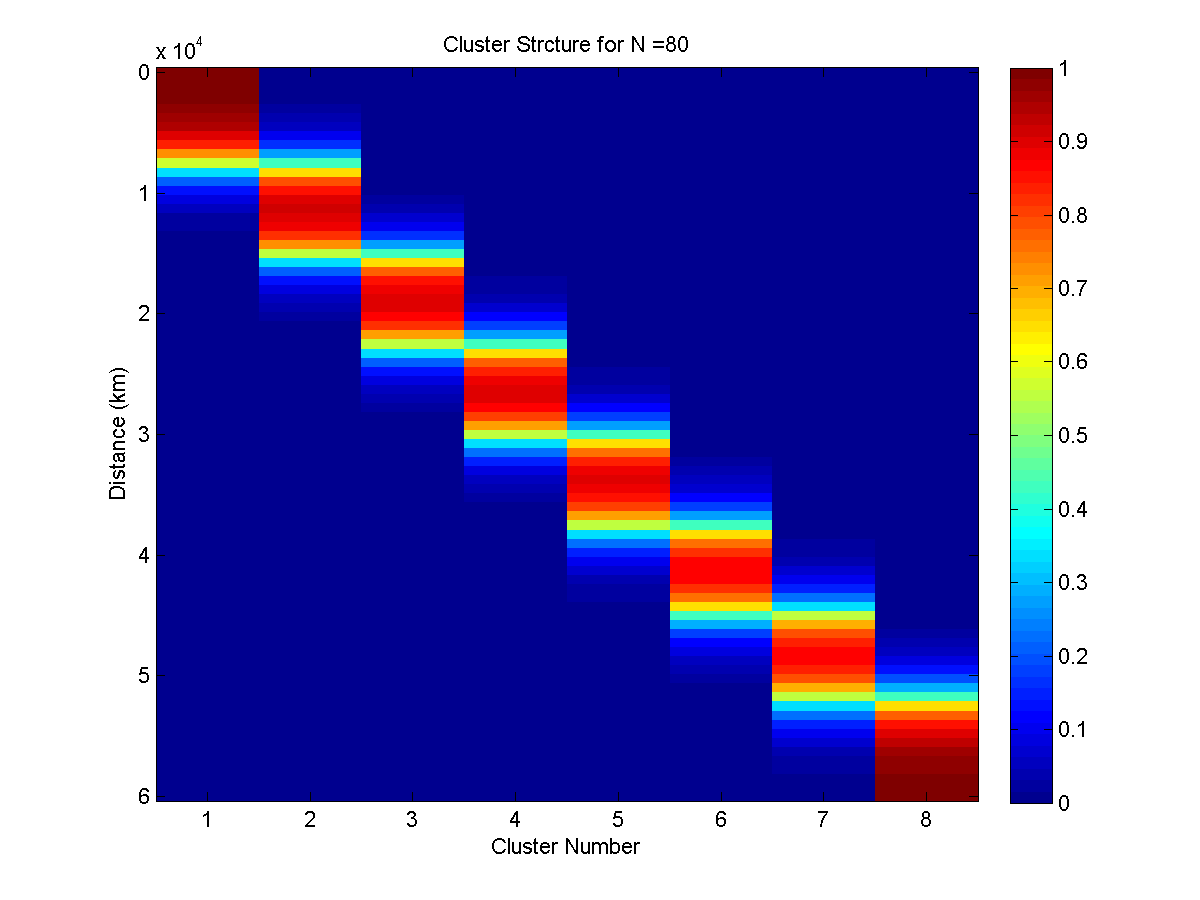
\includegraphics[width=\textwidth]{figures_2/fig_cluster_162_60_300}
\caption{Cluster Structure with N = 80}
\label{clust_N_80}
\end{subfigure}
\begin{subfigure}[b]{0.4\textwidth}
\centering
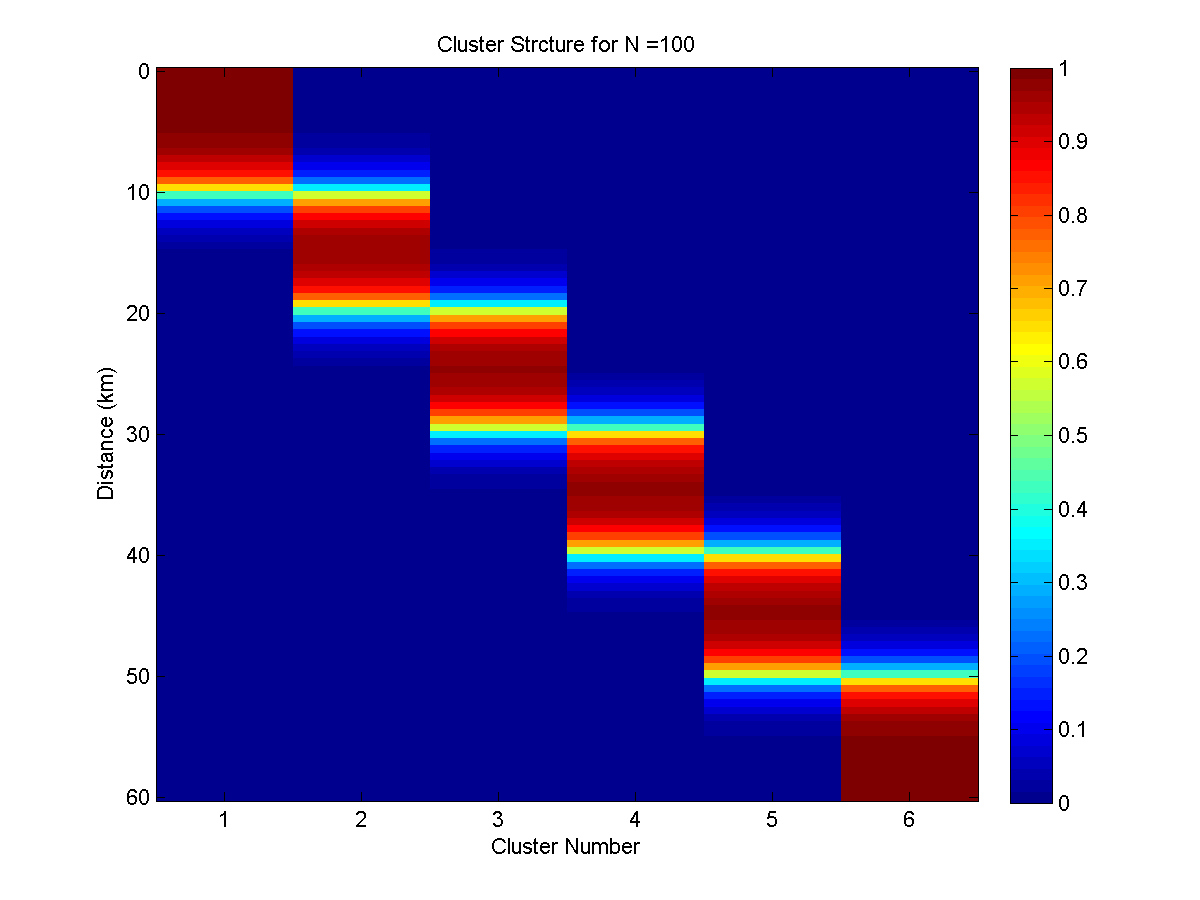
\includegraphics[width=\textwidth]{figures_2/fig_cluster_202_60_300}
\caption{Cluster Structure with N = 100}
\label{clust_N_100}
\end{subfigure}  \\
\begin{subfigure}[b]{0.4\textwidth}
\centering
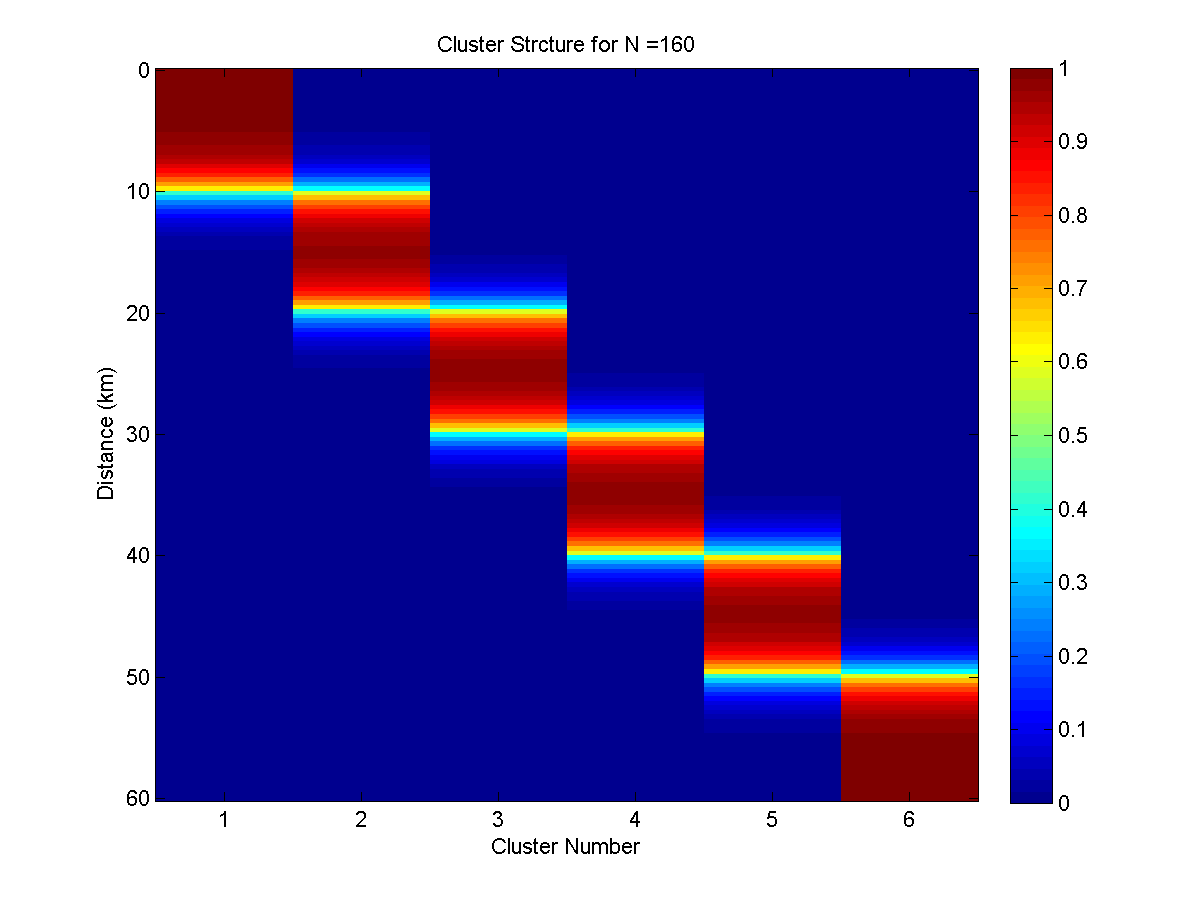
\includegraphics[width=\textwidth]{figures_2/fig_cluster_322_60_300}
\caption{Cluster Structure with N = 160}
\label{clust_N_160}
\end{subfigure}   
\begin{subfigure}[b]{0.4\textwidth}
\centering
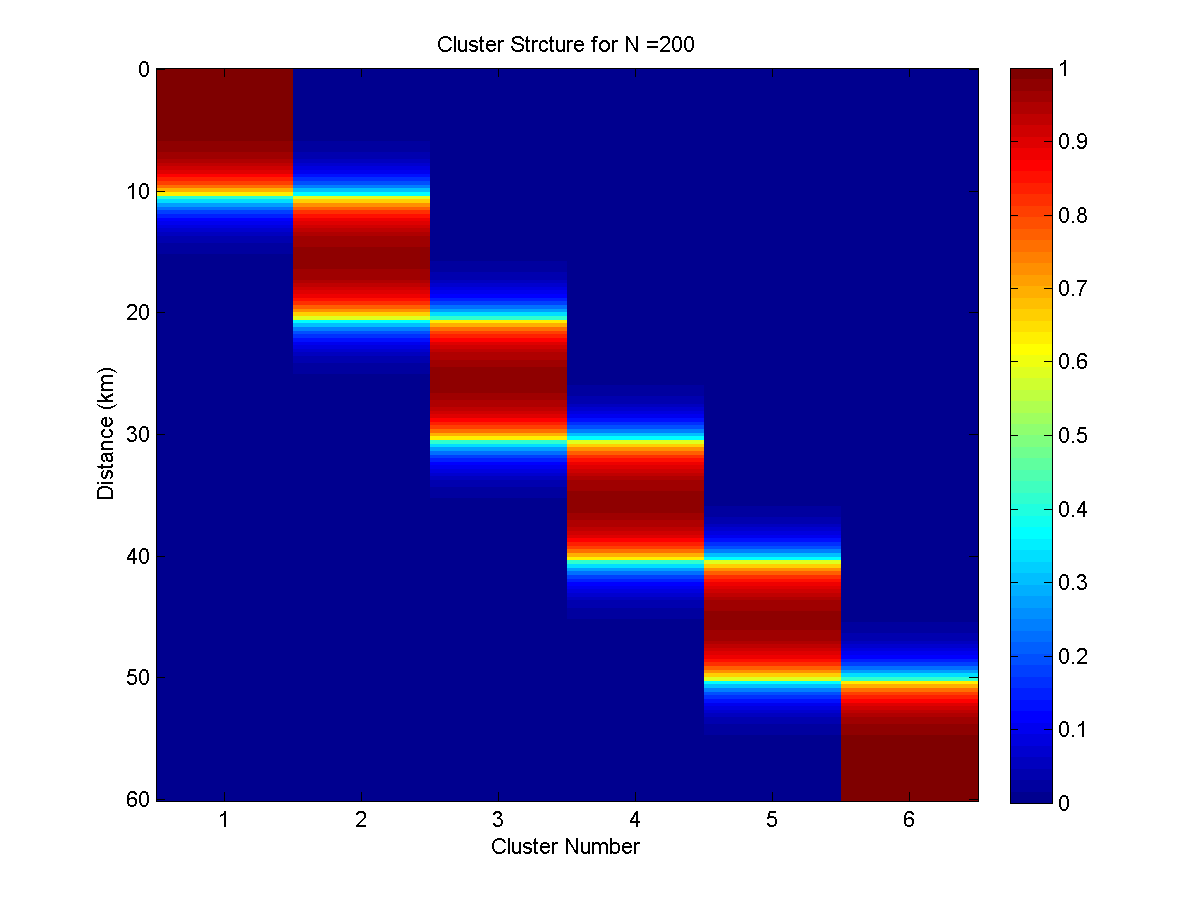
\includegraphics[width=\textwidth]{figures_2/fig_cluster_402_60_300}
\caption{Cluster Structure with N = 200}
\label{clust_N_200}
\end{subfigure}
\caption{Variation of Cluster length with varying spatial discretization and constant temporal discretization of $\bigtriangleup t = 300$s}
\label{clustlength_1}
\end{figure}

Figure~\ref{clustlength_1} shows the variation of the cluster length by varying $N = 80$ to $200$ for a constant $\bigtriangleup = 300$ s. The plots show that the cluster length is almost constant for a given $\bigtriangleup t$ and is unaffected by the change in $N$. The cluster lengths represent the physical space in which the waves can travel for a given time independent of another cluster.  This length is bound to change with an increase in $\bigtriangleup t$ or decrease in  $Tstep$.  

\begin{figure}[H]
\centering
\begin{subfigure}[b]{0.4\textwidth}
\centering
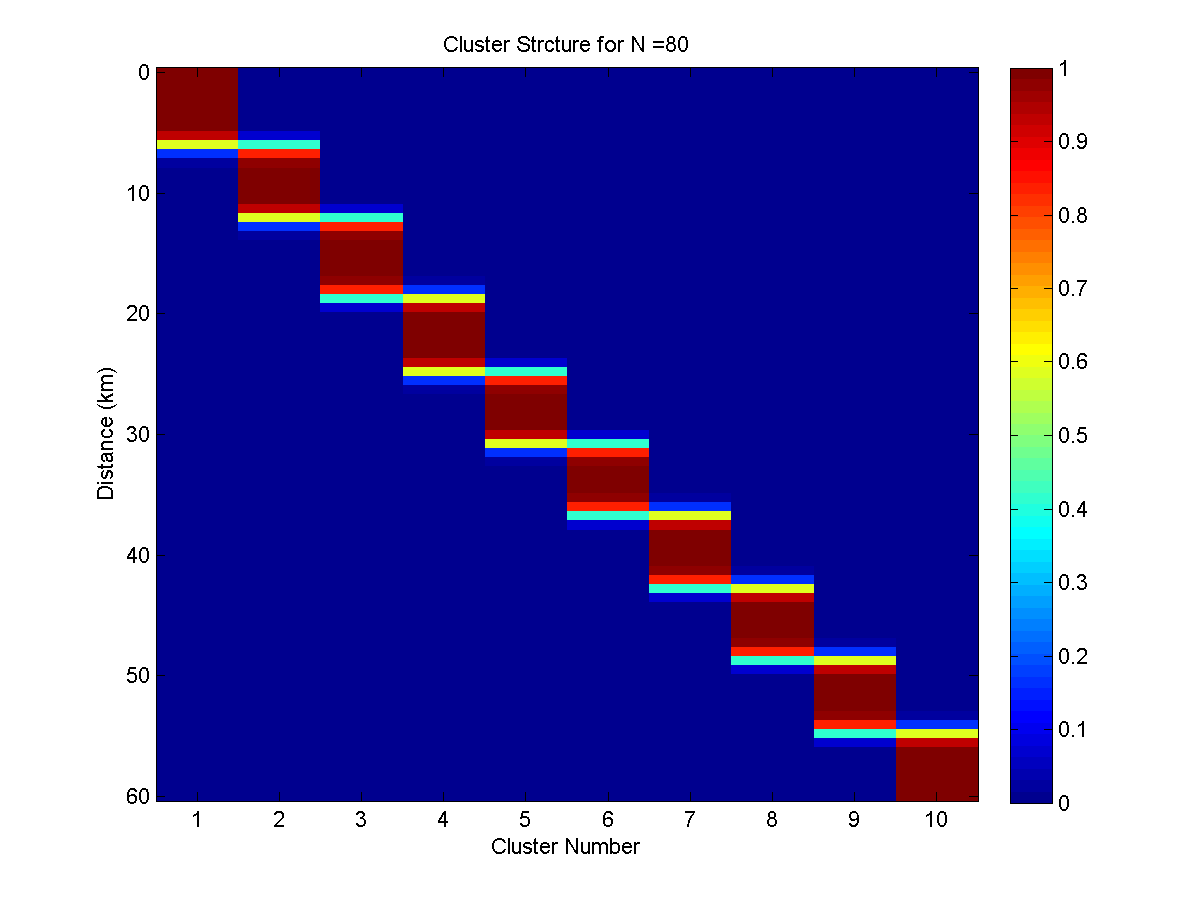
\includegraphics[width=\textwidth]{figures_2/fig_cluster_162_60_75}
\caption{Cluster Structure with $dt = 75$}
\label{clust_dt_75}
\end{subfigure}
\begin{subfigure}[b]{0.4\textwidth}
\centering
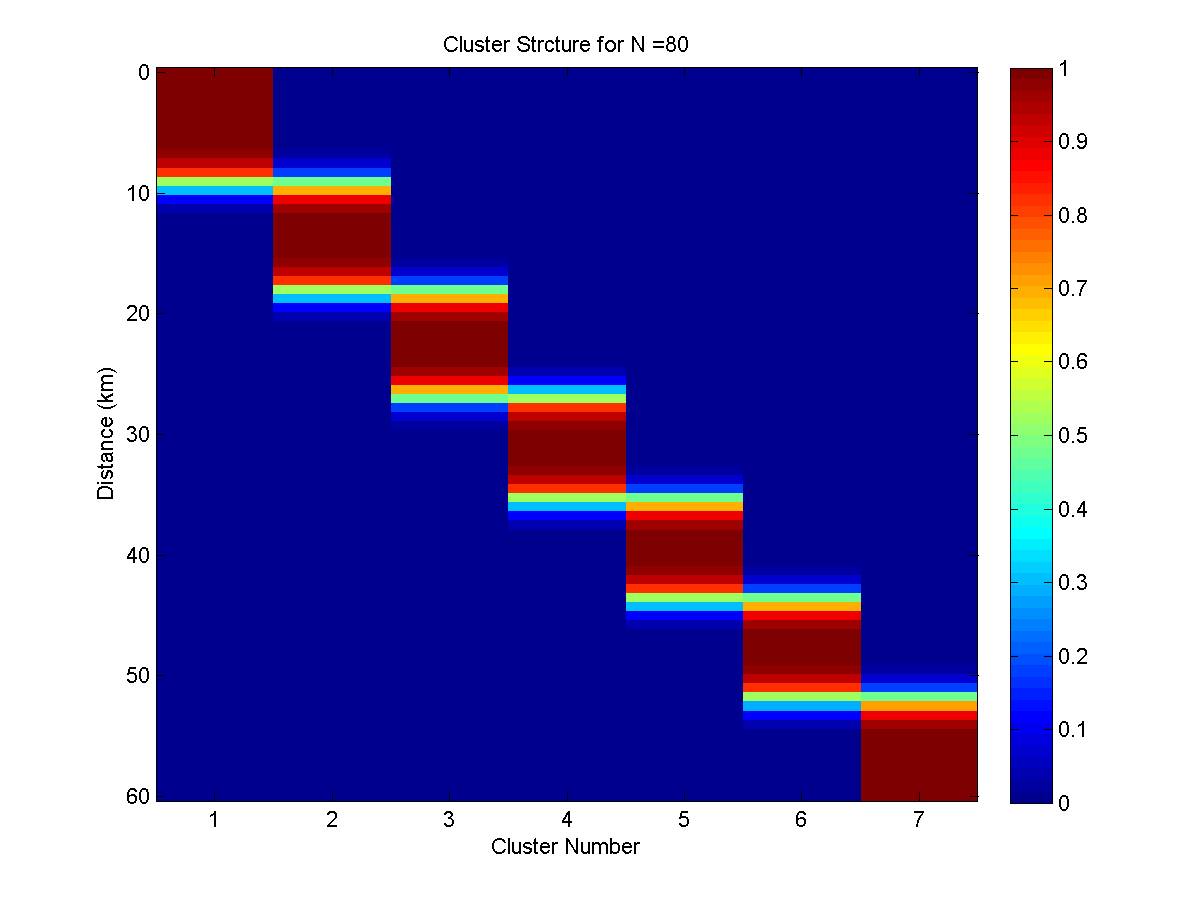
\includegraphics[width=\textwidth]{figures_2/fig_cluster_162_60_150}
\caption{Cluster Structure with $dt = 150$}
\label{clust_dt_150}
\end{subfigure}  \\
\begin{subfigure}[b]{0.4\textwidth}
\centering
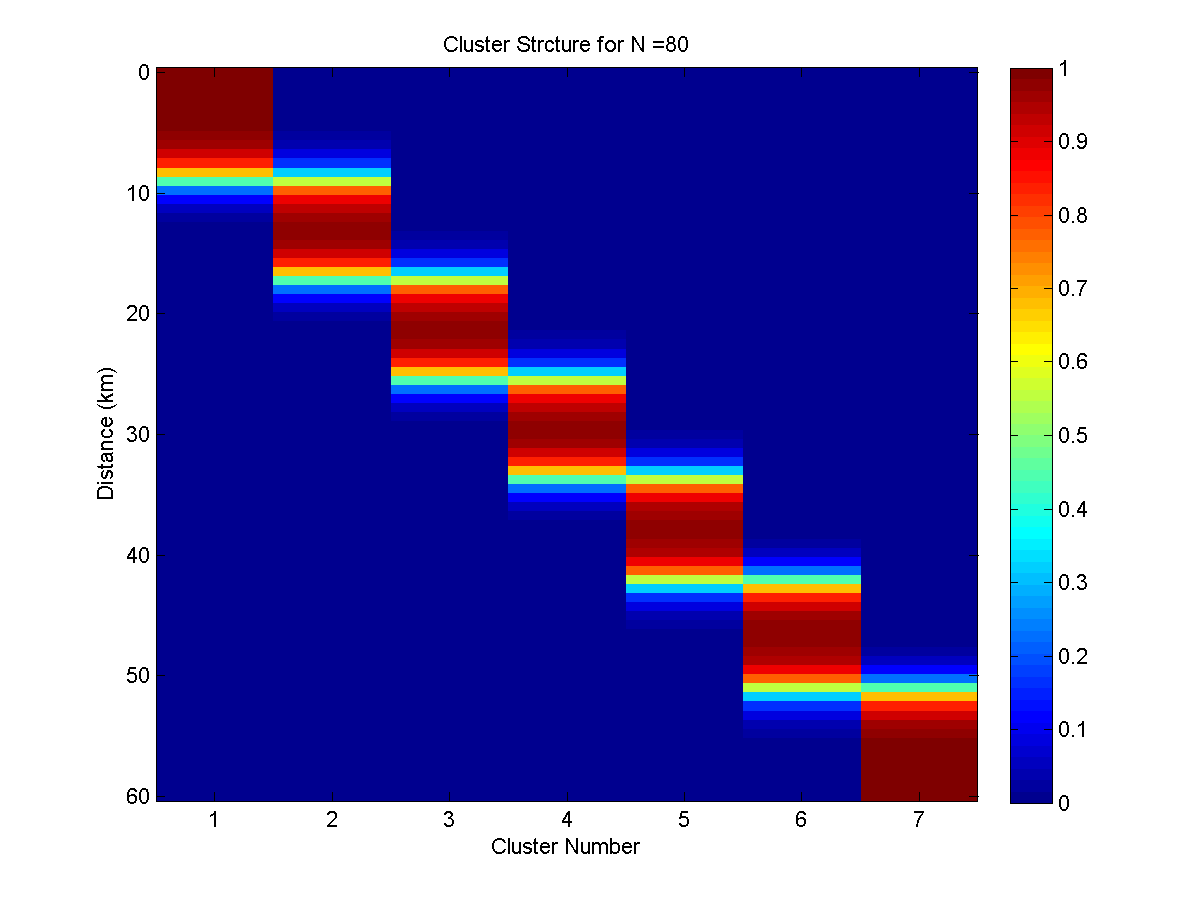
\includegraphics[width=\textwidth]{figures_2/fig_cluster_162_60_225}
\caption{Cluster Structure with $dt = 225$}
\label{clust_dt_225}
\end{subfigure}   
\begin{subfigure}[b]{0.4\textwidth}
\centering
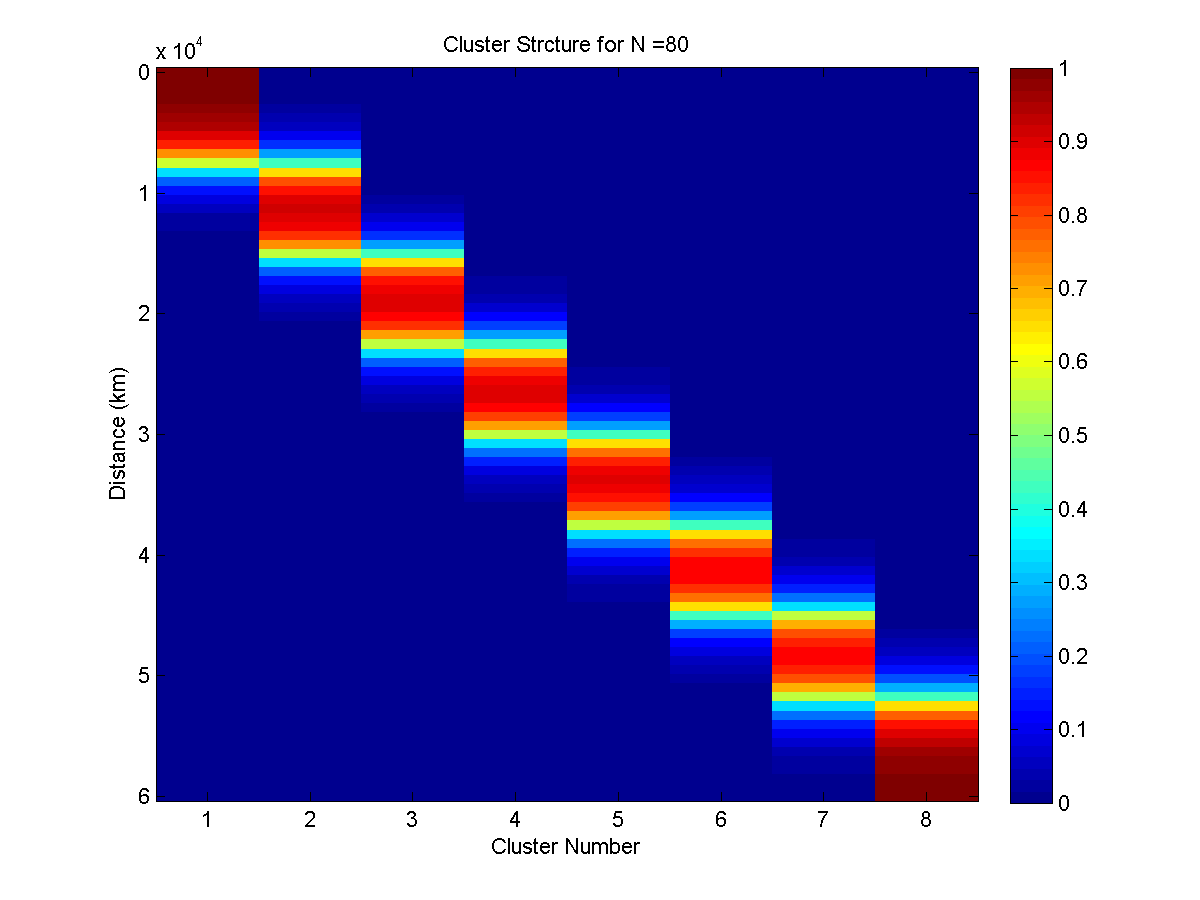
\includegraphics[width=\textwidth]{figures_2/fig_cluster_162_60_300}
\caption{Cluster Structure with $dt = 300$}
\label{clust_dt_300}
\end{subfigure}
\caption{Variation of Cluster length with constant spatial discretization $N = 80$ and varying temporal discretization}
\label{clustlength_2}
\end{figure}

Figure~\ref{clustlength_2} shows a very small variation in the values of $\mathcal{L}_1$ by varying $\bigtriangleup =  75$ to $300$s  for a constant $N = 80$. The plots show that the cluster length varies with different values of $\bigtriangleup t$. Detailed variation of the length $\mathcal{L}_1$ with change in $r$ is shown in Figure~\ref{clustlength_plot}. This analysis provides an insight into the physical meaning of the clusters. The clusters correspond to the decomposed domain that can be analyzed in parallel. The variation of the cluster lengths is consistent with the actual physical system. The subsequent UQ is carried out on the clustered model of Equation~\ref{swe_statespace} than the whole system. 

\begin{figure}[H]
\centering
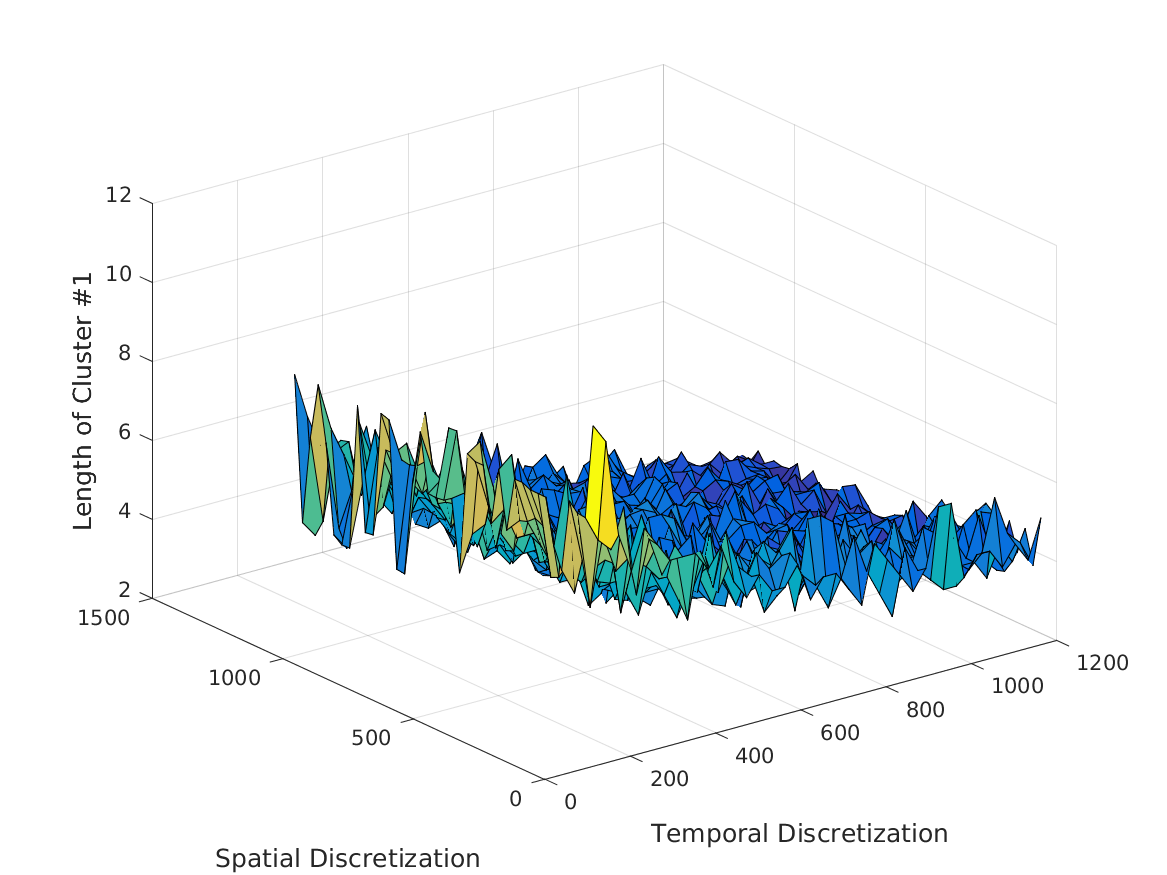
\includegraphics[width=\textwidth]{figures_2/clust_length}
\caption{Cluster Length vs Discretization Resolution}
\label{clustlength_plot}
\end{figure}


\subsection{Uncertainties associated with the model}

The bathymetric height of the system is assumed to be random for uncertainty analysis. The height and subsequently the water depth $D(x)$ is assumed to be a Gaussian random field in 1-D. The mean of $D(x)$ is assumed to have a bimodal profile shown in Figure~\ref{bathymetry} and the covariance function is assumed to be given as:

\begin{equation}
\textbf{C}(x,y) = \exp \left(-\frac{|x-y|}{a} \right)
\end{equation}

\begin{figure}[H]
\centering
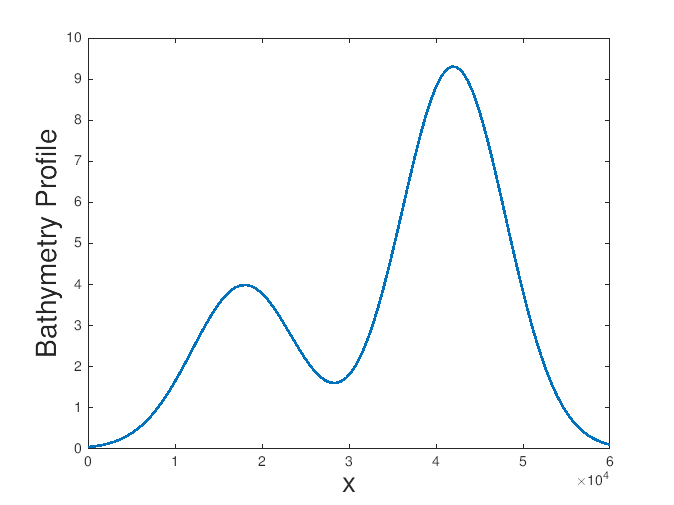
\includegraphics[scale=0.6]{figures_2/bathymetry}
\caption{Mean of the Bathymetric profile}
\label{bathymetry}
\end{figure}

$D(x)$ admits a spectral decomposition by the Karhunen-Loeve (KL) expansion as~\cite{ghanem2003stochastic}:

\begin{equation}
\label{kl_exp}
D(x)  = \mu(x) + \sum_{i=1}^\infty \sqrt{\lambda_i}\psi_i(x)D_i(x)
\end{equation}

\noindent where, $Y \sim \mathcal{N}(0,1)$ are i.i.d Gaussian random variables and $\lambda_i, \psi(x)$ are the solution to the eigenvalue problem:

\begin{equation}
\int_0^L \textbf{C}(x_1,x_2) \psi_i(x_2) dx_2 = \lambda_i \psi_i(x_1)
\end{equation}

The expansion of Equation~\ref{kl_exp} is truncated according to the decay of the eigenvalues $\lbrace \lambda_i \rbrace$s. The random field $D(x)$ is expressed in terms of the first $M$ eigenvalues as:

\begin{equation}
D(x)  = \mu(x) + \sum_{i=1}^M \sqrt{\lambda_i}\psi_i(x)D_i(x)
\end{equation} 

The eigenvalue trend for $a = 0.1L$ is depicted in Figure~\ref{eigenvalue}. This trend helps in truncating the expression of KL expansion. From the figure, $M$ can be approximated as 12. 


\begin{figure}[H]
\centering
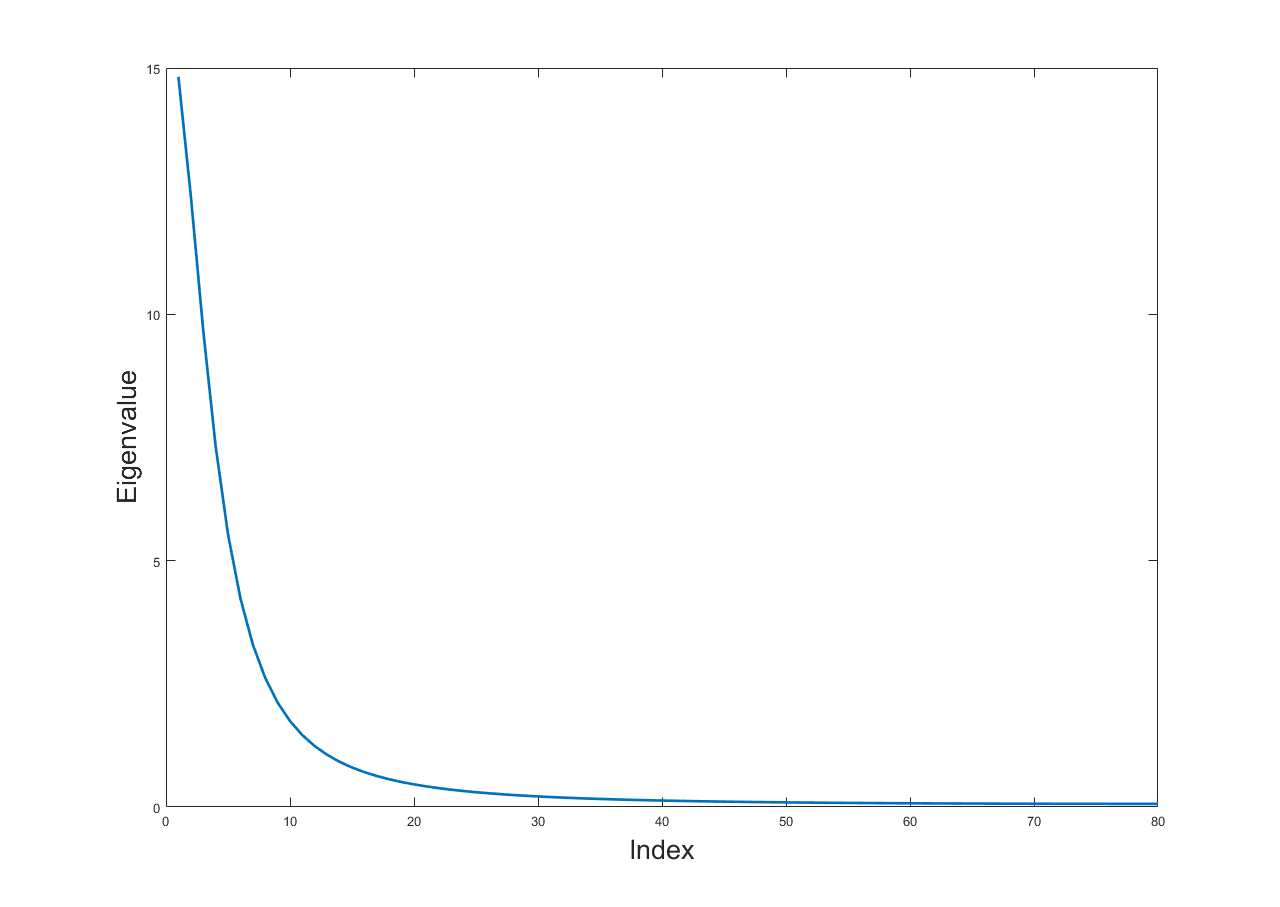
\includegraphics[scale=0.4]{figures_2/eigenvalue}
\caption{Trend of Eigenvalue for exponential covariance function with $a = 0.1L$}
\label{eigenvalue}
\end{figure}


Measurements for $\textbf{h}_{k}$ are generated using the deterministic model explained in the Section~\ref{deterministic}.  The following section details the method of clustering and UQ applied to estimate the uncertainties in the state $\textbf{h}_{k}$ and $\textbf{u}_k$.

\subsection{Clustering and Uncertainty Quantification}
 
 The state space of the model includes the discretized height of the water level $\textbf{h}_{k}$ and the velocity $\textbf{u}_k$.  The uncertainty in $\textbf{h}_k$ and $\textbf{u}_k$  is attributed to $D(x)$ and the initial state uncertainty. To cluster the state space, the statistically linearized matrix is obtained from the state-space Equation~\ref{swe_statespace}, as follows:
 
 \begin{equation}
 A_{sl}  = \int_0^L \bar{D}^{-1} (D(x)) \bar{A} (D(x)) dP_{D(x)}
\end{equation}  

For simplicity, the linearized matrix is assumed as $A_{sl} = \bar{D}^{-1} \left(E \left[ D(x) \right]\right) \bar{A} \left(E \left[ D(x) \right]\right) $. For $N=80$ and $\bigtriangleup t = 300$s, the cluster structure of $A_{sl}$ is shown in Figure~\ref{cluster_samp}. The clustering output results in five almost equal sized clusters. The clustering decomposes the 1-D domain into five overlapping domains $D_j, j=1,2,\ldots,5$. Hence, the bathymetric profile is also decomposed into five random fields. 

\begin{figure}[H]
\centering
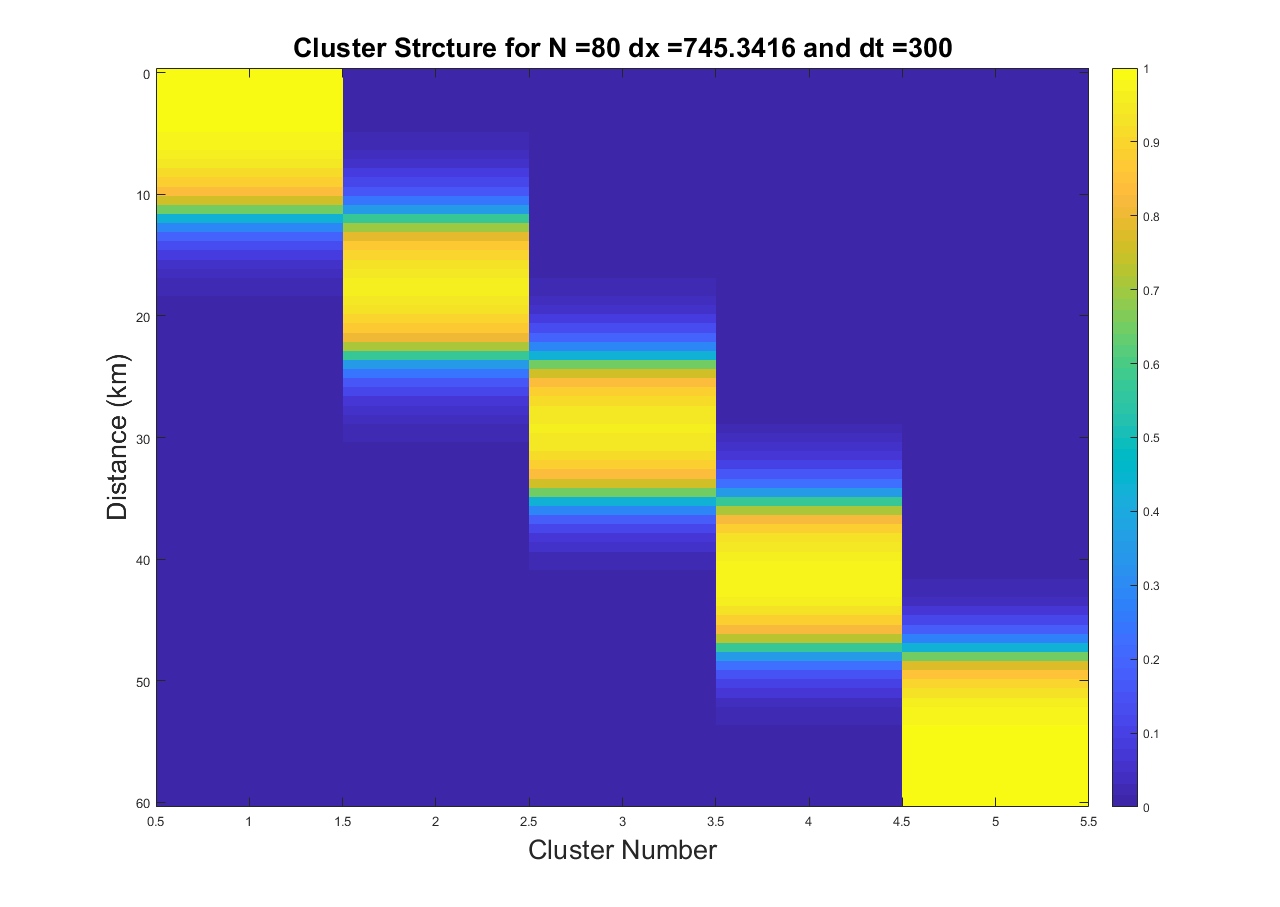
\includegraphics[scale=0.4]{figures_2/samp}
\caption{Cluster Structure for Shallow Water Model for uncertain bathymetry}
\label{cluster_samp}
\end{figure}

The effect of clustering the state space is reflected in the eigenvalue plot of the clustered random field. Figure~\ref{eigenvalue_cluster} shows the eigenvalue plot for the bathymatry random field clustered into five overlapping fields. It is observed that each cluster requires less number of eigenvalue for the truncated expansion for the random field. For each cluster $j$, the bathymetry for the domain $D_j$ can be expressed as:

\begin{equation}
D_j(x) = f(x) + \sum_{i=1}^{M_j } \sqrt{\lambda_i}\psi_i(x)D_i(x) \hspace{5 mm} x \in D_j
\end{equation}

The value of $M_j$ is approximately 4 for each cluster. This clustering reduces the total number of samples required for the random field generated by any standard quadrature method that is used to estimate high order moments. The state variables corresponding to the water level $\textbf{h}_{k}$ and the velocity $\textbf{u}_k$ are also clustered. The number of states in each cluster can be estimated from Figure~\ref{cluster_samp}.   

\begin{figure}[H]
\centering
\begin{subfigure}[b]{0.4\textwidth}
\centering
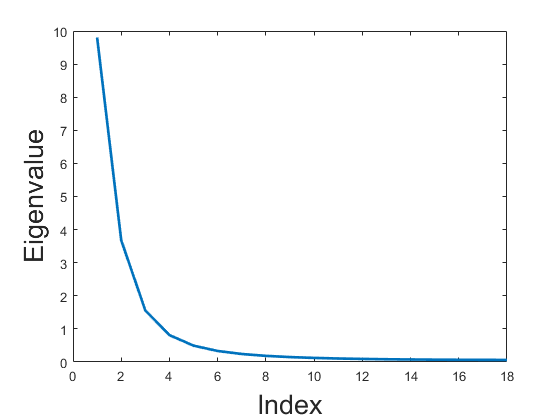
\includegraphics[width=\textwidth]{figures_2/eig1}
\caption{Cluster I}
\end{subfigure}
\begin{subfigure}[b]{0.4\textwidth}
\centering
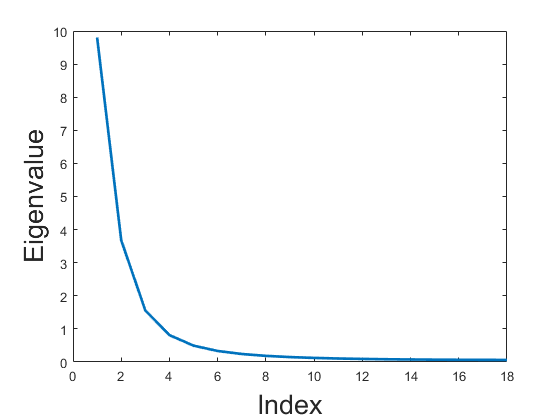
\includegraphics[width=\textwidth]{figures_2/eig2}
\caption{Cluster II}
\end{subfigure}  \\
\begin{subfigure}[b]{0.4\textwidth}
\centering
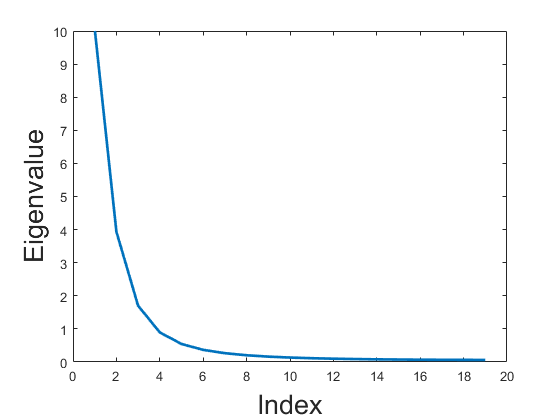
\includegraphics[width=\textwidth]{figures_2/eig3}
\caption{Cluster III}
\end{subfigure}   
\begin{subfigure}[b]{0.4\textwidth}
\centering
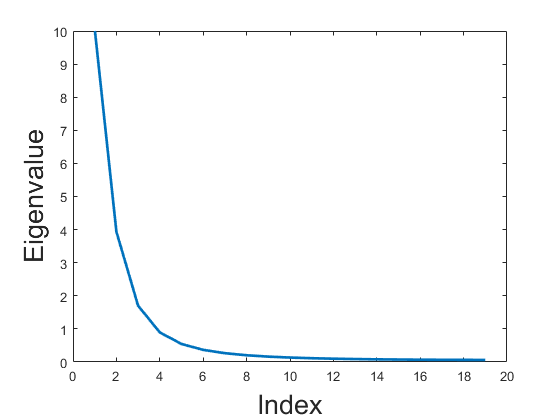
\includegraphics[width=\textwidth]{figures_2/eig4}
\caption{Cluster IV}
\end{subfigure}   \\
\begin{subfigure}[b]{0.4\textwidth}
\centering
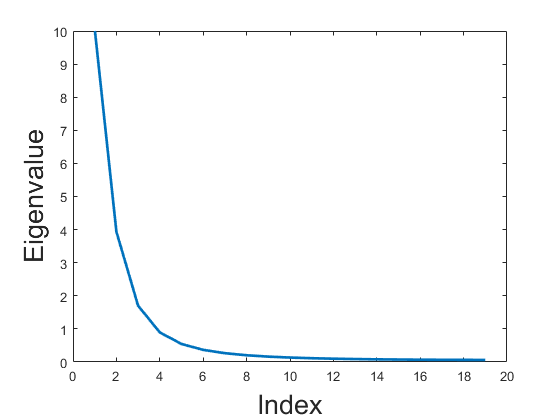
\includegraphics[width=\textwidth]{figures_2/eig5}
\caption{Cluster V}
\end{subfigure}   
\caption{Eigenvalue plot for the bathymetry random field clustered into 5 overlapping fields}
\label{eigenvalue_cluster}
\end{figure}


Corresponding filtering problem is solved as described in the Section~\ref{ukf_clust}. The effect of filtering is displayed by plotting the observed and estimated height with the $\pm 3\sigma$ limit. Figure~\ref{filterplot} shows the results of filtering out of noise with the availability of measurement. The Type I method of clustering outperforms the other two methods. While Type II and III are efficient in estimating the state, the accuracy in covariance estimation is relatively weak. 

\begin{figure}[H]
\centering
\begin{subfigure}[b]{0.3\textwidth}
\centering
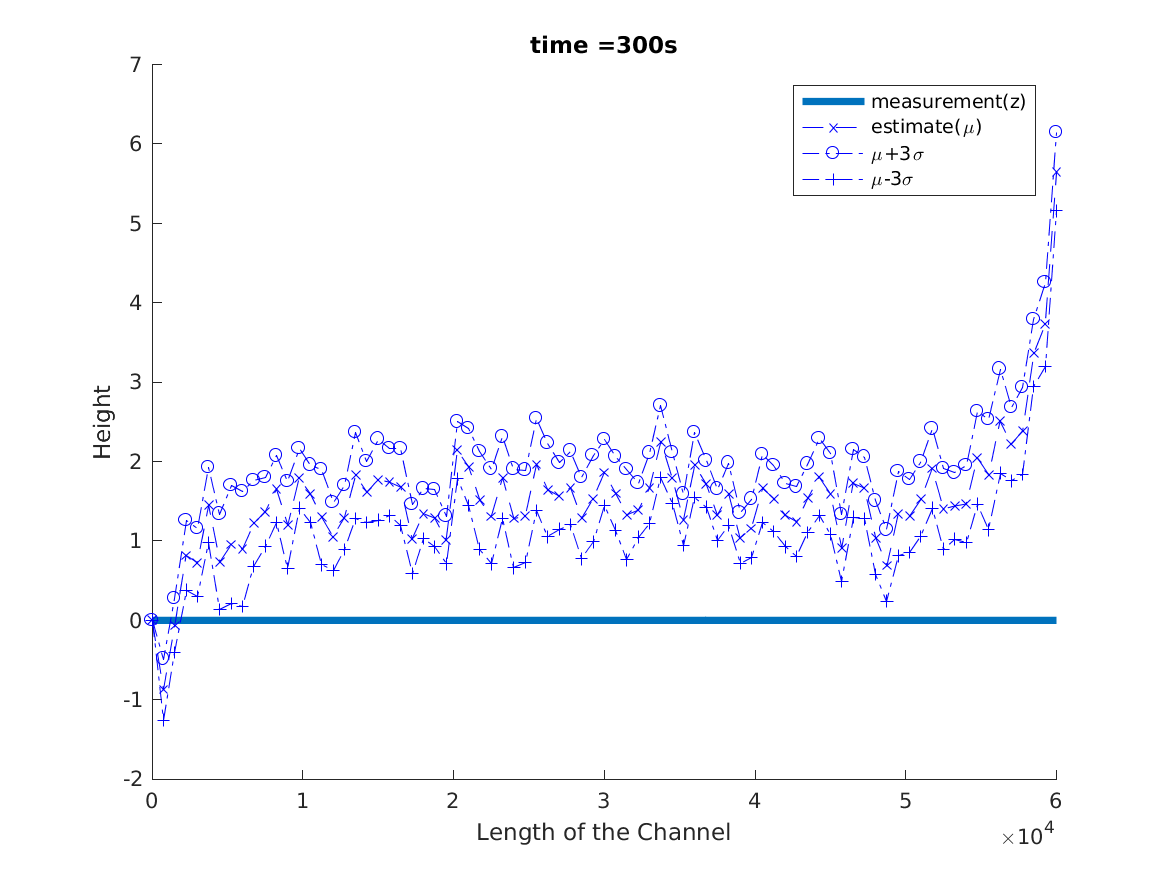
\includegraphics[width=\textwidth]{figures_2/fig11}
\caption{Cluster Technique I}
\end{subfigure}
\begin{subfigure}[b]{0.3\textwidth}
\centering
\includegraphics[width=\textwidth]{figures_2/fig21}
\caption{Cluster Technique II}
\end{subfigure} 
\begin{subfigure}[b]{0.3\textwidth}
\centering
\includegraphics[width=\textwidth]{figures_2/fig31}
\caption{Cluster Technique III}
\end{subfigure}   \\
\begin{subfigure}[b]{0.3\textwidth}
\centering
\includegraphics[width=\textwidth]{figures_2/fig131}
\caption{Cluster Technique I}
\end{subfigure}   
\begin{subfigure}[b]{0.3\textwidth}
\centering
\includegraphics[width=\textwidth]{figures_2/fig231}
\caption{Cluster Technique II}
\end{subfigure}   
\begin{subfigure}[b]{0.3\textwidth}
\centering
\includegraphics[width=\textwidth]{figures_2/fig331}
\caption{Cluster Technique III}
\end{subfigure} \\
\begin{subfigure}[b]{0.3\textwidth}
\centering
\includegraphics[width=\textwidth]{figures_2/fig171}
\caption{Cluster Technique I}
\end{subfigure}   
\begin{subfigure}[b]{0.3\textwidth}
\centering
\includegraphics[width=\textwidth]{figures_2/fig271}
\caption{Cluster Technique II}
\end{subfigure}   
\begin{subfigure}[b]{0.3\textwidth}
\centering
\includegraphics[width=\textwidth]{figures_2/fig371}
\caption{Cluster Technique III}
\end{subfigure}
\caption{Results of the filtering problem. The noise is filtered out with availability of measurement}
\label{filterplot}
\end{figure} 

\section{Summary}

This chapter formulates three different type of clustering methods to identify Strongly Coupled Subsystems (SCSs) in a high-dimensional uncertain dynamical systems. Two new methods of clustering the state-space are developed based on overlapping community detection algorithms. The third method uses the overlapping information and maps to a non-overlapping sets of community based on maximum participation of a state in a cluster. The decomposition of state-space based on outlined clustering methods facilitates effective UQ of a high-dimensional  system with fewer sample points with the help of any standard UQ method. 
The Type I method of linearization and clustering shows to be very effective in identifying the common states. The propagation method gives relatively lower error when compared with the two other methods. Type III clustering method gives us the highest error. The error for Type II is in between Type I and Type III. The error difference is more significant for the shallow water equation example.  The SWE model is carefully chosen for analysis in which the input at one end is propagated throughout the model. Hence, a proper communication between the clusters is essential to have the continuous flow of information in between two neighboring clusters over time. This communication is established very well by Type I method and not so well by Type II and III. 

%\textit{How to decide on the clustering method?}

The decision to choose a clustering method should be taken based on the problem and physical properties of the system. From the results, it is evident that the choice of clustering method does not create a significant difference on the results of the oscillator problems. The decision of selecting a clustering method is taken based on the balance between error estimate and the computation time required. It is evident that Type I method will need much more time since during the UQ all the states in the cluster are propagated. In Type I method the propagation equation in the cluster involves a higher number of state variables than the other methods. Type II method has the same number of cluster length as Type III, with the additional common states taken as input variables. Thus, Type II provides an accuracy close to Type I, while the time required during the UQ phase is much less. Also, Type II adjusts its cluster structure with varying coupling strengths for scalable problems. As pointed out earlier, Type II method shows similar cluster structure and hence accuracy as Type I method for high values of coupling strength $\epsilon$. Type III requires the least computation time but is also the least accurate. It has been shown in our earlier work, that for weak coupling Type III provides considerable accuracy. 


\chapter{Identifying Weakly Connected Subsystems in Building Energy Model (BEM) for Effective Load Estimation}
\label{chap:building}

\section{Introduction}
In 2016, the building sector used approximately 40\% of the energy produced in the United States~\citep{useia2017}, and in 2009, buildings contributed 2,184.6 million metric tons of carbon dioxide equivalent of greenhouse gases due to emissions~\citep{useia2009}.  As a result, governments and municipalities have committed to reducing the energy consumption of buildings.  New York State, for example, enacted Executive Order 88, which requires government buildings to reduce energy consumption by 20\% \citep{statedirect}, and the Public Service Commission in New York has established a public fund to target energy efficiency measures~\citep{nyspublic}. 

It is necessary to estimate the expected energy usage of a building to determine how to reduce energy usage. The expected energy usage of a building can be faithfully simulated using a Building Energy Model (BEM). Currently, there are several popular options for software to estimate the dynamic energy use, such as EnergyPlus, eQUEST, TRACE 700, and Carrier HAP~\citep{Eplus,hirsch2006equest, trace, HAP}, each of which utilizes a complex algorithm, built upon the heat-balance method, to calculate building loads. The BEMs incorporate energy load estimation due to the presence of HVAC systems, lights, and receptacle loads, and requires a substantial number of input parameters.   

Many of the numerous input parameters in a BEM are uncertain.  Some of these parameters are measured, while the owner, designer, or modeling professional must estimate others, and some are assumed by the BEM itself.  In each case, uncertainty is brought into the modeling results.  These uncertainties in the BEM can be categorized into two types: uncertainties in the measured parameters and the uncertainty in modeling~\citep{ding2015uncertainty,sun2015quantification}. To ensure that the building simulation is sufficiently accurate, and to better understand the impact of imprecisions in the input parameters and calculation methods, it is desirable to quantify uncertainty in the BEM throughout the modeling process. Uncertainty quantification (UQ) typically requires a large number of simulations to produce meaningful data, which, due to the vast number of input parameters and the dynamic nature of building simulation, is computationally expensive~\citep{rysanek2013optimum,eisenhower2012uncertainty}. We must, therefore, UQ in BEMs to a less computationally expensive model.

To enable computationally efficient UQ of BEM, following main contributions are made in this chapter:

\begin{itemize}
\item Adaptation of lumped resistor-capacitance network model to generate reduced order differential equation for BEM simulation
\item Usage of a gray-box method in conjunction with black-box Kalman filter to enable BEM parameter estimation
\item Application of WCSs identification-based UQ framework developed in Chapter~\ref{chap:wcs} to propagate the quantifiable uncertainty in the BEM.
\end{itemize}

Next, all the three main contributions are further elaborated.

The well-established technique of a lumped resistor-capacitor network is used to calculate the reduced-order zone heat balance equations. The RC method assumes that the components of the zone load can be estimated by a discrete number of resistances and capacitances, and the system is treated as equivalent to an electrical circuit~\citep{vivian2017evaluation}. In particular, the heat transfer due to the zone envelope can be reduced to a three resistance, two capacitance (3R2C) thermal network. With the RC network, one can reduce the load calculations to first-order differential equations that provide a suitable framework to carry out UQ in BEMs. 

The BEM simulation can be carried out using one of the three main models~\citep{he2016simplified,perera2014modeling}:

\begin{enumerate}
\item \textit{White box models:} In white box models detailed information about the known physical process is used to predict the future states.
\item \textit{Black-box models:} In black-box models measured data is used to estimate non-physical parameters that abstractly represent the BEM performance.
\item \textit{Gray-box models:} Gray-box models combine both the white-box and black-box methods through the use of a reduced order model with known building properties for modeling the physical process. Such models can also be easily combined with Kalman filtering to enable parameter estimation. Usage of gray-box models reduces computation time while improving the accuracy of predictions.
\end{enumerate}

Because of a large number of input parameters, despite the use of reduced order model, the resulting filtering problem is computationally expensive. The novel method of identifying Weakly Connected Subsystems (WCSs)~\citep{mukherjee2015laplacian,mukherjee2015non} is used to address this problem of performing UQ in the BEM. WCS-based UQ approach allows us to group coupled parameters to minimize the associated computation time required while continuing to propagate the quantifiable uncertainty present in the BEM. The overall approach is described in detail (later in this chapter). The optimal estimation problem to estimate parameters for UQ of BEM is the heart of this chapter.

A representative case study, a well-documented building, located in Central New York is used for modeling purposes. The created simulated model of the represented building allows us to treat many of the inputs as known parameters, with some initial uncertainty. 
%Internal loads, however, such as occupancy and receptacle loads, are difficult to assume with accuracy, as explained later in this work, so we use the measured data in an optimization routine to estimate the values.  Similarly, solar radiation is not measured in real time at the building site and can be loosely calculated based on historical solar data, but for accuracy, solar heat gain is also a good candidate for parameter estimation.
A reduced order model with a robust parameter estimation tool allows us to enable Model Predictive Control (MPC).  With MPC, the measured states of the building are used in conjunction with the predictive model.  At each sampling interval, the program performs an optimization algorithm to determine how the HVAC system should respond to the current building conditions~\citep{kelman2013analysis}.
%In this work, we investigate treating the supply air temperatures delivered by the HVAC system as unknown, and use the optimal estimation method to determine the required fan-coil output temperatures.

\section{Related Works}
\label{literature}
\subsection{Lumped capacitance RC network }
The lumped capacitance RC network reduced-order model method has been reliably used in a diverse assortment of research work to estimate the heat transfer due to the building envelope ~\citep{ramallo2013lumped,vsiroky2011experimental,li2017development}.  Further precision has been incorporated into the RC network by using dynamically estimated capacitances ~\citep{jara2016new} and second-order thermal network models ~\citep{underwood2014improved}.  The physics-based Three resistor-Two Capacitance (3R2C) model has been shown to be sufficiently accurate for approximating building models ~\citep{kircher2015lumped} based on parameters with physical meaning. In the outlined work, 3R2C models are used for modeling purpose.

Expanding the scope of the RC method, the lumped capacitance method has been used to estimate other factors affecting the thermal zone heating and cooling requirements.  The thermal mass of the zone, in particular, can be modeled with an RC network ~\citep{perera2014modeling,wang2006parameter}.  When these values are significant, long-wave radiation ~\citep{he2016simplified} and convective heat between zones ~\citep{goyal2011identification} can be modeled as black-box data-driven estimations.  Internal loads, especially, have been estimated using a filtering method in conjunction with the RC method for the surfaces ~\citep{o2010model}.

The existing literature related to the RC method are inadequate for modeling large-scale problems due to high computational cost. This computational cost is exacerbated due to increase in the number of inputs. Thus, a key contribution is in the development of a computational method to expedite the UQ using the idea of \textit{divide and conquer}.  


\subsection{Uncertainty Quantification in BEMs}

Uncertainty Quantification (UQ) is becoming more prevalent in the BEM domain, as building simulation software and methods continue to evolve~\citep{woloszyn2017treating}. Research in the field of UQ in BEM is growing at a fast pace. As explained earlier, uncertainty in a BEM can arise due to the modeling process or uncertainty in the parameters. All BEMs necessarily make assumptions to simplify the modeled building. Simplifying the assumptions in the building energy simulation domain causes the associated uncertainty to be often ignored. Few works have focused on quantifying the uncertainty in the actual modeling process. For example Sun et al.~\citep{sun2015quantification} have focused on incorporating the uncertainty in the actual in solar irradiation calculation and its effects on the results of BEM simulation. Additionally post-processing techniques have been developed for incorporating UQ in BEMs~\citep{ding2015uncertainty}. 

Recent studies used parameter estimation for UQ in BEMs. Both physics-based and surrogate models have been studied to optimize building performance under uncertainties by simulation methods~\citep{nguyen2014review}. It has been shown that even moderately variable parameters can have a significant effect on the overall BEM uncertainty, especially, when the small scale models are combined to generate a large-scale BEM, as demonstrated in multi-building residential district models~\citep{kavgic2015application,baetens2016modelling}.  Sensitivity analysis has often been used to determine the impact of uncertainty in parameters on the performance of the building energy model~\citep{rodriguez2013uncertainties,tian2013review}. Most of the work in sensitivity analysis focuses on identifying few most important parameters that can be used for further investigation during UQ. Additionally, most of the reported works are often limited to evaluating only particular aspects of a building and not the whole building~\citep{baetens2016modelling}. %In the case of unknown economic conditions, non-probabilistic criteria have been used to optimize uncertainty in the building ~\citep{rysanek2013optimum}. 


UQ in BEMs is also performed in Stochastic Model Predictive Control (SMPC) frameworks that utilize the dynamic state-space equations. Oldewurtel et al. have discussed how SMPC framework can be used to account for the uncertainty in weather predictions for building energy modeling purposes~\citep{oldewurtel2012use}. In related another work a SPMC has been developed to optimize building energy usage and has been shown to outperform existing Rule-based Control (RBC)~\citep{oldewurtel2010energy} framework. SPMC has also been used for large-scale building (large number of state variables) in the presence of uncertainties in weather prediction~\citep{oldewurtel2014stochastic}. Privara et al.~\citep{privara2011model} have used an identified state-space model of a real building to estimate the optimal energy consumption. The model developed by Privara et al. does not include the effect of internal loads or solar gains. An adaptive MPC has been developed incorporating uncertainties in a wide range of parameters including building materials, their thermal properties, and HVAC parameters~\citep{kim2013building}.

%Ma et al~\citep{ma2012model} discusses how a control input cost and a constraint violation are computed in a closed loop for a building in California using the state-space equation. Based on the efficiency obtained from this calculation, thermal load profiles are estimated. This method provides for a simple and computationally efficient way of calculating the uncertainty in a model. Although, the accuracy and scalability of this method are questionable. Siroky et al.~\citep{vsiroky2011experimental}

%When determining the model parameters to be used in RC networks, a bevy of methods can be applied. Siroky et al. outline two possible methods~\citep{vsiroky2011experimental}. Either the construction plan can be used to determine the unknown parameters, or they can be determined via statistical estimation.Statistical estimation methods are used so that the noise associated with the measurements are taken into account. 

%Li et al. employed Genetic Algorithm to search for the most optimal parameters to identify the model parameters utilized in their star-type RC model~\citep{li2017development}. Agbi et al. developed an algorithm to determine the numerical identifiability for high order RC models ~\citep{agbi2012parameter}. The algorithm is a closed loop “active-identification” architecture that improves experimental design for better data. It is shown that the algorithm useful since they can reduce disturbances to a minimum for building models.

%Also, some researchers determined what their model input parameters are so that their models could be simplified. Liao et al. propose a simplified physical model to estimate average air temperature in multi-zone heating systems ~\citep{liao2004simplified}. The model can achieve long-term accuracy and is also simple to manufacture and employ. The model has three input parameters: fuel consumption, external temperature, and solar radiation.

%All of these different methods are similar to those used in this work, but this work determines input parameters by way of the building documentation while also using a more scalable algorithm to propagate uncertainties in the input parameters.

   
A simulation over an extensive range of values is required with a minimum computational expense to enable UQ.  To reduce the computation time, techniques such as quasi-random sampling ~\citep{eisenhower2012uncertainty} and pre-processing historical data in modeling predictive controls~\citep{maasoumy2014handling} have been used. Similarly, other sampling-based methods or quadrature-based methods can also be applied (Chapter~\ref{chap:uq}). When applied to large scale problems with many input parameters, the performance of existing methods are computationally inefficient. To significantly improve the computational efficiency of UQ methods for quantification of uncertainties in large scale BEMs, the Weakly Connected Subsystems based UQ method ~\citep{Mukherjee_2017,mukherjee2015non,mukherjee2015laplacian}, that uses a clustering algorithm to enable a divide and conquer approach is used.



\section{Methodology}

\subsection{Proposed Framework}

In this section, the critical components for the UQ and optimal load estimation in BEM simulation have been outlined. Figure~\ref{fig:bem_framework} depicts the overall UQ framework for a large-scale BEM. Given an office/school building (Figure~\ref{fig:bem_framework}(a)), the geometry and the thermal properties of the building  are assessed to formulate the state-space equation model of a dynamical system ((Figure~\ref{fig:bem_framework}(c))). This state-space equation is formulated using the concept of RC network ((Figure~\ref{fig:bem_framework}(b))). The output equation is framed depending on the available measurement. A graph-theoretic representation is adopted to model the thermal network as an undirected graph ((Figure~\ref{fig:bem_framework}(d))). The state-space equation and the initial uncertainty information is used to quantify the adjacency information for the undirected graph (Figure~\ref{fig:bem_framework}(e)). A suitable graph clustering algorithm (Louvain modularity optimization) is then implemented to identify the Weakly Connected Subsystems or WCSs (Figure~\ref{fig:bem_framework}(f)). Subsequently, the input formulation involving the weather (ambient temperature), the HVAC (airflow), and soil temperature are obtained, and the solar gain for the exterior walls are calculated ((Figure~\ref{fig:bem_framework}(g))). The statistical properties of the state variables are propagated through each WCSs, which are updated based on the measurement availability. The updated statistical properties give us the estimated parameters such as internal load, the solar gain for internal walls, along with the zonal temperatures, and the wall surface temperatures. In the subsequent sections, the individual components of the overall framework are described in details. 

\begin{figure}[H]
\centering
\includegraphics[width=\textwidth]{jbs_figures/bem_framework}
\caption{Schematic of the WCS identification-based UQ to estimate thermal load in a large-scale BEM. Weather Map~\citep{weathermap}}
\label{fig:bem_framework}
\end{figure}

\subsection{Materials and Geometry}
\label{MatGeo}

In order to perform a simulation with a BEM, the building geometry and surface properties must first be determined.  The building is divided into thermal zones, based upon the actual HVAC system; each area with an individual temperature sensor is a thermal zone.  Within the zone, the surfaces are determined, including the surface type (exterior, interior, or underground), the orientation, any adjacent zone information, and the surface dimensions.  Windows are located on the surfaces as well, and the area and any shading devices are noted.  These surfaces are critically important for the BEM, since the heat transfer occurring through the surfaces is a fundamental concept for these calculations.  Boundary conditions and orientation, in particular, determine the extent that the ambient temperature and solar effects impact the zone.  

For each surface, the material properties are determined, in order to calculate the thermal resistance and capacitance necessary for the RC network methodology.  Thermal resistance is calculated using the material thickness $l$ and conductivity $k$, and is a measurement of the heat flow across a surface at steady state conditions ~\citep{american90}.  Heat capacitance indicates the amount of heat input required to raise the temperature of a material, which demonstrates the capability of a material to store heat and delay heat transfer across the material, and is otherwise known as thermal mass ~\citep{american90}.  Capacitance can be likewise calculated using the material thickness $l$, density $\rho$, and specific heat $C_p$.  In order to obtain the overall surface properties, all materials in the surface construction must be combined; both resistance and capacitance can be treated as a circuit in parallel.

The values of the material properties are determined by testing.  In a building, the properties are assumed based upon either specific data published from the manufacturer, or, if unknown, typical values of materials are compiled in subject references \citep{american20132013}.  In some cases, values of typical wall constructions as a whole are published. 

\subsection{RC network}
\label{building_method}

As explained previously, the resistor-capacitor estimation method reduces the building surfaces into a discrete number of resistances and capacitances.  A three resistance, two capacitance model (3R2C) is the most used.  The used model for thermal load estimation model has been found to estimate the effects of the building surfaces on a thermal zone with sufficient accuracy~\citep{kircher2015lumped}.  Using this method, the heat balance equation can be broken into distinct parts that enables us to perform the load optimization.  The RC network for the surface constructions used for modeling purposes is shown in Figure~\ref{rc_walls}.

\begin{figure}[H]
\centering
\includegraphics[scale=0.4]{jbs_figures/RC}
\caption{RC network for surface constructions}
\label{rc_walls}
\end{figure}

For most of the input parameters in the BEM, because of the extensive building documentation, physical data of the building is used for modeling purposes. Each of the known parameters has uncertainty associated with it that can be propagated through the BEM. Material properties are obtained from manufacturer’s literature, if known, or typical values based on testing ~\citep{american20132013}. The surface conductances, $h_{o}$ and $h_{i}$ are assumed to be static based on surface location and position~\citep{kircher2015lumped}.  Windows are assumed to be resistance-only constructions (1R) and thus are assumed to have no thermal mass. Due to the properties of glass and the small thickness, any effect due to thermal capacitance of windows is negligible. The glazing of windows can be modeled using only the specified resistance~\citep{kircher2015lumped}.

For interior zones, the adjacent zone temperature $T_{out}$ is a state variable. For exterior walls, the $T_{out}$ is the outdoor air temperature $T_{amb}$ that is available from weather data. Like the majority of building modeling techniques, the air in the zone is assumed to be well-mixed~\citep{fisher1997convective}. Thus, the variation of the zonal temperature $T_k$ with space is zero. Similarly, uniform surface temperatures and irradiation, diffuse radiating surfaces, and one-dimensional heat conduction are assumed through the assembly of multiple construction layers~\citep{american20132013}.

Given these assumptions, the BEM problem is simplified into a linear heat balance equation, with supply and return/relief airflows balance as follows~\citep{doe2016energyplus}:

\begin{equation}
\label{heat_balance}
\resizebox{0.9\textwidth}{!}{$
\displaystyle C_z \frac{dT_i}{dt} = \sum_{i} \dot{Q} + \sum_i h_i A_i (T_{sl} - T_z) + \sum_i \dot{m}_i C_p (T_{zi} - T_z) + \dot{m}_{inf}C_p(T_{\infty} - T_z) + \dot{m}_{sys}C_p (T_{sup} - T_z)
$}
\end{equation}

The definitions of the Solar Heat Gains $U_o$ and $T_q$ are discussed later. This equation states that the energy stored in the zone air is equal to the sum of the convective internal loads, the convective heat transfer from the zone surfaces, the heat transfer due to inter-zone air mixing, the heat transfer due to infiltration of outside air, and the heat transfer due to the output of the HVAC system into the zone.
Latent loads are ignored in the BEM, since humidity is not directly controlled, and is handled as a side-effect of the sensible cooling.  Humidity primarily affects occupant comfort, although a small amount of heat transfer occurs due to moisture in the air, with minimal impact on the zonal temperatures ~\citep{american20132013}.  Long-wave radiation exchanges between surfaces are ignored as well ~\citep{american20132013}.  Any effect ignored due to the simplification of the BEM can be incorporated in the internal load estimation.
The supply and return airflows are balanced per zone, so the building is neutrally pressurized, and the majority of spaces are separated by doors.  Therefore, there is minimal air transfer between thermal zones, so any air transfer between zones have been omitted. As with the latent loads, any effect due to inter-zone mixing is in the internal load estimation.

\subsection{State Space Equation}
\label{problem}
The RC model is used to decompose the heat balance equation (\ref{heat_balance}) into different components such as the outside and the inside surfaces. From here, The heat balance equation can be modified as a system of Ordinary Differential Equations (ODE). From the initial equations of the outside and inside surface, the state space matrix derived from the ODE for the BEM can be written as:
\begin{equation}
\label{state_space}
\begin{array}{ll}
\dot{\textbf{x}}_t &= A_t \textbf{x}_t + B\textbf{u}_t \\
\textbf{z}_t &= C  \textbf{x}_t
\end{array}
\end{equation}

\noindent The state-space Equation~\ref{state_space} is composed of the zonal temperature $T_k$  and the inner and outer wall temperatures $T_i^m$ and $T_o^m$'s. In addition, for each zone, the internal load $T_k^{int}$ and the solar gain $T_q^j$ are modeled for each inner surface in a zone. Thus, $\textbf{x} \in \mathbb{R}^N$ can be decomposed into the collection of zonal variables as $\textbf{x} = \lbrace \textbf{T}_1, \textbf{T}_2, \ldots \textbf{T}_N \rbrace$. Each $\textbf{T}_k \in \mathbb{R}^{n_k}$, $k = 1$ to $N$ represents the collection the zonal temperature $T_k$, inner and outer wall temperatures for the $m_k$ walls, and the three load variables in a particular zone. Hence, $\textbf{T}_k$ can be written as:

\begin{equation}
\textbf{T}_k = \lbrace T_k, T_o^1, T_i^1, T_q^1, \ldots, T_o^{m_k}, T_i^{m_k}, T_q^{m_k}, T_k^{int}  \rbrace \hspace{5mm} n_k = 2 + 3m_k 
\end{equation}

\noindent And,

\begin{equation}
N = \sum_k^n n_k = \sum_k^n 3m_k + 2 = 2n + 3 \sum_k m_k
\end{equation}


\noindent $T_k^{int}$ and  $T_q^j$ for each wall are modeled as state variables and are estimated with available measurement. Each zone temperature is determined by the components of conduction through the surface assemblies, as well as the HVAC airflows and temperatures, surface solar gains, and internal loads. Surfaces adjacent to another zone share properties with that zone. Spaces with differing occupancies and internal loads are expected to have the most zonal interactions. The components of the zonal variable $\textbf{T}_k$ are modeled as~\citep{o2010model}:

\begin{equation}
\label{zone_equation}
\resizebox{\textwidth}{!}{$ 
\begin{array}{ll}
\dot{T}_k &= \displaystyle \left[ -\frac{\dot{m}_k}{M_k} - \frac{\sum_m A^m h_i^m}{M_k c_{pa}} -  \frac{ \sum_w \frac{1}{R_{win}^w}}{M_k c_{pa}} \right] T_k + \frac{\sum_m A^m h_i^m T_i^m}{M_k c_{pa}} + \frac{1}{M_k c_{pa}} T^{int}_k + \frac{\frac{1}{R_{win}^w}}{M_k  c_{pa}}  T_{amb} +\frac{\dot{m}_k U_k^{sa}}{M_k  c_{pa}}  \\
\dot{T}^j_o &= - \displaystyle \left[ \frac{h_o^j A_j}{C^j} + \frac{1}{R^j C^j} \right] T_o^j + \frac{1}{R^j C^j} T_i^j + \frac{h_o^j A_j}{C^j} T^j_{out} + \frac{U^j_o}{C^j}  \\
\dot{T}^j_i &= \displaystyle \frac{h_o^j A_j}{C^j} T^j_{k} + \frac{1}{R^j C^j} T_o^j  - \displaystyle \left[ \frac{h_i^j A_j}{C^j} + \frac{1}{R^j C^j} \right] T_i^j  + \frac{T^j_q}{C^j} \\
\dot{T}_k^{int} &= 0, \hspace{3mm}  \dot{T}^j_q = 0 \hspace{15mm} j = 1,\ldots,m_k
\end{array}
$}
\end{equation}

\noindent where, $T_{amb}$ is the ambient temperature. Variation in $T_{amb}$ is gathered from the weather data.

The measurement to this system $\textbf{z} \in \mathbb{R}^n$ are the zonal temperatures $T_k$'s and is characterized by the observation matrix $C \in \mathbb{R}^{N \times n}$. 

\subsection{Input Formulation}

The majority of the inputs for the state matrix $A$ can be obtained directly or calculated easily from the known zone data. This is the primary advantage of using the lumped RC method. Underground spaces are treated as special cases, as their exterior surfaces are not directly exposed to the outdoor temperatures. Instead, the majority of the heat transfer in the underground surfaces takes place at the exposed perimeter region of the surface. The wall constructions of the exterior walls of underground zones are modeled a no-mass R-value layer to avoid any overestimation of heat loss~\citep{winklemann2003underground}. The overall effective R-value is based on published data regarding the heat transfer through underground walls, taking into account the depth of the wall and the location and thickness of the insulation ~\citep{americanenergy}.  The modified RC network for an underground surface is shown in Figure ~\ref{rc_underground}.

\begin{figure}[H]
\centering
\includegraphics[scale=0.4]{jbs_figures/RC_2}
\caption{Modified RC network for underground surfaces}
\label{rc_underground}
\end{figure}

Using this method, one can use consistent equations for any wall type.  Since there is no air space adjacent to the exterior surface, there is no surface conductance ($h_{o}$). Instead, a fictitious insulating layer $R_{fic}$ is considered as the outer-most resistance for the BEM purpose.
The ground or the soil temperature is used as the ambient temperature $T_{amb}$ of underground walls.  The ground temperature is estimated using the mean air temperature and the location-specific published amplitude~\citep{american20152015}. Estimated average monthly ground temperatures at different geographic locations are available in the TMY dataset ~\citep{marion1995user}.  

Solar heat gain on opaque exterior surfaces $Q_{osurf}$ is calculated based on the buildings location and orientation in conjunction with the solar radiation intensity ~\citep{doe2016energyplus}:  

\begin{equation}
Q_{surfo} = \alpha(I_b\frac{S_s}{S}\cos\theta + I_sF_{ss} + I_gF_{sg})
\end{equation}

In essence, the solar heat gain is a relationship between the direct radiation, sky diffuse radiation, and ground reflected diffuse radiation, modified by various angle factors about the sun due to the orientation and geographic location of the surface. The intensities of radiation, $I_b$, $I_s$, and $I_g$ (beam, sky, and ground) are not measured directly but can be calculated from measured radiation (direct normal and diffuse horizontal) using the luminous efficacy models ~\citep{perez1990modeling}.  The Perez model is the basis of many modern solar models, including the approximate values given in the TMY dataset~\citep{marion1995user}. %Other approximations have been proposed by Muneer and Gueymard ~\citep{muneer2007solar,gueymard2009direct}.
Since, the real-time solar data is not available, the calculated input values for the surface solar heat gain is not dependent on actual weather conditions. Thus, for simplicity, the solar load values previously calculated by eQUEST is used as given in the current data. Since, only exterior surfaces are subject to direct solar radiation, they are assumed to have outer solar heat gain.

The the solar effect $U_o^j$ due to glazing is calculated using the solar heat gain coefficient (SHGC). The SHGC of the window represents the portion of solar radiation transmitted directly through the window, as well as the absorbed solar radiation, which is typically provided by the window manufacturer or can be assumed to be based on the window properties~\citep{american20132013}. Once the total solar radiation entering through the glazing is calculated, the solar flux on the interior walls $T_q$ can be estimated from it. There are several methods of calculating the solar heat flux on each interior surface $j$. In one such approach, it is assumed that all radiation first hits the floor of the space, and is reflected evenly across all the surfaces~\citep{o2010model}.

\begin{equation}
Q^k_{isol} = (1-\epsilon_{floor})H_{tot}\frac{\epsilon_k+\tau_k}{\sum\limits_{m=1}^{Nsurf}A_m(\epsilon_m+\tau_m)}
\end{equation}

In the current work, this internal solar gain $T_q$ is estimated as a part of the UQ framework.

Internal loads $Q_{int}$ are also unknown and is estimated through the WCSs-based UQ framework. Estimates of load schedules is based upon the BEM assumptions used by He at al.~\citep{he2016simplified}.  It is unlikely, however, that any physical building would follow the exact prescribed schedules with precision. Thus an optimal estimation method becomes necessary, especially due to the involved high-dimensional system.

%The airflow due to infiltration is another unknown and has been included in the internal load estimation.  
The infiltration rate at any given time is based upon the pressure differential between the building and the exterior environment, as well as the effective leakage area of the building.  The expected pressure difference across each leak is calculated as follows ~\citep{american20132013}:

\begin{equation}
\Delta p=0.0129s^2C_pP_U+HP_T+\Delta p_I
\end{equation}

The pressure difference is a combination of the shelter factor $s$, the estimated wind pressure coefficient $C_p$, the reference wind parameter $P_U$, the height of the building $H$, stack effect parameter $P_T$, and the building mechanical pressure differential $\Delta p_I$.  These parameters depend on air temperature, air density, wind speed, and wind direction, and the resulting differential is modified by the nature of the building openings.  To obtain an accurate, effective leakage area, a blower door test is required, pressurizing the space to a specified value ~\cite{american20132013}. For a large building, this is a costly process.  Consequently, the estimated peak infiltration rate is simply based on an assumed construction tightness.  
%Because of the involved uncertainty, the infiltration rate is also estimated with the other internal loads.

Most thermal zones also have furniture in the space that provides thermal mass and additional surfaces for radiation.  Specific information on the furniture in the zone, especially thermal properties, is difficult to obtain.  Wang and Xu~\citep{wang2006parameter} use a 2C2R model to estimate the internal mass of a zone using a genetic algorithm; however, the resulting parameters have no physical meaning other than an assumed lumped mass for estimation purposes.  Therefore, the state space equations in this work do not directly include any effects due to internal mass. Internal mass effects are included in the internal load estimation. 

In the presented case study, there are zone-level HVAC units such as hot water baseboard radiation. These baseboard units provide conditioning to the zone.  The Building Management System (BMS) controls and monitors these baseboard units that work in conjunction with the supply air flows and temperatures.  The baseboard units are included as a special case of the internal load. Like the HVAC parameters, the eQUEST hourly heat output values for the baseboard has been used.  In the case study, the BMS tracks the operation of the control valve, which can be used with the design flow rates and actual hot water loop temperatures to approximate the unit heat output.  This value is then simply subtracted from the calculated internal load.  

\subsection{Identification of Weakly Connected Subsystems and Optimal Estimation}
\label{WCS}

Optimal estimation of the unknown variables $T_i,T_o, T^{int}$ and $T_q$ in the problem detailed in Section~\ref{problem} refers to solving the following minimization problem
\begin{equation}
\displaystyle \min_{\hat{\textbf{x}}_k} E\left[|| \textbf{x}_k - \hat{\textbf{x}}_k ||_2 \right]
\end{equation}
\noindent The above term refers to the error in the \textit{a posteriori} state estimation. For a given measurement $\textbf{z}_t$, solution to the problem is same as solving the well known \textit{Filtering} problem. Consider the solution at time $t-1$ as $\hat{\textbf{x}}_{t-1}$ and covariance $\Sigma_{t-1}$, the estimate $\hat{\textbf{x}}_t$ and covariance $\Sigma_t$ are given as,

\begin{equation}
\label{kalman_full}
\begin{array}{l}
\hat{\textbf{x}}_t = \hat{\textbf{x}}_{t|t-1} + K\textbf{y}_{t} \\
\Sigma_t = \Sigma_{t|t-1} - K (R + C \Sigma_{t|t-1} C^T)  K^T
\end{array}
\end{equation}

\noindent where $K$ is known as the Kalman gain and $\textbf{y}_t = \textbf{z}_t - \hat{\textbf{x}}_{t|t-1}$ is known as the measurement residual. The \textit{a priori} estimates $\hat{\textbf{x}}_{t|t-1}$ and $\Sigma_{t|t-1}$ are one step solution to the Equation~\ref{state_space} depending on $\hat{\textbf{x}}_{t-1}$ and covariance $\Sigma_{t-1}$. The expression for the Kalman gain $K$ is given as~\citep{kalman1960new},

\begin{equation}
K = \Sigma_{t|t-1} C \left( R + C \Sigma_{t|t-1} C^T \right) ^{-1}
\end{equation}

Due to the high dimensionality of the problem involving large number of state variables $N$, the series of matrix operations becomes computationally expensive. To increase computational efficiency, the above filtering problem is solved through Identification of Weakly Connected Subsystems (WCSs)~\citep{Mukherjee_2017,mukherjee2015laplacian,mukherjee2015non}. The WCS-based method is effective in solving high-dimensional UQ problems involving linear and non-linear filtering problems. %The figure illustrates how the state variable $\mathbf x \in \mathbb{R} ^n$ is decomposed into WCSs. 

WCSs for the state variable $\textbf{x} \in \mathbb{R}^N$ are the countable, mutually exclusive and exhaustive partitions $\textbf{y}_j  \in \mathbb{R}^{n_j}$, such that the following relation holds 
\begin{equation}
\begin{array}{l}
\displaystyle P(\textbf{x}_t) = \prod_j P(\textbf{y}_{j_t}) \\ 
\sum_j n_j = N
\end{array}
\end{equation}

The index $t$ represents that the relation is invariant under the transformation given by Equation~\ref{state_space} for a time-period $t \in [0, T)$. Performing such decomposition of $\textbf{x}_t$ enables faster UQ by solving parallel subproblems known given as:

\begin{equation}
\label{sub-problem}
\dot{\textbf{y}}_{j} = A_j(t)\textbf{y}_{j} + B_j \textbf{u}_j
\end{equation}

The solutions to each subproblem in Equation~\ref{sub-problem} is given by the following continuous time Kalman filter~\citep{jazwinski2007stochastic}:

\begin{equation}
\begin{array}{l}
\displaystyle \dot{E(\textbf{y}_{j})} = A_j(t)E(\textbf{y}_{j}) + B_j \textbf{u}_j + K_j(z_j - C_j E(\textbf{y}_{j_t})) \\
\displaystyle \dot{\Sigma_j} = A_j(t)\Sigma_j + \Sigma_j A_j(t)^T - K_j R_j K_j^T \\
\displaystyle K_j = \Sigma_j A_j^T R_j^{-1}
\end{array}
\end{equation}

\noindent This invokes the use parallel computation for both the one-step \textit{a priori} estimation and as well the use of Kalman filter for the \textit{a posteriori} estimation. The state estimates $\textbf{x}_t$ and $\Sigma_t$ are computed from the WCSs using \textit{direct sum} of the vector spaces as,

\begin{equation}
\label{jbs:moment_cl}
\begin{array}{l}
E(\textbf{x}_t) = E(\textbf{y}_{1_t}) \oplus E(\textbf{y}_{2_t}) \oplus \ldots \oplus E(\textbf{y}_{m_t}) \\
\Sigma_t = \displaystyle \bigoplus_j \Sigma_{j_t} = \text{diag}\left( \Sigma_{1_t}, \ldots, \Sigma_{m_t}  \right)
\end{array}
\end{equation}

The normalized symmetrized adjacency matrix derived from the state-space matrix $A = \left( a_{ij}  \right)$ in Equation~\ref{state_space}~\citep{Mukherjee_2017} is given as:

\begin{equation}
\label{symm}
W = 0.5 (D^{-1} A_{abs} + A_{abs}^T D^{-1})
\end{equation}

\noindent where, $A_{abs} = \left( | a_{ij} | \right)$ and $D$ is the corresponding degree matrix of $A_{abs}$. The clusters are identified using Louvain method of community detection~\citep{blondel2008fast}. The method identifies weakly connected components in a weighted graph by maximizing modularity function defined as:

\begin{equation}
Q = \frac{1}{2m_q} \displaystyle \sum_{i,j} \left[W_{i,j} - \frac{k_i k_j}{2m_q} \right] \delta(c_i, c_j)
\end{equation}

\noindent where, $m_q = \sum_{i,j}W_{i,j} = N/2$, $k_i = \sum_i W_{i,j}$ and $c_i$ is the partition to which $i^{\text{th}}$ state belongs. The delta function $\delta(c_i,c_j)$ is 
\begin{equation}
\delta(c_i,c_j) = \begin{cases}
1 & c_i = c_j \\ 0 & \text{otherwise}
\end{cases}
\end{equation}
Maximizing $Q$ gives the values of $c_i$'s, $i = 1$ to $N$ and hence determines the cluster structure. In the next section, details pertaining to a building used for BEM modeling purposes is outlined.




\section{BEM Details}
\label{case_study}

The case study building used in this work to illustrate the efficiency of the outlined UQ framework is a College/University building in Central New York, United States(see Figure~\ref{building}). The facility is an existing 4-story 54,362 square feet building with a mechanical penthouse.  It is comprised of primarily classrooms and offices, student lounges, conference rooms, observation rooms and as well as other support spaces.  The lowest floor comprises of underground zones and the northeast portion of the building is attached to an adjacent structure.

\begin{figure}[H]
\centering
\includegraphics[scale=0.4]{jbs_figures/building}
\caption{Schematic of College/University building in Central New York used for creating the case study BEM}
\label{building}
\end{figure}

The individual spaces are conditioned at the zone level by fan-coil units with fin-tube radiation in the perimeter spaces.  A dedicated outdoor air system supplies tempered ventilation air directly to the fan-coil units.  The hot- and chilled-water coils are supplied from the campus plants.  Network data rooms are conditioned separately with a variable refrigerant flow heat pump system.  The brick and Concrete Masonry Unit(CMU) envelope has a combination of rigid and spray-applied insulation at the exterior walls, and the high-albedo Ethylene Propylene Diene-Terpolymer membrane(EPDM) roof is concrete deck topped with rigid insulation. The windows are tinted high-performance glazing with sunshades on the southern fenestration. The building uses high-efficiency LED lighting with occupancy sensors and daylighting controls. The building operates Monday through Friday from 7 am to 10 pm.

Thermal Zones are determined by the actual HVAC design that breaks up the building by space use and orientation.  There are a total of 132 zones in the building, including unconditioned plenum spaces above the ceilings, for 61 directly conditioned zones.  In the modeled building, there are 668 interior surfaces, 69 underground surfaces (including slab-on-grade floors), 124 exterior surfaces (including roofs), and 80 windows.  The second-floor thermal zones are shown in Figure~\ref{floor_plan}.

\begin{figure}[H]
\centering
\includegraphics[scale=0.4]{jbs_figures/floor_plan}
\caption{Second Floor Thermal Zones of the BEM}
\label{floor_plan}
\end{figure}

Four zones are specifically considered to illustrate the details of our methodology. These are a ground floor perimeter zone with underground walls (Zone 1), a first floor exterior zone with west facing windows (Zone 47), a second floor zone with no exterior surfaces (Zone 80), and a third floor zone with a roof and south and east exterior walls (Zone 97).  The number of input parameters needed per zone to calculate only conduction through building surfaces is listed in Table~\ref{zonetable}.  Each zone also has dynamic input parameters for lighting, occupancy, equipment load, and infiltration, as well as numerous inputs to simulate the HVAC system and assumptions by the BEM program.  Each of these inputs has uncertainty associated with them. As these zones represent only 4 out of the 132 zones, it is clear that this is a high-dimensional problem that requires a scalable UQ method. 

\begin{table}[H]
\begin{center}
\caption{BEM Inputs per Zone - Conduction through Surfaces Only}
\resizebox{\textwidth}{!}{ 
\begin{tabular}{cccccccc}
\hline
& Number of & Number of & Number of & & Number of  & Number of & Number of \\ 
& Exterior & Interior & Underground & Number of & Construction & Adjacent & BEM Input \\ 
& Surfaces & Surfaces & Surfaces & Windows & Materials & Zones & Parameters\\ 
\hline
Zone 1 & 0 & 6 & 4 & 0 & 11 & 2 & 52 \\
Zone 47 & 2 & 12 & 0 & 2 & 11 & 3 & 80 \\
Zone 80 & 0 & 6 & 0 & 0 & 10 & 4 & 48 \\
Zone 97 & 2 & 8 & 0 & 6 & 14 & 4 & 81 \\
\hline
\end{tabular}
}
\label{zonetable}
\end{center}
\end{table}

This building has been modeled in eQUEST (version 3.65)~\citep{hirsch2006equest} following the methodology laid out in ASHRAE 90.1-2013 (Appendix G ~\citep{american90}).  All known parameters of the building, as discussed in Section~\ref{case_study}, have been input into the software program. eQUEST uses the heat-balance method in a forward approach. At first it calculates the space load at each time step. This is followed by converting the space load into the required load and conditions of the HVAC system. The calculated load is fed back into the load calculation~\citep{hirsch2003doe}.  The process for calculating building energy use is depicted in Figure~\ref{process}. For the outdoor conditions present at the building site, Typical Meteorological Year (TMY) dataset is used for the nearest city, Syracuse NY~\citep{marion1995user}. The TMY data is not representative of any particular year but is developed to represent the typical conditions of a given location.

\begin{figure}[H]
\centering
\includegraphics[scale=0.45]{jbs_figures/process}
\caption{Schematic for calculation of building energy}
\label{process}
\end{figure}

Since the modeled building has a digital building management system, one has access to the HVAC airflows and temperatures, water flow rates and temperatures, zone temperatures, as well as a variety of other control points and HVAC system. \textcolor{red}{However, eQUEST outputs which are data points known to be tracked by the building management system, including zone temperatures, are taken as a given in our state equation; the control points for the fan-coil units are shown in Table~\ref{controls}.  Thus the eQUEST results are used as the actual observed results.}  Calculating the HVAC system inputs for the heat balance equation requires specific information on fan curves, coil properties, pump curves, pressure losses, control strategies, capacity curves, etc. All of these is provided to the model. Furthermore, there is a feedback loop relationship between the HVAC output and the building load components~\citep{he2016simplified}. Because of the complexity in calculating the air-side HVAC parameters and because the data required for this analysis are typically readily available with a robust building controls system, the hourly air temperatures and flows calculated by eQUEST are used in our state equations.  

\begin{table}[H]
\begin{center}
\caption{Fan Coil Unit Control Points\\}
\small
\begin{tabular}{|l|c|c|c|c|}
\hline
& Analog & Analog & Digital & Digital \\ 
Description & Input & Output & Input & Output\\ 
\hline \hline
Fan Enable/Disable & & & & X\\
\hline
Fan Status & & & X & \\
\hline
Space Temperature & X & & &\\
\hline
Heating Valve Position & & X & & \\
\hline
Cooling Valve Position & & X & & \\
\hline
Leaving Air Temperature & X & & & \\
\hline
Filter Pressure Differential Sensor & & & X & \\
\hline
Condensate Alarm & & & X & \\
\hline
\end{tabular}
\label{controls}
\end{center}
\end{table}

In the eQUEST model, internal loads are assumed using hourly schedules. Lighting peak loads is calculated directly from the known lighting layout. However, the occupancy and receptacle loads are estimated.  Building code provides an approximation for the maximum occupancy for each space type~\citep{council2015international}, which provides an approximation.  Receptacle loads can be highly variable, especially with today’s proliferation of electronics. Typical representable load values have been compiled in COMNET~\citep{resnet2010}.  These peak load conditions are then scaled hourly based on estimated schedules.  The ASHRAE 90.1 User’s Manual provides typical fractional schedules for occupancy, zone lighting, and receptacle loads~\citep{americanenergy} that have been modified in this work. The building lighting in the modeled building is assumed to be  controlled by a combination of daylight harvesting controls, occupancy sensors, dimming switches, and manual on/off controls.  Using simple reduction factors, ASHRAE 90.1 provides guidance on the expected effect of some of the lighting controls ~\citep{american90}.  However, outcomes are not representative of a particular building, and it is likely that in practice, the actual hourly lighting power density would be substantially different than the predicted. 

The main floors of the modeled building is assumed to be partially attached to an adjacent building.  However, the adjacent building is controlled independently of the modeled building, and the properties of the adjacent building are assumed to be unknown. Therefore, the surface boundary conditions with the adjacent building are assumed to be adiabatic, with no heat transfer of any kind between the two buildings.  

The modeled building is used to demonstrate our proposed methodology largely due to its size and complexity.  With 61 directly conditioned thermal zones, one can explore the differences between and interconnectivity of perimeter zones and core zones.  There are several exterior wall construction types, as the first floor differs from the upper floors, and the underground walls require a modified approach to calculate the heat transfer.  Lighting controls, including photo-sensors, create a further challenge for the internal load estimation.  There are a vast number of input parameters, that necessitates the use of a scalable UQ method that can tackle scalable high-dimensional problems.

%There is extensive documentation for the building, as the design for a major building renovation was recently completed, including construction drawings and specifications.  Since this is an actual building, where physical limitations and unknown constraints may have dictated the design.  Although there is no access to the data from the building control system which shows the real-time building temperatures and HVAC use, the control points and sequence of operation are accessible, which dictate what information is recorded by the building management system.  


\section{Results}
\label{results}
\subsection{Adjacency and Cluster Analysis}
\label{adjacency}

The BEM described in Section~\ref{case_study} contains 2649 state variables (Involving $\lbrace T_k,T_o,T_i,T_q,T^{int} \rbrace$), with 1125 input variables. The state-space equation (in Equation~\ref{state_space}) of the BEM is based on the thermal properties of the materials of the building and the interaction of the zonal and wall temperatures. The adjacency matrix $W$ is a reflection of coupling along with the presence of any inter-zone coupling. The variable $T_{out}^j$ in Equation~\ref{zone_equation} can be both the ambient temperature $T_{amb}$ or the temperature of adjacent zone. Thus, the inter-zone coupling (if present) depends on the magnitude of $h^j_o A_j/C_j$. Additionally, the adjacency matrix is highly sparse. This makes a visual representation of the whole $W$ very difficult to interpret. Results assimilated from the four thermal zones listed in Table~\ref{zonetable} representing diverse zonal conditions: Zone 1, Zone 47, Zone 80 and Zone 97 are discussed next.   

\begin{figure}[H]
\begin{subfigure}{0.45\textwidth}
\centering
\includegraphics[width=\textwidth]{jbs_figures/adj_1}
\caption{}
\label{adj_1}
\end{subfigure}
\centering
\begin{subfigure}{0.45\textwidth}
\includegraphics[width=\textwidth]{jbs_figures/adj_2}
\caption{}
\label{adj_2}
\end{subfigure} \\
\begin{subfigure}{0.45\textwidth}
\centering
\includegraphics[width=\textwidth]{jbs_figures/adj_3}
\caption{}
\label{adj_3}
\end{subfigure}
\centering
\begin{subfigure}{0.45\textwidth}
\includegraphics[width=\textwidth]{jbs_figures/adj_4}
\caption{}
\label{adj_4}
\end{subfigure}
\caption{Normalized Adjacency Information for (a) Zone 1, (b) Zone 47, (c) Zone 80 and (d) Zone 97}
\label{fig:Zone_adjacency}
\end{figure}


Figure~\ref{fig:Zone_adjacency} shows the sub-matrices of the Normalized Adjacency matrix $W$ corresponding to the four zones. The zones show the involved variables $T_k,T_o,T_i,T^{int}$. Zone 1 and 80 do not belong to exterior zones (zones having window). Thus the variable $T_q$ is absent from the corresponding adjacency figures (Figures~\ref{fig:Zone_adjacency}(a) and (c)). To demonstrate the inter-zone coupling between these four zones Figure~\ref{adj_new} has been plotted. The plot shows no interaction between these four zones. However, this result does not conclude that there is zero interaction between other zones.

\begin{figure}[H]
\centering
\includegraphics[width=0.8\textwidth]{jbs_figures/adj_comb}
\caption{Adjacency Matrix for Zone 1, Zone 47, Zone 80 and Zone 97 combined }
\label{adj_new}
\end{figure}

The cluster matrix is displayed in Figure~\ref{cluster_matrix}. 

\begin{figure}[H]
\centering
\includegraphics[width=0.8\textwidth]{jbs_figures/cluster_matrix}
\caption{Cluster Matrix}
\label{cluster_matrix}
\end{figure}

The application of the Louvain modularity optimization-based clustering algorithm on the derived $W$ matrix for 2649 states resulted in identification of $m=97$. The number of identified clusters ($m=97$) is less than the number of zones(=132). However, the cluster structure works in accordance with the adjacency information identified in Figure~\ref{fig:Zone_adjacency} and~\ref{adj_new}. It can be observed in Figure~\ref{cluster_matrix} that consecutive states participate in clusters. Intuitively in can be concluded that the clustering algorithm either recognizes a single zone or a group of zones as a cluster. In most cases it ignores the inter-zone coupling. In the next section, the whole system is analyzed along with the estimation of the thermal loads via these identified clusters or WCSs. To compare the performance of the WCS-based UQ, the whole BEM is also analyzed without any clustering.

\subsection{Estimated Temperatures and Thermal Loads}

For the simulation, a measurement noise is assumed for each of the zonal temperature as $R = \text{diag}\lbrace r_1, r_2, \ldots, r_{132} \rbrace$ where $\lbrace r_1, r_2, \ldots, r_{132} \rbrace$ are randomly generated numbers between 0 and $0.5$. This corresponds to the accuracy of typical room temperature sensor~\citep{siemens2013catalog}. 
Before displaying the estimated thermal loads, the accuracy of the WCS-based UQ algorithm is demonstrated first by a plot of error in estimation metric vs time similar to our previous works~\ref{chap:wcs}. This metric is computed at each time as:

\begin{equation}
\label{jbs:err_metric}
e_{\mu} = \begin{Vmatrix}
\frac{E(\textbf{x}_{t_c}) - E(\textbf{x}_{t_f})}{E(\textbf{x}_{t_f})}
\end{Vmatrix}_2
\end{equation}

\noindent where, $E(\textbf{x}_{t_c})$ is the mean of the state variable $\textbf{x}_t \in \mathbb{R}^n$ obtained from the Equation~\ref{jbs:moment_cl}. $E(\textbf{x}_{t_f})$ is obtained by running the full model (Equation~\ref{kalman_full}). Figure~\ref{jbs:fig:error} shows the plot of $e_{\mu}$ vs time for a span of one year.  


\begin{figure}[H]
\centering
\includegraphics[width=\textwidth]{jbs_figures/fig2}
\caption{Plot of error in estimation vs time}
\label{jbs:fig:error}
\end{figure}

The plot shows the accuracy of the WCS-based UQ approach. It has already been established to work very good for a linear system~\citep{Mukherjee_2017}. The identified WCSs ignore the inter-zone mixing of the wall temperatures. This mixing shows to have very little effect on the results. The error metric $e_{\mu}$ rises to 1 in the initial days and converges to a value between 0.2 and 0.3 (20-30$\%$) towards the later part of the year. The slow convergence is might be due to large number of state variables compared to fewer observations. Also, the individual zonal temperatures are not an explicit function of the surface temperatures. This causes difficulty in the estimation of the surface temperatures $T_o$ and $T_i$ from $T_k$. Due to this convergence rate, subsequent analysis has been shown skipping the first month of the year. 
Figure~\ref{fig:Zone_temperature} shows the accuracy in estimating the zonal temperatures for the four zones; Zone 1, Zone 47, Zone 80, and Zone 97. The observed values for each plot is shown to lie between the $\mu \pm 3 \sigma$ limits for each zonal temperature $T_k$. 


\begin{figure}[H]
\begin{subfigure}{0.45\textwidth}
\centering
\includegraphics[width=\textwidth]{jbs_figures/zone_1}
\caption{}
\label{zone_1}
\end{subfigure}
\centering
\begin{subfigure}{0.45\textwidth}
\includegraphics[width=\textwidth]{jbs_figures/zone_2}
\caption{}
\label{zone_2}
\end{subfigure} \\
\begin{subfigure}{0.45\textwidth}
\centering
\includegraphics[width=\textwidth]{jbs_figures/zone_3}
\caption{}
\label{zone_3}
\end{subfigure}
\centering
\begin{subfigure}{0.45\textwidth}
\includegraphics[width=\textwidth]{jbs_figures/zone_4}
\caption{}
\label{zone_4}
\end{subfigure}
\caption{Estimated Temperature for (a) Zone 1, (b) Zone 47, (c) Zone 80 and (d) Zone 97}
\label{fig:Zone_temperature}
\end{figure}

% \begin{figure}[H]
% \centering
% \subfigure[Zone 1]{\includegraphics[width=0.45\textwidth]{figures/zone_1}}
% \subfigure[Zone 33]{\includegraphics[width=0.45\textwidth]{figures/zone_2}} \\
% \subfigure[Zone 80]{\includegraphics[width=0.45\textwidth]{figures/zone_3}}
% \subfigure[Zone 97]{\includegraphics[width=0.45\textwidth]{figures/zone_4}}
% \caption{Adjacency Information for (a) Zone 1, (b) Zone 47, (c) Zone 80 and (d) Zone 97}
% \label{Zone_temperature}
% \end{figure}



Figures~\ref{fig:Zone_Int_temperature_feb},~\ref{fig:Zone_Int_temperature_june}~\ref{fig:Zone_Int_temperature_oct} show the estimated internal loads for the four specific zones for the month of February, June and October respectively. The internal loads loosely track occupancy, as expected, and have daily peaks midday and drop at night.  The internal load values typically increase daily during weekdays, before decreasing over the weekends.  This is likely due to the high thermal mass associated with the space, particularly the floor and the exterior walls, which allows the space to retain heat at night, and provides an increased baseline internal load each day.  Zone 1, for example, has an especially high thermal capacitance due to the surrounding soil, which minimizes the temperature drop in the evenings.         

Because the model has approximately 2700 state variables, and only 132 outputs, the resulting estimations are equally distributed based on the coefficients of the state space coefficients, and the estimated results follow a pattern similar to the estimated zonal temperatures.  The assumption that the internal loads are slow-changing with a $\dot{T}_k^{int} = 0$ minimizes the estimated nightly reduction in internal load, since it does not permit a drastic change.  Note that these values include the uncertainty due to the baseboard heat.     


% \begin{figure}[H]
% \centering
% \subfigure[Zone 1]{\includegraphics[width=0.45\textwidth]{figures/load_1_2}}
% \subfigure[Zone 33]{\includegraphics[width=0.45\textwidth]{figures/load_2_2}} \\
% \subfigure[Zone 80]{\includegraphics[width=0.45\textwidth]{figures/load_3_2}}
% \subfigure[Zone 97]{\includegraphics[width=0.45\textwidth]{figures/load_4_2}}
% \caption{Adjacency Information for (a) Zone 1, (b) Zone 33, (c) Zone 80 and (d) Zone 97 for the month of February}
% \label{Zone_Int_temperature_feb}
% \end{figure}

\begin{figure}[H]
\begin{subfigure}{0.45\textwidth}
\centering
\includegraphics[width=\textwidth]{jbs_figures/load_1_2}
\caption{}
\label{load_1_2}
\end{subfigure}
\centering
\begin{subfigure}{0.45\textwidth}
\includegraphics[width=\textwidth]{jbs_figures/load_2_2}
\caption{}
\label{load_2_2}
\end{subfigure} \\
\begin{subfigure}{0.45\textwidth}
\centering
\includegraphics[width=\textwidth]{jbs_figures/load_3_2}
\caption{}
\label{load_3_2}
\end{subfigure}
\centering
\begin{subfigure}{0.45\textwidth}
\includegraphics[width=\textwidth]{jbs_figures/load_4_2}
\caption{}
\label{load_4_2}
\end{subfigure}
\caption{Estimated Internal Thermal Load for (a) Zone 1, (b) Zone 47, (c) Zone 80 and (d) Zone 97 for the month of February}
\label{fig:Zone_Int_temperature_feb}
\end{figure}

% \begin{figure}[H]
% \centering
% \subfigure[Zone 1]{\includegraphics[width=0.45\textwidth]{figures/load_1_6}}
% \subfigure[Zone 33]{\includegraphics[width=0.45\textwidth]{figures/load_2_6}} \\
% \subfigure[Zone 80]{\includegraphics[width=0.45\textwidth]{figures/load_3_6}}
% \subfigure[Zone 97]{\includegraphics[width=0.45\textwidth]{figures/load_4_6}}
% \caption{Adjacency Information for (a) Zone 1, (b) Zone 33, (c) Zone 80 and (d) Zone 97 for the month of June}
% \label{Zone_Int_temperature_june}
% \end{figure}

\begin{figure}[H]
\begin{subfigure}{0.45\textwidth}
\centering
\includegraphics[width=\textwidth]{jbs_figures/load_1_6}
\caption{}
\label{load_1_6}
\end{subfigure}
\centering
\begin{subfigure}{0.45\textwidth}
\includegraphics[width=\textwidth]{jbs_figures/load_2_6}
\caption{}
\label{load_2_6}
\end{subfigure} \\
\begin{subfigure}{0.45\textwidth}
\centering
\includegraphics[width=\textwidth]{jbs_figures/load_3_6}
\caption{}
\label{load_3_6}
\end{subfigure}
\centering
\begin{subfigure}{0.45\textwidth}
\includegraphics[width=\textwidth]{jbs_figures/load_4_6}
\caption{}
\label{load_4_6}
\end{subfigure}
\caption{Estimated Internal Thermal Load for (a) Zone 1, (b) Zone 47, (c) Zone 80 and (d) Zone 97 for the month of June}
\label{fig:Zone_Int_temperature_june}
\end{figure}


% \begin{figure}[H]
% \centering
% \subfigure[Zone 1]{\includegraphics[width=0.45\textwidth]{figures/load_1_10}}
% \subfigure[Zone 33]{\includegraphics[width=0.45\textwidth]{figures/load_2_10}} \\
% \subfigure[Zone 80]{\includegraphics[width=0.45\textwidth]{figures/load_3_10}}
% \subfigure[Zone 97]{\includegraphics[width=0.45\textwidth]{figures/load_4_10}}
% \caption{Adjacency Information for (a) Zone 1, (b) Zone 33, (c) Zone 80 and (d) Zone 97 for the month of October}
% \label{Zone_Int_temperature_june}
% \end{figure}

\begin{figure}[H]
\begin{subfigure}{0.45\textwidth}
\centering
\includegraphics[width=\textwidth]{jbs_figures/load_1_10}
\caption{}
\label{load_1_10}
\end{subfigure}
\centering
\begin{subfigure}{0.45\textwidth}
\includegraphics[width=\textwidth]{jbs_figures/load_2_10}
\caption{}
\label{load_2_10}
\end{subfigure} \\
\begin{subfigure}{0.45\textwidth}
\centering
\includegraphics[width=\textwidth]{jbs_figures/load_3_10}
\caption{}
\label{load_3_10}
\end{subfigure}
\centering
\begin{subfigure}{0.45\textwidth}
\includegraphics[width=\textwidth]{jbs_figures/load_4_10}
\caption{}
\label{load_4_10}
\end{subfigure}
\caption{Estimated Internal Thermal Load for (a) Zone 1, (b) Zone 47, (c) Zone 80 and (d) Zone 97 for the month of October}
\label{fig:Zone_Int_temperature_oct}
\end{figure}

The solar gains for some of the walls for Zone 47 and Zone 97 are displayed in Figure~\ref{Zone_solar_temperature_feb}~\ref{Zone_solar_temperature_june}~\ref{Zone_solar_temperature_oct} for the three months. The graph shows an equal distribution of the solar load into the interior walls. This is an expected result, as eQuest models the radiation as uniformly distributed ~\citep{doe2016energyplus}; actual observed results would be likely to differ somewhat ~\citep{he2016simplified} due to the differences in direct and reflected solar radiation on the surfaces.  Note, too, that the surface heat flux somewhat tracks occupancy; this is likely due to the radiant heat output of the lighting in the space.  This is especially apparent at night, when the solar gain is expected to drop substantially, but some lighting remains on.  As with the internal loads, the solar gains follow a similar pattern to the estimated outputs due to the high number of estimated state variables. 

\begin{figure}[H]
\begin{subfigure}{0.45\textwidth}
\centering
\includegraphics[width=\textwidth]{jbs_figures/solar_2_2}
\caption{zone 47}
\label{solar_2_2}
\end{subfigure}
\centering
\begin{subfigure}{0.45\textwidth}
\includegraphics[width=\textwidth]{jbs_figures/solar_3_2}
\caption{Zone 97}
\label{solar_3_2}
\end{subfigure} 
\caption{Solar Gains for (a) Zone 47 and (b) Zone 97 for the month of February}
\label{Zone_solar_temperature_feb}
\end{figure}

% \begin{figure}[H]
% \centering
% \subfigure[Zone 1]{\includegraphics[width=0.45\textwidth]{figures/solar_2_2}}
% \subfigure[Zone 33]{\includegraphics[width=0.45\textwidth]{figures/solar_3_2}}
% \caption{Solar Gains for (a) Zone 47 and (b) Zone 97 for the month of February}
% \label{Zone_solar_temperature_feb}
% \end{figure}

\begin{figure}[H]
\begin{subfigure}{0.45\textwidth}
\centering
\includegraphics[width=\textwidth]{jbs_figures/solar_2_6}
\caption{Zone 47}
\label{solar_2_6}
\end{subfigure}
\centering
\begin{subfigure}{0.45\textwidth}
\includegraphics[width=\textwidth]{jbs_figures/solar_3_6}
\caption{Zone 97}
\label{solar_3_6}
\end{subfigure} 
\caption{Solar Gains for (a) Zone 47 and (b) Zone 97 for the month of June}
\label{Zone_solar_temperature_june}
\end{figure}

% \begin{figure}[H]
% \centering
% \subfigure[Zone 1]{\includegraphics[width=0.45\textwidth]{figures/solar_2_6}}
% \subfigure[Zone 33]{\includegraphics[width=0.45\textwidth]{figures/solar_3_6}}
% \caption{Solar Gains for (a) Zone 47 and (b) Zone 97 for the month of June}
% \label{Zone_solar_temperature_june}
% \end{figure}

\begin{figure}[H]
\begin{subfigure}{0.45\textwidth}
\centering
\includegraphics[width=\textwidth]{jbs_figures/solar_2_10}
\caption{Zone 47}
\label{solar_2_10}
\end{subfigure}
\centering
\begin{subfigure}{0.45\textwidth}
\includegraphics[width=\textwidth]{jbs_figures/solar_3_10}
\caption{Zone 97}
\label{solar_3_10}
\end{subfigure} 
\caption{Solar Gains for (a) Zone 47 and (b) Zone 97 for the month of October}
\label{Zone_solar_temperature_oct}
\end{figure}

% \begin{figure}[H]
% \centering
% \subfigure[Zone 1]{\includegraphics[width=0.45\textwidth]{figures/solar_2_10}}
% \subfigure[Zone 33]{\includegraphics[width=0.45\textwidth]{figures/solar_3_10}}
% \caption{Solar Gains for (a) Zone 47 and (b) Zone 97 for the month of June}
% \label{Zone_solar_temperature_oct}
% \end{figure}


\section{Summary}
\label{conclusion}

In this chapter, a reduced-order thermal BEM for a large scale office/school building has been developed. The lumped capacitance RC network model is used to calculate the internal load and solar gain. Using the simplified BEM in conjunction with the Weakly Connected Subsystems optimal estimation method allows for estimating internal loads, solar heat gains, and HVAC supply air temperatures.  Furthermore, one can use the outlined framework to calculate the uncertainty of the results \textcolor{red}{for a comprehensive representation} of the building systems.

One significant advantage of the methodology is the ability to reduce the computation expense of large-scale dynamical systems while maintaining accuracy and providing uncertainty information at each step.  Thus, the BEM demonstrated in this work can be built upon, adding detail to offer more precision.  For instance, we included infiltration as part of the internal load estimator; instead, this component could be broken out separately to explore the impact of the envelope leakage on the building model.  

In the same vein, the BEM can be used to compare expected building behavior against the actual building states. This in turn could detect anomalies in the building operation.  Used in conjunction with Model Predictive Control, one can also optimize energy usage and occupant comfort.
The flexibility offered with this technique allows us to vary parameters over time, which is not available in some of the more comprehensive simulation programs.  For example, foam insulation is known to degrade over time, due to the diffusion of thermal gases as the material ages~\citep{de2011longitudinal}.  Most modeling programs, such as eQUEST, require that the thermal conductivity of material remain static over the duration of the simulation.  The conductivity at each time step can be used to provide a more precise representation of the dynamic BEM using the lumped capacitance model.
The technique discussed in this work can be applied to any building and is especially suited for large buildings with diverse occupancy, due to the inter-zone effects, and variable internal loads. With the noise filtered out and the zonal temperatures being estimated, the solar gains and the internal loads can be checked. 














\chapter{Effect of Digital Elevation Model (DEM) Uncertainty on Geophysical Mass Flow via Identification of Strongly Coupled Subsystem}
\label{chap:dem}

\section{Introduction}
\label{introduction}

Eruptions from volcanic activities can spread along several kilometers causing catastrophic damages to lives and properties~\cite{volcano_world,volcano_us}. Volcanic eruptions are characterized by pyroclastic density currents (PDC), lahars, debris-avalanches and others resulting in a range of particles from small sand to boulders or mixtures of water and mud that travel up to several kilometers within a short range of time~\cite{boudon19931984,petrie1987terrain,takahashi2000mechanical, felix2004relation}. The hazard maps as a result encompasses a huge land area resulting in a large matrix required to represent the elevation profile~\cite{luhr1981colima,rueda2005erupciones,voight2013galeras,volcano_helens}. The need for high-resolution image study in such cases has always been a requirement. The recent 2010 Merapi Volcano in Indonesia generated PDC along a densely populated area causing huge death tolls and emergency evacuation~\cite{wiki_merapi}. The damage was further aided by debris-avalanche and lahars. The eruption exhibited fast and unequal depositions within a very short time range. Several reports, using high-resolution imageries investigated the impact of the volcanic eruption~\cite{charbonnier2013evaluation,jousset20122010, thouret114surono} for predicting catastrophes resulting from such an eruption in the future. %Even though there are abundant researches in this field, 
Geophysical mass flow resulting from the volcanoes pose a great threat due to uncertainty in topography of the rugged terrain, steep slopes, and uneven rock sizes. High resolution Digital Elevation Models (DEMs) capture small variations in a terrain profile that can that can be used for enabling accurate computational fluid dynamics (CFD) simulations to predict the flow of ground hugging flows such as PDCs or lava flows more accurately. Although, modern aerial photographies can enable capturing high-resolution images of a volcanic region, there still can be errors in DEMs~\cite{mitasova1996modelling}. Quantifying the effect of uncertainty in high-resolution DEMs on a volcanic flow is a computationally expensive problem. 
%The main focus of this work is to propagate the uncertainty in DEMs for geophysical mass flow simulation via Titan2D~\cite{patra2005parallel} by generating fewer realizations for the uncertain DEM profile. This lower order sampling is achieved by using a recently developed method of identification of Strongly Connected Subsystems (SCSs) in a dynamical system~\cite{Mukherjee_2017overlap}.


Uncertainty Quantification (UQ) in a geophysical mass flow problem refers to estimating a probabilistic hazard map (PHM) that can result from the flow of volcanic eruption provided by a CFD simulation. Such a detailed analysis showing the probabilistic extent of a PDC or lahar flow can benefit the neighboring area of a potential volcanic region. In the past, PHM has been generated by considering uncertainty in model parameters. Jibson and Herp~\cite{jibson2000method} has estimated the PHM of a seismic activity due to uncertainty in shear strength. Somerville \textit{et al.}~\cite{somerville1997modification} has studied rupture activities by exploring uncertainties in ground motion parameters. Uncertainty in input parameters for rhyolitic eruption such as plume height, eruption mass, grain size distribution, eruptive vent and others have also been investigated~\cite{bonadonna2005probabilistic}. 


Due to advances in digital of photography and advanced computing power, DEMs can be created for almost every location on earth. %accurately with a very high spatial resolution. 
However, small errors in elevation profile persist due to measurement error or due to interpolation methods used. Therefore, the DEMs are not completely accurate. 
DEM uncertainty modeling and and its effects in estimating PHMs has always been a challenge owing to the size of the problem. Characterizing the DEM error is a non-trivial problem, since it requires the estimation of spatial correlation over a large area. Specially, modeling the spatial error requires rigorous investigation. Although, stochastic modeling of a DEM is not a current aim, this work focuses on the error in DEMs that can lead to difference in PHM. DEM error propagation in slope and aspect by Monte Carlo simulation has been studied by Heuvelink \textit{et al.}~\cite{heuvelink1998error}. Similar studies has also been made by Oksanen~\cite{oksanen2005error,oksanen2006digital}. Weng~\cite{weng2002quantifying} quantified the error due to topographic map, measurement, and interpolation process separately and their overall contribution to total error-propagation. 


% Further to minimize computational time and avoiding the simulation of the actual physics-based model, surrogate models have also been developed to estimate hazard maps. 

% \begin{itemize}
% \item High-resolution landform classification using fuzzy k-means -- classification of land area into features
% \item CFD-DEM simulations and experimental validation of clustering phenomena and riser hydrodynamics -- clustering on the resultant flow
% \end{itemize}

% \begin{itemize}
% \item modeling DEM uncertainty~\cite{hebeler200914}
% \end{itemize}


The current chapter extends the SCS-based UQ idea to form a fourth order tensor graph adjacency for a large square matrix and eventually apply overlapping graph clustering technique on the matrix form of the adjacency. The clustering technique identifies subregion that can be used individually in parallel to simulate sample realizations while keeping the rest of the DEM at a nominal value. This process helps in creating a sampling space for the terrain profile of much lower order than given by traditional sampling methods. The flow simulation is then run on every realization of this sampling space using the Titan2D software. PHMs are generated based on the output of the simulation run on this sampling space. 

Figure~\ref{fig:scs_titan} shows the schematic of PHM generation using Titan2D on an actual volcanic region integrated with the SCS-based UQ methodology. Given a volcanic location (Figure~\ref{fig:scs_titan}(a)) and the uncertainty model of the DEM (Figure~\ref{fig:scs_titan}(b)), the state-space equation (Figure~\ref{fig:scs_titan}(c)) is used a graph-theoretic representation to model the inter-state coupling (Figure~\ref{fig:scs_titan}(d)). This graph is used to formulate an associated graph adjacency (Figure~\ref{fig:scs_titan}(e)) and corresponding SCSs (Figure~\ref{fig:scs_titan}(f)). This cluster structure is used to sample realization and simulate them via Titan2D (Figure~\ref{fig:scs_titan}(g)). The result of the simulations from each SCS is used to compute the PHM. 

\begin{figure}[H]
\includegraphics[width=\textwidth]{dem_figs/dem_framework}
\caption{Schematic of the SCS identification-based UQ to estimate PHM for geophysical mass flow using Titan2D}
\label{fig:scs_titan}
\end{figure}

\section{Governing Equations}
\label{governing}
The incompressible continuum geophysical mass flow equation is modeled as the conservative form of the shallow-water equations. The equation follows from the depth-averaged Savage-Hutter equation of flow of granular mass~\cite{savage1989motion}. The set of equations are derived in a coordinate system OXYZ parallel to the basal surface in terms of the depth-averaged components. The non-dimensional form of the equations are:

\begin{equation}
\label{main_eq}
\frac{\partial \textbf{U}}{\partial t} + \frac{\partial \textbf{F}}{\partial x} + \frac{\partial \textbf{G}}{\partial y} = \textbf{S}
\end{equation}

\noindent where, 

\begin{equation}
\label{defs}
\begin{array}{c}
\textbf{U} = \begin{bmatrix}
h \\ hv_x \\ hv_y
\end{bmatrix} \\
\textbf{F} = \begin{bmatrix}
hv_x \\ hv_x^2 + \frac{1}{2}k_{ap}g_x h^2  \\ h v_x v_y
\end{bmatrix} \\
\textbf{G} = \begin{bmatrix}
hv_y \\ hv_xv_y \\ hv_y^2 + \frac{1}{2}k_{ap}g_y h^2  
\end{bmatrix} \\
\textbf{S} = \begin{bmatrix}
0 \\
g_x h - h k_{ap} sgn \left( \frac{\partial v_y}{\partial x} \right) \partial_y \left( g_z h \right) \sin \phi_{int} - \frac{v_x}{ \sqrt{v_x^2 + v_y^2}} \left[ g_z h \left( 1+ \frac{v_x}{r_x g_z} \right) \right] \tan \phi_{bed} \\
g_y h - h k_{ap} sgn \left( \frac{\partial v_x}{\partial y} \right) \partial_x \left( g_z h \right) \sin \phi_{int} - \frac{v_y}{ \sqrt{v_x^2 + v_y^2}} \left[ g_z h \left( 1+ \frac{v_y}{r_y g_z} \right) \right] \tan \phi_{bed}
\end{bmatrix}
\end{array}
\end{equation}

\noindent The unknowns of the equation in $\textbf{U}$ are the pile height $h$ and the momentum components in $x-y$ directions. The dissipative source term comprises of the gravitational force and the dissipative internal and basal frictional forces in the $x$ and $y$ directions. A Coulomb-type friction term at the interface between the dry avalanche and the basal surface is considered for solving the mass-momentum set of equations. The internal friction of angle of the medium is $\phi_{int} = \tan^{-1} (\sigma_t /\sigma_n)$ and the angle of friction between the material and the basal surface is $\phi_{bed}$. The active/passive stress coefficient $k_{ap}$ is defined as,
\begin{equation}
k_{ap} = 2 \frac{1 +\pm \left[ 1 - \cos^2\phi_{int} \left( 1+ \tan^2\phi_{bed} \right) \right]^{1/2}}{\cos^2 \phi_{int}} - 1
\end{equation}

\noindent Here $\lbrace g_x, g_y, g_z \rbrace$ are the components of gravity in $x,y,z$ direction and $r_x, r_y$ are the radius of curvature of the basal surface. 

The governing equations in~\ref{main_eq} is solved using the simulation software TITAN2D~\cite{patra2005parallel,SHERIDAN200589}. The approximate Reimann problem for the system is solved by the software using finite volume method. The fluxes are computed as cell averages using the first-order Godunov scheme integrated with the HLL approximation for inter-cell flux computation~\cite{harten1983upstream}. A  second-order predictor-corrector method is adopted to improve accuracy of the solution. TITAN2D implements adaptive mesh refinement to reduce computational cost for the same accuracy by defining an error measure associated with a cell. In the refinement step, a certain percentage of cells are refined based on their high error values. To further increase the speed in computation, TITAN2D implements a parallel adaptive simulation methodology termed as AFEAPI~\cite{laszloffy2000simple,patra2003data}. This enables the solver to evenly distribute the computational load among its available processors by minimizing the communication overhead.

\section{Generating High Resolution Random Samples of the DEM}
\label{highres}
As mentioned earlier, the hazard maps for pyrochlastic density currents and lava flows largely depends on the uncertainty in the terrain profile. A given terrain profile $D:\Omega_{D} \rightarrow \mathbb{R}^+$ is ideally a continuous and differentiable function with $\Omega_D \subset \mathbb{R}^2$. The DEM $\textbf{D}$ is a representation of the continuous terrain profile via a set of limited discrete points in $\mathbb{R}^3$. The domain of $D$, $\Omega_D = [0,L_x] \times [0,L_y]$ is divided into $N_x \times N_y$ grid $\textbf{X}$ and the height is recorded for each grid location (see Figure~\ref{grid_dem}). The simulation software TITAN2D extracts the DEM using GRASS, Geographic Resources Analysis Support System (Grass GIS)~\cite{GRASS_GIS_software}. Grass GIS is an open source software designed for handling topographic data and map production. In most cases, the data available is regarded as the true representation of the geographical location. The approximation depends on the procedure and the instrument for recording the data and the method used in generating the DEM~\cite{petrie1987terrain}.

\begin{figure}[H]
\begin{center}
\hspace{2cm}
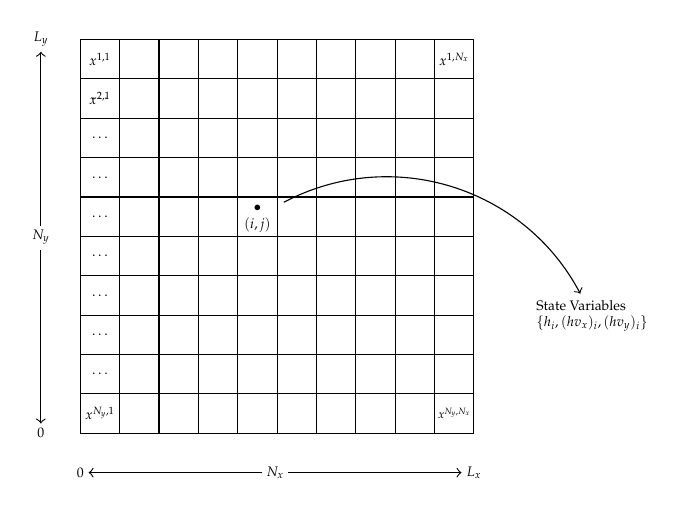
\begin{tikzpicture}[scale=0.5, every node/.style={transform shape}]
\foreach \x in {0,1,2,...,10}
\draw (\x,0) -- (\x,10);
\foreach \x in {0,1,2,...,10}
\draw (0,\x) -- (10,\x);
\node at (0.5,9.5){$x^{1,1}$};
\node at (0.5,8.5){$x^{2,1}$};
\foreach \x in {1,2,...,8}
\node at (0.5,\x+0.5){$\ldots$};
\node at (0.5,0.5){$x^{N_y,1}$};
\node at (9.5,9.5){$x^{1,N_x}$};
\node at (9.5,0.5)[scale=0.86]{$x^{N_y,N_x}$};
\node (A) at (0,-1){0};
\node (B) at (10,-1){$L_x$};
\node (C) at (-1,0){0};
\node (D) at (-1,10){$L_y$};
\draw[<->](A) -- (B)node[midway,fill=white]{$N_x$};
\draw[<->](C) -- (D)node[midway,fill=white]{$N_y$};
\node (E) at (4.5,5.5){\begin{tabular}{c}
$\bullet$ \\ 
$(i,j)$
\end{tabular}};
\node (F) at (13,3){\begin{tabular}{l} 
State Variables \\
$ \lbrace h_i,(hv_x)_i,(hv_y)_i \rbrace $
\end{tabular}};
\draw[->](E) to [bend left=45](F);
\end{tikzpicture}
\caption{$\textbf{X}$: Grid representation of DEM}
\label{grid_dem}
\end{center}
\end{figure}

\subsection{Uncertainty Modeling of the DEM}
\label{dem:uncertainty_model}
Uncertainty model of the DEM has to be accurate to enable an accurate estimation in the variation of the PHM. Modeling the spatial correlation in DEM requires modeling the difference or error maps~\cite{ehlschlaeger1994uncertainty, stefanescu2012digital}. Due to the continuous nature of the actual terrain profile, it is imperative to model the terrain profile as a random field.

In the problem considered in this work, the terrain profile $D$ is modeled as a \textit{second order} Gaussian random field defined on $(\Omega_D, \mathcal{A}, P)$ such that:

\begin{equation}
|| D ||^2_{L_2 (\Omega_D, P)} = \int_{\Omega_D} D^2 dP(\tau) < \infty
\end{equation}

$D$ is characterized by a bounded symmetric and positive definite covariance function $C(\textbf{s})$ with $\textbf{s} \in \Omega_D$ given as,

\begin{equation}
C(\textbf{s}_1, \textbf{s}_2) = \exp{\left( \frac{\textbf{s}_1 - \textbf{s}_2}{a} \right)} \hspace{5mm} \textbf{s}_1, \textbf{s}_2 \in \Omega_D
\end{equation}

\subsection{Adjacency  Matrix and Clustering of Spatial Domain}
\label{dem_adjacency}
The solution of Equation~\ref{main_eq} (Section~\ref{governing}) is achieved by Finite Volume Method. The solution procedure involves discretizing the spatial domain into uniform or non-uniform grid and the equation is then solved on the cell-averages of each grid. For the purpose of computing the adjacency matrix, a uniform grid $\lbrace N_x, N_y \rbrace$ is used. This reduces the PDE in Equation~\ref{main_eq} to a system of Matrix Differential Equation (MDE) involving $3N_x N_y$ variables given as:

\begin{equation}
\label{mde}
\dot{\textbf{Y}} = f(\textbf{Y, D})
\end{equation}

\noindent where, $\textbf{Y} = [\textbf{H}, \textbf{HV}_x, \textbf{HV}_y]^T \in \mathbb{R}^{3N_x \times N_y}$ is the matrix involving the discretized state space. $\textbf{D} \in \mathbb{R}^{N_x \times N_y}$ is the discretized DEM profile, where each cell corresponds to the height of the terrain profile in the discretized domain. The function $f:\mathbb{R}^{3N_x \times N_y} \times \mathbb{R}^{N_x \times N_y} \rightarrow \mathbb{R}^{3N_x \times N_y}$ is implicitly dependent on $\textbf{D}$. The MDE representation in Equation~\ref{mde} is used to compute the adjacency matrix using the concept of statistical linearization~\cite{Mukherjee_2017,roberts2003random,banaszuk2011scalable}. To implement the linearization technique, the 2-D domain $\textbf{X}$ is vectorized to a 1-D domain of length $N = N_x N_y$ as depicted in  Figure~\ref{grid_vec}. Equation~\ref{mde} is vectorized using the \textit{vec} operator as:

\begin{equation}
\label{ode}
vec(\dot{\textbf{Y}}) = vec\left(f(\textbf{Y}, \textbf{D}) \right) = g(vec(\textbf{X}), vec(\textbf{D}))
\end{equation}

\noindent Equation~\ref{ode} is a system of ODE in $\mathbb{R}^{3N}$. To compute the adjacency, following relations are introduced. 
\begin{equation}
\begin{array}{c}
\textbf{Y}_1 = \textbf{H} \hspace{5mm} \textbf{X}_2 = \textbf{HV}_x \hspace{5mm} \textbf{Y}_3 = \textbf{HV}_y \\
\textbf{Y} = [\textbf{Y}_1, \textbf{Y}_2, \textbf{Y}_3] \hspace{5mm} g(\textbf{Y},\textbf{D}) = [g_1(\textbf{Y}_1,\textbf{D}), g(\textbf{Y}_2,\textbf{D}), g(\textbf{X}_3,\textbf{D})]^T
\end{array}
\end{equation}

\begin{figure}
\begin{center}
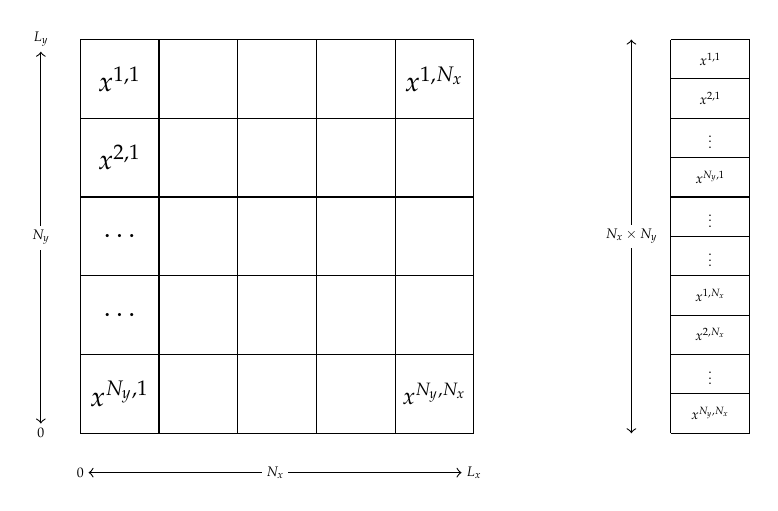
\begin{tikzpicture}[scale=0.5, every node/.style={transform shape}]
\foreach \x in {0,2,4,...,10}
\draw (\x,0) -- (\x,10);
\foreach \x in {0,2,4,...,10}
\draw (0,\x) -- (10,\x);
\node at (1,9)[scale=2]{$x^{1,1}$};
\node at (1,7)[scale=2]{$x^{2,1}$};
\node at (1,5)[scale=2]{$\ldots$};
\node at (1,3)[scale=2]{$\ldots$};
\node at (1,1)[scale=2]{$x^{N_y,1}$};
\node at (9,9)[scale=2]{$x^{1,N_x}$};
\node at (9,1)[scale=1.7]{$x^{N_y,N_x}$};
\node (A) at (0,-1){0};
\node (B) at (10,-1){$L_x$};
\node (C) at (-1,0){0};
\node (D) at (-1,10){$L_y$};
\draw[<->](A) -- (B)node[midway,fill=white]{$N_x$};
\draw[<->](C) -- (D)node[midway,fill=white]{$N_y$};
\foreach \x in {0,1,2,...,10}
\draw (15,\x) -- (17,\x);
\foreach \x in {15,17}
\draw (\x,0) -- (\x,10);
\node at (16,9.5){$x^{1,1}$};
\node at (16,8.5){$x^{2,1}$};
\node at (16,7.5){$\vdots$};
\node at (16,6.5){$x^{N_y,1}$};
\node at (16,5.5){$\vdots$};
\node at (16,4.5){$\vdots$};
\node at (16,3.5){$x^{1,N_x}$};
\node at (16,2.5){$x^{2,N_x}$};
\node at (16,1.5){$\vdots$};
\node at (16,0.5){$x^{N_y,N_x}$};
\draw[<->](14,0) -- (14,10)node[midway,fill=white]{$N_x \times N_y$};
\end{tikzpicture}
\caption{Grid to Vectorization of $\textbf{X}$}
\label{grid_vec}
\end{center}
\end{figure}

\noindent The definition of $g_1(\cdot), g_2(\cdot)$ and $g_3(\cdot)$ follows from the definition of $\textbf{F}, \textbf{G}$ and $\textbf{S}$ in Equation~\ref{defs}. To compute the adjacency, the approximate linear system matrix incorporating the information from $\textbf{X}_1, \textbf{X}_2$ and $\textbf{X}_3$ is given as,

\begin{equation}
\textbf{A}_{sl} = \sum_i^3 \int_{\Omega_{\textbf{D}}} \bigg| \frac{\partial g_i(vec(\textbf{Y}_i),vec(\textbf{D}_w))}{\partial vec(\textbf{Y}_i)} \bigg|_{vec(\textbf{X}_i) = vec(\textbf{X}_i)_0} dP_{\textbf{D}}(\textbf{D}_w) 
\end{equation}

Normalizing and symmetrizing the linear system $A$ results in the adjacency matrix $W$:

\begin{equation}
\label{adj_mat}
\textbf{W} = 0.5\textbf{R}^{-1}(\textbf{A}_{sl} + \textbf{R}\textbf{A}_{sl}^T \textbf{R}^{-1})
\end{equation}

\noindent where, $\textbf{R}$ is the degree matrix for $\textbf{A}_{sl}$. The clustering is performed by solving the following optimization problem~\cite{xie2013overlapping}

\begin{equation}
\label{louvain}
\begin{array}{rl}
\displaystyle \min_{\textbf{Z}} & Q_{ov}  = \frac{1}{2m}\sum_i \sum_{i,j \in c} \left[ A_{i,j} - \frac{k_i k_j}{2m} \right] z_{ic} z_{jc} \\
\displaystyle \text{subject to } & 0 \leq a_{ic} \leq 1 \hspace{5mm} \forall i \in V, \forall c \in C \\
& \displaystyle \sum_c^{|C|} a_{ic} = 1
\end{array}
\end{equation}

\noindent where $C = \lbrace c_1, c_2, \ldots, c_{|C|} \rbrace$ is the set of clusters and $\textbf{Z} = [a_{ij}]_{N \times |C|}$ determines the association of each state $i$ in cluster $j$. $Q_{ov}$ is an overlapping extension of the louvain-modularity function~\cite{blondel2008fast}. Each row of $\textbf{Z}$ corresponds to a particular region in the spatial domain of $\textbf{D}$. Once the $\textbf{Z}$ matrix is estimated, it is used with a given sampling scheme to generate the random samples for the DEM. 


\subsection{Random Sampling and Propagation}

The random sampling follows from the definition of Strongly Coupled Subsystems (SCSs) of a coupled dynamical system. In a system defined by an ode $\dot{\textbf{y}} = g(\textbf{y})$, $\textbf{y} \in \mathbb{R}^n$, $g:\mathbb{R}^n \rightarrow \mathbb{R}^n$, SCSs are defined as element of an overlapping partition of $\textbf{y}$ characterized by an association matrix $\textbf{Z}_{\textbf{x}} = \begin{bmatrix}
\textbf{z}_1 & \ldots & \textbf{z}_m
\end{bmatrix}$ as,
\begin{equation}
\label{hadprod}
\textbf{y} = \bigcup_j^m \textbf{x}_j|j \hspace{5mm} \textbf{y} = \sum_j^m \textbf{z}_j \odot \textbf{y}_j \hspace{5mm} \textbf{y}_j = \begin{bmatrix} \textbf{y}_j|j^T & \textbf{y}_j|j'^T \end{bmatrix}^T \in \mathbb{R}^n
\end{equation}

\noindent such that the SCS $\textbf{y}_j|j \in \mathbb{R}^{n_j}$ can be propagated in parallel and the manifold is defined by the following set of equations

\begin{equation}
\dot{\textbf{y}}_j|j = g_j (\textbf{y}_j|j) \hspace{5mm} g_j:\mathbb{R}^{n_j} \rightarrow \mathbb{R}^{n_j} \hspace{5mm} j = 1 \text{ to } m \hspace{5mm} \sum_j n_j \geq n
\end{equation}

\noindent At any time instance $t \in [0,\infty)$, the mean and covariance of $\textbf{y}$ is preserved under the Hadamard product relation (Following Equation~\ref{hadprod}) as:

\begin{equation}
\label{had_prod}
\begin{array}{l}
E[\textbf{y}] = \sum_j^m \textbf{z}_j \odot E[\textbf{y}_j|j] \\ 
\textbf{cov}(\textbf{y}) = \sum_j^m (\textbf{z}_j\textbf{z}_j^T) \odot \textbf{cov}(\textbf{y}_j|j)
\end{array}
\end{equation}

$\textbf{Z}_{\textbf{x}}$ is estimated from $g$ and the initial distribution of $\textbf{x}$~\cite{Mukherjee_2017overlap}. An SCS $\textbf{x}_j|j$ is identified from $\textbf{Z}_{\textbf{x}}$ using a threshold value $\epsilon$ as:

\begin{equation}
\label{scs_def}
\textbf{y}_j|j = \lbrace x_i| z_{ij} > \epsilon \rbrace
\end{equation}
In this work, we extend this idea of SCS to sample the DEM based on the cluster structure $\textbf{Z}$ identified in Section~\ref{dem_adjacency}. The nodes in weighted graph defined in Equation~\ref{adj_mat} refers to the cells in the spatially discretized domain of $\textbf{D}$. Thus, an SCS identified (Equation~\ref{scs_def}) will be a collection of cells in the discretized domain corresponding to a geographic region in the $\Omega_{\textbf{D}}$. The domain of DEM $\Omega_D$ and hence $vec(\textbf{D})$ is thus partitioned into $m$ number of SCSs $\Omega_{\textbf{D}_i}$ and $vec(\textbf{D}_i)$ of length $N_j$ such that:

\begin{equation}
\Omega_{\textbf{D}} = \bigcup_j^m \Omega_{\textbf{D}_j} \hspace{5mm} \sum_j N_j \geq N
\end{equation}

This partition can be used to generate realizations of $\textbf{D}$. Instead of sampling the whole DEM, one can sample a single zone $\Omega_{\textbf{D}_i}$, keeping the rest of the DEM at its nominal value. 


\subsection{Sampling of a Zone}

The sampling is done on a subdomain $\Omega_{D_j}$ at a time. The covariance function $C(x,y)$ defined in Section~\ref{dem:uncertainty_model} admits a spectral decomposition as~\cite{ghanem2003stochastic}:

\begin{equation}
\label{cov_int}
C(\textbf{s}_1,\textbf{s}_2) = \sum_{l=0}^\infty \lambda_l f_l(\textbf{s}_1) f_l(\textbf{s}_2) \hspace{5mm} \textbf{s}_1,\textbf{s}_2 \in \Omega_{D_j}
\end{equation}

\noindent where, $\lambda_l$ and $f_l(\textbf{s})$ are solutions to the following integral equation

\begin{equation}
\int_{\Omega_{D_j}} C(\textbf{s}_1,\textbf{s}_2) f_l(\textbf{s}_1)d\textbf{s}_1 = \lambda_l f_l(\textbf{s}_2)
\end{equation}

The variable $D$ for the subdomain $\Omega_{D_j}$ can be written as,

\begin{equation}
\label{kl_full}
D(\textbf{s}) = \mu_D(\textbf{s}) + \sum_{l=0}^\infty \xi_l f_l(\textbf{s}) \hspace{5mm} \xi_l = \int_{\Omega_{D_j}} (D(\textbf{s}) - \mu_D(\textbf{s}) )f_l(\textbf{s})d\textbf{s}
\end{equation}

\noindent where, $\xi_l$ are zero mean uncorrelated random variables with variance as $\lambda_l$. In practice, the summation in Equation~\ref{kl_full} is truncated up to a certain order $M$~\cite{ghanem2003stochastic} as

\begin{equation}
\label{kl_trunc}
D(\textbf{s}) = \mu_D(\textbf{s}) + \sum_{l=0}^M \xi_l f_l(\textbf{s})
\end{equation}

 
Analytical solution to the equation~\ref{cov_int} exists only for certain covariance functions. Numerical methods~\cite{atkinson2009numerical,hansen1992numerical} for solving Equation~\ref{cov_int} involves the evaluating the function $C(\textbf{s})$ for the discretized space $\textbf{X}$ defined in Section~\ref{highres}. This leads to solving the following eigenvalue problem: 

\begin{equation}
\textbf{C}_j\textbf{W}_j \textbf{f}_l = \lambda_l \textbf{f}_l
\end{equation}

\noindent where, $\textbf{C}_j$ and $\textbf{W}_j$ are $N_j \times N_j$ matrices given as


\begin{equation}
\label{cov_mat}
\resizebox{0.9\textwidth}{!}{%
$\textbf{C}_j = \begin{bmatrix}
C(x_j^{1},x_j^{1}) & C(x_j^{1},x_j^{2}) & \ldots & C(x_j^{1},x_j^{N_j}) \\
 & C(x_j^{2},x_j^{2}) & \ldots & C(x_j^{2},x_j^{N_j}) \\
& \vdots & \ddots & \vdots \\
&  &  &   C(x_j^{N_j},x_j^{N_j})
\end{bmatrix}
\textbf{W} = \begin{bmatrix}
1/N_j & 0 & \ldots & 0 \\
& 1/N_j & \ldots & 0 \\
 & \vdots & \ddots & \vdots \\
 & 0 & & 1/N_j
\end{bmatrix}$}
\end{equation}

Once the $M$ eigenvalues $\lambda_l$ and eigenvectors $\textbf{f}_l$'s are computed, sampling of $D$ gets reduced to generating realizations for $M$-dimensional $\xi = \lbrace \xi_1,\xi_2,\ldots, \xi_M \rbrace$.

Although, the above method is easy to implement, it is computationally expensive for high resolution DEMs that encompasses the full domain $\Omega_{D}$. The SCS identification-based method enables to sample the sub-regions in parallel with fewer realizations maintaining the same accuracy. This SCS-based sampling procedure can be used to sample a realization for the whole domain $\Omega_j$ by sampling a single zone $\Omega_j$ at a time. Algorithm~\ref{sample_dem} describes the overall procedure of clustering, sampling, propagation, and estimation of moments for a given cluster structure.


\begin{algorithm}[H]
\caption{Clustering of DEM using SCS and Propagation}
\label{sample_dem}
\begin{algorithmic}
\Require $C_\textbf{D}(x,y)$, $\textbf{Z}$, $N_x$, $N_y$, $\Omega_{\textbf{D}_j}$'s $j = 1$ to $m$
\Ensure $E(\textbf{U})$, $\textbf{cov}(\textbf{U})$ at each time
\ForAll{t}
\ForAll{j}
\State Sample $D_j(\textbf{s}), \textbf{s} \in \Omega_j$ using Equation~\ref{kl_trunc}
\State Create $D$ sample by keeping rest of the zones at $\mu(D)$
\State Propagate Equation~\ref{main_eq} for Zone $j$
\State Compute $E(\textbf{U})$ and $\textbf{cov}(\textbf{U})$ for Zone $j$
\EndFor
\State Compute $E(\textbf{U})$ and $\textbf{cov}(\textbf{U})$ at time $t$ using Equation~\ref{had_prod}
\EndFor
\end{algorithmic}
\end{algorithm}

\section{Generation of Realizations via Sampling Scheme}
\label{dem:uncertainty}
At each time instance, one is interested in computing the statistical properties of the pile height $h$ in Equation~\ref{main_eq} by evaluating multidimensional integral (Equation~\ref{monte_int}) of the form

\begin{equation}
\label{dem_monte_int}
E[h^a] = \int_{\Omega_D}  h^a(D) p_{D}(D) dD \approx  \frac{1}{\mathcal{N}}\sum_i^\mathcal{N} h^a(\mathcal{D}_i)
\end{equation}

The above integral is solved using sampling or quadrature based techniques described in Chapter~\ref{chap:uq}. In this reported work, the Latin Hypercube Sampling method~\cite{iman2008latin} has been used for generating the sampling space to compute the integral Equation~\ref{dem_monte_int}.

\section{Volcanic Locations}
\label{volcanic_location}
To implement the methodology explained in Section~\ref{dem_adjacency}, two volcanic locations are chosen, whereby the simulation of debris or avalanche flow resulting from a volcanic eruption on a realistic topography is demonstrated. For each location, the cluster structure as per Section~\ref{dem_adjacency} is computed and the DEM realizations are generated by Algorithm~\ref{sample_dem}. To understand the dependency of the cluster structure on the resolution $\lbrace N_x, N_y \rbrace$, a comparison of the cluster structure with the resolution of discretization has been performed.
After fixing a cluster structure for a given resolution, it is used to sample realizations.
For each realization in a cluster, the flow equation in~\ref{main_eq} is propagated. The average pile height is computed at each time to construct the PHM.

\subsection{Colima}

The Volcan de Colima~\cite{luhr1981colima} erupted in 1991, creating an impact up to a distance of 4 km. This phenomenon has been studied and simulated several times~\cite{rupp2003colima,pitman2003computing,rupp2006colima}. Figure~\ref{fig:colima} shows the extent of the colima region and the elevation profile of the region of interest. The Colima DEM is a $4.5 \text{km} \times 4.5\text{km}$ control region of resolution $5 \text{m}$. In the current setup, a cylindrical pile deposition of approximately $10^6$ $\text{m}^3$ is considered. The angle of frictions are assumed to be $\phi_{bed} = 27^\circ$ and $\phi_{int} = 37^\circ$. 

\begin{figure}[H]
\begin{subfigure}{0.4\textwidth}
\centering
\includegraphics[width=\textwidth]{dem_figs/colima_4}
\caption{}
\label{colima_1}
\end{subfigure}
\centering
\begin{subfigure}{0.55\textwidth}
\includegraphics[width=0.9\textwidth]{dem_figs/colima_el}
\caption{}
\label{colima_2}
\end{subfigure}
\caption{Geographic region of Volcan de Colima, showing the (a) control region and initial pile deposit location and (b) the elevation profile of the control region.}
\label{fig:colima}
\end{figure}

The $5m$  DEM is downscaled to different resolutions to compute the adjacency.
Figure~\ref{fig:colima_adjacency} shows the plot of the matrix $W$ for each resolution $\lbrace N_x, N_y\rbrace$. The plots are highly sparse as the resolution increases. Figure~\ref{fig:colima_cluster} shows the clusters detected in the control region. The cluster structure asymptotically converges with the resolution of discretization, and hence the original $5$ m DEM is not required in practice for the cluster generation. Since the cluster boundaries are fairly discernible with in $100$ m and $150$ m DEMs, the higher resolution cluster structure can be well interpolated from these maps. Also, the cluster structure corresponds to different height levels. This shows that the spatial correlation produces better effect on the cluster map. This cluster structure is now used to generate the realizations for each of the zone in parallel. 

\begin{figure}[H]
\begin{subfigure}{0.48\textwidth}
\centering
\includegraphics[width=\textwidth]{dem_figs/colima_adjacency_300}
\caption{Adjacency with 300 m resolution}
\label{colima_adjacency_300}
\end{subfigure}
\centering
\begin{subfigure}{0.48\textwidth}
\includegraphics[width=\textwidth]{dem_figs/colima_adjacency_225}
\caption{Adjacency with 225 m resolution}
\label{colima_adjacency_225}
\end{subfigure} \\
\begin{subfigure}{0.48\textwidth}
\centering
\includegraphics[width=\textwidth]{dem_figs/colima_adjacency_150}
\caption{Adjacency with 150 m resolution}
\label{colima_adjacency_150}
\end{subfigure}
\centering
\begin{subfigure}{0.48\textwidth}
\includegraphics[width=\textwidth]{dem_figs/colima_adjacency_100}
\caption{Adjacency with 100 m resolution}
\label{colima_adjacency_100}
\end{subfigure} 
\caption{Adjacency Matrix for Volcan de Colima using different resolutions of discretization.}
\label{fig:colima_adjacency}
\end{figure}

\begin{figure}[H]
\begin{subfigure}{0.48\textwidth}
\centering
\includegraphics[width=\textwidth]{dem_figs/colima_cluster_300}
\caption{Cluster structure with 300 m resolution}
\label{colima_cluster_300}
\end{subfigure}
\centering
\begin{subfigure}{0.48\textwidth}
\includegraphics[width=\textwidth]{dem_figs/colima_cluster_225}
\caption{Cluster structure with 225 m resolution}
\label{colima_cluster_225}
\end{subfigure} \\
\begin{subfigure}{0.48\textwidth}
\centering
\includegraphics[width=\textwidth]{dem_figs/colima_cluster_150}
\caption{Cluster structure with 150 m resolution}
\label{colima_cluster_150}
\end{subfigure}
\centering
\begin{subfigure}{0.48\textwidth}
\includegraphics[width=\textwidth]{dem_figs/colima_cluster_100}
\caption{Cluster structure with 100 m resolution}
\label{colima_cluster_100}
\end{subfigure} 
\caption{Cluster structure for Volcan de Colima using different resolutions of discretization.}
\label{fig:colima_cluster}
\end{figure}

Figure~\ref{fig:colima_simulate} shows the mean pile height $E(\textbf{U})$ at different time instance of the simulation. The hazard flow (in blue) is represented on a gray-scale image of the volcanic location to show its spread. The mean height is calculated for each zone in parallel and then the overall height is computed using the Hadamard product formula of Equation~\ref{had_prod}.

\begin{figure}[H]
\centering
\begin{subfigure}{0.46\textwidth}
\centering
\includegraphics[width=\textwidth]{dem_figs/newres_1}
\caption{at Time = 1s}
\end{subfigure}
\begin{subfigure}{0.46\textwidth}
\centering
\includegraphics[width=\textwidth]{dem_figs/newres_13}
\caption{at Time = 13s} 
\end{subfigure} \\
\begin{subfigure}{0.46\textwidth}
\centering
\includegraphics[width=\textwidth]{dem_figs/newres_25}
\caption{at Time = 25s}
\end{subfigure}
\begin{subfigure}{0.46\textwidth}
\centering
\includegraphics[width=\textwidth]{dem_figs/newres_37}
\caption{at Time = 37s}
\end{subfigure}
\caption{Mean Pile height at different time instance}
\label{fig:colima_simulate}
\end{figure}

To establish the accuracy of the SCS-based UQ, error plots have been plotted. A full model sampling space has been generated using Latin-Hypercube sampling. Spatial error in terms of the average pile height between the full model and the SCS-based model has been computed using the metric given as:

\begin{equation}
\epsilon_{\textbf{U}} = \frac{|E(\textbf{U})_c - E(\textbf{U})_f|}{\max_{\Omega_{D}} (E(\textbf{U})_f)}
\end{equation}

\noindent where, $E(\textbf{U})_c$ is computed from the SCS-based model and $E(\textbf{U})_f$ is computed from the full sampling scheme. Figure~\ref{fig:colima_error} shows the plot of $\epsilon_{\textbf{U}}$ for the volcanic region at different time instance. The color-bar at the side of each plots show the range of the value. The normalized error value ranges from 0.01 to 0.14 establishing the high efficiency of the SCS-based method in maintaining the accuracy of PHM estimation for a parallel sampling scheme. 


\begin{figure}[H]
\centering
\begin{subfigure}{0.46\textwidth}
\centering
\includegraphics[width=\textwidth]{dem_figs/fig1}
\caption{at Time = 1s}
\end{subfigure}
\begin{subfigure}{0.46\textwidth}
\centering
\includegraphics[width=\textwidth]{dem_figs/fig13}
\caption{at Time = 13s} 
\end{subfigure} \\
\begin{subfigure}{0.46\textwidth}
\centering
\includegraphics[width=\textwidth]{dem_figs/fig25}
\caption{at Time = 25s}
\end{subfigure}
\begin{subfigure}{0.46\textwidth}
\centering
\includegraphics[width=\textwidth]{dem_figs/fig37}
\caption{at Time = 37s}
\end{subfigure}
\caption{Mean Pile height at different time instance}
\label{fig:colima_error}
\end{figure}

\section{Summary}

This chapter outlines the methodology in identifying sub-regions that contribute independently in parallel to the overall hazard map resulting from the geophysical mass flow simulation. The independent regions bears regional overlap that can be quantified using the suitable clustering method. Titan2D provides a robust platform to integrate with the proposed sampling scheme for generation of the PHMs. The outlined framework is able to achieve the target of generating sampling space in parallel as compared to any other sampling scheme for the same level accuracy. Computation of moments from the results of the CFD simulations can also be performed faster compared to traditional methods. It is shown that the applicability of SCS detection is universal in terms of sampling scheme. In other words SCS-based UQ approach can be integrated with any given sampling scheme. Some possible avenues for future works is discussed next.

In contrast to polynomial or exponential growth in standard cubature-based methods~\cite{stroud1971approximate}, the SCS-based method can produce a linear growth in number of collocation points with increase in the size of the problem. Thus, producing PHMs by integrating SCS-based UQ with cubature-based methods can be a scope of future work.

Even with the advantage of faster computation with the sampling scheme, formulation of the adjacency matrix can still be a non-trivial due to the size of the DEM. The current clustering paradigm takes advantage of asymptotic convergence of the cluster structure with increase in the resolution of the discretization. The adjacency formulation relies on vectorization and application of standard clustering techniques. The framework can be extended by taking the fourth order tensor adjacency followed by application of tensor-based overlapping community detection methods~\cite{benson2015tensor,shashua2005non,huang2013fast}.  

The SCS-based method has been useful for not only faster UQ but also in breaking the overall stochastic problem into subproblems. To incorporate the idea of subproblem decomposition into the PHM computation problem, one has to carefully define the boundary conditions in the identified subproblem, such that solving them in parallel bears a meaningful physical interpretation with respect to the full model. 
\chapter{Conclusion and Future Works}
\label{chap:conclusion}

In this chapter, insights gathered from previous chapters are summarized. Additionally, avenues for future research directions are also outlined. Chapter~\ref{chap:wcs} discusses the details of \textit{linearization and clustering} methods that has been used throughout the dissertation. Answers pertaining to several questions about the usage of \textit{linearization and clustering} methodology are outlined next:

\textit{How do the differences in the methods of Linearization effect the overall performance of propagation of uncertainty?} The results of clustering differ with different methods of linearization. The concept of average linearization is based on the assumption that the methodology is able to capture sufficient information for the clustering algorithm to be implemented. The concept of average Eigenvalues differ from the concept of average Jacobian in terms of periodicity of the system. If the system exhibits a limit cycle oscillation, then the ideal time window for averaging out the Eigenvalues should be the time period of the oscillation. This time window differs from problem to problem. Averaging out the Jacobian may not require such condition. However, one should notice that, while using linear coupling function, the Jacobian does not take into consideration the change in the state variables due to coupling. Hence, the detection of cluster will depend only on the value of the constant coupling strength and not on the time window. The Statistical Linearization is however a Jacobian free method and independent of the time window. As discussed earlier, it is the only method which is able to capture the effect of changing covariance, which may affect the result. Performance of both type of methods do not differ much, which establishes the fact that the Statistical Linearization is able to capture the same information of a nonlinear system as the Jacobian-based techniques. The method is also easier to implement, as it does not rely on the nominal trajectory as well. 

\textit{Which one of the seven methods is suitable?} Our work has proposed seven techniques combining two methods of graph clustering and four methods of linearization. From the ANOVA Table~\ref{anova}, it is evident that the contribution of the techniques towards the variability of the results is not high. Thus, the choice of the method entirely depends on two factors i) computational expense and ii) Reliability of the methods.

\textit{How are the performance and the reliability of the seven methods:} The linearization and clustering method together work excellent for weakly coupled oscillators. The error values for all the test cases with $e = 0$ are negligible. As pointed out earlier, the clustering technique accurately identifies the weakly coupled oscillators at each of the time instance. The linearization step involves the Jacobian computation, that captures the block-diagonal structure. Due to numerical values it may happen that an individual oscillator of two or three dimension can erroneously show more than one cluster. Averaging out the linearized system retains the appropriate block-diagonal structure. The clustering technique has to be flawless in identifying the blocks. However, the accuracy of Method II and III in capturing the block-diagonal structure immensely depend on the coupling strength and the accuracy of Algorithm~\ref{Eigenvect2}. Once that is done perfectly, the clustering algorithm works well in identifying the block. The accuracy of the methods in identifying decoupled oscillators is very high and results in very small error values. The small error values arise due to numerical computation. With increase in the value of $\epsilon$, the effectiveness of the Statistical Linearization increases. 

For a fixed initial condition, the Jacobian-based linearization techniques involve a deterministic scheme to form the graph adjacency matrix. Thus, the randomness in the technique is induced from the randomness of the clustering technique. The last step of Spectral Clustering, which involves k-means clustering, and NMF, both require generating an initial random seed. Also, as it has been pointed out, if the clustering technique fails, even at a single time instance, then cumulative error becomes huge. 

\textit{What is the computational expense of each of the methods?} Out of the seven proposed techniques, four of them are based on Eigenvalue computation. Method II and III of linearization involve Eigenvalue computation at each step. With the increase in dimensionality, the Eigenvalue computation becomes very expensive. Also, the convergence of numerical methods of Eigenvalue computation for a high dimensional sparse matrix is itself a challenging problem. On the other hand, the Bayesian NMF requires an iterative procedure for finding the best possible solution, which requires much less computational time than the Eigenvalue computation. Linearization method I-III also requires the estimation of the nominal trajectory. The one-point Statistical Linearization proves to be computationally inexpensive compared to the other methods. 

\textit{What are the effects of different factors?}  The ANOVA (Table~\ref{anova}) shows the effect of factors on the performance of the algorithms. The p-values against the effect of $N$, $e$, and methods of Linearization and Clustering show the robustness of the method. Despite showing apparent differences in the numerical values, the contributions of each of these factors to the variability of the performance is shown to be statistically insignificant. Thus, we fail to reject the null Hypothesis, that the error generated in the current methodology is independent of the dimensionality, coupling strength, and the method of linearization and clustering. The p-values against the other main effects seem to quite high. Thus, we reject the null hypothesis for `Type of Problem'. 

\textit{What if the coupling functions are different or the coupling strength is high?} The current study is restricted to diffusive coupling. In the linear system, due to the cyclic diffusive coupling function, one is able to derive suitable properties and get a good understanding of the system. The algebra of the system helps us to infer the pattern of the propagation of the cluster. With that idea, diffusive coupling has been used in nonlinear systems also. The coupling strengths have been reduced so as to obtain proper cluster structure. It has also been noted that with the increase in coupling strength, the value of error increases. The simple Jacobian can be replaced by the State Transition Matrix (STM), and it can be hypothesized, that the effect of coupling can be better captured. STM gives an advanced idea of the future cluster structure with respect to the previous state. Hence, the predictive model can be made better. However, with STM, the computational expense for the Statistical Linearization-based method becomes exceptionally huge. 



Chapter~\ref{chap:scs} relaxes the binary association theory the WCS framework to a fuzzy association framework to detect Strongly Connected Subsystems (SCSs). In this context following research questions have been addressed in the dissertation:

%\textit{How accurate is the assumption of the summation of element-to-element product?}
The accuracy of the element-to-element or Hadamard product lies in the assumption of linear relationship of the estimated association values with the adjacency matrix. Thus, the method accurately estimates the deterministic and as well as uncertain flow in the Shallow Water model because of the linearity in the original model of Equation~\ref{swe_discrete}. For a nonlinear model, the association values are to be periodically updated with availability of measurement, or after a certain period of time. 

In the work reported in Chapter~\ref{chap:building}, a reduced-order thermal model has been developed, using the lumped capacitance RC network model to calculate the load the HVAC system. Using the RC network model in conjunction with the Weakly Connected Subsystems optimal estimation method, we are able to provide a condensed framework for estimating internal loads, solar heat gains, and HVAC supply air temperatures in BEM.  Furthermore, one can use the developed method to calculate the uncertainty of the results for a comprehensive representation of the building systems.
One significant advantage of the presented methodology in Chapter~\ref{chap:building} is the ability to reduce the computation expense of large-scale dynamical systems while maintaining accuracy and providing uncertainty information at each step.  

It is shown that the overlapping clustering method detailed in Chapter~\ref{chap:scs} is proved to be effective for not only state space decomposition but also for clustering a random field. Each cluster of random field is shown to require less number of eigenvalues for approximate KL expansion when compared the whole field. Thus, the clustering not only aids in reduced sample points for the state space but also for the random field.

%As mentioned in Chapter~\ref{chap:wcs}, the search for an ideal clustering technique is never ending. It is to be noted that in the later two chapters, the preferred method of clustering got shifted to Louvain Modularity Optimization than SC or NMF. 

The two application problems used in this dissertation are in two somewhat distinct engineering domain. The applicabilities of the developed methods show the usage of the \textit{linearization and clustering} methods in UQ of most of the physics-based model. As mentioned earlier, the SCS-based UQ method did not show a significant improvement in the performance for the coupled oscillator problem. This result motivated us to use the WCS-based UQ method for the BEM problem. Results are promising and can be interpreted very easily. The WCS-based UQ was earlier applied to PDE problems without much success. Due to the failure of WCS-based UQ approaches to meaningfully solve PDE problems, the results of applied WCS based UQ methods on PDE problems were not reported in this dissertation. The development of the SCS-based UQ methods allows us to tackle the PDE problems. The linear Shallow Water Equation showed satisfactory performance with the use of SCS-based UQ method. The DEM problem is also shown to work very effectively within the SCS-based UQ framework. It is to be noted that the applicability of the SCS-based UQ slightly differ in the 1D linear Shallow Water Equation than the 2D Geophysical Mass Flow equation. 

\section{Future Works}

Analyzing the overall work, some of the future works pertaining to the dissertation are as follows:

\textit{What are the physical interpretation of the cluster structure?} The discussed methods are very instrumental in detecting decoupled oscillators when the coupling strength is 0. However, the current methodology cannot guarantee absolutely zero error for highly coupled systems. Also, the current theoretical limitation compels us to resort to perform repetitive numerical simulations and statistical analysis. Ascertaining whether the identified WCSs according to the current framework has any physical interpretation in terms of the dynamics of the system is a scope of future work. 

\textit{Are the methods of linearization exclusive?} The four methods of linearization are instantaneous operators averaged over a given time window. As pointed out earlier, replacing the Jacobian with the State Transition Matrix can give us a better insight into the cluster structure, and is a scope of future work.  

\textit{How does the Hadamard product ensure the state-space decomposition for a nonlinear system?} Currently the method relies on an intuitive assumption and proof by numerical methods only. The 1D Shallow water equation shows good result for both deterministic and probabilistic cases. A rigorous mathematical proof showing the convergence of the Hadamard product to the actual result for a linear system and its extension to nonlinear system can be a scope for future work. The nonlinearity in the geophysical mass flow problem has restricted us from performing the state-space decomposition. A decomposition could unnecessarily bring complication in tackling the boundary conditions of the subproblems, if not properly defined. 

A repository of the codes summarizing the framework presented in this dissertation is currently in preparation. This repository is to include Statistical Linearization as the preferred method of linearization. The current choice of clustering method is Louvain Modularity Optimization. The repository is also designed to include different sampling and quadrature/cubature-based UQ methods. A Message Parsing Interface (MPI) support is also being designed for this research. Please check the following link for regular updates:
\begin{center}
{\tt \url{https://github.com/arpanisi/UQ_Dynamics}}.
\end{center}





\bibliographystyle{unsrt}
\addcontentsline{toc}{chapter}{Bibliography}
\bibliography{root,root_2,AllRefs,jbs,dem}
\end{document}
